% --- ADVANCED CONTROL TECHNIQUES ---
% ------------------------------------------------------
% Corso di Laurea Magistrale in: Ingegneria Informatica - Università Del Salento
% Titolo: Advanced Control Techniques
% Autore: Dott. Marco Chiarelli
% Relatore: Prof. Giuseppe Notarstefano
% Data: 31/05/2016
% Anno Accademico 2015/2016
% Consultazione Consentita

%INIZIO PREAMBOLO

\documentclass[11 pt,a4paper,twoside,openany]{book}

% Preambolo codifica
\usepackage[utf8]{inputenc}

%Preambolo lingue
\usepackage[english,italian]{babel}


% Preambolo formattazione
\usepackage[margin=1in,includefoot]{geometry}
\usepackage{indentfirst} %indentazione}

% Preambolo stile pagina
\usepackage{fancyhdr}

%Preambolo matematica
\usepackage{xfrac}
\usepackage{amsmath}
\usepackage{amsthm} % dopo amsmath!

% Preambolo grafico
\usepackage{float}
\usepackage{graphicx}
\usepackage{eso-pic}
\usepackage{tikz}
\usepackage[pages=some]{background}
\usepackage{transparent}

% Preambolo contenuti LoremIpsum
\usepackage{lipsum}

%hyperlinks
\usepackage[hidelinks]{hyperref}
\usepackage{hyperref}

%Preambolo bibliografia

\usepackage[numbers,sort&compress]{natbib}

%Preambolo licensa
%\usepackage{creativecommons}
\usepackage{ccicons}


%Preambolo testo
\usepackage{setspace}
\usepackage{epigraph}
\usepackage{ragged2e}
\usepackage{amsthm}
\usepackage{amssymb}

% Preambolo schema a blocchi
\usepackage{verbatim}

% Preambolo matematica
\usepackage{amsmath}
\usepackage{amsthm}
\usepackage{amssymb}
\usepackage{centernot}
\usepackage{accents}

\usepackage{mathtools}
\DeclarePairedDelimiter{\abs}{\lvert}{\rvert}
\DeclarePairedDelimiter{\norma}{\lVert}{\rVert}

\DeclareMathOperator{\Ima}{Im}
\DeclareMathOperator{\rank}{rank}
\DeclareMathOperator*{\argmin}{arg\,min}

\newtheorem{defn}{Definition}
\newtheorem{thrm}{Theorem}
\newtheorem{prop}{Proposition}
\newtheorem{lemma}{Lemma}
\newtheorem{corl}{Corollary}


\newcommand\inv[1]{#1\raisebox{1.15ex}{$\scriptscriptstyle-\!1$}}
\newcommand{\tendsto}[1]{\xrightarrow{\smash{\raisebox{0.10ex}{$\scriptstyle#1$}}}}
  

\newcommand{\numberset}{\mathbb}
\newcommand{\N}{\numberset{N}}
\newcommand{\Z}{\numberset{Z}}
\newcommand{\R}{\numberset{R}}
\newcommand{\C}{\numberset{C}}

\newcommand{\cball}{\bar{\mathbb{B}}}
\newcommand{\oball}{\mathring{\mathbb{B}}}

\newcommand*{\diff}{\mathop{}\!\mathrm{d}} %dichiarazione differenziale
\newcommand*{\im}{\mathop{}\!\mathrm{i}} %dichiarazione unit immaginaria
\newcommand*{\e}{\mathop{}\!\mathrm{e}} %dichiarazione unit nepero
\newcommand*{\imm}{\mathop{}\!\mathrm{Imm}} %immagine
\newcommand*{\id}{\mathop{}\!\mathrm{id}}
\newcommand*{\Span}{\mathop{}\!\mathrm{span}} %span
\newcommand{\sign}{\text{sign}}

\newcommand{\lapl}{\mathcal{L}}

\newcommand{\ctsys}{
\[
\left\{
\begin{aligned}
\dot{x}(t) &= f(x(t), u(t), t); \\
y(t) &= h(x(t), u(t), t);
\end{aligned} 
\right.
\\
\quad with\ x(t_0) = x_0;
\]
}

\newcommand{\dtsys}{
\[
\left\{
\begin{aligned}
x(t+1) &= f(x(t), u(t), t); \\
y(t) &= h(x(t), u(t), t);
\end{aligned} 
\right.
\\
\quad with\ x(t_0) = x_0;
\]
}

\newcommand{\lctsys}{
\[
\left\{
\begin{aligned}
\dot{x}(t) &= A(t)x(t) + B(t)u(t); \\
y(t) &= C(t)x(t) + D(t)u(t)
\end{aligned} 
\right.
\\
\quad with\ x(t_0) = x_0;
\]
}

\newcommand{\ldtsys}{
\[
\left\{
\begin{aligned}
x(t+1) &= A(t)x(t) + B(t)u(t); \\
y(t) &= C(t)x(t) + D(t)u(t)
\end{aligned} 
\right.
\\
\quad with\ x(t_0) = x_0;
\]
}

\newcommand*{\QEDA}{\hfill\ensuremath{\blacksquare}}
\newcommand*{\QEDB}{\hfill\ensuremath{\square}}

\newcommand{\cardinality}[1]{\left\vert{#1}\right\vert}

% Preambolo Inclusione Capitoli
\includeonly{chapters/intro,%
			 chapters/systheory,%
			 chapters/sysstab,%
			 chapters/distsys,%
			 chapters/algoptzs,%
			 chapters/training}

% Preambolo caption, subfig, etc...
\usepackage{caption}
\usepackage{subfig}

%FINE PREAMBOLO


%FINE PREAMBOLO

\selectlanguage{english}
\selectlanguage{italian}

%%%%%%%%%%%%%%%%%%%%%%%%%%%%%%%%%%%%%%%%%%%%%%%%%%%


\begin{document}



\pagestyle{fancy}
\fancyhead{}
\fancyfoot{}
\fancyfoot[R]{\thepage}
\renewcommand{\headrulewidth}{0pt}
\renewcommand{\footrulewidth}{0.1pt}

\newpage	
\begin{titlepage}
\begin{center}
	
\begin{figure}
	\centering
	
\includegraphics[height=6cm]{unigold.jpg}
\end{figure}		

\begin{center}
\begin{LARGE}
	\textsc{UNIVERSIT\`A DEL SALENTO}\\
	[0.2cm]
	\textsc{Department of Innovation Engineering}
\end{LARGE}
\end{center}	
	
	\
	\line(1,0){270} \\
	[0.25cm]
	
	\textsc{Master's degree in Computer Engineering}\
	
	\textsl{}\\
	[1cm]
	\textsc{Advanced Control Techniques}\
	
	\bigskip 
	\huge{\bfseries Advanced Control Techniques}\

	
	\bigskip
	\textsl{}\\
	[2cm]
	


\begin{LARGE}
	
	Dott. Marco Chiarelli
	
\end{LARGE}

\vspace{5cm}
	
\line(1,0){150} \\
\begin{small}
	Academic Year 2015/2016 \\
\end{small}
\end{center}
\end{titlepage}


\pagenumbering{arabic}

\newpage
\null\vspace{\stretch{1}}\vspace{\stretch{2}}\null

\newpage
Quest'opera è stata rilasciata con licenza Creative Commons Attribuzione - Non commerciale - Condividi allo stesso modo 3.0 Unported. Per leggere una copia della licenza visita il sito web http://creativecommons.org/licenses/by-nc-sa/3.0/ o spedisci una lettera a Creative Commons, 171 Second Street, Suite 300, San Francisco, California, 94105, USA.\par \ccbyncsaeu
	\vfill
	Questi appunti sono stati scritti utilizzando \LaTeX\ tramite la distribuzione MiKTeX\ \url{http://miktex.org/}  
	
	Come editor è stato usato TeXMaker 4.4.1\ \url{http://www.xm1math.net/texmaker/}
	\vfill
Dei contenuti rielaborati in questa opera, salvo esplicitamente scritto il contrario, il prof. Giuseppe Notarstefano non se ne assume alcuna responsabilità.

\null\vspace{\stretch{1}}\vspace{\stretch{2}}\null

\thispagestyle{fancy}
\fancyhead{}
\fancyfoot{}
\fancyfoot[C]{\thepage}
\vspace{2cm}

\selectlanguage{english}

\noindent

\chapter*{\centering\begin{normalsize}Sommario\end{normalsize}}
\begin{quotation}
\noindent Le seguenti dispense vogliono essere un resoconto didattico del corso di Advanced Control Techniques, il quale docente è il prof. Giuseppe Notarstefano, presso il CdL in Ingegneria Informatica at Unisalento. Il programma copre tre macro-argomenti: la Stabilità dei Sistemi Non Lineari, i Sistemi Distribuiti ed Algoritmi di Ottimizzazione (distribuiti), più un piccolo capitolo circa delle Esercitazioni. Il seguente lavoro non ha la pretesa di sistematizzare in maniera esatta ciò che è stato fatto a lezione, sebbene l'impostazione di base cerca di seguire fedelmente ogni singola lezione che è stata erogata. Piuttosto cerca di raccogliere in maniera sintetica ma al contempo esaustiva gli aspetti chiave della Teoria del Controllo Avanzato, di fare ordine tra una quantità non indifferente di nozioni, e soprattutto di dare un sussidio alla preparazione di un eventuale esame didattico che richieda la conoscenza di queste nozioni e relativa applicazione per quanto concerne il lato pratico.
\end{quotation}
\clearpage

\selectlanguage{english}

\chapter*{\centering\begin{normalsize}Abstract\end{normalsize}}
\begin{quotation}
\noindent The following work want to be a report about the Advanced Control Techniques course, whose teacher is the prof. Giuseppe Notarstefano, at. Computer Engineering @ Unisalento. The program covers three macro-topics: Non-Linear Systems' Stability, Distributed Systems, and (Distributed) Optimization Algorithms plus a little chapter that treats some Exercises. It won't systematize the entire work done at lessons in an exact manner, despite the base setting tries to follow each lessons that has been delivered to us. It tries to gather the key aspects of the Advanced Control Theory, and to reorder some difficult notions. Moreover it tries to give an help for the preparation of an eventual didactic exam that requires the knowledge about these notions and the related practical applications/homework/exercises.
\end{quotation}
\clearpage

\selectlanguage{italian}

\tableofcontents


\frontmatter

\cleardoublepage\thispagestyle{empty}
\vspace*{\fill}
\begin{center}
\bfseries Ringraziamenti
\end{center}
\bigskip

Un grazie particolare va ai miei compagni\\
d'università, Dino Sbarro, Gabriele Accarino, Giampiero D'Autilia, Matteo Settembrini, Paolo Panarese ed Emanuele Costa Cesari.

\vspace*{\fill}
\pagebreak

%************************************************
% Chapter 0: INTRODUCTION
%************************************************
% !TEX encoding = UTF-8
% !TEX TS-program = pdflatex
% !TEX root = ../nt.tex
% !TEX spellcheck = it-IT

%************************************************
\chapter{Introduzione}
\label{cap:intro}
%************************************************\\

\begin{itemize}

\item{\textbf{Prerequisiti}}

Buona conoscenza di linguaggi \textit{Object-Oriented} (almeno uno), tecniche e strumenti. Elementi di computer networks e tecnologie di Rete, Web;

\item{\textbf{Abilità acquisite}}

Lo studente sarà in grado di progettare e capire i modelli dei dati, creare e gestire database e progettare ed implementare applicazioni data-centric.

\end{itemize}

Lo scopo è fornire le basi circa le principali teorie sui database, tecniche e strumenti per \textbf{usare} i database e \textbf{progettare/implementare} database \textbf{applications}.

\textbf{Argomenti}:

\begin{itemize}

\item Database, database relazionali, NoSQL e NewSQL;
\item Sistemi di gestione dei database (DBMS);
\item Modello Relazionale ed Algebra Relazionale;
\item SQL: definizioni dei dati e loro manipolazioni;
\item Basi della Computer-Human Interaction e progettazione delle interfacce;
\item Aspetti architetturali: Clients, Servers, Peers, Dispositivi, IoT, ...
\item Principi di Data-Analytics;
\item Analisi multidimensionale e data-warehouse;

\end{itemize}

\mainmatter

%************************************************
% Chapter 1: SYSTEMS' THEORY
%************************************************
% !TEX encoding = UTF-8
% !TEX TS-program = pdflatex
% !TEX root = ../act.tex
% !TEX spellcheck = it-IT

%************************************************
\chapter{Systems' Theory}
\label{cap:systheory}
%************************************************\\

\section{Systems' Classes}

We will identify a class of systems. The SETUP we will play with is the so-called State-Space FRAMEWORK. 

\begin{equation}
\left\{
\begin{aligned}
& CONTINUOS-TIME\ SYSTEMS \\
& DISCRETE-TIME\ SYSTEMS \\
\end{aligned} \\
\right.
\end{equation}

, where for the CONTINUOS-TIME SYSTEMS we have this settings:

\begin{equation}
\left\{
\begin{aligned}
ODE:\ &\dot{x}(t) &=\ f(x(t),u(t),t) \\
OUTPUT:\ &y(t) &=\ h(x(t),u(t),t) \\
\end{aligned}
\right.
\end{equation}

, with $\underline{t \in \R}$, typically with $(t \geq t_0)$ (in some situation we could have $t < 0$), $\ x(t) \in \R^n$ as the STATE OF THE SYSTEM, $u(t) \in \R^m$ as the INPUT OF THE SYSTEM, $y(t) \in \R^p$ as the OUTPUT OF THE SYSTEM, and let $x(t_0) = x_0$ be the initial condition at the initial time instant $t_0$.
Typically we have UNDER-ACTUATED systems, in the sense that $m \leq n$, as there are also OVER-ACTUATED systems: $m > n$. The input is something that can modify the behavior of the system. $u := DECISION\ VARIABLE$. $x(t)$ is instead something that will be used to describe the behavior of the system. Concerning output, e could have two types:

\begin{equation}
\left\{
\begin{aligned}
& MEASURED\ OUTPUTS \\
& PERFORMANCE\ OUTPUTS \\
\end{aligned} 
\right.
\end{equation}

\begin{itemize}

\item MEASURED OUTPUTS: When describing a system of state, it is possible that we may not observe some variables. For example, suppose a quadrotor system:

\begin{equation}
\left\{
\begin{aligned}
P_x,\ P_y,\ P_z,&\ \dot{P_x},\ \dot{P_y},\ \dot{P_z}\\
(\Phi,\ \theta,\ \psi),&\ (\omega_1\ \omega_2\ \omega_3)
\end{aligned} 
\right.
\end{equation}

Suppose the quadrotor is equipped with a giroscope. $(\underline{\omega_1,\ \omega_2,\ \omega_3})$ are available. It may have sense to measure $P_z$ (altitude), but some output cannot be measured without a sensor. Something obtained by a sensor is a  MEASURED OUTPUT;

\item PERFORMANCE OUTPUTS: Assign a desired behavior. We want, for example, the quadrotor to do a complete flip. There is a part of the state to which we want to ASSIGN A DESIRED BEHAVIOR. In this example, it may be the angular part of the state.

\end{itemize}

Concerning inputs, we can also classify them into two types:

\begin{itemize}

\item CONTROL INPUT, that will be able to change behavior of the system (ex. the state) if we have an actuator;
\item DISTURBANCE: we can't affect it and typically we cannot measure it. We have to take it into account when designing a control law.

\end{itemize}


Concerning the design of a control law... what is $\{f(\mathord{\cdot}),\ h(\mathord{\cdot})\}\ =\ ??$. Let's introduce some notions:

\subsubsection{Continuous Time Sytems}

\underline{ODE} stands for (Ordinary Differential Equation). Typically it is of the FIRST ORDER because we have only one derivative of the state vector. This is a general case, because we can always reconduct ourself in this case; Let: $\dot{x}(t) := \frac{d(x)}{dt}$. In the general case we have:

\begin{equation}
\left\{
\begin{aligned}
\dot{x}(t) &= f(x(t), u(t), t) : \R^n\times\R^m\times\R \mapsto \R^n\\
y(t) &= h(x(t), u(t), t) : \R^n\times\R^m\times\R \mapsto \R^p
\end{aligned} 
\right.
\\
\quad with\ x(t_0) = x_0
\end{equation}

Now the question is.. what kind of properties these functions we'll need? 
The more assumption we put to $f$, the easier will be the design of the control law of the actual system; in fact it should not be TOO MUCH SIMPLE, otherwise the design process will be difficult.

\subsubsection{Discrete Time Systems}

In this case, the time is an integer variable: $(t \in \Z) \geq t_0$ (typically we will play with $\N = \Z^+$) is some sort of time, but clearly there are some differences! 

\begin{equation}
\left\{
\begin{aligned}
x(t+1) &= f(x(t), u(t), t) : \R^n\times\R^m\times\R \mapsto \R^n; \\
y(t) &= h(x(t), u(t), t) : \R^n\times\R^m\times\R \mapsto \R^p;
\end{aligned} 
\right.
\\
\quad with\ x(t_0) = x_0
\end{equation}


\underline{FDE} stands for (Finite Difference Equation). Why it is important to point out this in discrete time system? 

\begin{itemize}
\item There could be dynamical systems like the CLOCK (ex. the CLOCK of our machine), which are intrinsically DISCRETE;
\item It is more convenient to discretize an ODE with a FDE, actually converting a continuos-time system into a discrete time one;
\item Algorithms are discrete-time systems (ex. Optimization Problems Solving). So we will actually work treating them a algorithm to study for example its CONVERGENCE.
\end{itemize}

This is the framework. Obviously it doesn't cover all type of actual systems. (Complex multi-agent systems, Hybrid systems). This is only a class of possible models.
An important property that our systems have is the so-called MARKOV PROPERTY: generally more clear for discrete time systems. The evolution of our systems from time $t_0$ is entirely defined by the initial state $\{x(t_0) = x_0,\ u : [t_0, \infty) \mapsto \R^m\}$, where $u$ is the EVOLUTION OF THE INPUT.
The history of the state doesn't play any role! Once assigned $x_0$ and $u : [t_0, \infty) \mapsto \R^m$, IT DOESN'T MATTER! The solution is clearly defined. Suppose we want to compute, for example:

\[
x(2) = f(x(1),u(1),1),\ x(1) = f(x(0),u(0),0),\ t_0 = 0,\ x(0) = x_0
\]

but $x(1)$ is KNOWN. By keeping going further we could map the entire state evolution. It is clear this for discrete time systems, but under some assumptions (the Cauchy theorem) this property holds also for continuos time systems.

Cauchy Theorem: (\underline{ODE} under some assumptions have unique solution).

\ctsys

Note that classifications given for continuos time systems hold also for DT systems.
This general system can be identified as:

TIME-VARYING, NON LINEAR, PROPER FORCED SYSTEM. This is the most general system we can play with. Suppose $f$ is a regular function. For example any NL function. we will identify a set of subclasses of system, for which we assume consequently something more.
Note that: $FORCED \iff (u(t) \neq 0)$ (that can affect the behavior of system).
If we restrict the possible functions, then clearly we'll have less systems that can be modeled with these.

\subsection{TIME-VARYING vs TIME-INVARIANT SYSTEMS}

What it actually means in terms of evolution of system? Suppose we have:

\[
	x(t_0) = x_0\ as\ CINIT,\ \bar{u} : [t_0, +\infty) \mapsto \R^m\ as\ INPUT
\]

Let's suppose $f$ is sufficiently regular. $\bar{x}: [t_0, \infty) \mapsto \R^n\ as\ STATE\ EVOLUTION,\ \dot{\bar{x}} = f(\bar{x}(t), \bar{u}(t), t),\ \bar{x}(t_0) = x_0$ is TRUE! IT IS SATISFIED as $\bar{x}$ is the solution of the ODE. Moreover we have the (UNIQUENESS OF THE SOLUTION of the ODE).
Vediamo ora cosa succede partendo da CINIT uguali e da INPUT uguali ma applicati in istanti diversi.
Let's suppose:

\[
	\bar{u}_1 : [t_0 + t_1, +\infty) \mapsto R^m
\]

such that $\forall t \geq t_0 + t_1$, the $\bar{u}_1(t) = \bar{u}(t-t_1)$. The system is time-invariant then the state evolution is:

\[
	\bar{x}(t-t_1), \forall t \geq t_0 + t_1
\]

So applying $\bar{u}(\mathord{\cdot})$, we get $\bar{x}(\mathord{\cdot})$. (TIME-INVARIANT): if we start from the same CINIT then my state evolution will be a translated version of the previous $\bar{x}(\mathord{\cdot})$. For TI systems, the state evolution ODE could be written just as:

\begin{equation}
\dot{x}(t) = f(x(t),u(t))
\end{equation}

So, $f$ must not depend explicitly on time, then we have TIME-INVARIANT property. Note that, without loss of generality, we can set $[x(0) = x_0]$, as $t_0 = 0$ for those systems. Another consequence of this is the following, for discrete time systems (clearly the same holds):

\begin{equation}
\left\{
\begin{aligned}
x(t+1) &= f(x(t),u(t))\\
y(t) &= h(x(t),u(t))
\end{aligned} 
\right.
\end{equation}

\[
	\left\{
	\begin{aligned}
	f &\neq f(\mathord{\cdot}t) \\
	h &\neq h(\mathord{\cdot}t)
	\end{aligned}
	\right.
\]

But not every system satisfies this condition. In that case we'll have a TIME-VARYING system.


\subsection{NONLINEAR (NL) vs LINEAR (L)}

Let's examine another subclass of systems. Let's suppose that:
\[
	\dot{\bar{x}}_1 = f(\bar{x}_1(t), \bar{u}_1(t), t)
\]
\[
	\left\{
	\begin{aligned}
	&x_1(t_0) &= x_{01} \\
	&\bar{u}_1 &: [t_0, +\infty) \mapsto \R^m
	\end{aligned} 
	\right.
\]

with state evolution:

\[
	\bar{x}_1 : [t_0, +\infty) \mapsto \R^n
\]

Suppose we do the same with another $\bar{u}_2(t) \neq \bar{u}_1(t)$ and let's start with different CINIT's. Assume that: $\{x_2(t_0) = x_{02},\ \bar{u}_2 : [t_0, +\infty) \mapsto \R^m,$ and we get so $\bar{x}_2 : [t_0, +\infty) \mapsto \R^n,\ with:\ (\dot{\bar{x}}_2 = f(\bar{x}_2(t),\bar{u}_2(t),t), \bar{x}_2(t_0) = x_{02})\}$. A system is LINEAR if taken $(\alpha_1, \alpha_2 \in \R)$ SATISFIES: 

\[
	\{\bar{x}_3(t_0) = \alpha_1x_{01} + \alpha_2x_{02},\ with\ INPUT:\ \bar{u}_3 = \alpha_1\bar{u}_1(t) + \alpha_2\bar{u}_2(t)\}
\]

Implies $\implies$ that the state evolution $\bar{x}_3(t)$ is:

\[
	\bar{x}_3(t) = \alpha_1\bar{x}_1(t) + \alpha_2\bar{x}_2(t)
\]

This is called the SUPERPOSITION PRINCIPLE (SPP), and it holds only for LINEAR SYSTEMS!
What structure a system may have in order to be linear?
LINEAR SYSTEMS:

\[
	\{ \dot{x}(t) = A(t)x(t) + B(t)u(t),\ with\ CINIT:\ x(t_0) = x_0\}
\]

where:

\[
	\left\{
	\begin{aligned}
	&A(t) \in \R^{n\times n}, C(t) \in \R^{p\times n} \\
	&B(t) \in \R^{n\times m}, D(t) \in \R^{p\times m}
	\end{aligned} 
	\right.
\]
\[
	y(t) = C(t)x(t) + D(t)u(t)
\]

Remember that the linearity of the dynamics doesn't imply the linearity of the output! Respectively: $LIN \dot{x} \centernot\implies LIN y(t)$.
Let's suppose we work with LTI systems, in which this implication is obviously true. Clearly, the following holds for discrete time systems

\ldtsys

while for continuos time systems we have:

\lctsys

In this last case, we have that $x = \e^{At}x_0$, and:
 
\[
 	\left\{
	\begin{aligned}
	A &\neq A(t) = A \\
	B &\neq B(t) = B \\
	C &\neq C(t) = C \\
	D &\neq D(t) = D
	\end{aligned} 
	\right.
\]

Applichiamo quindi la definizione di linearità:

\[
	\dot{\bar{x}}_3(t) = A(t)\bar{x}_3(t) + B(t)\bar{u}_3(t);
\]
\[
	\dot{\bar{x}}_3(t) = \alpha_1\dot{\bar{x}}_1(t) + \alpha_2\dot{\bar{x}}_2(t) =
\]
\[
	\alpha_1(A(t)\bar{x}_1(t) + B(t)\bar{u}_1(t)) + \alpha_2(A(t)\bar{x}_2(t) + B(t)\bar{u}_2(t))
\]
\[
	= \alpha_1A(t)\bar{x}_1(t) + \alpha_1B(t)\bar{u}_1(t) + \alpha_2A(t)\bar{x}_2(t) + \alpha_2B(t)\bar{u}_2(t)
\]
\[
	= A(t)(\alpha_1\bar{x}_1(t) + \alpha_2\bar{x}_2(t)) + B(t)(\alpha_1\bar{u}_1(t) + \alpha_2\bar{u}_2(t)) = [A(t)\bar{x}_3 + B(t)\bar{u}_3] = \dot{\bar{x}}_3 \quad \QEDA
\]

se esiste, questa è una possibile traiettoria con: $\bar{x}_3(t_0) = \alpha_1 x_{01} + \alpha_2 x_{02}$ può essere scomposta in: What if we take into account SPECIAL PAIR OF INPUTS AND CINIT?

\[
 	\left\{
	\begin{aligned}
	&EVLIB:\quad \bar{x}_1(t_0) = x_{10} \neq 0,\ \bar{u}_1(t) = 0,\ \forall t \geq t_0 \\
	&EVFOR:\quad \bar{x}_2(t_0) = 0,\ \bar{u}_2(t) \neq 0
	\end{aligned} 
	\right.
\]

where \emph{EVLIB} stands for: FREE EVOLUTION and \emph{EVFOR} stands for: FORCED EVOLUTION. 
Per i sistemi lineari quindi, ogni traiettoria è la somma dell'evoluzione libera e dell'evoluzione forzata.
So, only for linear systems we have:

\[
	\bar{x}_3(t) = (x_l(t) = \bar{x}_1(t)) + (x_f(t) = \bar{x}_2(t))
\]

\subsection{PROPER vs STRICTLY PROPER}

For strictly proper system, we have: $[y(t) = h(x(t)) \neq (\mathord{\cdot}u(t))$. The influence of the INPUT on the OUTPUT happens only through the state. INSTANTANEOUS CHANGE IN INPUT $\centernot\implies$ INSTANTANEOUS CHANGE IN OUTPUT.

\subsection{FORCED vs UNFORCED}

\[	
	\dot{x}(t) = f(x(t)) = f(x(t),t),\ with\ x(t_0) = x_0
\]

more in general (TV system). We have no input to change the behavior of the system. 

\begin{equation}
\label{autnlsys}
	u(t) = K(x(t)) = K(x(t),t),\ \dot{x}(t) = f(x(t),K(x(t),t),t) = \tilde{f}(x(t),t)
\end{equation}

(with state feedback). So we get that a Closed Loop System (CLS) is an UNFORCED system. If you want to stabilize the origin of:

\[
	\dot{x}(t) = Ax(t) + Bu(t)
\]

you have to design an $u(t) = Kx(t)$ and allocate some eigenvalues by using $K$ matrix. So we get:

\[
	\dot{x}(t) = (A+BK)x(t)
\]

that is an UNFORCED system as we've mentioned early. So we have:

\[
	(NLTI\ FORCED):\quad \dot{x} = f(x(t),u(t))
\]

but if we assign the input and fix it, for example at: $[u(t) = sin(\omega_0t)]$, system become:

\[
	\dot{x}(t) = f(x(t), sin(\omega_0t))
\]

and it is again an UNFORCED system. (Non posso cambiare nulla se non la condizione iniziale). Tale sistema è quindi assimilabile ad un autonomo del tipo: \ref{autnlsys}.


Analizzeremo sistemi UNFORCED. State evolution of the system. The solution of the ODE with respect to the state $x(t)$.

\section{TRAJECTORIES and EQUILIBRIA}

Let's introduce the notion of \underline{trajectory}. Note that the following holds both for CT and DT systems.

\subsection{TRAJECTORIES}

\begin{defn}{\textbf{(TRAJECTORY).}}
We say that the function: $(\bar{x}(\mathord{\cdot}),\bar{u}(\mathord{\cdot})) : [t_0, t_1] \mapsto \R^n \times \R^m$ (PAIR OF VECTORS) is a trajectory of the system, (where it could be: $t_1 = +\infty$), with $x(t_0) = x_0$, if it satisfies the $\dot{\bar{x}}(t) = \bar{x} = f(x,u)$. Respectively, if it satisfies the ODE: $(\dot{\bar{x}}(t) = f(\bar{x}(t), \bar{u}(t)),\ \bar{x}(t_0) = x_0$; (se è soluzione dell'eq. differenziale rappresentativa del sistema). The same definitions holds also for DTS (FDE).
\end{defn}

$\bar{x}(t)$ TAKEN from $(\bar{x}(\mathord{\cdot}), \bar{u}(\mathord{\cdot}))$ is the STATE TRAJECTORY. For UNFORCED SYSTEMS, trajectory is simply a State Trajectory: 

\[
	[\bar{x}(t) = f(x(t),t)],\ [\bar{x}(\mathord{\cdot}) : [t_0, t_1] \mapsto \R^n]
\]

The most natural way is by assigning some $\bar{u}: [t_0,t_1] \mapsto \R^m,\ \bar{x}(t) = f(x(t), \bar{u}(t), t),\ x(t_0) = x_0$. We have to \underline{integrate the ODE}. We'll see that it is not obvious that this could be done without some difficulties. There could be problems. Solution couldn't exist in the interval. Let's see an example: LINEAR TIME-INVARIANT. Let's start from discrete-time systems:

\subsubsection{Discrete-Time LTI systems TRAJECTORIES}

\[
	x(t+1) = Ax(t) + Bu(t),\ x(0) = x_0
\]

Remember that for LTI systems, it can be chosen $t_0 = 0$ without loss of generality. Suppose $\bar{u}$ is assigned:

\[
	\{ \bar{u}(t) \}_{t \geq 0}
\]

be a sequence of INPUT values.

\[
	\bar{x}(1) = A\bar{x}(0) + B\bar{u}(0),
\]
\[
	\bar{x}(2) = A\bar{x}(1) + B\bar{u}(1) = A^2\bar{x}(0) + AB\bar{u}(0) + B\bar{u}(1) = A(A\bar{x}(0) + B\bar{u}(0)) + B\bar{u}(1) = \dots
\]

FIXING the STATE TRAJECTORY. I can continue and derive a general equation:

\begin{equation}
\label{dtsysevo}
[\bar{x}(t) = A^tx_0 + \sum_{\tau = 0}^{t-1}{A^{t-1-\tau}B\bar{u}(\tau)}]
\end{equation}

where the first term represents the FREE EVOLUTION, whilst the second is the FORCED EVOLUTION. If I set CINIT's identically to zero while applying a non-zero input I get only the forced part one. 

\[
	(\bar{x}(\mathord{\cdot}), \bar{u}(\mathord{\cdot}))
\]

So, for DT, LTI system we can explicitly write the expression of the trajectory once decided $\bar{u}(\mathord{\cdot})$. LTI systems are very special systems. The some holds for continuos time systems. It is more complex to derive explicitly the expression of the CT's.

\subsubsection{Continuos-Time LTI systems TRAJECTORIES}

Given:

\[
	\dot{\bar{x}}(t) = Ax(t) + Bu(t),\ x(0) = x_0
\]

If I assign (given) some $\bar{u}(\mathord{\cdot}) : [0, +\infty) \mapsto \R^m$, I get:

\begin{equation}
\label{ctsysevo}
[\bar{x}(t) = \e^{At}x_0 + \int_0^t{\e^{A(t-\tau)}B\bar{u}(\tau)d\tau}]
\end{equation}

, where: $[\e^{At} =\ EXPONENTIAL\ MATRIX]$. Let $\{\e^M\}$ be the exponential matrix of the matrix $M$. Basically there follows an analogy for what we've done with SISO systems). Let's suppose $a \in \R$. Let

\[
	\e^{at} = 1 + at + \frac{(a^2t^2)}{2} + \frac{(a^3t^3)}{3!}
\]

It is quite straightforward that: $x(t) = e^{at}x_0$ is the solution of the scalar ODE: $\dot{x}(t) = ax(t)$.
By analogy if we have a vectorial ODE, we can define the exponential of a matrix:

\begin{equation}
\label{ref:expdef}
	e^A := \sum_{k=0}^{\infty} \frac{A^k}{k!} = I + A + \frac{A^2}{2!} + \frac{A^3}{3!} + \dots
\end{equation}

WARNING: ONLY FOR LTI SYSTEMS We can write the explicit expression and also the distinction between forced and free evolution holds for LINEAR's one. What happens: it is interesting to know that for LTI once assigned the INPUT $\bar{u}(\mathord{\cdot})$ (with some assumptions), the state portion of the STATE TRAJECTORY is precisely defined for the entire time interval. This is not obvious for general systems. For NL systems this property may not hold.

\subsubsection{EXISTENCE AND UNIQUENESS OF TRAJECTORIES FOR CT SYSTEMS}

Let's recall the \underline{definition} of (LOCALLY LIPSCHITZ FUNCTION AT A POINT).

\begin{defn}{\textbf{LOCALLY LIPSCHITZ FUNCTION AT A POINT $x_0$ ($x_0$-LLness)}}
Given some $x_0 \in \R^k$, a function $g: \R^k \mapsto \R^l$ is locally Lipschitz at $x_0$ if there $\exists L > 0,\ r > 0\ |\ \forall x_1,x_2 \in \cball(x_0,r) = \{ x \in \R^k |\ \norma{x-x_0} \leq r \}$, it holds that:

\[
	\norma{g(x_1) - g(x_2)} \leq L \norma{x_1 - x_2}
\]

\end{defn}

intuitively, it gives a sort of boundary definition of a function.

\begin{defn}{\textbf{LOCALLY LIPSCHITZ FUNCTION}}
	A function $g: \R^k \mapsto \R^l$ is locally Lipschitz in some set $D \subset \R^k$ if it is locally Lipschitz at any point $x \in D$. This is the definition of LLF in some set D.
\end{defn}

A stronger property is the following:

\begin{defn}{\textbf{(GLOBALLY) LIPSCHITZ FUNCTION}}
$L_1 \neq L_2$. A function $g: \R^k \mapsto \R^l$ is globally Lipschitz in $D \subset \R^k$ if $\exists L > 0\ |\ \forall x_1,x_2 \in D,\ \norma{g(x_1) - g(x_2)} \leq L\norma{x_1 - x_2}$.
\end{defn}

An example of local Lipschitz but not global Lipschitz function is $f(x) = x^2$.
Moreover we can state the following theory:

\begin{defn}{\textbf{LOCAL EXISTENCE AND UNIQUENESS}}
Let $f(x,t)$ be continuos wrt $t$ and locally Lipschitz at some $x_0$. This $\implies:$
\[
	\exists \delta > 0\ |\ \dot{x} = f(x,t),\ with\ x(t_0) = x_0
\]
has unique solution over $[t_0, t_0 + \delta]$.
\end{defn}

This theorem is giving us a condition for the existence of the solution of the ODE. But checks only for $f$. But only in a given interval and we don't know what this interval is!

\begin{itemize}
\item We cannot decide $\delta$ arbitrarily, and:
\item The interval $[t_0, t_0 + \delta]$ is a closed interval, and within this interval the solution is defined.
\end{itemize}

(Se verifico le ipotesi $\implies$ sicuramente è valida). Condizione sufficiente di esistenza. La soluzione potrebbe esistere se le condizioni NON sono verificate (It could happen that a trajectory still exists). A stronger theorem, a stronger assumption is the following:

\begin{defn}{\textbf{GLOBAL EXISTENCE AND UNIQUENESS}}
Let $f(x,t)$ be p.w. continuos wrt $t \in [t_0, t_1\ (wcb\ +\infty)]$ and globally Lipschitz wrt $x$. This $\implies$:
\[
	\dot{x} = f(x,t),\ x(t_0) = x_0 
\]
has unique solution in $[t_0,t_1]$.
\end{defn}

This theorem tells us a stronger condition. Clearly in order to get this stronger result, we need a stronger assumption on the function $f(\mathord{\cdot})$; within this interval I may have function that is locally Lipschitz and the trajectory exists. Or It could happen that the function isn't Lipschitz and still the trajectory could exist on the entire time interval. This is not strange since these are only sufficient conditions.

Qualora la soluzione esista e sia unica secondo i teoremi appena visti, ciò vale soltanto nell'intervallo $[t_0, t_0 + \delta]$ (od equivalentemente l'altro intervallo per la global version). Possiamo quindi iterare il ragionamento? (It seems we don't need the global theorem). Se iterassimo il teorema locale per una funzione divergente in tempo finito, i $\delta$ diverrebbero sempre più piccoli. Respectively It can happen that $\exists \bar{t},\ |\ l = \lim_{t \to \bar{t}}\norma{x(t)} = +\infty$. In this case we have a FINITE ESCAPE TIME ($\bar{t}$). But for some functions It can happen that even if: $\exists \bar{t} = +\infty,\ \nexists l$. (In tal caso la funzione non arriverebbe mai a $\bar{t}$).

\subsubsection{EXAMPLE: LINEAR (TIME-VARYING) SYSTEMS (LTV sys)}

\[
	\bar{x} = A(t)x(t) + B(t)u(t) := f(x,t)
\]

Assume $A(t),\ B(t),\ u(t)$ are piece-wise continuous wrt $t$. $A: [t_0, +\infty] \mapsto \R^{n\times n}$. Assume that on any time interval $[t_0,t_1]$ the elements of $A(t)$ are bounded, and this is equivalent to sy that any $\norma{A(\mathord{\cdot})} \leq a \in \R$. (For LTI solution exists and is unique). We need to verify what happens when writing:

\[
	\norma{f(x_1,t) - f(x_2,t)} = \norma{A(t)x_1(t) + B(t)u(t) - A(t)x_2(t) - B(t)u(t)} = \norma{A(t)x_1(t) -A(t)x_2(t)}
\]

-) $f(x,t)$ is p.w. continuos wrt $t$. Then $\forall t \in \R$:

\[
	\norma{A(t)(x_1-x_2)} \leq \norma{A(\mathord{\cdot})}\norma{x_1-x_2} \leq a\norma{x_1-x_2}
\]

This holds $\forall x_1,x_2 \in D$. So, $a = L$, the Lipschitz's theorem constant. $\iff$ the function is globally Lipschitz and this means that $\exists$ a unique solution in $[t_0, +\infty)$. (Assuming $f$ piece-wise continuous in this interval); for LT-(even VARYING) systems, we do not have to find any FINITE ESCAPE TIME ($\nexists \bar{t}$);

Under some conditions, we have also continuity with respect to the CINIT's and the parameters:

\begin{defn}{\textbf{continuity of a TRAJECTORY wrt CINIT's}}
Let $x_1:[t_0,t_1] \mapsto \R^n$ be a trajectory of $\dot{x}=f(x,t),\ x(t_0) = x_{01}$. The trajectory depends continuously on the initial conditions if:
\[
	\forall \epsilon > 0\ \exists \delta > 0\ |\ \forall x_0 \in \cball(x_{01},\delta)
\]
the system $\bar{x}=f(x,t),\ x(t_0) = x_0$ has a unique trajectory $x$ such that:

\[
	x:[t_0,t_1] \mapsto \R^n\ |\ \norma{x(t)-x_1(t)} \leq \epsilon\ \forall t \in [t_0,t_1]
\]
\end{defn}

Roughly speaking, what do we say is that a trajectory depends continuously on the CINIT's.

\begin{defn}{\textbf{continuity of a TRAJECTORY wrt parameters}}
Let $x_{\lambda_0}:[t_0,t_1] \mapsto \R^n$ be a trajectory of $\dot{x} = f(x,t;\lambda_0),\ x(t_0) = x_0$, with $\lambda_0 \in R^p$ some constant parameter, the trajectory $x_{\lambda_0}$ depends continuously on some parameter $\lambda \in \R^p$ if:
\[
	\forall \epsilon > 0\ \exists \delta > 0\ |\ \forall \lambda \in \cball(\lambda_0,\delta),
\]
\[
	\dot{x}=f(x,t;\lambda),\ with\ [x(t_0) = x_0]
\]
has a unique trajectory $x_\lambda(\mathord{\cdot})$ such that:
\[
	\norma{x_\lambda(t) - x_{\lambda_0}(t)} < \epsilon \quad \forall t \in [t_0,t_1]
\]
\end{defn}

Risultato:

\begin{thrm}{\textbf{continuity of a TRAJECTORY wrt both CINIT's and parameters}}
Let $f(x,t;\lambda)$ be \underline{continuous} wrt $(x,t;\lambda)$, (uniformly continuous in $(t;\lambda)$) on $D \times [t_0,t_1] \times \cball(\lambda_0,c)$ and \underline{locally Lipschitz} wrt $x$, where $D \subset \R^n$ is an open-connected set, and $c > 0,\ \lambda_0 \in \R^p$.
Let $x_1(t;\lambda_0)$ be a trajectory of $\dot{x}=f(x,t;\lambda_0),\ x(t_0) = x_{01}$. Suppose $x_1(\mathord{\cdot},\lambda_0)$ is well defined and belongs to $D \ \forall t \in [t_0,t_1]$. This $\implies$:
\[
	\forall \epsilon > 0,\ \exists \lambda > 0\ |\ \norma{x_0-x_{01}} < \delta \land \norma{\lambda-\lambda_0} < \delta \implies
\]
there $\exists$ a unique solution $x(t,\lambda)$ of $\dot{x}=f(x,t;\lambda),\ x(t_0) = x_0$ defined on $[t_0,t_1]$ with $x(t_0,\lambda) = x_0$ and $x(t,\lambda)$ satisfies:

\[
	\norma{x(t;\lambda) - x_1(t;\lambda_0)} < \epsilon \quad \forall t \in [t_0,t_1]
\]
\end{thrm}

Result: under some conditions, the trajectory are continuos wrt CINIT's and what are the assumption that we must require? On the function $f, f(x,t;\lambda)$ continuos in $(x,t;\lambda)$. Quel $\lambda$ in alcuni casi dev'essere sufficientemente piccolo.


A little recall: \textbf{EQUILIBRIA}

Gli equilibri sono delle traiettorie più semplici delle traiettorie generiche. We've introduced the state space framework in continuos time. Generalmente $x$ è un vettore.
1st order ODE in C.T.:
\[
	\dot{x} = f(x(t),u(t),t(t)),\ x(t_0) = x_0
\]
D.T.:
\[
	x(t+1) = f(x(t),u(t),t(t)),\ x(t_0) = x_0
\]

\subsection{State-Space FRAMEWORK examples} 

Couple of examples of state space systems (State Space Framework):
Suppose a mass that can move on a one-dimensional (1D) space. Newton's Law tells us: $m\ddot{z} = F$. This is a VERY BASIC SYSTEM. I'm implicitly considering $F := F(t)$, probably. Be $(z \in \R)$ the real variable. The system, by these assignments:

\[
 	\left\{
	\begin{aligned}
	x_1 &:= z \\
	x_2 &:= \dot{z}
	\end{aligned} 
	\right.
\]	

results in:

\[
 	\left\{
	\begin{aligned}
	\dot{x_1} &= x_2 \\
	\dot{x_2} &= F/m
	\end{aligned} 
	\right.
\]

So,

\[
	\begin{bmatrix}
	x_1 \\
	x_2
	\end{bmatrix}
	\in \R^2
\]	

The state is a vector, but we have only the first derivative. Some state variable must be put into the state vector. In terms of our sub-classification, if the mass is constant $\iff m \neq m(t)$, then the system is TIME-INVARIANT, respectively it doesn't depend explicitly on the time. If $m$ can change with time $\implies$ then the system will be time-varying. We can call $u := F$ and this results in:

\[
	\dot{x} = 
	\begin{bmatrix}
	0 & 1 \\
	0 & 0 
	\end{bmatrix}
	\begin{bmatrix}
	x_1 \\
	x_2
	\end{bmatrix} + 
	\begin{bmatrix}
	0 \\
	1/m
	\end{bmatrix} u
\]

This is a (LINEAR SYSTEM), FORCED Time-Invariant System. FORCED System since we have a non-fixed input, with which we can modify the behavior of the system. Suppose now the mass can move in a tridimensional (3D) space:

\[
	m\ddot{z} = F =
	\begin{bmatrix}
	0 \\
	0 \\
	mg
	\end{bmatrix},\ (z \in \R^3)\ =
	\begin{bmatrix}
	z_1 \\
	z_2 \\
	z_3
	\end{bmatrix}
\]

\[
	\left\{
	\begin{aligned}
	x_1 &:= z_1 \\
	x_2 &:= z_2 \\
	x_3 &:= z_3
	\end{aligned} 
	\right.
	;\ \ \left\{
	\begin{aligned}
	x_4 &= \dot{z_1} \\
	x_5 &= \dot{z_2} \\
	x_6 &= \dot{z_3}
	\end{aligned} 
	\right.
\]

So now the entire system will appear as:

\[
	\left\{
	\begin{aligned}
	\dot{x_1} &= x_4 \\
	\dot{x_2} &= x_5 \\
	\dot{x_3} &= x_6 \\
	\dot{x_4} &= F_1/m \\
	\dot{x_5} &= F_2/m \\
	\dot{x_6} &= F_3/m - g
	\end{aligned} 
	\right.
\]

where $F = [F_1\ F_2\ F_3]^{\top} \in \R^3$. The same considerations about the mass hold.
La g renderebbe non lineare il sistema formalmente. Diverrebbe un sistema AFFINE; ma si può considerare in ingresso un qualcosa che "tenga conto" anche della g (Sistema LINEARE).
RECALL: $[h(x) = ax + b]$ è una funzione non lineare, AFFINE. Difatti, se facessimo la combinazione lineare applicando la definizione, ci ritroveremmo il termine noto che ci impedirebbe di far valere la linearità. Supponiamo ora di avere un sistema lineare forzato: $\dot{x} = Ax + Bu,\ \dot{x} = Ax + Bsin(t),\ (u \in \R)$.
Fissato l'ingresso come abbiamo fatto: $u := sin(w_0t)$, il sistema verrebbe classificato come AFFINE a causa della natura non lineare dell'ingresso $u$ fissato (quindi NL), unforced and even time-varying. Anche supponendo A, B matrici costanti il sistema comunque rimarrebbe tempo variante, data la presenza esplicita del tempo, variabile indipendente dell'ingresso $u$ ormai fissato.

Let's consider another example: We can write the dynamic of the pendulum.

Let $[TORQUE\ =\ u]$. Suppose a friction acting on a pendulum here:

\[
	ml\ddot{\omega} = -mg\sin{\omega} - Kl\dot{\omega} + u
\]

We can play the same trick as before:

\[
	\left\{
	\begin{aligned}
	x_1 &:= \omega \\
	x_2 &:= \dot{\omega} \\
	\end{aligned} 
	\right.
	;\ \ \left\{
	\begin{aligned}
	\dot{x_1} &= x_2 \\
	\dot{x_2} &= -\frac{g}{l}\sin{x_1} - \frac{K}{m}x_2 + \frac{u}{ml}
	\end{aligned} 
	\right.
\]

Again, suppose $l =\ constant \neq l(t),\ m \neq m(t)$, so the system is NON LINEAR TIME-INVARIANT. So, we have:

\[
	f(x,u) :=
	\begin{bmatrix}
	x_2 \\
	-\frac{g}{l}\sin{x_1} - \frac{K}{m}x_2 + \frac{u}{ml}
	\end{bmatrix}
\]

$f(x,u)$ is a non linear function wrt $x$. This is a \underline{forced} system (There's an INPUT that can affect the behavior of system). Suppose that we have this representation from physics. Is this state space representation unique for this system? Is there only one way to write this state-space form? Respectively, is it UNIQUE? The choice is ARBITRARY. Probably the most convenient. Let's do just a permutation of the states. There's not a unique representation. (\underline{MINIMAL REPRESENTATION}). If you have an I/O representation, you can put this system in state-space form (\underline{Realization} mapping). Considerations about Reachability/Observability/Minimal Form.

\subsection{EQUILIBRIA}

We have said that, once we have a system in state space form, a trajectory is such thing like $(u,x)$ that satisfies the ODE/FDE. Let's start with UNFORCED, TIME-VARYING system and Let's introduce the notion of:

\begin{defn}{\textbf{EQUILIBRIUM}}
Let $\dot{x}=f(x,t)$. A state $x_i \in \R^n$ is an \underline{equilibrium} if $[x_i(t) = x_i]\ \forall t \geq t_0$ is a trajectory of $\dot{x}=f(x,t),\ with\ x(t_0) = x_i$.
\end{defn}

Roughly speaking, what do we say when a vector $(x_i \in \R^n)$ is an equilibrium is that starting from that state (setting that state as CINIT), the evolution results in an identical trajectory equal to that state.

Suppose we start from $x_i = (x_1,x_2)$, the system remains in that space. There is a CONSTANT TRAJECTORY. This definition holds both in CT/DT systems.

How to characterize this definition for continuos time systems? Just using the definition, $\begin{bmatrix}\omega = 0 \\ \dot{\omega} = 0\end{bmatrix}$ is an equilibrium. Actually, there are two possible equilibria for the pendulum: $\{\begin{bmatrix}0 \\ 0\end{bmatrix}, \begin{bmatrix}\pi \\ 0\end{bmatrix}\}$ (EQUILIBRIA for the PENDULUM). Because if I start from this CINIT's, looking at the physics of the system, those two states are equilibria. (Facendo riferimento solo alla fisica del sistema). We don't want to work with particular system, but we want to give conditions for general system and then apply this tools to special systems. We have to be able to characterize equilibria without looking at physics of the system.

\subsubsection{Continuous-Time Systems Equilibria}

\begin{prop}{\textbf{Characterization of Continuous-Time Equilibria} (quite trivial)}
A state $x_i$ is an equilibrium of $\dot{x}=f(x,t) \iff f(x_i,t) = 0\ \forall t \geq t_0$.
\end{prop}

Let's prove this proposition:


\begin{proof}{\textbf{($\implies$)}}
Suppose $x_e$ is an equilibrium, then we have that $(x_e(t) = x_e\ \forall t \geq t_0)$ is a trajectory of the system. But what is the derivative of $x_e(t)$?
$\dot{x}_e(t) = 0 = f(x_e,t)$. (Se è una traiettoria deve soddisfare l'equazione differenziale, e la soddisfa! Not only $(\forall t \geq 0)$, but on the entire time interval!
\end{proof}

In $t_0$ potrebbero esserci dei problemi per le derivate (potrebbe $\nexists \frac{dx}{dt}$), ma supponiamo che non vi siano.

\begin{proof}{\textbf{($\impliedby$)}}
$\dot{x}_e(t) = 0 = f(x_e,t) \implies x_e(t) = x_e$ (must be constant).
\end{proof}

Let's forget for a moment that the previous system is a pendulum! Let's find the equilibrium for that system by using the current characterization. In order to find equilibria, we need to set $f$ equal to 0. Let $u = 0$. (let's play with the UNFORCED pendulum). According to the previous proposition, $f := 0$.

\[
	\left\{
	\begin{aligned}
	\dot{x_1} &= x_2 \\
	\dot{x_2} &= -\frac{g}{l}\sin{x_1} - \frac{K}{m}x_2 + \frac{u}{ml}
	\end{aligned} 
	\right.
	\implies \left\{
	\begin{aligned}
	0 &= x_{e2} \\
	0 &= -\frac{g}{l}\sin{x_{e1}} - \frac{K}{m}(x_{e2})
	\end{aligned} 
	\right. \implies \left\{
	\begin{aligned}
	0 &= x_{e2} \\
	0 &= -\frac{g}{l}\sin{x_{e1}}
	\end{aligned} 
	\right.
\]

VERY IMPORTANT: Without using the physics of the system, we found out that: 

\[
	{\begin{bmatrix}k\pi \\ 0\end{bmatrix},\ k=0,1,\dots\ SOME\ INTEGER}
\]

are equilibria! 

The tools that we'll see in this course do not depend on the specific system!

\subsubsection{Discrete-Time Systems Equilibria}

\begin{prop}{\textbf{Definition and Characterization of Discrete-Time Equilibria} (quite trivial)}
Let $x(t+1) = f(x(t),t),\ (x_e \in \R^n)$ is an equilibrium if: $x_e(t+1) = x_i,\ \forall t \geq t_0$.
\[
	x_e = f(x_e, t),\ \forall t \geq t_0
\]
If the system is TIME-INVARIANT, we have that holds the FIXED-POINT property: $x_e = f(x_e)$. Otherwise, simply add the $t$ functional dependence: $x(t+1) = f(x_e,t) = x_e$.
\end{prop}

Note that for DT systems, the definition of equilibria is equal to their characterization.
OBS: So far we have introduced the notion of equilibrium, we have not talked about stability at all. These two notions do not hold together despite they are not incorrelated at all. The definition cares about starting only at $x_e$. DON'T KNOW WHAT HAPPENS WHEN STARTING FROM OTHER STATES. 

An equilibrium coud be stable, unstable, etc. (also asymptotically stable). Let's see what we can say when we have a \underline{forced} system. 

Let $\dot{x}=f(x,u,t),\ (x(t+1) = f(x(t),u(t),t)$. The equilibrium pair is $(x_e,u_e)$ which is a vector $\in \R^n \times \R^m$. The idea without being too formal is that taking a constant INPUT: $u(t) := u_e\ \forall t \geq t_0$ (a constant TORQUE, for example), we have: 

\[
	[x_e(t_0) = x_e] \implies \underline{x_e(t) = x_e}
\]

(which coupled with the constant INPUT results in a CONSTANT TRAJECTORY). This definition is structurally equivalent to the Characterization/Definition of equilibria.

Once I've fixed a constant INPUT... Clearly as before, the same consideration holds for T.VAR/T.INV systems. Fix constant input $u$, then I have an UNFORCED system and then back from it.
Let's do as an exercise: try to find the equilibria for the forced pendulum.

%************************************************
% Chapter 2: SYSTEMS' STABILITY
%************************************************
% !TEX encoding = UTF-8
% !TEX TS-program = pdflatex
% !TEX root = ../act.tex
% !TEX spellcheck = it-IT

%************************************************
\chapter{Systems' Stability}
\label{cap:sysstab}
%************************************************\\

\section{INTERNAL STABILITY}

\subsection{Equilibria Stability}

Let's move to the concept of stability. Internal $\impliedby$ we want to study the stability of the equilibria. We're not changing the input. $u :=\ constant$. We only allow the CINIT to vary. In other words, we are interested to see what happens to one equilibrium trajectory if, instead of starting at the equilibrium, we take CINIT in a \underline{neighborhood} of the equilibrium. For example, for the PENDULUM we have to set the TORQUE $\underline{(u \neq u(t)) = u_e}$.

\begin{defn}{\textbf{STABLE EQUILIBRIUM}}
\label{stabeq}
An equilibrium $x_e$ of $\dot{x} = f(x,t)$ is \underline{STABLE} if:
\[
	\forall \epsilon > 0\ \exists \delta(\epsilon, t_0) > 0\ |\ \norma{x(0) - x_e = \delta_x} < \delta(\epsilon,t_0) \implies \norma{x(t) - x_e} < \epsilon \quad \forall t \geq 0
\]
\end{defn}

This holds for (UNFORCED systems), or for FORCED-FIXED-INPUT systems (FFI's).
If we start from $x_e$ then do we know we will stay $\forall t$ at this point. But if we start in a neighborhood\dots ? Roughly speaking, an equilibrium is stable when starting closely to the equilibrium, then I remain sufficiently close to it. The $\forall \epsilon$ means that we have that ball in which we want the trajectory to stay.
The $\delta$ to choose must be such that: $[\delta(\epsilon,t_0) < \epsilon]$. 
We can pick any CINIT inside that $\delta$.
I can guarantee the trajectory still remains within $\epsilon$-radius sphere. 
So, take an arbitrarily small $\epsilon$, then decide $\delta(\epsilon,t_0)$. No matter where to choose CINIT inside $\delta$, the trajectory stays in the $\epsilon$-interior neighborhood. 

\begin{defn}{\textbf{UNIFORMLY STABLE EQUILIBRIUM}}
The same as before \ref{stabeq}. The difference is that must hold:
\[
	\delta(\epsilon,t_0) = \delta(\epsilon) \neq \mathord{\cdot}(t_0)
\]
DOESN'T DEPEND on $t_0$.
\end{defn}

The $\delta$ will be always the same.
Note that for TIME-INVARIANT systems, stable equilibrium are also always UNIFORMLY STABLE (Dal momento che per tali sistemi la traiettoria in un diverso istante temporale sarà sempre una versione traslata della precedente). Il concetto di uniforme stabilità di un equilibrio fa sostanzialmente sì che il $\delta$ sia scelto indipendentemente dal'istante iniziale in cui comincia ad evolvere la traiettoria.

\begin{defn}{\textbf{UNSTABLE EQUILIBRIUM}}
An equilibrium is \underline{UNSTABLE} if it is NOT stable.
\end{defn}

Just explicitly negate the stability definition. Do as an exercise: try to write explicitly the definition of an unstable equilibrium.

\begin{defn}{\textbf{ATTRACTIVE EQUILIBIRUM}}
An equilibrium $x_e$ is \underline{attractive} if:
\[
	\exists \delta(t_0)\ |\ \forall x(t),\ with\ \norma{x(t_0) - x_e} \leq \delta(t_0),\ \implies \lim_{t \to +\infty} \norma{x(t) - x_e} = 0
\]
\end{defn}

This compact definition is only a SHORTHAND for the following we'll write to deeply comprehend this notion:

\[	
	\forall \eta > 0\ \exists T(\eta,t_0) > 0\ |\ \norma{x(t_0) - x_e} < \delta(t_0) = \delta(\eta,t_0) \implies \norma{x(t)-x_e} < \eta\ \forall t \geq T(\eta,t_0)
\]

Just the definition of the limit explicited.

\begin{defn}{\textbf{UNIFORMLY ATTRACTIVE}}
An equilibrium $x_e$ is \underline{uniformly attractive} if it is attractive and the following holds:
\[
	\left\{
	\begin{aligned}
	\delta(t_0) &= \delta \neq \mathord{\cdot}(t_0) \\
	T(\eta,t_0) &= T(\eta) \neq \mathord{\cdot}(t_0)
	\end{aligned} 
	\right.
\]
\end{defn}

Substantially it means that the convergence is uniform in $t_0$. This definition tells us something about the asymptotic behavior of the system. Some neighborhood $\delta$ such that, if we start in this neighborhood, the trajectory will evolve but no matter when this happens: the trajectory goes back to the equilibrium, which was the previous CINIT.
In particular, it must be clear that the notions of stability and of attractiveness are two distinct concept! Actually: $STABILITY \centernot{\iff} ATTRACTIVENESS$. A little flashforward: Nel caso valgano entrambe le proprietà, si parla di ASINTOTICA STABILITA'.

Let's see some counterexamples

\subsection{counterexamples}

\subsubsection{discrete-time counterexamples}

\[
	x(t+1) = f(x(t)),\ where:
\]
\[
	f(x(t)) := \left\{
	\begin{aligned}
	2x(t),& \quad \abs{x(t)} < 1 \\
	0,& \quad otherwise
	\end{aligned} 
	\right.
\]

It is quite straightforward to see that despite the equilibrium is \underline{globally attractive}, it is \underline{not stable}. In fact, by taking some $\epsilon < 1$, I cannot find any $\delta$ such that the definition of the stability holds. This behavior is some special situation due to discontinuity, but it's not a property that holds for both CT/DT.

\subsubsection{continuous-time counterexamples}

\[
	f(x(t)) := \left\{
	\begin{aligned}
	\dot{x}_1 &= [\frac{x_1^2(x_2-x_1) + x_2^5}{(x_1^2 + x_2^2)(1+(x_1^2+x_2^2))}] \\
	\dot{x}_2 &= [\frac{x_2^2(x_2-2x_1)}{x_1^2+x_2^2)(1+(x_1^2+x_2^2))}]
	\end{aligned} 
	\right.
\]

$(0,0)$ is not defined. But we may extend it for continuity. Try to simulate in MATLAB the evolution of this system. Put some CINIT in a neighborhood of the origin. It will go OUTSIDE, but it will GO BACK TO THE ORIGIN.

\subsection*{Equilibria Stabiliy}

Let's go back to the Equilibria Stability. Let's introduce the notion of Asymptotic Stability:

\begin{defn}{\textbf{(Uniformly) Asymptotically STABLE Equilibrium}}

An equilibrium $x_e$ is \underline{(Uniformly) Asymptotically stable} if it is:
\begin{itemize}
\item STABLE (Uniformly)
\item ATTRACTIVE (Uniformly)
\end{itemize}
\end{defn}

Let's go back one more time to the attractiveness property: Fundamentally, it tells us: $\lim_{t\to\infty}\norma{x(t)-x_e}=0 \implies \lim_{t\to\infty}x(t)=x_e$; (Non è detto che debba uscire, ma l'importante è che ritorni. Quindi praticamente non ci preoccupiamo della stabilità nell'attrattività).
We've introduced earlier also the notion of stability. What happens when we start in a neighborhood of equilibrium point, which if ATTRACTIVE, then it'll go back to the origin. (for DTS, in particular, it happens in a finite time). The main property is the asymptotically stable property.
REMARK: It should be clear that for time-invariant systems, the stability properties are always uniform, because we have just trajectory that are time-translated version of the test trajectory.

Let's introduce new one more definition:

\begin{defn}{\textbf{GLOBALLY UNIFORMLY ASYMPTOTICALLY STABLE}}

An equilibrium $x_e$ is so-called \underline{\emph{GUAS}} if it is:
\begin{itemize}
\item \underline{stable}; but it actually holds in some special way...
\item $\delta(\epsilon) > 0$ should satisfy this property: $[\lim_{\epsilon\to\infty}\delta(\epsilon) = +\infty]$, here we're asking more. Chosen a big $\epsilon$, we're not allowed to choose a small $\delta$. If we want to stay around the equilibrium we should choose a sufficiently big neighborhood along with $\epsilon$;
\item $\forall \eta > 0\ \forall c > 0\ \exists T(\eta,c) > 0\ \forall x(t_0),\ with\ \norma{x(t_0)-x_e} < c \implies \norma{x(t)-x_e} < \eta, \forall t \geq T(\eta,c)$ (UNIFORMLY ATTRACTIVE);
\end{itemize}
This is the GLOBALLY UNIFORMLY ASYMPTOTICALLY STABLE definition (la quale sostanzialmente ci dice che NON importa dove partiamo).
\end{defn}

Roughly speaking, it means that somehow I stay bounded with my trajectory. No matter how far then we converge to the equilibrium. T.INV stable systems are always uniform. It should be clear that if $x_e$ is GAS, it has to be \underline{UNIQUE}! The second part of the definition is in fact clear enough! No matter where we start, we must come to the equilibrium (Se esiste un altro equilibrio, allora se ivi partissimo, ivi dovremmo rimanere, e questo creerebbe una INCONSISTENCY. La definizione di GAS non sarebbe infatti più verificata).

\begin{defn}{\textbf{(UNIFORM) EXPONENTIAL STABILITY}} \newline
An equilibrium $x_e$ is \underline{exponentially STABLE} if: $\exists K > 0\ c > 0\ |\ \forall x(t_0)\ with\ \norma{x(t_0) - x_e} < c \implies$
\[
	\norma{x(t) - x_e} < K\norma{x(t_0)-x_e}\e^{-K(t-t_0)},\ \forall t \geq t_0
\]
\end{defn}

Substantially it means that we're converging to the equilibrium in an exponential way. There's an exponential envelope such that if I start in this neighborhood, this trajectory goes to 0 inside THIS exponential envelope.

\begin{defn}{\textbf{Globally EXPONENTIAL STABILITY}} \newline
If Exponential Stability holds $\forall x(t_0) \in \R^n$.
\end{defn}

(No matter how we choose $x(t_0)$, that property holds $\forall c $).
Exercise: Prove that exponential stability $\implies$ asymptotical stability.

Let's show that the stability of a general equilibrium can be studied with the original for another system. (for a different but equivalent system). $\dot{x}=f(x,t),\ x_e$ is an equilibrium, ie $\underline{f(x_e,t)=0, \forall t}$.
STATE: $[\tilde{x} = x-x_e]$, and let's write the dynamic of $\tilde{x}$. If it is a trajectory, it must satisfy some dynamic:

\[
	\dot{\tilde{x}}(t) = \dot{x} - (\dot{x_e}=0) = \dot{x}(t) = f(x(t),t) = f(\tilde{x}(t)+x_e,t)
\]

The dynamic is $\dot{\tilde{x}} = f(\tilde{x}+x_e,t)$. Let's see if the new point is an equilibrium. $\tilde{x}=0$ is an equilibrium of the new system since $f(x_e,t) = 0$. The new system is: $\dot{\tilde{x}}=\tilde{f}(\tilde{x},t)$, where $\tilde{f}$ is a new function such defined:
\[
	\tilde{f}(\tilde{x},t) := f(\tilde{x}+x_e,t)
\]

Note that $f,\ \tilde{f}$ are different functions in their variables. It is important to point out that: $\tilde{f}(z,t) \neq f(z,t),\ z \in \R^n$! We've shown that if we have an equilibrium, we can study the equilibrium of the origin for the new system. (Daremo i risultati studiando la stabilità dell'origine ed altre proprietà, ex.). Observation: TIME-INVARIANT case:
$\dot{x}=f(x),\ x_e$ is an equilibrium, $f(x_e) = 0;\ \dot{\tilde{x}} = f(\tilde{x}+x_e) = \tilde{f}(\tilde{x})$. We get then: $\tilde{f}(\tilde{x}) = f(\tilde{x}+x_e)$. So, by recap, if I start from a time invariant system, the EQUIVALENT SYSTEM is also T. INV!
\[
	\dot{\tilde{x}} = \tilde{f}(\tilde{x})
\]
If I start from a T.INV with an equilibrium, with this transformation we're playing always with T.INV systems.

\subsection{Trajectories Stability}

\begin{defn}{\textbf{STABILITY OF A TRAJECTORY (INTERNAL STABILITY OF A TRAJECTORY)}}
A trajectory $(\bar{x}(\mathord{\cdot}),\dot{u}(\mathord{\cdot}))$ of $\dot{x}=f(x,u,t)$ (remember that trajectory means that $\dot{\bar{x}}(t) = f(\bar{x}(t),\bar{u}(t),t)$ is satisfied) is internally stable if: $\forall \epsilon > 0\ \exists \delta(\epsilon,t_0)\ |$

\[
	\forall x(t_0)\ with\ \norma{x(t_0)-\bar{x}(t_0)} < \delta(\epsilon,t_0) \implies \norma{x(t)-\bar{x}(t)} < \epsilon,\ \forall t \geq t_0
\]
\end{defn}

SAME INPUT, but different CINIT's. If the trajectory stays in that tube, then it is stable. ex: Rewrite the previous definition for the equilibrium as a special trajectory.

$\dot{x}(t) = f(x(t),u(t),t)$, FIXED $u$. This become: $\dot{x}(t) = f(x(t),\bar{u}(t),t)$ is an UNFORCED system. If we put an equilibrium in the definition of the stability of a trajectory, then we obtain the definition of the stability of the equilibrium. Stability of trajectories is a more general version. Somehow equilibria ARE SPECIAL TRAJECTORIES. The equilibrium is a special constant trajectory.
For the equilibria we've seen that we could always study the stability of the origin for a new equivalent system. Do we can apply the same trick as before for the trajectory?

$\dot{x}(t) = f(x,u,t),\ (\bar{x}(\mathord{\cdot}),\bar{u}(\mathord{\cdot}))$ is a trajectory. Be: $\tilde{x}(t) := x(t) - \bar{x}(t)$ (SAME INPUT)! We get:

\[
	\dot{\tilde{x}}(t) = \dot{x}(t) - \dot{\bar{x}}(t) = f(x(t),\bar{u}(t),t) - f(\bar{x}(t),\bar{u}(t),t) = (\dots)
\]

The trajectory changes but the INPUT is the same!

\[
	(\dots) = f(\tilde{x}(t)+\bar{x}(t),\bar{u}(t),t) - f(\bar{x}(t),\bar{u}(t),t) = \tilde{f}(\tilde{x}(t),\bar{u}(t),t) = \tilde{f}(\tilde{x}(t),t)
\]

So now the question is: is $\tilde{x}=0$ an equilibrium?
\begin{itemize}
\item Yes, of course, it is still valid. It satisfies the condition of being an equilibrium. $(\dots) = f((\tilde{x}(t) = 0) + \bar{x}(t),\bar{u}(t),t) - f(\bar{x}(t),\bar{u}(t),t) = 0$;
\item What happens if we start from a T.INV system?
%\end{itemize}

$\dot{x}(t) = f(x(t),u(t))$ which is TIME-INVARIANT. It is true that we can study the equilibrium of the origin, but the new system is a TV system! Let's prove it by playing the same game as before:

$(\bar{x}(\mathord{\cdot}),\bar{u}(\mathord{\cdot}))$ TRAJECTORY.

\[
	\dot{\tilde{x}}(t) = f(\tilde{x}(t)+\bar{x}(t),\bar{u}(t)) - f(\bar{x}(t),\bar{u}(t)) = \tilde{f}(\tilde{x},t) := f(\tilde{x}(t)+\bar{x}(t),\bar{u}(t)) - f(\bar{x}(t),\bar{u}(t))
\]

So we can also rewrite the system into an equivalent one: $\dot{\bar{x}}(t) = \tilde{f}(\tilde{x}(t)),\ \tilde{x}=0$ is again an EQUILIBRIUM for the new system, but this system is clearly a TIME VARYING system since structurally it depends on time, being itself defined as the difference of two time-(even if not explicitly)-dependant functions! We don't know whether this resulting difference depends explicitly on the time, but in general it is true! Even if we started from a T.INV system, where T.INV is a subclass of TV systems. Even for linear systems, LTI $\implies$ TV is a much more challenging prove.

PUNTI CRUCIALI:
\begin{itemize}
\item Possiamo, dato un generico equilibrio/generica traiettoria, studiare la stabilità dell'origine per il \underline{sistema equivalente $\neq$ sistema iniziale};
\item Partendo da un T.INV, tuttavia, applico la trasformazione e studio la stabilità dell'origine del nuovo sistema, che sarà però un TV!
\end{itemize}
\end{itemize}

\underline{EXAMPLE}: $\dot{x}(t) = A(t)x(t) + B(t)u(t)$ possibly TV but LINEAR (LTV). Suppose that for this system we have that $(\bar{x}(\mathord{\cdot}),\bar{u}(\mathord{\cdot}))$ is a TRAJECTORY (even constant, where in this case $(\bar{x}(t),\bar{u}(t)) = (x_e,u_e)\ \forall t$). We defined: $\tilde{x}(t) = x(t)-\bar{x}(t)$. Let's write its dynamic:

\[	
	\dot{\tilde{x}}(t) = \dot{x}(t) - \dot{\bar{x}}(t) = (\dots)
\]

Si noti anche che $(x,\bar{x})$ sono traiettorie differenti, giacché pur condividendo il medesimo ingresso fissato, cambiano le CONDIZIONI INIZIALI!

\[
	(\dots) = A(t)x(t) + B(t)\bar{u}(t) - A(t)\bar{x}(t) - B(t)\bar{u}(t) = A(t)(x(t)-\bar{x}(t)) = A(t)\tilde{x}(t)
\]

For a LINEAR SYSTEM, if we want to study the stability of a trajectory, we can study the stability of the origin. In other words, all trajectories share the same stability property. So, even if in general this is a very grave error, for linear systems, even with a negligible abuse of notation, it is correct to talk about the STABILITY OF THE SYSTEM.
Studiare la stabilità di qualsiasi traiettoria è equivalente a studiare quindi quella dell'origine per sistemi lineari (anche TEMPO VARIANTI).

\begin{defn}{\textbf{INSTABILITY}}
\[
	\exists \epsilon > 0\ \forall \delta\ \exists(t_0)\ \exists \bar{t} \geq t_0,\ with\ \norma{x(t_0)-x_e} < \delta \implies \norma{x(\bar{t})-x_e} \geq \epsilon
\]
\end{defn}

\subsubsection{exercise}

Given:

\[
	f(x(t)) := \left\{
	\begin{aligned}
	\dot{x}_1 &= x_2 \\
	\dot{x}_2 &= -\frac{g}{l}\sin{x_1} - \frac{K}{m}x_2 + \frac{u}{ml}
	\end{aligned} 
	\right.
\]

$x_2 = 0 \impliedby \dot{x}_1 = 0,\ [-\frac{g}{l}\sin{x_{1e}} + \frac{u_e}{ml} = 0]$.

(COPPIA CHE BILANCI LA GRAVITA'). Quindi $(x_{1e},0)$ è il punto di equilibrio cercato. $[u_e = mg\sin{x_{1e}}]$. Quindi la coppia di equilibrio è: $(\begin{bmatrix}x_{1e}\\0\end{bmatrix},u_e)$ nel caso FORCED. Ci si riconduca ad un sistema equivalente che abbia come punto di equilibrio l'origine.

\subsection{Lyapunov's Theorem}

(STABILITY OF EQUILIBRIA FOR \underline{TIME-INVARIANT SYSTEM}). Results on the stability of equilibria in time-invariant systems. Stability of the origin. We need few definitions:

\subsubsection{Some preliminar's mathematical tools} 

\begin{defn}{\textbf{POSITIVE DEFINITE FUNCTION}} \newline
A function $\underline{V: \R^n \mapsto \R}$ is positive definite (p.d. as a shorthand, sometimes pd) on some domain $D \subseteq \R^n$ if $V(0\in D) = 0 \land V(x) > 0\ \forall x \in D\setminus\{0\}$.
\end{defn}

$V$ can be a anything.

\begin{defn}{\textbf{NEG. DEF}} \newline
$V$ is neg. def. if $-V$ is pd $\iff V(0 \in D) = 0 \land V(x) < 0\ \forall x \in D\setminus\{0\}$.
\end{defn}

\begin{defn}{\textbf{POSITIVE SEMIDEFINITE FUNCTION}} \newline
A function $\underline{V: \R^n \mapsto \R}$ is positive semidefinite (p.s.d. as a shorthand, sometimes psd) if $V(x) \geq 0\ \forall x \in D \land V(0) = 0$.
\end{defn}

\begin{defn}{\textbf{NEGATIVE SEMIDEFINITE FUNCTION}} \newline
A function $\underline{V: \R^n \mapsto \R}$ is negative semidefinite (n.s.d. as a shorthand, sometimes nsd) if $-V(x) \leq 0\ \forall x \in D \land V(0) = 0$.
\end{defn}
Be careful! The difference between pd, psd is that for pd we have that outside the origin the function is strictly positive, while in the second case it could be zero. We'll refer with this notation $[V(x)>0,V(x)<0] = [V(x)\ pd,\ V(x)\ nd]$ as a shorthand. The same for the semidefinite cases: $[V(x)\geq 0,V(x)\leq 0] = [V(x)\ psd,\ V(x)\ nsd]$.

Let's give another definition (mathematical).

\begin{defn}{\textbf{LIE DERIVATIVE OF A SCALAR FUNCTION} \underline{wrt a vector FIELD}}

Let $V:\R^n \mapsto \R$ be a differentiable scalar function and $f:\R^n \mapsto \R^n$ a vector field (campo vettoriale). The Lie Derivative of $V$ wrt $f$ is defined as:
\[
	L_fV(x) := \frac{\partial{V(x)}}{\partial{x}}f(x),\ x \in \R^n
\]
\end{defn}

It's taking a scalar function (map), we take the derivative (basically the gradient) of the function $V$ (basically, the transpose of its gradient) - times this vector field $f(x)$; we'll see why it's very useful.
This object here is defined without dynamical systems. It is a function (scalar) $[L_fV(x):\R^n \mapsto \R]$; take a vector X $\implies$ associate a number $\in \R$. Fornisce in output uno scalare.
Let's suppose we have an UNFORCED T. INVARIANT system $\dot{x}=f(x)$. (We'll have some trajectory defined by varying CINIT). Let's take a function $V:\R^n \mapsto \R$ and let's consider the composite function $V(x(t)) = V \circ x$. $V(x(t))$ as my $V$ function. Basically $x:[0,+\infty) \mapsto \R^n,\ V \circ x:[0,+\infty] \mapsto \R$. So new $V(x(t)) = \mathord{\cdot}(t)$ is a function of the time. There's a little abuse of notation.

$t \mapsto V(x(t))$. So it's a new function, $V \circ x: [0,+\infty]\mapsto \R$. The Lyapunov's theorem is a corner point of ACT. Most of the results will rely on this idea behind the Lyapunov's theory. What happens to the trajectory of our system in terms of some energy function. Energy that decreases as soon as I get from that point. Try to find some energy and try to show that this function decreases. $V$ is defined independently from this system. $[V:\R^n \mapsto \R]$! And gives it a particular number, typically the energy. CORNER STONES. Powerful Idea.
The system trajectory decreases the energy when they evolve. The way to show how this decreases is:

Let's compute $V(x(t))$, and let's compute \underline{wrt time} the derivative of this SCALAR function $\frac{dV(x(t))}{dt}$, by using the CHAIN RULE:
\[
	V \circ x:[0,+\infty] \mapsto \R.\ \frac{dV(x)}{dt} = \frac{\partial{V(x)}}{\partial{x}}|_{x=x(t)}(\dot{x}(t)=\frac{dx(t)}{dt}) = [\frac{\partial{V(x)}}{\partial{x}}|_{x=x(t)}\dot{x}(t)]
\]
If $x(t)$ is just a common function, then I cannot say anymore, but if we assume that $x:[0,+\infty] \mapsto \R^n$ is a trajectory of $\dot{x}=f(x)$, then we can say something more! We can say that, $\dot{x}=f(x(t))$:
$\frac{\partial{V(x)}}{\partial{x}}|_{x=x(t)}f(x(t)) = [\frac{\partial{V(x)}}{\partial{x}}f(x)]|_{x=x(t)} = L_fV(x)|_{x=x(t)} = L_fV(x(t)) = \dot{V}(x(t))$;

REMARK on the function: $V: \R^n \mapsto \R,\ x \mapsto V(x) \in \R,\ V \circ x :[0,+\infty) \mapsto \R,\ t \mapsto V(x(t))$ is a completely different function! $L_fV:\R^n \mapsto \R,\ x \mapsto L_fV(x) \in \R,\ L_fV \circ x :[0,+\infty) \mapsto \R, \ t \mapsto L_fV(x(t))$.

As before, as a notation we have:

\[
	\dot{V}(x) := L_fV(x)
\]

$\dot{V}(x)$ doesn't mean anything alone. Sarebbe la derivata rispetto al tempo di $V(x(t))$, ottenuta semplicemente ricorrendo all'applicazione della CHAIN RULE. $\dot{V}:\R^n \mapsto \R$, but it will be defined as: $\dot{V} \circ x:[0,+\infty] \mapsto \R$. $V(x(t))$ si può dire se è monotona o meno, mentre di $V$ in generale non si può dire null'altro.

\subsubsection{Lyapunov's Theorems}

\begin{defn}{\textbf{Lyapunov's theorem}} \newline
Let $x=0$ be an equilibrium of $\dot{x}=f(x)$. (Let's take a subset of state space, $D$ that contains the origin $x=0$). (with $f$ locally Lipschitz on $D \subseteq \R^n$) and be $D \subseteq \R^n$ a domain containing $(x=0)$.
Let $V:D\mapsto \R$ be a $C^1$ (continuously differentiable) function, \underline{positive definite on $D$}. Then the following holds: if $L_fV(x) := \dot{V}(x)$ is negative semidefinite $(\dot{V} \leq 0)$,
\begin{itemize}
\item $x=0$ is \underline{stable};
\item $\dot{V}(x) := L_fV(x)$ is neg. definite, $x=0$ is \underline{asymptotically stable};
\end{itemize}
\end{defn}

Ci sta sostanzialmente dicendo che: preso un sistema dinamico (T.INV) del quale vogliamo studiare la stabilità di un equilibrio, dobbiamo verificare che la $V$ soddisfi alcune proprietà! Si badi però alle seguenti affermazioni:\begin{itemize}
\item Il sistema deve essere T.INV!
\item Stiamo assumendo che l'equilibrio sia l'origine!
\end{itemize}

Questo teorema dice che: ci fornisce delle condizioni sufficienti: suppose that you are able to get this function with these characteristics; then you get stability! Senza dover verificare $\forall traiettoria,\ \forall CINIT$! Tutte le assunzioni che stiamo facendo riguardano funzioni che vanno da $\R^n \mapsto \R$.

\begin{proof}{i)} \newline
GOAL: We need to prove that:

\[
	\forall \epsilon > 0\ \exists \delta(\epsilon,t_0) > 0\ |\ \norma{x} < \delta \implies \norma{x(t)} < \epsilon,\ \forall t \geq 0
\]
	Take $r \leq \epsilon\ |\ \oball(0,r) = \{x \in \R^n\ |\ \norma{x} < r\} \subset D$. Take:
$\exists \alpha = \min_{x,\norma{x}=r}{V(x)}$, because $V$ is continuos on a COMPACT D (closed and limited), and the boundary is closed. $0 < \beta < \alpha,\ \Omega_\beta=\{x \in \R^n\ |\ V(x) \leq \beta\}$. The set $(\Omega_\beta \subseteq \R^n)$ contains the origin! $\iff 0 \in \Omega_\beta$.
For the moment we don't know anything more. Some properties. $\Omega_\beta$ bounded or unbounded? We don't know if it contains a neighborhood of the origin, We'll show instead that it is bounded and it contains a neighborhood of the origin.

We have to show that: $\Omega_\beta \subset \oball(0,r)$. So, \underline{by contradiction}, suppose that $\exists \bar{x} \in \Omega_\beta,\ x \notin \oball(0,r) \implies V(\bar{x}) \leq \beta, V(\bar{x}) \geq \alpha > \beta \implies \beta < \alpha \leq \beta$ and this is an ABSURD! So we have to suppose that $x \in \partial\oball(0,r)$. (Deve esistere almeno un punto che appartiene alla frontiera).

Next we show that any trajectory starting in $\Omega_\beta$ remains in $\Omega_\beta$. $(x(t_0) \in \Omega_\beta \implies x(t) \in \Omega_\beta\ \forall t > 0)$. 
$\frac{dV(x(t))}{dt} = \dot{V}(x(t)) =\ (NON\ INCREASING!) = L_fV(x(t)) \leq 0 \implies V(x(t)) \leq V(x(0)) \leq \beta$ - where the first inequality holds as long as by assumption $x(t) \in D$ - $\implies V(x(t)) \leq \beta \implies x(t) \in \Omega_\beta,\ \forall t \geq 0$.
La traiettoria esiste su un intervallo di tempo ben definito. Ma se vale ciò deve stare in $\Omega_\beta$. Allora continuo a farla esistere in $\Omega_\beta$. Quindi è limitata e quindi $\nexists FET \implies \exists x(t):[0,+\infty) \mapsto \R^n$ (PER LA LIMITATEZZA DI TALE INSIEME non ci possono essere delle divergenze dei suoi elementi). 
$\Omega_\beta$ LIMITATO, CHIUSO (dimostrato prima) $\implies$ (COMPATTO). e se qualcosa parte lì dentro, finisce lì dentro. Dobbiamo ora solo dimostrare che $\Omega_\beta$ contiene un intorno dell'origine.

We need to show that $\cball(0,\delta) \in \Omega_\beta$. We'll prove this simply by using the continuity of $V$. V continuos, thus $\forall \beta > 0\ \exists \delta > 0,\ |\ \norma{x} \leq \delta \implies V(x) < \beta$. But this means that, therefore, $\forall x \in \cball(0,\delta) \in \Omega_\beta$.
\[
	\forall x(t_0) \in \cball(0,\delta) \subset \Omega_\beta \subset \oball(0,r) \implies x(t) \in \Omega_\beta \subset \oball(0,r)
\]

thus, $x(t) \in \oball(0,r)\ \forall t \geq 0$.

\end{proof}

\begin{proof}{ii)} \newline
We need stable + attractive. The origin is already stable. We need just it to be attractive. Definizione di attrattività:
\[
	\forall a > 0\ \exists T,b > 0\ |\ \norma{x(t_0)} < b \implies \norma{x(t)} < a,\ t \geq T
\]

Given $\oball(0,a),\ \exists b > 0$ such that $\Omega_b \subset \cball(0,a)$. We can just proove that $lim_{t\to +\infty}{V(x(t))} = 0$. So let's work on $V(x(t))$. This function is bounded from below (BFB).
\[
	\frac{dV(x(t))}{dt} = L_fV(x(t)) < 0 \implies V(x(t))
\]

is a decreasing function of \underline{TIME}, therefore per una funzione limitata inferiormente e decrescente, $\exists \lim_{t\to +\infty}{V(x(t))} = c \geq 0$. We want to prove that $c$ is exactly 0. 
So by contradiction, suppose $c > 0$ (strictly). Then $\exists d > 0\ |\ \cball(0,d) \subset \Omega_c$. ($V(x(t))$ è strettamente decrescente). if we take $x_0 \in \cball(0,d) \implies V(x) < c$, and even more. Let's define:

\[
	\Omega_c = \{x \in \R^n | V(x) \leq c\}
\]

Le traiettorie, una volta ivi entrate, debbono avere un valore di $(V(x) < c)$, per ipotesi! 
$L_fV(x)$ is always negative, except for the origin. In this zones where $L_fV(x) < 0$ (per definizione), the function is continuous on a compact set $\implies \exists max_{d\leq \norma{x} \leq r}{L_fV(x)} = -(\lambda > 0) < 0$. So,
\[
	V(x(t)) = V(x(0)) + \int_0^t{L_fV(x(\tau))d\tau} \leq V(x(0)) - \lambda t \leq d < c
\]

So here does exists a $t\ |\ V(x(t)) < c$. (\underline{è entrata lì dentro!}) $\implies ABSURD!$. So, $lim_{t\to +\infty}{V(x(t))} = c > d > 0$.

Quindi, dato $\eta < d$, mi dovrei spostare in $c$. Ma ciò non è possibile perché la $V$ è strettamente decrescente.

\end{proof}

Tutte le implicazioni devono essere corrette e tutte le ipotesi soddisfatte. Abbiamo dovuto proprio dimostrare che $\Omega_c$ contiene un intorno completo dell'origine. Sorta di situazione intermedia tra il primo punto del teorema di Lyapunov ed il secondo. Se la $\dot{V}$ è solo semidefinita negativa, non sappiamo però dove va a finire $\dot{V}$. Analisi del comportamento. Versione globale del teorema di Lyapunov. Piccola osservazione: il teorema di Lyapunov fornisce una condizione \underline{SUFFICIENTE}! Se non riusciamo a trovare $V(x)$ con quelle caratteristiche, non è detto che l'origine non possa essere stabile! Violare la condizione sufficiente non vuol dire assolutamente negare la tesi.

Let's suppose we have an asymptotically stable equilibrium.

\begin{defn}{\textbf{REGION OF ATTRACTION (RoA) FOR AN A.S. EQ}} \newline
Let $x_e$ be an a.s. equilibrium.

\[
	R_a = \{x_0 \in \R^n\ |\ lim_{t\to +\infty}{x(t)} = x_e,\}\ with\ x(t)\ TRAJECTORY\ of\ \dot{x}=f(x),\ x(0)=x_0
\]

How we can estimate $R_a$? There's a way to estimate, at least to give a lower bound for the \emph{RoA}. 

\end{defn}

In the proof of the Lyapunov's theorem\dots $\Omega_c$ is an INVARIANT SET. If the trajectory starts in $\Omega_c$, then it will always remain in $\Omega_c$. We want so to characterize RoA for an a.s. equilibrium.
\[
	\Omega_c = \{x \in \R^n\ |\ V(x) \leq c\}
\]

, where $c$ is taken arbitrarily. Suppose $L_fV(x) < 0 \implies CINIT:\ x_0 \in \Omega_c \implies x(t) \in \Omega_c$, but even more it will converge to the origin. It does satisfy the sufficient condition of the Lyapunov's theorem. RoA caratterizzata dal set di punti ove $\dot{V}$ è definita negativa. RoA is the set of point in a neighborhood of the origin where $\dot{V} < 0$. 

Let's see another sufficient condition. Stronger Result $\iff$ Stronger Assumption in general. Let $(x=0)$ be equilibrium for $f(x)$. Let $V:\R^n \mapsto \R \in C^1$ (continuous, differentiable), positive definite function $(V > 0)$, and let $V$ be \underline{RADIALLY UNBOUNDED}. Now the domain is the entire $\R^n$. $V > 0$ in the entire domain $\R^n$. But what does it mean for a function to be \underline{radially unbounded}?

$[\lim_{\norma{x}\to +\infty}{V(x)} = +\infty]$. Moreover, $V$ has to be such that: $\dot{V}(x) := L_fV(x) < 0\ \forall x \in \R^n \implies (x=0)$ is GLOBALLY ASYMPTOTICALLY STABLE (G.A.S.). 
Be careful because if we find a positive definite function, and $L_fV(x)$ is negative definite, both on the entire $\R^n$ (this is not enough to apply the theorem)! We have to prove also that $V$ is \underline{radially unbounded}!

\begin{proof}
We need to show that $\forall p \in \R^n$, we're able to find a bounded $\Omega_c \ni p$. Let's see why this holds:
Let $(p \in \R^n)$ and let $[V(p) = c]$. Let's explicitly write the definition of a radially unbounded function. For a Radially Unbounded V,
\[
	\forall c > 0\ \exists r > 0\ |\ \forall x\ with\ \norma{x} > r \implies V(x) > c
\]

But this basically means that $V(x) \leq c \iff V(x) \in \Omega_c \implies \norma{x} \leq r \iff x \in \oball(0,r) \iff \Omega_c$ is BOUNDED and we can continue with the previous version (local) of the Lyapunov's theorem (with the same arguments).

\end{proof}

We may ask the following question: suppose we find $(V > 0),\ (\dot{V} \leq 0)$, what are the possibilities? We get some results that characterize the behavior.

\subsubsection{LaSalle's Invariance Principle - Some math tools}

\begin{defn}{\textbf{POSITIVE LIMIT POINT OF A TRAJECTORY}}
Let $x(t),\ t \geq 0$ be a trajectory of $\dot{x}=f(x)$ (Also valid for time varying systems). A point $x^+$ is a POSITIVE LIMIT POINT of $x(t),\ t \geq 0$ if there $\exists$ a sequence of positive time instants $\{t_n\}$ with $(\lim_{n\to\infty}{t_n} = +\infty)$; such that $\lim_{n\to\infty}{x(t_n)} = x^+$.
\end{defn}

\begin{defn}{\textbf{POSITIVE LIMIT SET}}
A positive limit set is the set of all positive limit points (and clearly of a trajectory $x(t),\ t \geq 0$).
\end{defn}

Let's see what is this definition. Suppose $\{x^+,x^{++}\} = PLS$. IDEA: Take some $t_1,\ t_2,\ t_3$ and so on\dots. this time instants are increasing and the limit holds. Why this definition is useful? $x^+$ limite di una certa successione divergente $\{t_n\}$. Supponiamo $\{t_1 \mapsto x(t_1),\ t_2 \mapsto x(t_2),\ t_3 \mapsto x(t_3),\ \dots\ ,\ t_{n\to\infty} \mapsto x(t_n = \infty)=x^+\}$. Si esegua lo stesso ragionamento per il PLP $x^{++}$.

Let's give another definition:

\begin{defn}{\textbf{\underline{Positive Invariant SET}}}
A set $M \subset \R^n$ is positively INVARIANT for our system $\dot{x}=f(x)$ if:

\[
	[x(0) \in M \implies x(t) \in M],\ \forall t \geq 0]
\]
\end{defn}

\begin{defn}{\textbf{NEGATIVE INV. SET}}
$M \subset \R^n$ is n.i.s. (nis sometimes) FOR $\dot{x}=f(x)$, if:

\[
	 [x(0) \in M \implies x(t) \in M],\ \forall t \leq 0]
\]
\end{defn}

\begin{defn}{\textbf{INVARIANT SET}}
if $(M \subset \R^n)$ is both PIS and NIS, so it holds:

\[
	(x(0) \in M \implies [x(t) \in M,\ (\forall t \in \R)])
\]
\end{defn}

Some examples of invariant sets are the \emph{RoA}, the $[\Omega_c = \{x \in \R^n\ |\ V(x) \leq c\}]$, l'insieme dei punti immagine di una traiettoria: $\Ima{x(t)}$;

We just give definitions. Now let's start to give some results using these definitions.

\begin{lemma}{\textbf{POSITIVE LIMIT SET of a BFB trajectory}}
\label{plsbfb}
Given $D \subset \R^n,\ f:D \mapsto \R^n$. If a trajectory $x(t),\ t \geq 0$ of $\dot{x}=f(x)$ with $f$ locally Lipschitz, is \underline{bounded} and belongs to $D$ ($x(t) \in D,\ \forall t \geq 0) \implies$ its \underline{positive limit set} $L^+$ is AN (NON-EMPTY, COMPACT) INVARIANT SET. \underline{Moreover $x(t)$ converges to $L^+$ as $t \to \infty$}.
\end{lemma}

Intuitivamente, converge ad un punto dell'insieme.

Given this definition: $dist(x,M) = \inf_{p\in M}{\norma{x-p}}$ the theorem is substantially saying that: if $f$ is locally Lipschitz, so the trajectory exists in the entire time interval $\iff \exists!\ x(t),\ \forall t \in \R \implies$:
\[
	\lim_{t\to\infty}{dist(x(t),L^+)} = 0
\]

\subsubsection{LaSalle's Invariance Principle - the theorem}

\begin{thrm}{\textbf{LASALLE'S INVARIANCE PRINCIPLE}} \newline
Let $[\Omega \in D]$ be a \underline{compact set} that is positively invariant wrt $\dot{x}=f(x)$. Let $V:D \mapsto \R \in C^1$ a continuous, differentiable function such that $\dot{V}$ is negative semi-definite in $\Omega$. Let $E$ be the set of points in $\Omega$ where $\dot{V}(x) = 0$. Let $M$ be the largest invariant set contained in $E$. This $\implies$:
\[
	\forall x(t_0) \in \Omega \implies x(t) \tendsto{t\to\infty} M,\ \forall t \geq 0
\]
\end{thrm}

\begin{proof}
Let's look at the assumptions. $\Omega$ is a compact set (bounded and closed) that is positively invariant. $V$ could also be not positive definite. It is sufficiently for $V$ to be $C^1$. The largest invariant set of points in $\Omega$ where $\dot{V}=0$. Sort of Lyapunov function (Relaxation about $V$). First of all, trajectories starting in $\Omega$ will always remain in $\Omega$, because this set is for assumption positively invariant. Moreover, since $\dot{V}$ is negative semidefinite, $V(x(t))$ is a non-increasing function (as in the Lyapunov's theorem) of time; we can say that. since $V$ is a function of $x \implies V(x)$ is continuous on the compact set $\Omega$. So it does have a maximum and a minimum. In particular, it does have a minimum. Since $x(t)$ always stays in $\Omega$, then $V(x(t))$ is a function bounded from below (BFB) and therefore it converges as $t\to \infty$, ie $\exists a \in \R\ |\ \lim_{t\to\infty}{V(x(t))}=a$. We take a trajectory $x(t)$, if it starts in $\Omega \implies$ it will goes around in $\Omega$. Interesting. Take $V := V(x(t)) \in C^1$. in a compact set $\Omega$, it does have a minimum. $V(x(t))$ bounded from below, which is non-increasing. So it must converge in something (in some point $a \in \R$). (funzione limitata inferiormente e non crescente $\tendsto{} a \in \R$).
Let's consider the limit set $L^+$ of the trajectory $x(t)$. Choose CINIT's. We consider the trajectory $x(t)$ plus it does have a limit set $L^+$; using the previous LEMMA \ref{plsbfb}, since $x(t) \in \Omega\ \forall t \geq 0\ \land x(t) < +\infty$, (appartiene ad un compatto, chiuso e limitato), then by the lemma its limit set is $L^+ \neq \emptyset$ COMPACT INVARIANT SET. Even more $L^+$ is contained in $\Omega$ (because $x(t)$ ALWAYS $\in \Omega$ (closed)); any convergence sequence in $\Omega$ will converge in $\Omega$. $L^+$ will be in $\Omega$. $L^+ \in \Omega$. Let's recall the definition of limit point: $\forall x^+ \in L^+,\ \exists$ some sequence $\{t_n\}$ such that: $[\lim_{n\to\infty}{x(t_n)} = x^+]$, but due of the continuity of V we have also that: $[\lim_{n\to\infty}{V(x(t_n))} = V(x^+)]$. What can we say now of $V(x^+)$ is that: $\lim_{t\to\infty}{V(x(t))} = a$. So even if we take any subsequence $\{t_n\}$, $V(x(t_n))$ will converge to $a \in \R$. So it must hold:
\[
	V(x^+) = a\ \forall x^+ \in L^+
\]
If I don't say anything more, I cannot say anything more about $V(x^+)$ or some other function.
So now, since \underline{$L^+$ is INVARIANT}, $\forall x^+(0) \in L^+\ x^+(t) \in L^+\ \forall t \in \R$.
If I evaluate $[V(x^+(t)) = a \in \R]$, so $\dot{V}(x^+(t)) = 0 = \frac{dV(x^+(t))}{dt} = L_fV(x^+(t)) = 0$. 
Since we can apply this $\forall$ points $\in \Omega$, we can conclude:
\[
	\dot{V}(x^+) = L_fV(x^+) = 0\ \forall x^+ \in L^+
\]
Il fatto che tutti i punti di $L^+$ abbiano $V(x^+) = a$ non è detto che la $\dot{V}$ sia 0. Remember: $[L_fV(x^+) = \frac{\partial{x^+}}{\partial{x}}f(x^+)]$. \underline{Serve quindi l'invarianza di $L^+$}!
$\forall x(t),\ t \geq 0$, the associated $L^+$ satisfies this condition. But this implies:
\[
	\underline{L^+ \subset M \subset E \subset \Omega} \subset D \subseteq \R^n
\]
Thus $\forall x(t) \tendsto{t\to\infty} L^+ \implies x(t) \tendsto{t\to\infty} M$. 
\end{proof}

If we have $V(x)$, the associated $L^+$ p.d. as in the Lyapunov's theorem, then take $\Omega$ as $\Omega_c,\ \forall c > 0$. The equilibrium is one of possible points.

\begin{corl}{\textbf{KRASOWSKII}} \newline
Let $(x=0)$ be an eq. of $\dot{x}=f(x)$; let $V:D\mapsto \R \in C^1$ a pos. def. function with $\dot{V}(x)$ neg. semidef. in $D$. Let $S = \{x \in \R^n\ |\ \dot{V}(x) = 0\}$. Suppose that the only trajectory starting in $S$ and remaining in $S\ \forall t \geq 0$ is the trajectory $x(t) = 0\ \forall t \geq 0 \implies (x=0)$ is \underline{asymptotically stable} ($S$ is simply the set $E$ of the previous LaSalle's Theorem).
\end{corl}

Il corollario dice semplicemente che se l'unico insieme invariante è l'origine, allora l'origine è un equilibrio asintoticamente stabile ($M$ è in questo caso solo l'origine, ovvero solo un punto).

I risultati sinora visti sono validi per sistemi T.INV (stabilità dell'origine).

\subsubsection{exercise}

$\dot{x}=g(x),\ x \in \R$ (T.INV SCALAR 1st order system). We take $g(x)$ as a special functional, defined as below:

\[
	g(x) := \left\{
	\begin{aligned}
	g(0) &= 0 \\
	g(x) &< 0,\quad x > 0 \\
	g(x) &>0,\quad x < 0 \\
	\end{aligned} 
	\right.
\]

Let's suppose $g(0)=0, (x=0)$ is an equilibrium for $\dot{x}=g(x)$. Let's see why this class of function are very nice to study. Find a Lyapunov's function. The first try is a quadratic function, positive definite.
$V(x)=\frac{1}{2}x^2,\ where\ V(0)=0,\ V(x\neq 0)>0$. (In this case for a scalar system most simple that is continuous and $C^1$. Even more, it is ANALYTIC!). Essa soddisfa le condizioni sulla Lie Derivative:
\[
	\dot{V}(x) := L_gV(x) = \frac{\partial{V(x)}}{\partial{x}}g(x) = xg(x)
\]

For $x \neq 0$, it happens that:
	
\[
	\dot{V}(x) := \left\{
	\begin{aligned}
	xg(x) &< 0,\quad x > 0 \\
	xg(x) &< 0,\quad x < 0 \\
	\end{aligned} 
	\right.
\]	

$\implies$ since $xg(x) < 0$ (in neg. definite sense), we have that $x=0$ is an asymptotically stable equilibrium (LOCAL) for our system. There is a neighborhood of the origin such that stability and attractiveness holds, by using Lyapunov's theorem.
What about GAS (Global Asymptotical Stability) property? Suppose $g(\mathord{\cdot})$ defined on the entire real axis $\R$. $V(x)=\frac{1}{2}x^2$ is radially unbounded. Remember that:
\[
	(x=0)\ GAS\ \iff [\lim_{\norma{x}\to\infty}{V(x)} = +\infty]
\]

Thus, by the global Lyapunov's theorem, $(x=0)$ is globally asymptotically stable. However we need to remember that, when we want to apply that theorem that, the assumptions are subject to the fact that $g(x)$ must be at least locally Lipschitz. We will see that if we don't have a locally Lipschitz function, trajectory is not unique (Felipov's systems for example).
The important thing is that, nel momento in cui soddisfiamo le condizioni di stabilità, poiché abbiamo gratis la limitatezza, abbiamo anche la Lipschitzianità. La funzione si suppone essere almeno localmente Lipschitz. Another possibility is: one typical flow to solve exercise: we may choose:
\[
	V(x) = \int_0^x{g(y)dy}
\]
Show as an exercise that it could be a Lyapunov function. Even more, it IS ACTUALLY a Lyapunov function! And it is called \emph{CANDIDATE LYAP. FUNC}.
\begin{itemize}
\item $V$ is positive definite?
\item Compute $\dot{V}$, and show that it is negative definite;
\end{itemize}

\subsubsection{example}

$\dot{x}=-x^3$. Let's see if we can apply the result we've just seen. Let's check if this function $f(x)=-x^3,\ x \in \R$ is locally Lipschitz. What does it mean for a function to be locally Lipschitz?
\[
	\exists L > 0\ |\ \norma{f(x_1)-f(x_2)} \leq \norma{x_1-x_2}
\]
Let's compute the derivative of our $f(x)$. $f'(x) = -3x^2$. For any interval we choose, in that interval its derivative $f'(x)$ is a continuos function $\implies f(x)$ is bounded in any bounded interval. This $\implies f(x)$. Find a proof of this result as an exercise. 
$(x=0)$ is an equilibrium, first of all. Assure to always check this before starting an exercise.
$\dot{x}=-x^3,\ x \in \R$. $-x^3$ is an odd function. $f(x)$ è definita in tutto $\R$. Therefore we could just recheck this:

\[
	\left\{
	\begin{aligned}
	&V(x) = \frac{1}{2}x^2 \\
	&\dot{V}(x) = x(-x^3) = -x^4 |_{x=0} = 0 |_{x\neq 0} < 0
	\end{aligned} 
	\right.
\]	

partendo da una qualsiasi condizione iniziale, la soluzione esisterà (traiettoria $x(t)$). Thus by global Lyapunov's theorem, $(x=0)$ is GAS.

\subsubsection{exercise}

\[
	\left\{
	\begin{aligned}
	&funzione\ localmente\ Lipschitz,\quad \exists x\ su\ un\ intervallo\ che\ non\ sappiamo \\
	&funzione\ globalmente\ Lipschitz,\quad \exists x\ sull'\ intero\ intervallo\ di\ tempo
	\end{aligned} 
	\right.
\]

Sono solo CONDIZIONI SUFFICIENTI. Infatti nel precedente caso avevamo che $g(x):=-x^3$, pur essendo localmente Lipschitz, ha una soluzione $\exists x(t),\ t \in [0,+\infty) = \bar{\R}^+$.
Facciamo invece vedere cosa succede sfruttando direttamente il teorema di Lyapunov.
$\dot{x}=x^3$ is just the minus the previous one, and it is NOT GLOBALLY LIPSCHITZ! It is locally Lipschitz. What can we say about existence of trajectories?
\[
	\exists \delta > 0\ |\ \exists x(t),\ t \in [0,\delta]
\]

Non sappiamo però come è fatto questo intervallo! (And we cannot say anything about FET or existence in $[0,+\infty)$). Do as an exercise: explicitly find the trajectory of this system.

HINT: $\frac{dx}{dt} = x^3,\ [\int_0^x{\frac{1}{\sigma^3}d\sigma} = \int_0^t{1d\tau}]$. (Separazione di variabili) Calcolo esplicito di traiettoria.
In order to conclude the existence on the entire time interval, we have to solve the differential equation. Il fatto che le traiettoria restino limitate assicura che esistano in un intervallo limitato.

I risultati della stabilità ci portano a concludere alcune informazioni sull'esistenza della traiettoria.

\subsubsection{exercise}

$\dot{x}=-x^2=f(x)$ let's check: $(x=0)$ is an equilibrium of $\dot{x}=-x^2$.
\[
	f(x) = -x^2,\ f'(x) = -2x
\]
$f$ is locally Lipschitz but not globally Lipschitz. Take $V(x)=\frac{1}{2}x^2 \implies \dot{V}(x) = x(-x^2) = -x^3$. THIS FUNCTION IS NOT POSITIVE OR NEGATIVE DEFINITE. We cannot say anything. Maybe we have choose a not good function. INTUITION: However, we'll see that we can say something about the origin for this system. If I take points arbitrarily close to the origin, on these points $\dot{V}(x) < 0$. Una $\dot{V}$ fatta in questa maniera soddisfa proprio delle condizioni di INSTABILITA' (CHETAEV), risultato che vedremo però in seguito.

Let's stay with this system. This is an example of system with a FET. If we compute explicitly the trajectory, we get: 
\[
	\int_0^{x(t)}{-\frac{1}{\omega^2}d\omega} = \int_0^t{1d\tau} \implies [\frac{1}{\sigma}]_{0}^x = t \implies \frac{1}{x(t)}-\frac{1}{x_0} = t \implies \frac{1}{x(t)}=t+\frac{1}{x_0}
\]

EXPLICITLY, $[x(t) = \frac{1}{t+\frac{1}{x_0}}]$. For $x_0 < 0,\ t=0 \mapsto x(0) = x_0 < 0$; $x_0 < 0 \implies t+\frac{1}{x_0} > 0 \implies$ this traj. exists for $t \in [0,+\infty)$. $x_0 < 0,\ t\uparrow \implies x \tendsto{} -\infty (x_0 = -1)$. This system diverge in finite time as soon as for $x_0 = -1 \implies x(t) = \frac{1}{t-1} \implies \lim_{t\to 1^-}{x(t)} = -\infty$. Moreover, in this case the trajectory even doesn't exist for $t>1$ (Situazione ancora peggiore)!

\subsubsection{exercise}{UNDAMPED PENDULUM}

\[
	\left\{
	\begin{aligned}
	\dot{x}_1 &= x_2 \\
	\dot{x}_2 &= \frac{g}{l}\sin{x_1}
	\end{aligned} 
	\right.
\]

$\begin{bmatrix}x_1 & x_2\end{bmatrix}^\top = \begin{bmatrix}0 & 0\end{bmatrix}^\top$ is an equilibrium. What can  we say about stability or Asymptotic Stability of the origin? We need to find the Lyapunov function (sort of energy function). Let's write the energy for this system:
\[
	V(x) = -\frac{g}{l}(1-\cos{x_1}) + \frac{1}{2}x_2
\]
where the first term is the POTENTIAL ENERGY and the second is the KINETIC's one. Let's compute:
\[ 
	[\dot{V}(x) = \frac{g}{l}\sin{x_1}(\dot{x}_1) + x_2(\dot{x}_2)] = (\dots)
\]
The upwritten equation is not formally correct at all, from a mathematical point of view. But let's remain in our practical context. 
\[
	(\dots) = \frac{g}{l}x_2\sin{x_1} + x_2(-\frac{g}{l}\sin{x_1}) = 0
\]
Actually, $\dot{V} \leq 0$ (negative semidefinite) $\implies\ (x=0)$ is (STABLE). Moreover, even if we had to do before the Lie Derivative's check,
\[
	V(0) = 0,\ V(\begin{bmatrix}x_1 & x_2\end{bmatrix}^\top) > 0,\ \forall x_1 \in (-2\pi,2\pi),\ x_2 \in \R
\] 

Then the origin is stable in a neighborhood of the origin where $V$ is definite;

We cannot say anything on asymptotic stability. We may proceed in this way to check it:

\[
	\left\{
	\begin{aligned}
	&FIND\ ANOTHER\ LYAP.\ FUNC.\ V \\
	&APPLY\ KRASOWSKII\ COROLLARY
	\end{aligned} 
	\right.
\]


Ci viene incontro la fisica in un certo senso. Per un pendolo non smorzato la traiettoria non converge all'origine del sistema. $\dot{V} = 0$ (per qualsiasi traiettoria, per qualsiasi CINIT, $V(x(t)) =\ constant\ = V(x_0) \neq 0$. Per convergere a 0, dovrebbe $V(x(t))$ convergere a 0. Ma per far sì che $x(t) \tendsto{DOVESSE} x_0 \implies V(x(t)) \tendsto{} V(x_0) \neq 0$, ma stiamo partendo da una condizione iniziale $x_0 \neq 0 \implies (V(x_0) \neq 0) > 0$.

Now let's consider the more interesting {DAMPED PENDULUM}

\[
	\left\{
	\begin{aligned}
	\dot{x}_1 &= x_2 \\
	\dot{x}_2 &= -\frac{g}{l}\sin{x_1} - bx_2
	\end{aligned} 
	\right. ;
	\left\{
	\begin{aligned}
	V(x) &= \frac{g}{l}(1-\cos{x_1}) + \frac{1}{2}x_{2}^2 \\
	\dot{V}(x) &= \frac{g}{l}x_2\sin{x_1}-\frac{g}{l}x_2\sin{x_1}-bx_{2}^2 = -bx_{2}^2 \neq 0
	\end{aligned} 
	\right.
\]

So, $\dot{V}$ is negative semidefinite $\impliedby V(x=\begin{bmatrix}x_1 & 0\end{bmatrix}^\top) = 0$.
Asymptotically Stable? From the physics yes, but we have to prove by ourself without any extrinsic considerations. Let's try with the Krasowskii's corollary:
It says that: take all the points in:
\[
	S = \{x \in \R^2\ |\ \dot{V}(0) = 0\} = \{x \in \R^2\ |\ x_2 = 0\}
\]
We need to show that the largest invariant set in $S$ is only the origin. So, we need to show that $M=\{\begin{bmatrix}0\\0\end{bmatrix}\}$ is the largest invariant set contained in $S$.

If we start in $S$, the only way to remain in $S$ is the origin. We need to prove this. So force the CINIT's to be: 

\[
	\left\{
	\begin{aligned}
	x_1(0) &= x_{10} \\
	x_2(0) &= 0
	\end{aligned} 
	\right.
\]

And now let's force the trajectory to remain in $S$:

\[
	x_2(t) = 0,\ \forall t \geq 0 \implies \dot{x}_2(t) = 0,\ \forall t \geq 0
\]

let's force $\dot{x}_2 = 0 \implies$ let's go back to the ODE:

\[
	\left\{
	\begin{aligned}
	&\dot{x}_1(t) = 0 \\
	&\dot{x}_2 = -\frac{g}{l}\sin{x_1} = 0
	\end{aligned} 
	\right. \implies \left\{
	\begin{aligned}
	&x_1(t) = 0 \\
	&0 = -\frac{g}{l}\sin{x_{10}}
	\end{aligned} 
	\right.
\]

So, if we restrict ourselves to the domain $x_1 \in (-\pi,\pi)$, then $x_{10} = 0$, then $x=\begin{bmatrix}0 & 0\end{bmatrix}^\top$ is a.s. LOCALLY, for the Krasowskii corollary.

When we have a negative semidefinite $\dot{V}$, we can also try to find another Lyapunov function. In this case, the problem was the lack of dependency of $x_2$ for the $V$.

\[
	V(x) = \frac{g}{l}(1-\cos{x_1}) + \frac{1}{2}\begin{bmatrix}x_1\\x_2\end{bmatrix}^\top (P=\begin{bmatrix}P_{11} & P_{12} \\ P_{21} & P_{22}\end{bmatrix})\begin{bmatrix}x_1\\x_2\end{bmatrix}
\]

where $P$ is a positive definite symmetric matrix. We have to force that however, by using the Nord-Ovest Principal Minors Criteria:

\[
	\left\{
	\begin{aligned}
	&P_{11} > 0 \\
	&P_{11}P_{22} - P_{12}^2 > 0
	\end{aligned} 
	\right.
\]

Let's compute $\dot{V}(x)$:

\[
	\dot{V}(x) = \frac{g}{l}x_2\sin{x_1} + \begin{bmatrix}x_1\\x_2\end{bmatrix}^\top P \begin{bmatrix}x_2 \\ -\frac{g}{l}\sin{x_1}-bx_2\end{bmatrix} = (\dots) + \begin{bmatrix}x_1\\x_2\end{bmatrix}^\top \begin{bmatrix}P_{11} & P_{12} \\ P_{21} & P_{22}\end{bmatrix} \begin{bmatrix}x_1\\x_2\end{bmatrix} = \dots
\]

SMALL RECAP: $V(x) = \frac{1}{2}x^\top Px,\ \dot{V}(x) = \frac{1}{2}x^\top P\dot{x} + \frac{1}{2}\dot{x}^\top Px = x^\top P\dot{x} = \dots$ (data la simmetria di P!) So:


\[
	\dots = \frac{g}{l}x_12\sin {x_1} + \begin{bmatrix}x_1\\x_2\end{bmatrix}^\top \begin{bmatrix}P_{11}x_2 - P_{12}\frac{g}{l}\sin{x_1}-P_{12}bx_2 \\ P_{12}x_2 - P_{22}\frac{g}{l}\sin{x_1}-P_{22}bx_2\end{bmatrix} =
\]
\[
	= \frac{g}{l}x_2\sin{x_1} + P_{11}x_1x_2 - P_{12}\frac{g}{l}x_1\sin{x_1} - P_{12}bx_1x_2 + P_{12}x_2^2 - P_{22}\frac{g}{l}x_2\sin{x_1} - P_{22}bx_2^2 =
\]
\[
	= \frac{g}{l}x_2\sin{x_1} + (P_{11}-bP_{12})x_1x_2 - P_{22}\frac{g}{l}x_2\sin{x_1} - P_{12}\frac{g}{l}x_1\sin{x_1} - (bP_{22}-P_{12})x_2^2
\]

Dobbiamo cercare di annullare i termini non definiti in segno, onde poter continuare l'analisi:

\[
	\left\{
	\begin{aligned}
	&P_{22} = 1 \\
	&P_{11} = bP_{12}
	\end{aligned} 
	\right.
\]

Rimangono gli ultimi termini, al quale applicare le condizioni per la definitezza in segno, a sistema con le condizioni per i minori di nord-ovest, che ci garantiscono invece la positiva definitezza in segno della matrice $P$.

\[
	\left\{
	\begin{aligned}
	&N.O.\ CRITERIA'S\ CONDITIONS \\
	&bP_{12} - P_{12}^2 > 0\\
	&P_{12}(b-P_{12}) > 0
	\end{aligned} 
	\right.
\]

So,
\[
	V(x) = \frac{1}{2}x^\top \begin{bmatrix}P_{11} & P_{12}\\P_{21} & P_{22}\end{bmatrix}x + (\dots) =
\]
\[
	= \frac{1}{2}x^\top \begin{bmatrix}bP_{12} & P_{12}\\P_{12} & 1\end{bmatrix}x + (\dots) = \dots
\]

, where the $(\dots)$ refers to the potential's energy term.

Condizioni/Caratterizzazioni sufficienti per la stabilità/asintotica stabilità. Vediamo ora delle condizioni sufficienti per l'INSTABILITA'. Verrà dimostrato. Gli Inverse Theorem's che anche vedremo non sono molto utili dal punto di vista operazionale.

\subsection{Instability and Inverse Theorem's}

\subsubsection{Instability Theorem}

\begin{thrm}{\textbf{CHETAEV'S THEOREM}} \newline
Let $(x=0)$ be an equilibrium for $\dot{x}=f(x)$. Let $V:D \in \R \in C^1$ be a continuously differentiable function such that: $V(0)=0 \land V(x\ |\ \norma{x} \ll 1) > 0$ for points arbitrarily close to the origin.
Let $U = \{x \in \cball(0,r)\ |\ V(x) > 0\}$ for some $r>0$, and suppose that $\dot{V}(x):=L_fV(x)$ is positive definite on $U$ then $\implies$ the origin is UNSTABLE.
\end{thrm}

Before proving the theorem, let's do a discussion about the assumptions. This is the most general theorem for instability. Find this energy function $V(x),\ V(0) = 0$ (it is valid for the origin. Otherwise let's apply a translation for $x_0$). $V > 0$ on point arbitrarily close to the origin. The $\dot{V}$ on this set $U$, we want to be positive definite. $V$ is an energy, and which, I find $V,L_fV > 0$ energy increases and trajectories will go out. We don't need for the $V$ to be positive definite on the entire axis, but only in an interval (time-interval). Definition of Instability holds if assumptions are satisfied.

\begin{proof}
Take an $x_0$ which can be arbitrarily close to the origin. (potrebbe anche essere $x_0=0 \implies x_0 \in Interior(U)$). If $x_0 \in Interior(U),\ V(x_0) = a > 0$ (just a number). We show now that the traj. $x(t)$ starts with $x(0) = x_0$ and goes out from $\cball(0,r)$. Let:
\[
	\gamma = \min_{x\in\R^n}\{\dot{V}(x)\ |\ x \in U \land V(x) \geq a\}
\]

$\dot{V}$ is continuous $\impliedby V \in C^1$. We are minimizing $\dot{V}$ in a reduced set and this minimum exists since $\dot{V}$ is continuous on a compact set. For A.S. we bounded the energy $V(x(t))$ to show that $x$ had to go inside some subset. Now we need to bound, by taking into account that now $V(x(t))$ is an increasing function of time $t$:

\[
	V(x(t)) = [V(x(0)) + \int_0^t{\dot{V}(x(\tau))d\tau}] \geq a + \gamma t
\]

$V(x(t))$ is an increasing function at least within that $U$, which is an interception (bounded set). Since then, this is why we cannot state for the system to remain in $U$. $U$ = set of points in which $\dot{V}>0$. What are the possibilities to go out from $U$? Two possibilities: \begin{itemize}
\item where $V = 0$;
\item from the ball
\end{itemize}

The $x(t)$ must go out from $U$, and in particular from $\cball(0,r)$. $U$ bounded set, and since $V(x(t))$ is an increasing function, this concludes the proof. Otherwise, there should be some $\bar{t}\ |\ V(x(\bar{t})) = 0 < a,\ U=\cball(0,r)$.

\subsubsection{example}

$\dot{x}=-x^2,\ V(x)=\frac{1}{2}x^2,\ \dot{V}(x)=-x^3$. FIND EXPLICITLY $U$: $U = \{x \in \R^n\ |\ x \in \cball(0,r)\ |\ V(x) > 0 \land \dot{V}(x) > 0\}$.

\end{proof}

\begin{thrm}{\textbf{CONVERSE THEOREM (Teorema del Converso)}} \newline
Let $x=0$ be an equilibrium (asymptotically stable) of $\dot{x}=f(x)$ with $f:D\mapsto \R^n$ locally Lipschitz and $D \ni x=0 \implies \exists$ smooth pos. def. function $V(x),\ \exists$ continuous pos. def. $W(x)$ both defined on $R_a \in D$, region of attraction of $x=0\ |$
\[
	\underline{\dot{V}(x) \leq -W(x)},\ \forall x \in R_a,\ \lim_{x\to\partial{R_a}}{V(x)} = +\infty
\]
\end{thrm}

There exist some $V$. It gives us an important result. There are functions that do the job. Non fornisce condizioni operative. Ma se un equilibrio è asintoticamente stabile, allora un'opportuna funzione $V$ ci sarà! Quindi vale la pena trovarla. Anche se con Krasowskii (a volte più semplice) riusciamo lo stesso a dimostrare l'A.S., però esiste comunque una $\dot{V}$ DEFINITA NEGATIVA.

\subsection{STABILITY OF DISCRETE TIME SYSTEMS} {(Lyapunov's theorem dt counterparts)}

$x(t+1)=f(x(t))$. In discrete time, properties of sequences are extremely important. First of all, $x$ is an equilibrium thus $[x_e=f(x_e)]$, and let $x_e$ be the origin (because also in discrete time we may change the system of coordinates). Let $V:W\mapsto \R$ be some function with $W$ positively INVARIANT. i.e. ($\forall x \in W \implies f(x) \in W$. Define $\Delta V:W\mapsto \R$, $\Delta V(x) := V(f(x)) - V(x)$. This $\Delta V = \Delta V(x)$ is NOT a function of time. Let $x(t),\ t \in \Z,\ t \geq 0$ be a trajectory of $x(t+1)=f(x(t))$, then:
\[
	[\Delta V(x(t)) = V(f(x(t))) - V(x(t))] = V(x(t+1))-V(x(t))
\]

(Simply check the difference of the energy (between current state and next state). Evaluating energy at two time instances).

\begin{thrm}
Let $(x=0)$ be an equilibrium of $x(t+1)=f(x(t))$, with $f$ continuous. Let $V:W\mapsto \R$ be a continuous function on a neighborhood $W$ of $x=0$ and let $V(x)$ be positive definite. Then:
\begin{itemize}
\item{i)} If $\Delta V:W\mapsto \R$ is neg. def., $(x=0)$ is asymptotically stable; L'idea è la stessa del tempo continuo. 
Point couple of things): First of all, this theorem is saying: given a sequence of states $\{\dots,\ x(t),\ x(t+1),\ x(t+2),\ \dots\} = \{x(t_i)\}_i$, we are evaluating the energy $V(x)$. If this sequence is non increasing, we're not getting unbounded. ($V$ is lower bounded by 0).
\item{ii)} Why is the analysis of discrete-time system interesting? It can be some dynamical systems, some evolution intrinsically discrete. Sometimes there could be discrete-time system as an approximation of continuous-time systems.
\item{iii)} If you look at discrete-time systems, $(t =\ time,\ COUNTER)$. Given some update, there's an algorithm. We'll see algorithm for optimization. Algorithm are substantially discrete-time dynamical systems. Study convergence properties of the algorithms.
\end{itemize}
\end{thrm}

\begin{thrm}{\textbf{KRASOWSKII DISCRETE-TIME COROLLARY}} \newline
Let $(x=0)$ be an equilibrium for $x(t+1)=f(x(t))$, $f$ continuous and $V:W\mapsto \R$ continuous on $W$ and $V$ positive definite \dots If $\Delta V$, where $\Delta V$ neg. semidef. for $S=\{x \in W\ |\ \Delta V = 0\}$, the only traj. starting in $S$ and remaining in $S$ is $x(t)=0,\ \forall t \geq 0 \implies x=0$ is as. stable (the differences are the assumptions wrt to the Lyapunov's continuos theorem). 
\end{thrm}

\begin{thrm}{\textbf{CHETAEV'S THEOREM, DT VERSION}}
Let $(x=0)$ be an eq. of $x(t+1)=f(x(t))$, with $f$ continuous. Let $V:W \mapsto \R$ a continuous function on a neighborhood $W$ of $x=0$. If $V(x)>0$ for points $x \in \R^n\ |\ \norma{x} \ll 1$ (arbitrarily small); let $\Delta V:W \mapsto \R$ be pos. def. on $U=\{x \in \cball(0,r)\ |\ V(x) > 0\} \implies x=0$ is \underline{UNSTABLE}
\end{thrm}

\subsection{LINEARIZATIONS}

SMALL RECAP: $LTI \subset (NLTI) \subset (NLTV) \implies$ We've studied LTI systems as a subclass of the more general non-linear TIME-INVARIANT systems.

\subsubsection{LINEARIZATION OF A NONLINEAR SYSTEM (AT AN EQUILIBRIUM)}
(Some of the result could be used on some ones we'll see).

Let's start with an unforced system.

$\dot{x}=f(x(t))$. Let's suppose that $x_0$ is an equilibrium $\implies f(x_e) = 0$ (dinamica nulla). If $x_e$ is an equilibrium $\implies$ ask ourselves what happens when starting in a neighborhood of this equilibrium. NSF $f$. W can approximate $f$, by using ie Taylor series expansion:
$x(0)=x_e \implies x_0(t)=x_e\ \forall t$. What happens if $x(0)=x_e+\Delta x_0$, and let $x(t)$ be a new trajectory of the system. We'll have $\dot{x}(t) = f(x(t))$. Let's define:
\[
	[x(t) := x_e(t) + \Delta x(t) = x_e + \Delta x(t)]
\]
Simply rewritten the trajectory. $\centernot{\dot{x}_e(t)} + \dot{\Delta x(t)} = f(x_e(t) + \Delta x(t)) = (\dot{x}_e(t) = 0) + \dot{\Delta x(t)} = f(x_e(t)+\Delta x(t)) = [\dot{\Delta x(t)} = f(x_e + \Delta x(t))];$ (we've supposed $\norma{\Delta x} \ll 1$, respectively it has to be sufficiently small).

EXPAND WITH TAYLOR: $ -: \dot{\Delta x(t)} = (f(x_e) = 0) + (\frac{\partial{f}}{\partial{x}}(x_e)\Delta x(t) = \frac{\partial{f}}{\partial{x}}(x)\Delta x(t)|_{x=x_e}) + R(\norma{\Delta x(t)}^2)$.
So,
\[
	[\dot{\Delta x(t)}_{CBWAS} = A\Delta x(t) + R(\norma{\Delta x(t)}^2)]
\]
, where $A := \frac{\partial{f}}{\partial{x}}(x_e)$. This is the dynamic of the variation of the trajectory (still exact!). $[A =\ JACOBIAN(f)\ wrt\ x]$. Per il momento ancora non vi è alcuna approssimazione. Let's consider:
\[
	\dot{z}(t) = Az(t),\ z(0) =\Delta x_0 \land \Delta x(t) \approx z(t)
\]

so $\Delta x(t)$ will be approximatively equal to $z(t)$, for sufficiently small $\Delta x(t)$ in norm. Approximation by using linear portion of that dynamic. If I get some properties on this system, do we'll get informations also for $x_e$?

Remember this definition:
\[
	A := \frac{\partial{f}}{\partial{x}}(x)\Delta x(t)|_{x=x_e}
\]

WARNING! $\Delta x(t) \approx z(t)$ = (approssimazione di una \underline{variazione} rispetto ad una traiettoria). Le traiettoria del sistema linearizzato approssimano una variazione della traiettoria. Ma se $(x_e=0)$, allora la variazione della traiettoria coincide con la traiettoria stessa (ma solo ed esclusivamente in questo caso). $x(t) \approx x_e + z(t),\ whilst\ x(t) = x_e + \Delta x(t)$.

In generale quindi, noi studiamo la variazione della traiettoria originaria, che abbiamo supposto inizialmente essere un punto di equilibrio. Suppose we have a surface, and suppose that that points represent a trajectory.
\[
	\dot{\Delta x} = A\Delta x + R(\Delta x),\ where\ [\lim_{\norma{\Delta x}\to 0}{\frac{\norma{R(\Delta x)}}{\norma{\Delta x}}} = 0]
\]

Nella classe dei sistemi non lineari T.INV, rientra la classe dei sistemi LTI. Il limite di cui sopra sostanzialmente ci informa che quel termine và a 0 quadraticamente ($R(\Delta x)$). Utilizziamo questa proprietà (approssimando la dinamica della variazione trascurando il termine $R(\Delta x)$); proprietà dei sistemi LTI.

\subsection{STABILITY OF LTI SYSTEMS (T.INV) (RECAP)}

Suppose that we have: $\dot{x}=Ax,\ A \neq A(t)$. If the system is unforced, and this system is that one, then $x(t) = \e^{At}x_0$. $[\e^{At} =\ EXPONENTIAL\ MATRIX]$, which tells us the entire characterization of the system. That matrix contains modes of the system. The trajectory is defined in term of $\e^{At}$ properties. Any trajectory is combination of these exponential terms (exponential of real eigenvalues or complex conj.) which involves eigenvalues of the system.

\begin{thrm}{\textbf{Summarization}} \newline
The equilibrium $(x=0)$ of $\dot{x}=Ax$ is stable $\iff$ the eigenvalues $\lambda_i,\ i \in \{1,\ \dots,\ n\}$ of A satisfy $\Re{\lambda_i} \leq 0$ and for any eigenvalue with $\Re{\lambda_i} = 0$ we have that its algebraic multiplicity is equal to geometric multiplicity. Remember that in general $\lambda_i \in \C$ are some complex eigenvalues. $q_i \geq 2$ (RANGO NULLITA') $\implies \rank(A-\lambda_iI) = n - q_i$.
The equilibrium is A.S. $\iff \Re{\lambda_i} < 0,\ \forall i \in \{1,\ \dots,\ n\}$. Remember also that for linear systems we have same type of stability for any other trajectory. NOTATION: $A$ Hurwitz if $\Re{\lambda_i} < 0,\ \forall \lambda_i\ of\ A$. 
\end{thrm}

Just a couple of comments. UNSTABLE equilibrium $\implies$ violates the conditions. Different types of stability. Roughly speaking, first type of stability is the [exponential stability] resp. $\exists i\ |\ \lambda_i < 0$. The second one is a lighter stability. 2nd comment: about the theorem in discrete time. We can give the same theorem, also as a summarization

\begin{thrm}{\textbf{DISCRETE-TIME STABILITY OF LTI's}}
\begin{itemize}
\item Simple Stability: $\abs{\lambda_i} \leq 1$ + conditions on algebraic and geometric multiplicities;
\item Asymptotic Stability: $\abs{\lambda_i} < 1$.
\end{itemize}
\end{thrm}

Let's somehow separate the two things\dots Lyapunov's theorem for nonlinear systems. Let's apply them to LTI systems. Find Lyapunov (energy) function. Take: $V(x)=x^\top Px,\ [P=P^\top]>0$. Let's parametrize the Lyapunov's function:
\[
	\dot{V}(x) := L_fV(x) = x^\top PAx + x^\top A^\top Px = x^\top(A^\top P + PA)x
\]
$P$ is at the moment some unknown matrix we've to choose. $A$ is given. Need to know $P$. Suppose we're able to find that: $PA + A^\top P = -Q$ [LYAPUNOV'S-RICCATI EQUATION], for some $Q$ symm. positive definite. Solve this matrix equation, for ex. $Q=I=Q^T > 0$. We decide some $Q$ and resolving that equation we'll find some $P$ of the type upwritten. If so, then we satisfy the Lyapunov's theorem for NL systems, since:
\[	
	[\dot{V} = -x^\top Qx < 0]
\]

(NEGATIVE DEFINITE). Somehow we have two characterization of the A.S. at least; LYAPUNOV'S EQUATION. We'll see that in fact these two chars are equivalent. This found is even stronger! [Necessary-sufficient conditions]. Find some $P$. State a theorem:

\begin{thrm}
A matrix $A$ is Hurwitz ($\Re{\lambda_i} < 0,\ \forall \lambda_i$) $\iff$
\[
	\forall Q > 0\ [\exists! (P=P^\top > 0) = \int_0^{+\infty}{\e^{A^\top t}Q\e^{At}dt}]
\]
that satisfies the Lyapunov's equation. Moreover if $A$ is Hurwitz, $P$ is the unique solution.
\end{thrm}

Si noti che se $A$ non fosse Hurwitz, allora quell'integrale matriciale potrebbe anche fornire multiple soluzioni. Viene introdotta una piccola ridondanza nel teorema, menzionando due volte questa affermazione onde permetterne di coglierne l'importanza.
This is a way to prove stability. (LINEAR MATRIX INEQUALITY (LMI)). Inequalities of matrix which are linear. Powerful tools to solve this class of inequalities. Stabilizing Feedback Filters. Designing some Robot (control Function), go on MATLAB, \emph{lmi} routines. ($A' = A - BK$, where $K$ stabilizes the system (feedback matrix)).

\begin{proof}
\begin{itemize}
\item{i)} $\exists! P>0 \implies A$ Hurwitz. Apply Lyapunov's theorem, with $[V(x) = x^\top Px]$. $\dot{V}$ will be negative definite $\iff \dot{V}(x) < 0 \implies (x=0)$ is A.S. $\implies A$ Hurwitz $\implies$ SYS A.S.
\item{ii)} $P = \int_0^{+\infty}{\e^{A^\top t}Q\e^{At}dt}$. Basically this does the job. Hp: \underline{A Hurwitz} $\implies \exists! P > 0$ for the previous proof's point. But is this matrix well-defined? Yes it is because all the eigenvalues of $A$ are such that $\Re{\lambda_i} < 0$. The integral is well defined (ie convergent). P is symmetric. But\dots
\begin{itemize}
\item It can be shown that $P$ is symmetric $\iff [P=P^\top]$, simply from direct calculus. $P$ is positive definite? ($P > 0$)?
Let's suppose by contradiction:
\[
	\exists (x \neq 0) \in \R^n\ |\ x^\top Px = 0
\]
($Q$ è definita positiva. Dipende tutto dalla struttura spettrale di $P$).
\[	
	\int_0^{+\infty}{x^\top \e^{A^\top t}Q\e^{At}x\ dt} \geq 0
\]
This is a quadratic form, so it's non negative. Ma l'unico modo per soddisfare quell'equazione è $x=0$! Ma avevamo escluso dal dominio l'origine. $(\e^{At}x) = 0, \forall t \geq 0 \iff x=0$. CONTRADICTION! \QEDA

\item Does $P$ satisfy Lyapunov's equation?
\[
	PA+ A^\top P = \int_0^{+\infty}{[\e^{A^\top t}Q\e^{At}A + A^\top \e^{A^\top t}Q\e^{At}]dt} =
\]
\[
	= \int_0^{+\infty}{\frac{d}{dt}[\e^{A^\top t}Q\e^{At}]dt} = [\e^{A^\top t}Q\e^{At}]_{0}^{+\infty} = (0 = \e^{A^\top t}Q\e{At}|_{t\to +\infty}) - Q = -Q
\]

Where the last evaluated limit is 0 due to the fact that $A$ is Hurwitz. So the fact that $Q$ is positive definite prove this part. \QEDA

\item $\exists!P \impliedby$ We have to prove the uniqueness of $P$:
Again by contradiction, suppose $\exists \tilde{P} > 0\ |\ [\tilde{P}A + A^\top \tilde{P} = -Q] \implies (P-\tilde{P})A + A^\top (P-\tilde{P}) = 0 \implies \e^{A^\top t}[(P-\tilde{P})A + A^\top (P-\tilde{P})]\e^{At} = 0 \implies \frac{d}{dt}[\e^{A^\top t}(P-\tilde{P})\e^{At}] = 0$. We have right-multiplied the expression with that exponential matrix since that matrix is non singular. Now, we have:
\[
	[\e^{A^\top t}(P-\tilde{P})\e^{At} =\ constant],\ \forall t \implies
\]
\[
	\e^{A^\top t}(P-\tilde{P})\e^{At}|_{t=0} = (P-\tilde{P}) = \e^{A^\top t}(P-\tilde{P})\e^{At} \tendsto{t\to +\infty} 0 \implies [P=\tilde{P}]
\]
Where here we used again the fact that $A$ is Hurwitz to show that the last limit converges to 0. \QEDA
\end{itemize}
\end{itemize}
\end{proof}

\begin{thrm}{\textbf{LYAPUNOV'S INDIRECT THEOREM}} \newline
Let $(x=0)$ be an equilibrium for the nonlinear system $\dot{x}=f(x)$, where $f \in C^1$ on a neighborhood of $(x=0)$. Then $\implies$
\begin{itemize}
\item If $\Re{\lambda_i} < 0\ \forall \lambda_i\ of\ A$, $x=0$ is asymptotically stable;
\item If $\exists i\ |\ \Re{\lambda_i} > 0$, $x=0$ is \underline{unstable};
\end{itemize}
\end{thrm}

Some consideration\dots
\begin{itemize}
\item Sufficient conditions based on linearization's application;
\item Sufficient conditions for instability;
\item If all eigenvalues are negative, the equilibrium of the NL system is A.S.;
\item If just one eigenvalue is positive, then the equilibrium is UNSTABLE;
\end{itemize}

\begin{proof}
$\dot{x}=f(x)$. Let $A := \frac{\partial{f}}{\partial{x}}(x)|_{x=0}$. Look at the system:
\[
	\dot{z}=Az,\ A=\frac{\partial{f}}{\partial{x}}(x)|_{x=0}
\]
and study the stability of this system. LINEARIZATION AT $x=0$. Depending on the linearization, we'll get infos about stability of the origin for the original system. Note that: $\dot{x} \neq Ax \approx Ax$!
Since that by assumption we have that: Since $A$ is Hurwitz, $\exists P > 0\ |\ PA + A^\top P=-Q$. Let's try to do this: take this as a candidate Lyapunov's function: $V(x)=x^\top Px$.
$V(z) = z^\top Pz \implies \dot{V}(x) = x^\top Pf(x) + f\top (x) Px = x^\top P(Ax + R(x)) + (x^\top A^\top + R^\top (x))Px = x^\top (PA + A^\top P)x + ((x^\top PR(x) \in \R) + (R^\top (x)Px \in \R)) = x^\top (PA + A^\top P)x + 2x^\top PR(x) = -x^\top Qx + 2x^\top PR(x) \approx (\dots)$;

\begin{itemize}
\item{i)}
Intuition: $2x^\top PR(x)$ is a 2nd order term. Let's write it formally: let's write explicitly the definition of limit:
\[
	\forall \epsilon > 0\ \exists \delta > 0\ |\ \norma{x}<\delta \implies \frac{\norma{R(x)}}{\norma{x}} < \epsilon \leq (\dots) \implies \norma{R(x)} < \norma{x}\epsilon
\]
\[
	(\dots) \leq -x^\top Qx + 2\norma{x}\norma{P}\epsilon\norma{x} \leq (\dots)
\]
$Q > 0$ is positive definite $\implies x^\top Qx > 0,\ \forall x \neq 0$ and this basically defines an induced norm of the matrix $Q \implies \norma{Q} >\ constant\ = c < \lambda_i\ \forall \ \lambda_i\ of\ A$.
\[
	(\dots) \leq -(\norma{Q}-2\norma{P}\epsilon)\norma{x}^2 < 0
\]
Take $\epsilon$ this way: $[\epsilon < \frac{\norma{Q}}{2\norma{P}}]$. $[x^\top Qx \geq \norma{Q}\norma{x}^2 = c\norma{x}^2]$, where $\norma{Q} = \frac{x^\top Qx}{x^\top x}$ is well defined, as previously said.
Then $\implies (Q-cI) \geq 0 \implies Q \geq cI,\ c > 0$. \QEDA
\item{sketch of ii's proof)}
\underline{REMARK}: (Lyapunov's indirect theorem gives us also a Lyapunov's function to prove a.s. of $x=0,\ V(x) = \frac{1}{2}x^\top Px$).
Just very briefly, we have eigenvalues $|\ \Re{\lambda_i} = 0 \impliedby\ \exists i\ \land\ \exists \bar{i}\ |\ \Re{\lambda_i} < 0$, and the last one is also an exponential stability.
Suppose however, for simplicity, that $\nexists i\ |\ \Re{\lambda_i} = 0$. Then we can decompose the system, due to the $A$ Hurwitzness, into this:
\[
	TA\inv{T} = \begin{bmatrix}-A_1 & 0 \\ 0 & A_2\end{bmatrix}
\]
Now the state matrix has this structure. Suddivisione del sistema in sistema instabile e sistema asintoticamente stabile. With: $y:=Tx,\ y=\begin{bmatrix}y_1\\y_2\end{bmatrix},\ A_1,\ A_2\ $ Hurwitz, we have:
\[
	\left\{
	\begin{aligned}
	\dot{y_1} &= -A_1y_1 + R_1(y)\\
	\dot{y_2} &= A_2y_2 + R_2(y)
	\end{aligned}
	\right.
\]
, where we reintroduced the usual remainder of the Taylor's series expansion:
\[
	[\lim_{\norma{y}\to 0}{\frac{\norma{R_1(y)}}{\norma{y}}} = 0 = \lim_{\norma{y}\to 0}{\frac{\norma{R_2(y)}}{\norma{y}}}]
\]
$y$ è semplicemente un cambio di coordinate, non la $z$ della linearizzazione. $R_1,R_2$ sono esattamente quelle di prima definite a meno di un cambio di variabile invertibile. Usiamo quindi il criterio di Chetaev. Lyapunov's theorem:

\[
	\left\{
	\begin{aligned}
	&P_1A_1 + A_1^\top P_1 = Q_1 \\
	&P_2A_2 + A_2^\top P_2 = -Q_2
	\end{aligned} 
	\right.
\]

Notiamo che:
\[
	[V(y) = y_1^\top P_1y_1 - y_2^\top P_2y_2]
\]

$\impliedby P_1,P_2$ soddisfano l'equazione di Lyapunov rispettive. Abbiamo che: $V(y) > 0,\ \dot{V}(y) > 0$ SU UNA CERTA REGIONE! $\implies$ applicando quindi il criterio di Chetaev's deduciamo l'instabilità dell'origine per il sistema. \QEDA
\end{itemize}
\end{proof}

$P_1,P_2 > 0$ definite positive! La differenza di due funzioni definita positive NON è detto che sia però definita positiva! Quindi è una proposizione non ovvia che dovrebbe venire comunque dimostrata nella seconda parte della dimostrazione del teorema precedente. Difatti, essa è solo uno sketch della reale dimostrazione.

\subsection{DESIGN OF A FEEDBACK ASYMPT. STABILIZER SYSTEM FOR AN EQUILIBRIUM}

$\dot{x}=f(x,u)$. Suppose that: $(x_e,u_e)$ EQUIL. PAIR. $\implies$ It means that $f(x_e,u_e)=0$. Let's try to use: $u = u_e + K(x-x_e)$, which is composed by the sum of a feedforward term and a state feedback term. $K(x-x_e)$ is the linear feedback law portion. We have to design $K$, but let's see the stabilizing effects\dots

$\dot{x}=f(x,u_e+K(x-x_e))$; ($x_e$ is an equilibrium of this now unforced system). CLOSED LOOP SYSTEM as CLS. Is $x_e$ an equilibrium of the CL system?
\[
	f(x_e,u_e+K(x_e-x_e)) = f(x_e,u_e) = 0
\]
Do apply a change of coordinates:
\[
	\tilde{x}=x-x_e,\ \dot{\tilde{x}} = f(\tilde{x}+x_e,u_e+K\tilde{x}) = \tilde{f}(\tilde{x})
\]

But what about $[A_e = \frac{\partial{\tilde{f}}}{\partial{\tilde{x}}}(\tilde{x})|_{\tilde{x}=0} = ?]$

Stabilizzazione mediante Linearizzazione. Progettazione di Feedback Stabilizzante. Condizioni sufficienti di Stabilità per sistemi TV nonostante siano forti, rimangono comunque sufficienti. Let's go back:

\subsection{LINEARIZATION OF A NONLINEAR FORCED SYSTEM}

$\dot{x}=f(x(t),u(t)),\ x(0) = x_0$. If we want to linearize our system when this is forced. Let's use the same argument. Do in general for linearizing a trajectory:

Be $(x(\mathord{\cdot}),u(\mathord{\cdot}))$ a TRAJECTORY. Perturbe this trajectory by perturbing $x_0$ or my INPUT. My new trajectory: $[x(t) := \bar{x}(t) + \Delta x(t)],\ [u(t) := \bar{u}(t) + \Delta u(t)]$, (exactly as done with unforced system). We get that this trajectory must satisfy the dynamic: $\dot{\bar{x}}(t) + \dot{\Delta x(t)} = f(\bar{x}(t) + \Delta x(t), \bar{u}(t) + \Delta u(t)) = (\dots)$. Let's suppose to expand this function $f$ at the 1st order: $(\dots) = f(\bar{x}(t),\bar{u}(t)) + f_x(\bar{x}(t),\bar{u}(t))\Delta x(t) + f_u(\bar{x}(t), \bar{u}(t))\Delta u(t) + R(x(t),(t))$ (as before). Plus as before\dots


\[
	\left\{
	\begin{aligned}
	&A = (A(t) \in \R^{n\times n}) = f_x(\bar{x},\bar{u}) := \frac{\partial{f}}{\partial{x}}(x,u)_{x=\bar{x},u=\bar{u}} \\
	&B = (B(t) \in \R^{n\times m}) = f_u(\bar{x},\bar{u}) := \frac{\partial{f}}{\partial{u}}(x,u)_{x=\bar{x},u=\bar{u}}
	\end{aligned} 
	\right.
\]

\[
	\dot{\Delta x(t)} = A(t)\Delta x(t) + B(t)\Delta u(t) + (R(x(t),u(t))=\ Remainder)
\]

$(\Delta x, \Delta u)$! Moreover $R(\Delta x(t), \Delta u(t), t) = R(x(t),u(t))$. This is the exact dynamic of the variation. As we've done before for the equilibrium, consider a linear dynamic:

\[
	\dot{z}(t) = A(t)z(t) + B(t)v(t),\ [z(0) = \Delta x(0) = \Delta x_0]
\]

$x(0) = x_0 + \Delta x_0$. (perturbing both initial conditions and then also perturbing the INPUT, and we're pretending that $\Delta x(t) \approx z(t)$. This is called Linearization (LINEARIZATION of $\dot{x}=f(x,u)$ AT THE TRAJECTORY $(x(\mathord{\cdot}),u(\mathord{\cdot}))$). $\implies x(t) = \bar{x}(t) + \Delta x(t) \approx \bar{x}(t) + z(t)\ \land\ u(t) = \bar{u}(t) + \Delta u(t) \approx \bar{u}(t) + v(t)$. (generalizzazione del caso precedente). Let's see what happens if $(x(\mathord{\cdot}),u(\mathord{\cdot}))$ is a special trajectory, an equilibrium PAIR. In tal caso $\implies A(t) = A = A_e\ \land\ B(t) = B = B_e$.

\[
	\left\{
	\begin{aligned}
	&\bar{x}(t) = x_e,\ \forall t > 0 \\
	&\bar{u}(t) = u_e,\ \forall t > 0
	\end{aligned} 
	\right.
\]

$(x_e,u_e)$ is the EQ. PAIR. $\implies [\dot{z}(t) = A_ez(t) + B_ev(t)]$ (LTI SYSTEM), $where\ z(0) = \Delta x_0$.

\subsection{LINEARIZATION AT THE EQ. PAIR}

Given the eq. pair $(x_e,u_e)$, se linearizziamo attorno ad un equilibrio partendo da un sistema T.I., il sistema risultante linearizzato sarà ancora LTI, mentre se linearizziamo il sistema attorno ad una traiettoria, il sistema risultante sarà T.V.

$\dot{x}=f(x,u)$. What happens if I start somewhere else? $(x_e,u_e)$ EQ. PAIR. We've said that our general trajectory can be written as:

\[
	\left\{
	\begin{aligned}
	&x(t) = x_e + \Delta x(t) \approx x_e + z(t) \\
	&u(t) = u_e + \Delta u(t) \approx u_e + v(t)
	\end{aligned} 
	\right. \iff
	\left\{
	\begin{aligned}
	&\Delta x(t) \approx z(t) \\
	&\Delta u(t) \approx v(t)
	\end{aligned} 
	\right.
\]

If I start from $x_e$ and want to return at $x_e$, I want $\Delta x(t) \tendsto{t\to +\infty} 0\ \land\ \Delta x(t) < +\infty$. What I can do is to pretend that $(\Delta x(t) \approx z(t)) \tendsto{t\to +\infty} 0,\ [\dot{z}(t) = A_ez(t) + B_ev(t)]$.

Design a feedback to stabilize the origin $(z=0)$. Take: $v(t) = Kz(t)$. CLOSED LOOP SYSTEM resultant is the following:
\[
	\dot{z}(t) = (A+BK)z(t),\ z(0) = \Delta x_0
\]

If $K$ is designed such that $(A+BK)$ is Hurwitz $\implies (z=0)$ for the CLOSED LOOP SYSTEM will be asymptotically stable.

RECALL: We need CONTROLLABILITY and at least STABILIZABILITY.
[(per avere l'allocazione arbitraria degli autovalori $\iff \exists K$) CLAIM: $[u(t) = u_e + (K(x(t)-x_e) = K \Delta x(t))]$] locally asymptotically stabilizes $x=0$ (eq. of $\dot{x}=f(x)$). If I construct this input where $x(t)-x_e = \Delta x(t),\ \dot{x}(t) = f(x(t),u_e +K(x(t)-x_e))$. Let $\tilde{x} = x-x_e \implies \dot{\tilde{x}} = \dot{x} - (\dot{x_e} = 0) \implies \dot{\tilde{x}} = f(\tilde{x}+x_e,u_e + K\tilde{x}),\ \dot{\Delta x} = f(\Delta x + x_e,u_e + K\Delta x) = \tilde{f}(\Delta x)$.
Ponendo $(\Delta x = 0)$ ORIGINE $\implies (\Delta x = 0)$ EQUILIBRIUM $\iff f((\Delta x = 0)+x_e,u_e) = f(x_e,u_e) = 0 \impliedby \Delta x := \tilde{x}$. Eseguito un cambio di coordinate in maniera esatta onde portarci in un sistema differente ma equivalente che ha come equilibrio l'origine. TEOREMA INDIRETTO: Calcoliamo la linearizzazione di $\tilde{f}$ e studiamo la linearizzazione $\implies \dot{z} = f_x(x_e,u_e)z + f_u(x_e,u_e)Kz = (A_e+B_eK)z$. La linearizzazione attorno il punto di equilibrio del sistema non lineare è un sistema LTI. AS. STABILIZE this: $\implies$

\[
	\left\{
	\begin{aligned}
	&\Delta x = 0\ is\ local\ asymptotically\ stable\ for\ \dot{\Delta x}=f(\Delta x,\Delta u) \\
	&x_e\ is\ local\ asymptotically\ stable\ for\ \dot{x}=f(x,Kx)
	\end{aligned} 
	\right.
\]

$(A_e + B_eK)$ Hurwitz, then by Lyapunov's indirect theorem $\Delta x = 0$ is locally asymptotically stable; $x_e$ is LAS equilibrium of the closed-loop system (se applichiamo quell'ingresso al sistema NL in anello aperto diventa un sistema NL CLOSED LOOP.

\subsubsection{example}

$\dot{x}=-x^3$. (Let's start with unforced system. Suppose to study the internal stability of the origin by using Lyapunov's indirect theorem).

$A = \frac{\partial{f}}{\partial{x}}(x)|_{x=0} = -3x^2|_{x=0} = 0$. The linearization is $\dot{z}=0 \implies (\lambda = 0)\ EIG$ (Non possiamo dire nulla). Gli autovalori non sono tutti a parte reale strettamente negativa e non esistono autovalori a parte reale positiva, affermazione che implicherebbe l'instabilità. WE CAN'T CONCLUDE ANYTHING.

\subsubsection{example}

$\dot{x}=x^3$. (Different system from the previous one).

$A = \frac{\partial{f}}{\partial{x}}(x)|_{x=0} = 3x^2|_{x=0} = 0$. We cannot conclude anything $\iff (\dot{z}=0)$. This is a different system but with the same linearization around the origin. Let's study the Stability in a different way, for EXAMPLE: $V(x) = \frac{1}{2}x^2 \implies \dot{V}(x) = x(-x^3) = -x^4 < 0$. (l'equilibrio $(x=0)$ è \underline{asintoticamente stabile}.

\subsubsection{example}

$V(x) = \frac{1}{2}x^2 \implies \dot{V}(x) = x(x^3) = x^4 > 0$ POS. DEF. everywhere (We've applied Cheatev in the most fashionable way).

Two different systems, the same linearizations, but two different behaviors. [Now what we'll see is that $\dot{x}=-x^3$ has not exponential stability (AND with indirect theorem the stability is exponential)]. Suppose that now we have: $\dot{x}=x^3 + u$. If we set $(x_e,u_e) = (0,0)$ allora è un equilibrio instabile, ma se settiamo $(u_e \neq 0)$ ed applichiamo la Stabilization by Linearization otteniamo che la linearizzazione $\dot{z}= 0 + v$ è stabilizzabile con: $v=Kz,\ (K < 0) \lor K=-(b>0)<0$, for example set $K=-1$. (prendiamo un qualsiasi valore negativo). Scegliendo questo ingresso abbiamo: $\dot{z}=Kz \implies \dot{z}=-z$. Now we have to apply in $u=(u_e=0) + K(x-(x_e=0)) = Kx \implies \dot{x}=x^3 + Kx = \dot{x}(x^2 +K)$. WARNING: $K<0$. 

\subsubsection{EXERCISE}

$\dot{x}=(x-1)^3 + u$.

\begin{itemize}
\item FIND THE EQUILIBRIA;
\item STUDY OPEN LOOP STABILITY;
\item STABILIZE INSTABLE EQUILIBRIA
\end{itemize}

\subsubsection{EXAMPLE}

$\dot{x}=x^3 + u$. Can we use Lyapunov's direct theorem to stabilize the origin?

Suppose we leave the input there: $V(x)=\frac{1}{2}x^2$. Suppose that this is the candidate Lyapunov's function: $\dot{V}(x) = x(f(x,u)) = x^4 + xu = x^4 + Kx^4 = x^4(K+1),\ 1+K < 0,\ [K<-1],\ u=Kx^3$ IS A NONLINEAR CONTROL. The closed loop system is: $\dot{x}=x^3 + Kx^3 = x^3(K+1)$.

$V(x) = \frac{1}{2}x^2$ P.D. and it is also radially unbounded $\implies$ GAS-ness for the origin. $\dot{V}(x)$ is negative definite on $\R$. So, the equilibrium is GAS.

The linearization of \underline{closed loop system} is: $(\dot{z}=0)$. We get: $A = (1+K)3x^2|_{x=} = 0 \implies$ It will be not exponentially stable. 

In general $\dot{x}=f(x,u)$, where: $V(x) > 0 \land \dot{V}(x) = \dot{V}(x,u) := L_{f(x,u)}V(x) = \frac{\partial{V}}{\partial{x}}f(x,u)$. If $\exists$ some $u=K(x)$ (possibily non linear function), such that:
\[
	\frac{\partial{V}}{\partial{x}}(f(x,u) = f(x,K(x))) < 0
\]
is. NEG. DEF., $\implies$ then $(x=0)$ will be asymptotically stable for the CL NL system. Just generalized what we've done previously (by applying Lyapunov's direct theorem). 
So, $V(x)$ is the CONTROL LYAPUNOV FUNCTION $\leftarrow$ another way to stabilize the equilibria. (La $u$ è una funzione dello stato).

Per effettuare la stabilizzazione in retroazione dello stato, abbiamo quindi già visto due possibili strategie:
\begin{itemize}
\item METODO INDIRETTO $\rightarrow$ stabilità locale;
\item METODO DIRETTO:
\begin{itemize}
\item{$\rightarrow$} globale;
\item{$\rightarrow$} locale;
\end{itemize}
(a seconda della $V$ che scegliamo come CLF).
\end{itemize}

Così come per il caso non forzato, $u=u_e + K(x-x_e)$. Asintoticamente possiamo trovare una $P$ che soddisfi l'equazione di Lyapunov:
\[
	P(A+BK)+(A+BK)^\top P = -Q
\]

LYAP. EQ. FOR CLOSED LOOP LINEARIZATION $\dot{z}=(A+BK)z,\ u=u_e+K(x-x_e)$. Moreover, $V(x)=x^\top Px$ is the Lyapunov's function for the CLOSED LOOP system.

\subsection{STABILITY OF TIME-VARYING SYSTEMS}

So far, we've analyzed stability for T.INV (NL). Lyapunov's therem, LaSalle Invariance Principle, Lyapunov's Indirect, Chetaev, etc.

Suppose $(x=0)$ is an EQUILIBRIUM of $f=\mathord{\cdot}(t)$ (Diversamente ci possiamo ricondurre all'origine effettuando un opportuno cambio di coordinate). Precisely, $\dot{x}=f(x,t),\ f(x_e,t)=0$. We're considering the entire time interval. How can we check if the origin is stable, asymptotically stable, unstable, etc? All the theorems that we'll develop for T.VAR systems hold for T.INV systems. We'll need stronger assumptions. It will be harder to verify them.

\begin{thrm}
Let $(x=0)$ be an equilibrium $\dot{x}=f(x,t),\ (D \subset \R^n) \ni (x=0)$ a domain containing the $(x=0)$. Let $V:D \times [0,+\infty) \mapsto \R,\ V \in C^1$. We allow $V = \mathord{\cdot}(t)$ to be also time-dependant. It is a continuously differentiable function wrt the two arguments such that:
\[
	W_1(x) \leq V(x,t) \leq W_2(x)
\]
$V(x,t)$ is so bounded between $[W_1(x);W_2(x)]$. $\forall t, t_0,\ \forall x \in D,\ with\ W_1(x),W_2(x)$ continuous and positive definite on $D \iff W_1(x),W_2(x) > 0$ in $D \implies$
\begin{itemize}
\item
\[
	[\frac{\partial{V(x,t)}}{\partial{x}}f(x,t) + \frac{\partial{V(x,t)}}{\partial{t}} \leq 0]
\]

$\forall t \geq t_0 \land \forall x \in D \implies (x=0)$ is \underline{UNIFORMLY STABLE};
\item if this function
\[
	\frac{\partial{V(x,t)}}{\partial{x}}f(x,t) + \frac{\partial{V(x,t)}}{\partial{t}} \leq -W_3(x)
\]

$\forall t \geq t_0\ \land\ \forall x \in D,\ with\ ((W_3(x)>0) \in C^0) \implies$

$(x=0)$ is \underline{UNIFORMLY ASYMPTOTICALLY STABLE}
\end{itemize}
\end{thrm}

Strong sufficient conditions $\implies$ strong assumptions. Uniform property. In this case $V$ have to be:
\begin{itemize}
\item UNIFORMLY BOUNDED;
\item UNIFORMLY POSITIVE DEFINITE
\end{itemize}
Let:

\[
	[\frac{\partial{V(x,t)}}{\partial{x}}f(x,t) + \frac{\partial{V(x,t)}}{\partial{t}}] = \dot{V}(x,t)
\]

Why? It could happen tht at infinity $\dot{V}(x,t) \tendsto{} 0$, but uniformly! UNIFORME = proprietà che non cambia se cambiamo il tempo di partenza. $V = \mathord{\cdot}(t)$ positiva definita ma in modo uniforme $\iff$ senza che il tempo cambi questa proprietà. Abbiamo bisogno di entrambi i bound! $\dot{V}(x,t)$ dev'essere definita negativa ma in modo indipendente dal tempo!
$\{W_1(x),W_2(x),W_3(x)\} > 0$ devono essere tutte definite positive! Dobbiamo sostanzialmente trovarlo noi. Let's see how to prove stability.


\begin{proof}
Remember the uniform stability. As in the T.INV version, let's take:

$r > 0,\ \cball(0,r)$ be the ball centered in 0, with radius $r$. Let $\alpha = \min_{\norma{x}=r}{W_1(x)}$. Let's call:

\[
	\left\{
	\begin{aligned}
	&\Omega_1 = \{x \in \cball(0,r)\ |\ W_1(x) \leq c\} \\
	&\Omega_2 = \{x \in \cball(0,r)\ |\ W_2(x) \leq c\}
	\end{aligned} 
	\right.
\]

, where $c < \alpha$. And then, $[\Omega_2 \subset \Omega_{t,c} \subset \Omega_1]$. Let $\Omega_{t,c}=\{x \in \cball(0,r)\ |\ V(x,t) \leq c\} = \mathord{\cdot}(t)$ (it depends on time!). So, we have:

\[
	\left\{
	\begin{aligned}
	&\Omega_{t,c} \subset \Omega_1 \\
	&\Omega_{t,c} \supset \Omega_2
	\end{aligned} 
	\right.
\]

Let's see why: To prove that: $\Omega_2 \subset \Omega_{t,c}$ we observe that: $x \in \Omega_2,\ W_2(x) \leq c \implies V(x,t) \leq W_2(x) \leq c \implies x \in \Omega_{t,c}$; to prove that $\Omega_{t,c} \subset \Omega_1$, we do the opposite but same trick: If $x \in \Omega_{t,c} \implies V(x,t) \leq c$, but $W_1(x) \leq V(x,t)$ which is $V(x,t) \leq c \implies x \in \Omega_1$. So,
\[
	\underline{\Omega_2 \subset \Omega_{t,c} \subset \Omega_1}
\]
Both of them are also contained in the ball $\cball(0,r) \implies \Omega_2,\Omega_1 \subset \cball(0,r)$.

$\Omega_{t,c} = \mathord{\cdot}(t)$ but it is contained between $\Omega_2$ and $\Omega_1$ ($\Omega_1$ è quello esterno, $\Omega_2$ è quello interno). Since $\dot{V}(x,t) \leq 0 \implies \forall x(t),\ x(t_0) \in \Omega_{t,c} \implies x(t) \in \Omega_{t,c},\ \forall t \geq t_0$. (Exactly the same argument as the T.INV version).

So now, the last step we're missing is that: by continuity of $W_2(x) (\iff \forall c > 0\ \exists \delta > 0 \implies \norma{x}<\delta \implies W_2(x) < c) \implies \exists \delta > 0\ |\ \cball(0,\delta) \subset \Omega_2 \implies \forall x_0\ \in \cball(0,\delta),\ x(t) \in \Omega_{t,c} \implies x(t) \in \cball(0,r)$. 
We use $W_2$ to construct $\cball(0,\delta)$. 
\end{proof}

Sistemi tempo-varianti. Progettazione di un feedback di un sistema TV. Studiare la stabilità di una certa traiettoria. Versione del teorema di Lyapunov per i sistemi TV. Principi di Invarianza per sistemi TV. Linearizzazione. Versione più generale del teorema indiretto. Studio delle proprietà Strutturali. Strumenti per sistemi senza ingresso.

\subsection{EXPONENTIAL STABILITY}

We have given the definition of (exponential) stability. It tells us that the trajectory of the system is a neighborhood of an equilibrium it converges exponentially to it. For LINEAR time-INVARIANT systems, asymptotic stability is always exponential.

\begin{thrm}
Let $(x=0)$ be an equilibrium of $\dot{x}=f(x,t),\ (D \subset \R^n) \ni x=0$ a domain containing the origin. Let $V:D \times [0,+\infty) \mapsto \R,\ V \in C^1$ be a function satisfying:
\[
	(K_1\norma{x}^a = W_1(x)) \leq V(x,t) \leq (K_2\norma{x}^a = W_2(x))
\]

Asking for some uniform bound. For the $\dot{V}$ we have that:
\[
	\dot{V} = \frac{\partial{V(x,t)}}{\partial{x}}f(x,t) + \frac{\partial{V(x,t)}}{\partial{t}} \leq -K_3\norma{x}^a,\ \forall t \geq t_0,\ \forall x \in D
\]

with $K_1,\ K_2,\ K_3 > 0$ positive constants. Then $\implies (x=0)$ is \underline{exponentially stable}. If the assumptions hold globally, then $x=0$ is GES (Globally Exponentially Stable).
\end{thrm}

Note that: $\{W_1(x) = K_1(x)\norma{x}^a,\ W_2(x) = K_2\norma{x}^a,\ W_3(x) = K_3\norma{x}^a\},\ W_1,W_2,W_3 > 0$ (positive definite). Stronger assumptions $\implies$ special $\{W_i(x)\}$.

\begin{proof}
Let's consider $\dot{V}(x,t) = \frac{\partial{V(x(t),t)}}{\partial{t}}$ (TOTAL DERIVATIVE), and: $\dot{V}(x(t),t) \leq -\frac{K_3}{K_1}V(x(t),t).\ V \in \R$. Simplify the notation: $\dot{V} \leq \frac{K_3}{K_1}V$. (quite straightforward to solve this inequality). $\implies$
\[
	V(x(t),t) \leq \e^{-\frac{K_3}{K_1}(t-t_0)}\norma{V(x(t_0),t_0)} \leq  V(x(t_0),t_0) \e^{-\frac{K_3}{K_1}(t-t_0)} \implies
\]
\[
	\norma{x(t)}^a \leq \frac{V(x(t),t)}{K_1} \leq \frac{V(x(t_0),t_0)}{K_1} \e^{-\frac{K_3}{K_1}(t-t_0)} \leq \norma{x(t_0)}^a \frac{K_2}{K_1} \e^{-\frac{K_3}{K_1}(t-t_0)} \implies
\]
\[
	\norma{x(t)} \le \norma{x(t_0)}[\frac{K_2}{K_1}]^{\frac{1}{a}} \e^{-\frac{K_3}{aK_1} (t-t_0)}
\]
That by merging the term $[\norma{x(t_0)}[\frac{K_2}{K_1}^{1/a}]$ this is the exactly definition of EXPONENTIAL STABILITY.
\end{proof}

Note that by applying this bounds for the norm, this holds also with GAS. A much easier property is studying the linearization (local property).

Let's try the same thing we've done for TI case at the LTV. Check if we can use the Linearization (we'll get exponential stability). Suppose that we have: $[\dot{x}=A(t)x]$. Study the AS for this system using the Lyapunov's tools. Let's take our $V$ as $V(x,t) = x^\top Px$. $V$ must be bounded by two functions that do not depend on $V$. Impose that $x^\top Px$ is non-negative $\land\ [P(t)=P^\top (t)],\ \forall t \geq 0$. $P$ must be positive definite. Function is uniformly positive definite! Bounds on some quadratic new $V(t)$. $\forall x \in \R^n,\ x^\top Px$, this is : $[c_1I \leq P(t) \leq c_2I]\ P(t) - cI \geq 0$ ($P(t)-cI$ POSITIVE SEMIDEFINITE) $\implies$
\[
	[x^\top c_1Ix \leq x^\top P(t)x \leq x^\top c_2Ix] \implies c_1\norma{x}^2 \leq V(x,t) \leq c_2\norma{x}^2
\]

$\forall x \in \R^n$. This is the Time-Varying version of the Lyapunov's theorem. Let's compute $\dot{V}(x,t) = \frac{\partial{V(x(t),t)}}{\partial{x}}f(x,t) + \frac{\partial{V}}{\partial{x}} = x^\top P(t)A(t)x + x^\top A(t)\top P(t)x + x^\top \dot{P}(t)x = x^\top (P(t)A(t) + A(t)\top P(t) + \dot{P}(t))x = (\dots)$. We need also the derivative of $x^\top P(t)x$. (Some structure as Lyapunov's equation for LTI's). $P$ was constant in the TI version. Suppose that we're able to impose that $(\dots) = -x^\top Qx \implies [\dot{P}(t) + P(t)A(t) + A^\top (t)P(t) = -Q(t)],\ \forall t \geq t_0$. ASSUME: $Q(t) \geq c_3I\ \forall t \geq t_0$ (Some mixed bounds). SE riusciamo ad avere questo, abbiamo anche l'asintotica stabilità. Differential equation. This case we have to solve the LDC on $[t_0,+\infty)$. Somehow we have a condition. $Q(t)$ la scegliamo NOI!! E data $Q$, prendo una $P$ tale che soddisfi quella condizione. If we're able to solve some differential equation, we can solve TV systems.

\begin{thrm}
Let $(x=0)$ be the exponentially stable equilibrium of $\dot{x}=A(t)x$. (Per un sistema LINEARE, se un equilibrio è AS, è GAS ma se è GAS è anche l'unico equilibrio). Suppose that $A(t)$ is CONTINUOUS and bounded. Let $P(t)$ be a continuous bounded positive definite $(P>0)$ symmetric matrix. Then $\implies$ there $\exists Q(t) \in C^1$ continuously differentiable, bounded, positive definite symmetric matrix satisfying:

\[
	-\dot{P}(t) = P(t)A(t) + A(t)^\top P(t) + Q(t)
\]

[Hence, $V(x,t) = x^\top Px$ is a Lyapunov's function for the system satisfying the conditions for exponential stability].
\end{thrm}

Take some $Q(t)$. LMI (diffeq). $\rightarrow$ prove exponential stability of the system. Method for LTV systems. Anche il viceversa è vero! Più banalmente.
$\dot{x}=A(t)x$. We want to characterize stability property of the equilibrium. For the T.I. we can write explicitly the solution:

T.I.:

\[
	\dot{x}=Ax,\ x(t) = \e^{At}x_0
\]

$(x=0)$ EXPONENTIAL STABLE $\iff \Re{\lambda_i} < 0\ \forall \lambda_i$.
This characterization doesn't hold for T.V. systems, but we can expand this expression. Do something similar!

$x(t) = \phi(t,t_0)x(t_0)$, where $\phi(t,t_0)$ satisfy: (It depends on some initial time $t_0$). [$\phi(t)$ = STATE TRANSITION MATRIX (STM)]:

\[
	\dot{\phi}(t,t_0) = A(t)\phi(t,t_0),\ \phi(t_0,t_0)=I
\]

In TV $\phi$ is not the exponential! Something that cannot be written explicitly.

\begin{thrm}
The linear system is (globally) EXPONENTIALLY STABLE $\iff \norma{\phi(t,t_0)} \leq K\e^{-(\lambda t-t_0)},\ \forall t \geq t_0$, for some positive $K,\lambda$.

\end{thrm}

Useful in terms of characterization of stability. It's not very useful. Typically we can't write explicitly $\phi$.

WARNING: For LTV systems eigenvalues are NOT informative. It can happen that, even though $\Re{\lambda_i} < 0\ \forall \lambda_i$, the equilibrium can still be unstable. Aware, in general this is not true!
Per un intervallo di tempo INFINITO ha a che fare effettivamente con la stabilità. (La stabilità la abbiamo studiata a $+\infty$);

\subsubsection{counterexample}

Stiamo attenti al fatto che non possiamo generalizzare la proprietà degli autovalori. Sistemi lentamente variabili nel tempo $\implies$ si potrebbero avere dei risultati in termini di autovalori. Ma in generale nei TV non dicono nulla.

$\dot{x}(t) = A(t)x(t)$.

\[
	A(t) := A = \begin{bmatrix}
	-1+1.5\cos^2{t} & 1-1.5\sin{t}\cos{t} \\
	-1-1.5\sin{t}\cos{t} & -1+1.5\sin^2{t} \end{bmatrix}
\]

by taking this matrix\dots and compute its eigenvalues (two), they are even constants: $\lambda_i(t) = -0.25 \pm j0.25\sqrt{7}$ (parte reale negativa) $\iff \Re{\lambda_i} < 0,\ i=1,2$. But if we find the State Transition Matrix (STM) in this example we get:

\[
	\phi(t,0) = \begin{bmatrix}
	\e^{0.5} \cos{t} & \e^{-t}\sin{t} \\
	\e^{0.5t}\sin{t} & \e^{-t}\sin{t} \end{bmatrix}
\]

START with an unstable system.

\[
	\begin{bmatrix} \cos{t} & \sin{t} \\
	-\sin{t} & \cos{t} \end{bmatrix}
\]

$\leftarrow$ Apply this rotation (change coordinates), we have positive exponentials here. We're just not verifying the sufficient condition of the previous theorem. (basterebbe un solo elemento che diverge).
$x(t) = \phi(t,0)x(0)$ as $t \tendsto{} +\infty \implies \norma{\phi(t,0)} \tendsto{} +\infty \implies$ thus (Equilibrium is unstable), (unstable system) - ($x=0$ unstable). For LTV system it is much difficult to study the stability of a system. But we can get some informations\dots $[\norma{A} = \max_{\norma{x}=1}{x^\top Ax}]$ \underline{possibile norma di matrice}.

\begin{thrm}{\textbf{LINEARIZATION (OF A NLTV) AND EXPONENTIAL STABILITY}} \newline
Let's see basically the equivalent version of Lyapunov's indirect theorem. What we see for TV systems hold also for TI systems.
Let $(x=0)$ be an equilibrium of $\dot{x}=f(x(t),t)$ (general NLTV system), where $(f:D \times [0,+\infty) \mapsto \R^m) \in C^1$ is a continuously differentiable map (for the sake of JACOBIAN computation).
$D \subset \R^n,\ D = \{x \in \R^n\ |\ \norma{x}_2 < r\} \iff$ (dominio sferico), for some $r > 0$, and $\frac{\partial{f(x,t)}}{\partial{x}}|_{x=0}$ bounded and Lipschitz on $D$, uniformly in $t$. Let
\[	
	A(t) = \frac{\partial{f(x,t)}}{\partial{x}}|_{x=0} \implies
\]
$(x=0)$ is \underline{exponentially STABLE} $\iff \dot{z}(t) = At$ is a globally exponentially stable linear time-varying (LTV) system. Notice that the equivalence is on the exponential stability.
\end{thrm}

Let's have a look up on the possible cases: If the linearization is exponentially stable, then the origin of the original system is also exponentially stable. If the linearization isn't so, then the original system surely is not exponentially stable, but it might be: asymptotically stable, stable or unstable. Let's have a look to a sketch of the proof. (Just one direction of the proof).


\begin{proof}{Sketch}

If the linearization system is exp. stable $\implies: \exists P(t)\ |\ [-\dot{P}(t) = P(t)A(t) + A^\top (t)P(t) + Q(t)]$. Take: $V(x,t) = V(x) = x^\top Px,\ [V(z,t) = V(z) = z^\top Pz]$.
\[
	\dot{V}(x,t) = \frac{\partial{V(x,t)}}{\partial{x}}f(x,t) + \frac{\partial{V(x,t)}}{\partial{t}} = x^\top P(t)f(x,t) + f(x,t)^\top P(t)x(t) + x^\top \dot{P}x
\]
Linearization at the equilibrium (\dots) = $\underline{x^\top P(t)A(t)x} + (\dots) + \underline{x^\top \dot{A}(t)P(t)x} + 2x^\top P(t)R(x,t) + \underline{x^\top \dot{P}(t)x}$. Now if we take these underlined terms we have:
$x^\top (\dot{P}(t) + P(t)A(t) + A^\top (t)P(t))x + 2x^\top P(t)R(x,t) = -x^\top Q(t)x + 2x^\top P(t)R(x,t) \leq -c\norma{x}^2 + K\norma{x}^3 \leq (\dots) = -\norma{x}^2(c-K\norma{x})$.

where for $\norma{x}$ sufficiently small this is negative definite. So we get:
\[
	(LIN.\ EXP.\ STABLE\ \implies\ NONLINEAR\ EXP.\ STABLE\ EQUILIBRIUM)
\]	
Just proved only one of the directions (the $\implies$ one).
\end{proof}

Come per il TI case, se stabilizziamo esponenzialmente il linearizzato, abbiamo stabilizzato anche il TV (con riferimento ovviamente ad i punti di equilibrio).

$\dot{x}=f(x(t),u(t)),\ TRAJ\ :==\ (\bar{x}(\mathord{\cdot}), \bar{u}(\mathord{\cdot}))$ is the trajectory of the system $\iff \dot{\bar{x}}(t) = f(\bar{x}(t),\bar{u}(t))$. DESIGN A FEEDBACK $\bar{u}(\mathord{\cdot})$ to EXPONENTIALLY STABILIZE THE TRAJECTORY $(\bar{x}(\mathord{\cdot}), \bar{u}(\mathord{\cdot}))$. Suggerimento/HINT: Try to extend the TI case, where we had: $[u(t) = u_e + K(x-x_e)]$.

\subsubsection{example}

$\dot{x}=c(x-1)^3 + u,\ \dot{\tilde{x}} = c\tilde{x}^3 + u,\ \dot{V}(\tilde{x},u) = [c\tilde{x}^4 + \tilde{x}u],\ u=-K\tilde{x}^3 = -K(x-1)^3,\ c \in [10,20]$.

$\dot{x}=(x-1)^3 + u$. (Possiamo giocarci un nuovo ingresso).
$* u=-(x-1)^3 + w(t)$. $\dot{x}=w(t) \leftarrow$ (Sistema lineare forzato). (Possiamo fargli inseguire una traiettoria, stabilizzarlo ad un altro equilibrio, etc\dots).

\[
	u = u_e + K(x-x_e)
\]

$\dot{x}=f(x(t))$, $x_0$ E.Q
\[
	\Delta x := x-x_e \implies x = \Delta x + x_e,\ \dot{x}=f(x,u_e+K_e(x-x_e))
\]

$\dot{\Delta x} = f(\Delta x + x_e, u_e + K\Delta x) \tendsto{linearizzazione} \dot{z}= f_x(x_e,u_e)z + f_u(x_e,u_e)Kz = (A+BK)z$. 

$\dot{x}=f(x,u)\ \ (\bar{x}(t), \bar{u}(t)),\ t \geq 0$. Take: $u(t) = \bar{u}(t) + K(x-\bar{x}(t))$, proviamo a metterlo nella legge di controllo (Metodo deduttivo - dimostrativo):

$\dot{x} = f(x,\bar{u}(t) + K(t)x - K(t)\bar{x}(t))$;
$\Delta x(t) := x(t) - \bar{x}(t),\ \dot{\Delta x} = \dot{x}(t) - \dot{\bar{x}}(t) =$
\[
	= [f(\Delta x(t) + \bar{x}(t), \bar{u}(t) + K(t)\Delta x(t)) -  f(\bar{x}(t),\bar{u}(t))]
\]

(Adesso dobbiamo linearizzare). Scriviamo prima l'approssimazione in serie di Taylor della $f$:

\[
	\dot{\Delta x}(t) = f(\bar{x}(t), \bar{u}(t)) + (f_x(\bar{x}(t),\bar{u}(t)) = A(t))\Delta x + (f_u(\bar{x}(t), \bar{u}(t)) = B(t))K(t)\Delta x +
\]
\[
	+ (R(\Delta x) = R(\Delta x, t)) - f(\bar{x}(t),\bar{u}(t))
\]

\[
	\dot{\Delta x}(t) = A(t)\Delta x + B(t)K(t)\Delta x + R = \Delta x(A(t) + B(t)K(t)) + R(\Delta x, t)
\]
\[
	\implies [\dot{z}(t) = (A(t) + B(t)K(t))z(t)]
\]

questo è un sistema tempo-variante. Design $K(t),\ t \geq 0$, such that $\dot{z}(t) = (A(t)+B(t)K(t))z(t)$ is (exponentially stable).

Un altro modo per arrivarci era:

$\dot{x}=f(x,u)$. Linearizzazione di questo sistema forzato:

\[	
	\dot{z}(t) = f_x(\bar{x}(t), \bar{u}(t))z(t) + f_u(\bar{x}(t), \bar{u}(t))v(t) 
\]

Linearizzazione attorno la traiettoria, metto un feedback del tipo: $v(t) = K(t)z(t) \implies$

\[
	\dot{z}(t) = (A(t)+B(t)K(t))z(t)
\]

(Metodo costruttivo)

\subsubsection{example}{Sistema PENDOLO INVERSO}

\[
	\left\{
	\begin{aligned}
	&\dot{x}_1 = x_2 \\
	&\dot{x}_2 = -\frac{g}{l}\sin{x_1} + u\cos{x_1}
	\end{aligned} 
	\right.
\]

$u$ è un'opportuna $(\frac{F}{ml})$ (fisicamente); Stiamo ignorando in qualche maniera la variazione orizzontale del pendolo; $[u := \frac{F}{ml}],\ \theta = x_1$; proviamo a trovare la coppia di equilibrio del sistema. Ponendo $u_e = 0 \implies$

\[
	\left\{
	\begin{aligned}
	&0 = x_{2eq} \\
	&0 = -\frac{g}{l}\sin{x_{1eq}}
	\end{aligned} 
	\right. ; \left\{
	\begin{aligned}
	&x_{2eq} = 0 \\
	&x_{1eq} = k\pi
	\end{aligned} 
	\right.
\]

$\implies (\begin{bmatrix}k\pi\\0\end{bmatrix}, 0) =: (x_e,u_e)$. 

Linearizziamo il sistema attorno l'equilibrio $(\begin{bmatrix}0\\0\end{bmatrix}, 0)$.

\[
	A_e = \frac{\partial{f}}{\partial{x}}|_{x=\mathbf{0}} = \begin{bmatrix}
	\frac{\partial{f_1(x)}}{\partial{x_1}} & \frac{\partial{f_1(x)}}{\partial{x_2}} \\
	\frac{\partial{f_2(x)}}{\partial{x_1}} & \frac{\partial{f_2(x)}}{\partial{x_2}}\end{bmatrix}|_{x=\mathbf{0}} = \begin{bmatrix}
	0 & 1 \\
	-\frac{g}{l}\cos{x_1} - u\sin{x_1}|_{x=\mathbf{0}} & 0\end{bmatrix} = 
\]
\[
	 = \begin{bmatrix}
	 0 & 1 \\
	 -\frac{g}{l} & 0\end{bmatrix} \in \R^{2 \times 2}
\]

\[
	\begin{bmatrix}\dot{x_1}\\ \dot{x_2}\end{bmatrix} = \begin{bmatrix}f_1(x,u)\\f_2(x,u)\end{bmatrix} =
	\begin{bmatrix}x_2\\-\frac{g}{l}\sin{x_1} & u\cos{x_1}\end{bmatrix}
\]

\[
	B_e = \begin{bmatrix}\frac{\partial{f_1(x)}}{\partial{u}}\\ \frac{\partial{f_2(x)}}{\partial{u}}\end{bmatrix}|_{x=\mathbf{0}} \in \R^{2 \times 1} = \begin{bmatrix}0\\ \cos_{x_1}\end{bmatrix}|_{x=\mathbf{0}} = \begin{bmatrix}0\\1\end{bmatrix}
\]

Linearizzato all'equilibrio diventa:

\[
	\begin{bmatrix}\dot{z_1}\\ \dot{z_2}\end{bmatrix} = \begin{bmatrix}0 & 1\\ -\frac{g}{l} & 0\end{bmatrix}\begin{bmatrix}z_1\\z_2 \end{bmatrix} + \begin{bmatrix}0\\1\end{bmatrix}v
\]

Non applicando nessun controllo. Calcoliamo gli autovalori: $p(\lambda) = \lambda^2 + \frac{g}{l} \implies \lambda^2 + 1 \implies \lambda = \pm j$ (parte reale nulla). $g > 0\ \land\ l > 0 \implies$ (Non possiamo concludere nulla sul sistema originario) $\iff$ (Poli puramente immaginari). (Il linearizzato non ci dice nulla).

Il controllo lo possiamo sintetizzare anche qui. Proviamo a stabilizzare esponenzialmente il linearizzato:

($K$ vettore riga).

$R=[B\ |\ AB] = \begin{bmatrix}0 & 1 \\ 1 & 0\end{bmatrix}$. (Il sistema è completamente raggiungibile. Ha quindi senso progettare il feedback stabilizzante):

$(A+BK) = \begin{bmatrix}0&1\\-\frac{g}{l} & 0\end{bmatrix} + \begin{bmatrix}0\\1\end{bmatrix}\begin{bmatrix}K_1 & K_2\end{bmatrix} = \begin{bmatrix}0&1 \\ -\frac{g}{l}+K_1 & K_2\end{bmatrix}$.

(FORMA CANONICA (COMPAGNA)). $-\frac{g}{l} + K_1 < 0\ \land\ K_2 < 0$.

Alternativamente, si calcolano direttamente gli autovalori e si impongono a parte reale minore di 0. $\iff [\Re{\lambda_i} < 0]$; es.
\[
	K_1 = 0,\ K_2 = -1 \iff \{K_1 < \frac{g}{l},\ K_2 < 0\}
\]

$p(\lambda) = \lambda(\lambda - K_2)  - (K_1 - \frac{g}{l}) = \lambda^2 - K_2\lambda - (K_1 - \frac{g}{l})$;
$u = u_e + K(x-x_e)$ in generale $\implies (u=Kx)$ (nello specifico) $u = \begin{bmatrix}K_1&K_2\end{bmatrix}\begin{bmatrix}x_1\\x_2\end{bmatrix}$.

Se per esempio scegliamo $K=\begin{bmatrix}0&-1\end{bmatrix}$, stiamo aggiungendo uno smorzamento al pendolo.

\subsubsection{exercise}

Do as an exercise: Linearizzazione attorno $(x_{eq},u_{eq}) = (\begin{bmatrix}\pi\\0\end{bmatrix}, 0)$ (ingresso non nullo, Altro equilibrio).

\subsubsection{more examples}

Supponiamo di voler tenere fermo il pendolo ad un equilibrio con un angolo di 45°, $x_{1e} = (\frac{\pi}{4}) \implies$
\[	
	\left\{
	\begin{aligned}
	&0 = x_{2e} \\
	&0 = -\frac{g}{l}\sin{\frac{\pi}{4}} + u_{eq}\cos{\frac{\pi}{4}}
	\end{aligned} 
	\right. \implies 
\]

$0 = -\frac{g}{l}\frac{\sqrt{2}}{2} + u\frac{\sqrt{2}}{2} \implies u\frac{\sqrt{2}}{2} = \frac{g}{l}\frac{\sqrt{2}}{2} \implies [u_e = \frac{g}{l}]$.

La coppia di equilibrio sarà quindi: $(\begin{bmatrix}\frac{\pi}{4}\\0\end{bmatrix}, \frac{g}{l})$;

\[
	B_e = \begin{bmatrix}0\\ \frac{\sqrt{2}}{2}\end{bmatrix}; A_e = \begin{bmatrix}
	0 & 1 \\ -\sqrt{2}\frac{g}{l} & 0\end{bmatrix}
\]

\[
	\dot{z} = \begin{bmatrix}
	0 & 1 \\ -\sqrt{2}\frac{g}{l} & 0\end{bmatrix}z + \begin{bmatrix}0\\ \frac{\sqrt{2}}{2}\end{bmatrix}v
\]

poli complessi e coniugati; non possiamo dire nulla! Possiamo usare lo stesso tipo di feedback di prima.

\[
	A_e + B_eK_e = \begin{bmatrix}0&1\\-\frac{g}{l}\sqrt{2} + K_1\frac{\sqrt{2}}{2} & K_2\frac{\sqrt{2}}{2}\end{bmatrix}
\]

where $\{K_2 < 0, -\frac{g}{l}\sqrt{2} + K_1\frac{\sqrt{2}}{2} < 0 \implies K_1 < 2\frac{g}{l}\}$.

Adesso, dal momento che le matrici di stato del linearizzato sono state valutate direttamente nel punto di equilibrio diverso dall'origine, $u = u_e + K(x-x_e) = \frac{g}{l} + \begin{bmatrix}K_1&K_2\end{bmatrix}\begin{bmatrix}x_1-\frac{\pi}{4}\\x_2\end{bmatrix} = \frac{g}{l} + K_1(x_1-\frac{\pi}{4}) + K_2x_2$;
(Adesso abbiamo un controllo più generale).

\subsubsection{exercise}

\[	
	\left\{
	\begin{aligned}
	&\dot{x}_1 = -6x_1 + 3x_2 \\
	&\dot{x}_2 = -3x_1 -2x_2 -dx_2^3
	\end{aligned} 
	\right. \implies 
\]

Study the stability of the equilibrium $x_e=(0,0)$. For this first point, $d =\ constant\ = K$. Let's check if $(0,0)$ is actually an equilibrium $\implies (x_1,x_2)=(0,0) \implies \{\dot{x}_1 = 0\ \land\ \dot{x}_2 = 0\}$. Let $[d=1=K]$. Let's study the stability. This is an LTI system, so let's try to use a Lyapunov's function (our usual quadratic function): $V(x) = \frac{1}{2}(x_1^2 + x_2^2)$,

\[
	\dot{V}(x) = x_1(-6x_1 + 3x_2) + x_2(-3x_1 - 2x_2 + dx_2^3) =
\]
\[
	= -6x_1^2 +3x_1x_2 -3x_1x_2 - 2x_2^2 + dx_2^4 = -6x_1^2 - 2x_2^2 + dx_2^4 =
\]
\[
	= -6x_1^2 + x_2^2(-2+dx_2^2)
\]

So, COLLECT $x_2^2$ and observe that $-2+dx_2^2$ is NOT always negative definite. But if $\norma{x} \ll 1$, the term could be locally negative. For $-2+dx_2^2 < 0 \implies dx_2^2 < 2 \implies \abs{x_2}^2 < (\frac{2}{d})$, the $\dot{V}(x)$ is negative definite (NEG. DEF.) $\implies$ (origine asintoticamente stabile) $\implies\ LAS$. By doing this choice, we are sure that this interval contains a complete neighborhood of the origin.

Notice that: $D = \forall x_1,\ \forall x_2 \in \{\abs{x_2}^2 < (\frac{2}{d})$. Neighborhood of the origin where $\dot{V}$ is NEGATIVE. Give a bound, a RoA for $x_e=(0,0)$ for the given Lyapunov function $\implies RoA=D$ OR ANY bounded set included in $D \implies \forall\ [P \subseteq D]$.

Then what can we say about local exponentially stability of the equilibrium?

-) EXPONENTIAL STABILITY. Linearizziamo il sistema attorno l'origine. Compute the linearization:

\[
	\frac{\partial{f(x)}}{\partial{x}}|_{x=0} =: A = \begin{bmatrix}6 & 3\\-3 & -2+dx_2^3\end{bmatrix}|_{x=0} = \begin{bmatrix}6&3\\-3&-2\end{bmatrix}
\]
\[
	p(\lambda) = \det{\begin{bmatrix}-6-\lambda & 3\\-3 & -2-\lambda\end{bmatrix}} = (6+\lambda)(2+\lambda) + 9 = \lambda^2 + 8\lambda + 21 = 0 \implies
\]

$\Re{\lambda_{1,2}} < 0,\ i=1,2\ \implies$ EXP. STABLE (LES) (in a neighborhood of the origin).
	
Is the equilibrium GAS? The $\dot{V}$ is not negative on the entire $\R^2$, but this doesn't say anything! \underline{A necessary GAS condition is the UNIQUENESS of the equilibrium point!!}. So let's check whether do they exist other equilibria for this system $\implies$

\[
	\left\{
	\begin{aligned}
	&0 = -6x_1 + 3x_2 \\
	&0 = -3x_1 -2x_2 + x_2^3\ (d=1)
	\end{aligned} 
	\right. \implies
\]
\[
	\left\{
	\begin{aligned}
	&2x_1 = x_2 \\
	&0=x_1(-7+8x_1^2)
	\end{aligned} 
	\right. ; \left\{
	\begin{aligned}
	&x_1^2 = \frac{7}{8} \implies x_1 = \pm \sqrt{\frac{7}{8}} \\
	&x_2 = \pm \sqrt{\frac{7}{2}}
	\end{aligned} 
	\right.
\]

there are two other equilibria for the system $\implies (x=0)$ CANNOT be GAS! Thus $(x=0)$ is NOT GAS!

Next point is suppose that $d$ now is time-varying parameter $\iff d:=d(t)$. Now $d$ is a time depending function, then study the stability of the origin of this now NLTV system. We do have to apply theorems of time-varying portion of theory. Maybe we can use: $V(x,t) = V(x) = \frac{1}{2}(x_1^2 + x_2^2) = W_1(x) = W_2(x)$, where $V(x)$ doesn't depend on time $\implies V(x) \neq \mathord{\cdot}(t)$. We're fine:
\[
	\dot{V}(x) = \frac{\partial{V(x,t)}}{\partial{x}}f(x) + (\frac{\partial{V(x)}}{\partial{t}} = 0)
\]

We can just compute the first part, but for the previous point we know that: $\dot{V}(x) =\ [EXACTLY\ THE\ PREVIOUS\ ONE] = -6x_1^2 + (-2+\alpha (t)x_2^2)x_2^2 \leq -W_3(x)$, where $W_3(x) > 0$ positive definite. Take:
	
\[
	[W_3(x) = -6x_1^2 + (-2+x_2^2)x_2^2]
\]
$\implies$ \underline{LUAS} (Locally \textbf{uniformly} Asymptotically Stable).

\subsection{FEEDBACK LINEARIZATION}

Linearizzazione mediante feedback $\neq$ dalla linearizzazione vista sino ad adesso. FEEDBACK LINEARIZATION. Rendo il sistema lineare esattamente. F.L. non è da confondere con la linearizzazione vista sino ad ora. I/O LINEARIZATION. Stabilizzazione di equilibrio od inseguimento di traiettorie.

\subsubsection{EXAMPLE}{Just a pendulum!}

\[
	\left\{
	\begin{aligned}
	&\dot{x}_1 = x_2 \\
	&\dot{x}_2 = -a\sin{x_1} - bx_2 + cu
	\end{aligned} 
	\right.
\]

where $\{a,b,c\}$ some values. If we want to stabilize this system at an equilibrium, we can us linearization as:

\[
	\left\{
	\begin{aligned}
	&0 = x_{2eq} \\
	&0 = -a\sin{x_{1eq}} + cu_e
	\end{aligned} 
	\right. \implies [u=\frac{a}{c}\sin{x_{1eq}}] \implies
\]
\[
	\implies [(x_{1eq},0), \frac{a}{c}\sin{x_{1eq}}]
\]
EQUILIBRIUM PAIR. Given any angle; if we want to linearize, then

\[
	A_e = \begin{bmatrix}0&1\\-a\cos{x_{1e}}&-b\end{bmatrix},\ B_e = \begin{bmatrix}0\\c\end{bmatrix}
\]

$\dot{z} = A_ez + B_ev$, such that $(A_e + B_eK)$ is Hurwitz, $v=Kz,\ \dot{z}=(A_e+B_eK)z \implies$
\[
	u = (\frac{a}{c}\sin{x_{1eq}}=u_e) + (K_1(x_1-x_{1e}) + K_2x_2 = K(x-x_e))
\]
Since the feedback $K$ exponentially stabilized the equilibrium, this INPUT stabilizes the equilibrium fo the \underline{NL system}. Let's rewrite it:

\[ 
	\left\{
	\begin{aligned}
	&\dot{x}_1 = x_2 \\
	&\dot{x}_2 = -a\sin{x_1} - bx_2 + a\sin{x_{1eq}} + cK_1(x_1-x_{1e}) + cK_2x_2
	\end{aligned} 
	\right.
\]

We have the $a\sin{x_{1eq}}$ term that at the equilibrum, it will be compensed with $-a\sin{x_1}|_{x=x_{1eq}}$. Suppose that we go back to our system. $x_2$ is linear function. $x_1$ has a linear and a non linear term. $u=\mathord{\cdot}(x);\ \{a,b,c\}\ KNOWN$. Suppose to choose $u\ |$:
\[
	u = a\sin{x_1} + w
\]
(Non linear function of $x_1$). We'll define this $w$.

\[ 
	\left\{
	\begin{aligned}
	&\dot{x}_1 = x_2 \\
	&\dot{x}_2 = -bx_2 + cw
	\end{aligned} 
	\right.
\]

Now this system is linear and it's not a linear system approximating $z \approx (x-x_e)$; but I've converted my system in a linear system one (LTI) with the feedback control. Choose $w$ to stabilize this system. Stabilize some $x_1(t),\ t \geq 0$; I can write:
\[
	w = \frac{1}{c}\dot{x}_{2d}(t)+K(x-x_d(t))
\]
and this $w$ stabilized the system and in particular the trajectory $x_d(t)$. (Stabilizzazione di una traiettoria di un sistema LTI). Assuming that: $x_{2d}(t) = \dot{x}_{1d}(t)$ and assuming this change of coordinates:

\[
	\left\{
	\begin{aligned}
	&\tilde{x} := x-x_d(t) \\
	&\dot{\tilde{x}}_1 = \tilde{x}_2 \\
	&\dot{\tilde{x}}_2 = -b\tilde{x}_2 + \dot{x}_{2d}(t) + cw = -bx_{2d}(t) + cw
	\end{aligned} 
	\right.
\]

\[
	\dot{\tilde{x}}_1 = \dot{x}_1 - \dot{x}_{1d}(t) = x_2 - x_{2d}(t) = \tilde{x}_2
\]
\[
	\dot{\tilde{x}}_2 = \dot{x}_2 - \dot{x}_{2d}(t) = -bx_2 + cw - \dot{x}_{2d}(t) = -b(x_2-x_{2d}) + cw
\]

\[
	[w = \frac{b}{c}x_{2d}(t) + \frac{1}{c}\dot{x}_{2d}(t) + K_1(x_1 - x_{1d}(t)) + K_2(x_2-x_{2d}(t))]
\]

(Scriviamo la dinamica della differenza tra la traiettoria e della traiettoria desiderata). Dal sistema di partenza perveniamo all'LTV.

\[
	\left\{
	\begin{aligned}
	&\dot{\tilde{x}}_1 = \tilde{x}_2 \\
	&\dot{\tilde{x}}_2 = -b\tilde{x}_2 + K\tilde{x}
	\end{aligned} 
	\right.
\]
\[
	\left\{
	\begin{aligned}
	&\dot{x}_1 = x_2 \\
	&\dot{x}_2 = -a\sin{x_1} - bx_2 + cu
	\end{aligned} 
	\right.
\]

where $u = \frac{a}{c}\sin{x_1} + w \tendsto{LTI}$:
\[
	\left\{
	\begin{aligned}
	&\dot{x}_1 = x_2 \\
	&\dot{x}_2 = -bx_2 + cw
	\end{aligned}
	\right. \implies
\]
\[
	\begin{bmatrix}\dot{x}_1\\ \dot{x}_2\end{bmatrix} = \begin{bmatrix}0&1\\0&-b\end{bmatrix} + \begin{bmatrix}0\\c\end{bmatrix}w
\]

$\leftarrow$ SISTEMA LINEARE. Let's look at this system (NL system):

\[
	\left\{
	\begin{aligned}
	&\dot{x}_1 = x_2 \\
	&\dot{x}_2 = -a\sin{x_1} -bx_2 + cu
	\end{aligned}
	\right.
\]

We can rewrite the \underline{NL system} this way:

\[
		\begin{bmatrix}\dot{x}_1\\ \dot{x}_2\end{bmatrix} = \begin{bmatrix}0&1\\0&-b\end{bmatrix} + c\begin{bmatrix}0\\1\end{bmatrix}c(-\frac{a}{c}\sin{x_1}+u)
\]

Very special structure of $\{A,B\}$. Let's suppose I have a system like this (We're somehow generalizing the previous structure):

\[
	\dot{x} = Ax + B\gamma(x)(u-\alpha(x))
\]

where $\gamma \in \R^n$. 
Se scegliamo $u = \alpha(x) + \frac{1}{\gamma(x)}w = \alpha(x)+\gamma^{-1}(x)w$, con queste condizioni otteniamo: $[\dot{x} = Ax + Bw]$. Riusciamo a trovare un sistema con questa forma del genere? Conoscere tutti i parametri del sistema è necessario. FEEDBACK LINEARIZATION.

\[
	\left\{
	\begin{aligned}
	&\dot{x}_1 = a\sin{x_2} \\
	&\dot{x}_2 = -x_1^2 + u
	\end{aligned}
	\right.
\]

For this system, we cannot write it in the previous form. However, make a change of coordinates: ($z=T(x))$ change of coordinates), and $T(x)$ must be an invertible function. 

\[
	\left\{
	\begin{aligned}
	&\dot{z}_1 = z_2 \\
	&\dot{z}_2 = a\cos{x_2}(-x_1^2 + u)
	\end{aligned}
	\right. ; \left\{
	\begin{aligned}
	&\dot{z}_1 = z_2 = x_1 \\
	&\dot{z}_2 = a\cos{\arcsin{\frac{z_2}{a}(-x_1^2 + u)}}
	\end{aligned}
	\right.
\]

Take $[u = x_1^2 + \frac{1}{a\cos{x_2}}w] \implies \{\dot{z}_1 = z_2,\ \dot{z}_2 = w\}$. Scelto di nuovo opportunamente l'ingresso, si riesce a stabilizzare il sistema feedback linearizzato.

\begin{defn}{\textbf{(FEEDBACK LINEARIZATION) FLS}} \newline
A nonlinear system:
\[
	\dot{x} = f(x) + G(x)u
\]

(CONTROL AFFINE SYSTEM as C.A.S.) (more special structure of the system), where $f:D \mapsto \R^n\ \land\ G(x):D \mapsto \R^n$. is said to be FEEDBACK LINEARIZABLE $\iff \exists$ a diffeomorphism $T:D \mapsto \R^n$ ($T$ is invertible, $T,T^{-1} \in C^1$). such that $0 \in T(D)$, and $z=T(x)$ changes the system in this form:

\[
	\dot{z}=Az + B\gamma(x)[(u-\alpha(x))]
\]

with $(A,B)$ controllable, $\gamma(x)$ non singular $\forall x \in D$.
\end{defn}

This is our goal. Change of coordinates to convert our NL system into a linear one.

\subsubsection{INPUT-OUTPUT LINEARIZATION}

\[
	\left\{
	\begin{aligned}
	&\dot{x}_1 = f(x) + g(x)u \\
	&y = h(x)
	\end{aligned}
	\right.
\]

SISO $\iff u \in \R$.

\[
	\left\{
	\begin{aligned}
	&\dot{x}_1 = a\sin{x}_2 \\
	&\dot{x}_2 = -x_1^2 + u \\
	&y=x_2
	\end{aligned}
	\right.
\]

Let's suppose we have an output, $[y=x_2]$. Let's write the dynamic of the output: $\dot{y}=\dot{x}_2 = -x_1^2 + u,\ u = x_1^2 + w \implies \dot{y}=w$ (linear dynamic for the output). (We have linearized the output dynamic but not the entire state dynamic).

ENTIRE DYNAMIC :=

\[
	\left\{
	\begin{aligned}
	&\dot{x}_1 = a\sin{y} \\
	&\dot{y} = w
	\end{aligned}
	\right.
\]

The output is a measure or a performance output. If I'm able to linearize the output, I can bring it to what ever I want. Clearly this is not a general good idea to ignore the rest of the dynamic. But if $\dot{x}_1$ stays bounded, then I'm fine; control part of the dynamic. [OBSERVABILITY] Ci sono stati indistinguibili?

Take a different output,

\[
	\left\{
	\begin{aligned}
	&\dot{x}_1 = a\sin{x_2} \\
	&\dot{x}_2 = -x_1^2 + u \\
	&y = x_1
	\end{aligned}
	\right.
\]

Let's try to write the dynamic of the output. So let's differentiate the output:

\[
	\dot{y} = \dot{x_1} = a\sin{x_2}
\]

Since I don't have the input, let's differentiate again $\dot{y}$. So,

\[
	\ddot{y} = a\cos{x_2}\dot{x_2} = a\cos{x_2}[-x_1^2 + u]
\]

If I choose $[u = x_1^2 + \frac{1}{a\cos{x_2}}w$, then I have limited the output dynamic another time, then I get $\ddot{y}=w \leftarrow$ INPUT-OUTPUT LINEARIZED Linear output dynamic system. Let's generalize:

$T(x) := \begin{bmatrix}z_1\\z_2\end{bmatrix}$.

\[
	\left\{
	\begin{aligned}
	&\dot{z}_1 = z_2 \\
	&\dot{x}_2 = a\cos{x_1}(-x_1^2 + u)
	\end{aligned}
	\right.
\]	

Suppose: $T(x) = \begin{bmatrix}y\\ \dot{y}\end{bmatrix} = \begin{bmatrix}x_1 \\ a\sin{x_2}\end{bmatrix}$.

Then we have: 

\[
	\left\{
	\begin{aligned}
	&\gamma (x) = a\cos{x_2} \\
	&\alpha (x) = x_1^2
	\end{aligned}
	\right. ; \left\{
	\begin{aligned}
	&\dot{z}_1 = z_2 \\
	&\dot{z}_2 = w
	\end{aligned}
	\right.
\]

(by using a suitable $u$). Both If I have $y=x_1\ \lor\ y=x_2$, my system is I/O Linearizable, but in the second and last case it is better because I also feedback linearized my system. (feedback \underline{LINEARIZABLE}). $\iff$ I have linearized the entire dynamic, not just some output dynamics! Not only the $y$.

Nel secondo caso per raggiungere l'ingresso devo derivare due volte. Pari proprio all'ordine del sistema. DERIVO 2 volte e trovo l'ingresso. 2 coincide con $(n=2)$, l'ordine dello stato del sistema. Nel secondo caso trovo l'ingresso solo alla derivata $n$-esima. Nel primo caso derivando ulteriormente controlleremmo la $\dot{u}$.

Let's try to generalize further.
In general, $y=h(x)$. In this case suppose $h(x)=x_1$. To compute $\dot{y}$, we do:
\[
	\dot{y} = \frac{\partial{x_1}}{\partial{x}}(f(x) + g(x)u) = \begin{bmatrix}1&0\end{bmatrix}(\begin{bmatrix}a\sin{x_2}\\-x_1^2\end{bmatrix} + \begin{bmatrix}0\\1\end{bmatrix}u) = a\sin{x_2}
\]

$\frac{\partial{h}}{\partial{x}} g(x) = 0$ (NON COMPARE l'ingresso per questo motivo).

\[
	\ddot{y} = \frac{\partial{a\sin{x_2}}}{\partial{x}}(f(x)+g(x)u) = \begin{bmatrix}0&a\cos{x_2}\end{bmatrix}(\begin{bmatrix}a\sin{x_2}\\ -x_1^2\end{bmatrix} + \begin{bmatrix}0\\1\end{bmatrix}u) =
\]
\[
	= (a\cos{x_2}(-x_1^2) = L_f^2h(x)) + (\begin{bmatrix}0&a\cos{x_2}\end{bmatrix}\begin{bmatrix}0\\1\end{bmatrix}u = L_gL_f(h(x))u)
\]

$\implies L_gL_fh(x) \neq 0$ NOW!

Suppose:
\[
	\left\{
	\begin{aligned}
	&\dot{x} = f(x) + G(x)u \\
	&y=h(x)
	\end{aligned}
	\right.
\]

$u,y \in \R \iff$ SISO system. Let's compute $\dot{y}:$
\[
	\dot{y} = \frac{\partial{h(x)}}{\partial{x}}[f(x)+g(x)u = \dot{x}] = \frac{\partial{h(x)}}{\partial{x}}f(x) + \frac{\partial{h(x)}}{\partial{x}}g(x)u = [L_fh(x) + L_gh(x)u]
\]

It may happen two cases:
\begin{itemize}
\item $L_gh(x) = 0 \implies$ MOVE ON *;
\item $L_gh(x) \neq 0 \implies$ STOP. I/O Linearized system;
\end{itemize}

Suppose the case $\iff L_gh(x) = 0 \implies$ with $L_gh(\mathord{\cdot}):\R^n \mapsto \R$ some SCALAR function, $\dot{y}=(L_fh(x))$
\[
	[\ddot{y}=\frac{\partial{L_fh(x)}}{\partial{x}}f(x) + \frac{\partial{L_fh(x)}}{\partial{x}}g(x)u] \implies
\]
\[
	\{L^2_fh(x) := \frac{\partial{L_fh(x)}}{\partial{x}}f(x),\ L_g(L_fh(x)) = (\frac{\partial{L_fh(x)}}{\partial{x}}g(x))\}
\]
\[
	\ddot{y} = L^2_fh(x) + L_gL_fh(x)u
\]

what are two possibilities?
\begin{itemize}
\item $L_gL_fh(x)=0$;
\item $L_gL_fh(x)\neq 0 \rightarrow$ STOP;
\end{itemize}
Suppose $L_gL_fh(x) = 0$:

\[
	\left\{
	\begin{aligned}
	&\ddot{y}=L^2_fh(x) \\
	&\vdots \\
	&y^{(\rho)}=L^{\rho}_fh(x) + L_gL^{\rho-1}_fh(x)u
	\end{aligned}
	\right.
\]

(If at a certain point we find $[L_gL_f^{\rho -1}h(x) \neq 0]$, STOP and take:
\[
	u = \frac{1}{L_gL_f^{\rho-1}h(x)}(-L^{\rho}_fh(x) + w)
\]

$y^{\rho} = w \leftarrow$ INPUT-OUTPUT LINEARIZED, where $\rho \leq n$ is called \underline{RELATIVE DEGREE}. If $\rho =n \implies T(x) = \begin{bmatrix}h(x)\\L_fh(x)\\ \vdots \\ L^{\rho -1}_fh(x)\end{bmatrix} := \begin{bmatrix}\xi_1 \\ \vdots \\ \xi_n\end{bmatrix}$.

If REL. DEGREE is well defined, then the system is I/O LINEARIZABLE. Se $\rho$ non è definito, non è I/O linearizzabile.

\subsubsection{INPUT/OUTPUT LINEARIZATION}
$(\rho < n)$ trovare un altro set per cambiare le coordinate:
Suppose $\exists \rho < n$, il sistema è I/O LINEARIZZABILE.

\[
	\left\{
	\begin{aligned}
	&L_gL^{\lambda -1}_fh(x) = 0 \\
	&L_gL^{\rho -1}_fh(x) \neq 0
	\end{aligned}
	\right.
\]

where $\lambda \in \{1,\ \dots,\ \rho -2\}$, $\rho$ è il \underline{grado relativo}.

$\forall x \in D_0 \subset D,\ 1 \leq (\rho \leq n),\ D_0\ SOTTODOMINIO$;

\begin{itemize}
\item $[\rho = n]$. CASO PARTICOLARE, change of coordinates:

\[
	T(x) = \begin{bmatrix}h(x)\\L_fh(x)\\ \vdots \\ L^{n-1}_fh(x)\end{bmatrix} := \begin{bmatrix}\xi_1 \\ \vdots \\ \xi_n\end{bmatrix}
\]

What is the dynamic in the new coordinates?

$[\dot{\xi}_1 = \xi_2,\ \dot{\xi}_2 = \xi_3,\ \dots,\ \dot{\xi}_{n-1}=\xi_n] \implies \dot{\xi}_n = L^n_fh(x) + L_gL^{n-1}_fh(x)u$. Se scegliamo $u = \frac{1}{L_gL{n-1}_fh(x)}(-L^n_fh(x) + w)$, we get that the system is equal to:

\[
	\begin{bmatrix}\dot{\xi}_1 \\ \vdots \\ \dot{\xi}_n\end{bmatrix} = (A_c = \begin{bmatrix}0&1&0&0& \dots & 0\\0&0&1&0& \dots & 0 \\ \dots & \dots & \dots & \dots & \dots & \dots \\ \vdots & \vdots & \vdots & \vdots & \vdots & \vdots \\ 0& \dots & \dots & \dots & \dots & 1 \\ 0&\dots&\dots&\dots&\dots&0\end{bmatrix})\begin{bmatrix}\xi_1\\ \vdots \\ \xi_n\end{bmatrix} +
\]
\[
	+ (B_c = \begin{bmatrix}0\\ \vdots \\ 1\end{bmatrix})L_gL^{n-1}_fh(x)(u + \frac{L^n_fh(x)}{L_gL^{n-1}_fh(x)}) \implies
\]
\[
	\implies \begin{bmatrix}\dot{\xi}_1 = \xi_2 \\ \vdots \\ \dot{\xi}_n = \xi_{n-1}\end{bmatrix}
\]

(CHAIN OF INTEGRATORS), which is linear. $y^{(\rho)} = w$; let's rewrite:
\[
	\dot{z}=A_z + B\gamma (x)(u - \alpha (x))
\]

(FORMA CANONICA). 

\[
	\left\{
	\begin{aligned}
	&\dot{\xi} = A_c\xi + B_e\gamma (x)(u-\alpha (x)) \\
	&\gamma(x) = L_gL^{n-1}_fh(x),\ \alpha(x) = -\frac{L^n_fh(x)}{L_gL^{n-1}_fh(x)} = -\frac{L^n_fh(x)}{\gamma(x)}
	\end{aligned}
	\right.
\]

$[\dot{\xi} = A_c\xi + B_cw]$; by using that INPUT. And therefore we can track any trajectory we want to follow. Se riusciamo a derivare l'uscita per n volte, allora abbiamo immediatamente feedback linearizzato il sistema, ma anche come piace a noi. Nelle nuove coordinate abbiamo direttamente un sistema in forma CANONICA. Sistema risultante sulla quale si può applicare direttamente inseguimento di traiettoria o stabilizzazione.
\item Now let's see what happens if we're not able to compute all derivatives of the output $(\rho < n)$. The INPUT appears in a derivative of order $\rho < n$. $\rho = n \leftarrow$ taken that change of coordinates. Here those new coordinates are:

\[
	\begin{bmatrix}\eta\\ \xi\end{bmatrix} = \begin{bmatrix}\eta_1 \\ \vdots \\ \eta_{n-\rho} \\ \xi_1 \\ \vdots \\ \xi_\rho\end{bmatrix} =: T(x) = \begin{bmatrix}\Phi_1(x) \\ \vdots \\ \Phi_{n-\rho}(x)\\ h(x) \\ L_fh(x) \\ \vdots \\ L^{\rho-1}_fh(x)\end{bmatrix}
\]

(Ci servono delle nuove coordinate, funzioni $\Phi_i(x)$. Dobbiamo trovarle).

How we can choose $\Phi_1(x),\ \dots,\ \Phi_{n-\rho}(x)$? Let's go back to our example.

\[
	\left\{
	\begin{aligned}
	&\dot{x}_1 = a\sin{x_2} \\
	&\dot{x}_2 = -x_1^2 + u
	\end{aligned}
	\right.
\]

Suppose that $y=x_2\ \land\ \eta := x_1 \implies \{\xi := x_2\ \land\ \eta := x_1\},\ u = x_1^2 + w \implies$
\[
	\left\{
	\begin{aligned}
	&\dot{\eta} = a\sin{\xi} \\
	&\dot{\xi} = w
	\end{aligned}
	\right.
\]

This is somehow a structure that we'll try to give in general. Nonlinear part is $\eta$, Linear part is $\xi$. In this example I've a good situation where there's no INPUT. Ma in generale posso scegliere qualsiasi cambio di coordinate. Quando scriviamo la $\dot{x}$ nelle varie derivate potrebbe comunque apparire l'ingresso (Controllo la parte lineare il nostro ingresso e trascuriamo quella NL).

How can we choose $\eta$? We've said that we want to have a $\eta$ dynamic such that input doesn't appear there (let's stay with the old coordinates):

\[
	\dot{\eta}_i = \frac{\partial{\Phi_i(x)}}{\partial{x}}\dot{x} = \frac{\partial{\Phi_i(x)}}{\partial{x}}(f(x) + g(x)u) = \frac{\partial{\Phi_i(x)}}{\partial{x}}f(x) + \frac{\partial{\Phi_i(x)}}{\partial{x}}g(x)u
\]

How do I need to choose $\Phi_i(x)$ in modo tale che non compaia l'ingresso?

\[
	\frac{\partial{\Phi_i(x)}}{\partial{x}}g(x) = 0,\ \forall i \in \{1, \dots,\ n-\rho\}
\]

In principle I can choice any $\eta$, but... Nobody tells us how to satisfy this condition. Is it possible to find $\Phi_i(x)$ satisfying this condition?

\end{itemize}

\begin{thrm}
If $\rho = n,\ \exists \oball(x_0,r)$ for some $x_0 \in D,\ r > 0$ such that:
\[
	T(x) = \begin{bmatrix}h(x) \\ \vdots \\ L^{n-1}_fh(x)\end{bmatrix}
\]

is a diffeomorphism on $\oball(x_0,r)$. First part of the theorem. That change of coordinates is invertible and $T,T^{-1} \in C^1$. $T(x)$ is always a nonsingular transformation. If $\rho < n,\ \exists \Phi_1(x),\ \dots,\ \Phi_{n-\rho}(x)$ such that

\[
	[\frac{\partial{\Phi_i(x)}}{\partial{x}}g(x) = 0]
\]

$\forall i \in \{1,\ \dots,\ n-\rho\}\ \land\ \exists T(x) =$
\[
	T(x) = \begin{bmatrix}\Phi_1(x) \\ \vdots \\ \Phi_{n-\rho}(x) \\ h(x) \\ \vdots \\ L^{\rho-1}_fh(x)\end{bmatrix}
\]

is a diffeomorphism.
\end{thrm}

Esiste quindi almeno una trasformazione tale che:
\[
	\frac{\partial{\Phi_i(x)}}{\partial{x}}g(x) = 0 \iff \begin{bmatrix}\frac{\partial{\Phi_1(x)}}{\partial{x}} & \dots & \frac{\partial{\Phi_n(x)}}{\partial{x}}\end{bmatrix}\begin{bmatrix}g_1(x)\\ \vdots \\ g_n(x)\end{bmatrix} = 0
\]. Questo teorema ci garantisce il fatto che esiste una tale trasformazione. $g(x)$ è un vettore!
Tutti questi discorsi valgono per $u$ SCALARE (sistemi SIXO). Ci sono dei risultati anche per sistemi multi-ingresso. Quando $\rho < n$ scegliamo $\xi$ ed $\eta$ in quella maniera tale che l'ingresso non compaia nella dinamica di $\eta \implies $
 
\[
	\left\{
	\begin{aligned}
	&\dot{\eta} = f_0(\eta, \xi) \\
	&\dot{\xi} = A_c\xi + B_c\gamma(x)(u-\alpha(x))
	\end{aligned}
	\right.
\]
	
where:

\[
	\left\{
	\begin{aligned}
	&\gamma(x) = L_gL^{\rho -1}_fh(x) \\
	&\alpha(x) = -\frac{L^\rho_fh(x)}{L_gL^{\rho-1}_fh(x)}
	\end{aligned}
	\right.
\]

\underline{NORMAL FORM}. Why do we put the system in this form? 

\subsubsection{EQUILIBRIUM STABILIZATION}

Now we can ask ourself: this is useful for design a feedback control law to stabilize some equilibrium of the starting NL system? System in the original coordinate:
$\dot{x}=f(x)+g(x)u$, let $(x^\star,u^\star)$ be an eq. that we want to stabilize. Let's see how $x^\star$ is mapped in the new coordinates. Remember that:
\[
	\left\{
	\begin{aligned}
	&\eta^\star = \Phi(x^\star) \\
	&\xi^\star = \begin{bmatrix}h(x^\star)\\L_fh(x^\star)\\ \vdots\\L_f^{\rho -1}h(x^\star)\end{bmatrix} = \begin{bmatrix}h(x^\star)\\0\\ \vdots\\0\end{bmatrix}
	\end{aligned}
	\right.
\]

Suppose that we have $\bar{h}({x}^\star) \neq 0$, then I can choose $h(x) = \bar{h}(x) - \bar{h}(x^\star)$. Without loss of generality, suppose $h(x^\star) = 0$. Similarly suppose we have chosen $\Phi(x)\ |\ \Phi(x^\star) = 0$. [As before, if $\bar{\Phi}(x) \neq 0$, then choose: $\Phi(x) = \bar{\Phi}(x) - \bar{\Phi}(x^\star)$]. $\implies \begin{bmatrix}\eta^\star \\ \xi^\star \end{bmatrix}=\begin{bmatrix}0\\0\end{bmatrix}$ is the equilibrium for the new coordinates, $x^\star$. GOAL is to stabilize it. If this is an equilibrium for the new system, $0 = f_0(0,0),\ (\dots)$ for $\xi$.
We can only control the second part of the system! Suppose we're able to control the 2nd part of the system such that:

\[
	\left\{
	\begin{aligned}
	&\eta^\star = f_0(\eta, \xi) \\
	&\xi^\star = A_c\xi + B_cw
	\end{aligned}
	\right.
\]

Choose some $w=K\xi\ |\ A_c+B_cK$ is Hurwitz, cosicché almeno $\dot{\xi}$ vada a 0 asintoticamente $\iff \xi \tendsto{} 0$. Consider this dynamic here: $f_0(\eta, \xi \tendsto{} 0) = \dot{\eta} = f_0(\eta,0)$. becomes an autonomous system. The $\eta$ dynamic is called ZERO DYNAMIC and it can be distinguished into two class of systems. Why do we distinguish these systems?

\begin{itemize}
\item MINIMUM PHASE SYSTEM $\iff \eta = 0$ \underline{is AS equilibrium of the ZERO-DYNAMICS};
\item NON-MINIMUM PHASE SYSTEM otherwise;
\end{itemize}

For MPS, we can automatically stabilize with $K\xi$ the $\eta$ dynamic.
$[\rho < n] \rightarrow$ sistema a fase MINIMA $\implies$ (stabilizzare la dinamica di $\xi$ ed automaticamente $\eta$ andrà a 0).

Ricapitolando, data una certa uscita possiamo fare questo cambio di coordinate:
\[
	\left\{
	\begin{aligned}
	&\dot{\eta}^\star = f_0(\eta, \xi) \\
	&\dot{\xi}^\star = A_c\xi + B_cw (*) \\
	&w = K\xi
	\end{aligned}
	\right.
\]

ed anzitutto da linearizzare la parte lineare $\xi$ e poi sperare che il sistema sia a fase minima.

\begin{thrm}
The origin $\begin{bmatrix}\eta \\ \xi\end{bmatrix}=\begin{bmatrix}0\\0\end{bmatrix}$ of system (*) is with $K\ |\ (A_c+B_cK)$ Hurwitz is asymptotically stable if $\eta = 0$ is an asymptotically stable equilibrium of $\dot{\eta} = f_0(\eta,0)$. (sistema autonomo, ZERO-DYNAMICS) (SISTEMA A FASE MINIMA).
\end{thrm}

\[
	\left\{
	\begin{aligned}
	&u = \frac{1}{L_gL^{\rho-1}_fh(x)}[-L^\rho_fh(x) + w] \\
	&u^\star = \frac{1}{L_gL^{\rho-1}_fh(x)}[-L^\rho_fh(x) + (w=0)] \\
	&w = K\xi
	\end{aligned}
	\right.
\]

where $u = 0 \impliedby K\xi \tendsto{} 0$. 

Il teorema precedente afferma che se $\eta = 0$ è un AS della ZERO DINAMICA (MFS), allora con le sue premesse rende l'equilibrio del sistema originario asintoticamente stabile. Stabilizziamo necessariamente la parte in $\xi$ di un sistema MFS per stabilizzare il punto di equilibrio. Couple of observations. Suppose that:
\begin{itemize}
\item System FEEDBACK LINEARIZABLE $\implies$ then clearly the system is MINIMUM PHASE. Why? Because we have no $\eta$ dynamic $\iff$ (All coordinates are $\xi$ coordinates). (A desirable situation);
\item For I/O LINEARIZATION, $\dot{x}=f(x)+g(x)u$. If we can find an output $y=h(x)$ such that $[\underline{\rho = n}]\ \implies$ then the system is FEEDBACK LINEARIZABLE;
\end{itemize}
Per la feedback linearization non abbiamo bisogno di un'uscita esplicitamente! Ma abbiamo scoperto una cosa! (Abbiamo trovato una caratterizzazione della feedback linearization tramite I/O linearization con $[\rho = n]$.
Come fare un qualcosa di più complesso? (\underline{OUTPUT TRACKING}) (Inseguimento di un'uscita desiderata).

\subsubsection{TRACKING FOR LINEAR SYTEMS}

Suppose we have a linear system: $[\dot{\xi} = A\xi + Bw]$. For ex. linearized system or fixed linear. Suppose we want to track a trajectory $(\xi_d(t),w_d(t))$ DESIRED TRAJECTORY. How can we design a controller that tracks this trajectory? Assuming that, Let's define an error: $e = \xi - \xi_d(t)$. Emphasize:
\[
	[\dot{\xi}_d(t) = A\xi_d(t) + Bw_d(t)]\ \land\ [e(t) = \xi(t) - \xi_d(t)]
\]
What is the dynamic of $e(t)$?
\[
	\dot{e}(t) = \dot{\xi}(t) - \dot{\xi}_d(t) = A\xi(t) +Bw(t) - \dot{\xi}_d(t) =
\]
\[
	= A\xi(t) + Bw(t) -A\xi_d(t) - Bw(t) = Ae + B(w(t) - w_d(t))
\] 

Same thing we've done to show that a linear system could be defined stable.

\[
	w(t) = w_d(t) + Ke(t) = w_d(t) + K(\xi(t) - \xi_d(t))
\]

Assuming we know $w_d$, then in original coordinates:

\[
	\left\{
	\begin{aligned}
	&\dot{x}=f(x)+g(x)u \\
	&[y=h(x)]
	\end{aligned}
	\right.
\]

where $[y :=\ PERFORMANCE\ OUTPUT]$.

$\exists \{y_d(t),\ \dot{y}_d(t),\ \dots,\ y^{\rho-1}_d(t)\},\ t \geq 0$. ($y_d(t)$ this is a desired function profile that does not necessarily satisfies a particular dynamic).

PROFILE = We want to assign and assume that. Mi costruisco IO una funzione desiderata del tempo $\implies$ compito prettamente facile. Lo scelgo io come progettista. How can i track this output? Going in new coordinates, we have:

\[
	\left\{
	\begin{aligned}
	&\dot{\eta} = f_0(\eta, \xi) \\
	&\dot{\xi} = A_c\xi + B_cw
	\end{aligned}
	\right.
\]

and let's suppose that $f_0(0,0) = 0$ is A.S. $\iff$ (MPS). Let's define:
\[
	e(t) = \begin{bmatrix}y(t) - y_d(t)\\ y(t) - \dot{y}_d(t) \\ \vdots \\ y^{(\rho-1)} - y^{(\rho-1)}_d(t)\end{bmatrix};
\]
\[
	\bar{y}_d(t) := \begin{bmatrix}y_d(t)\\ \dot{y}_d(t)\\ \vdots \\ y^{(\rho-1)}_d(t)\end{bmatrix}
\]

Observe that: $\dot{e} = A_c\xi + B_cw - A_c\bar{y}_d(t) - B_cy^{(\rho)}(t) = A_ce + B_c(w - y^{(\rho)}_d(t))$. $e(t) = (\xi(t) = y(t)) - \bar{y}_d(t)$.

\subsubsection{problema}

\[
	\dot{\eta} = f_0(\eta, e+\bar{y}_d(t))
\]
\[
	\dot{e} = A_ce + B_c(w - y^{(\rho)}_d(t))
\]
\[
	w(t) = y^{(\rho)}_d(t) + Ke
\]
(Scegliere una $w$ tale che stabilizzi l'errore. Tracking dell'uscita. It can be shown that for sufficiently small $\{e(0),\ \eta(0),\ \bar{y}_d(t)\}$ the $\eta(t)$ will remain bounded. Non serve che la $\eta$ stia a 0! Purché sia limitata, $\forall t \geq 0$.
Mi è concesso avere degli angoli che varino. Ma non devono divergere! Dinamica residua. Se il sistema è \underline{feedback linearizzabile}, allora non c'è alcuna $\eta$! Lie Bracket.

\subsubsection{EXERCISES}

$\dot{\eta} = f_0(\eta, 0 = \xi)$ ZERO DYNAMIC. If the equilibrium of the Z.D. is A.S., I'm ok. There is a method to find if the sys. is minimum phase in the original coordinates.

$\xi(t) := 0$. The only way to have $\xi=0$ is $w=0$.
$u(t) = \alpha(x) + \gamma(x)^{-1}w|_{w=0} \implies u(t) = \alpha(x(t))$.
\[
	x(t) \in \Z^\star = \{x \in D_0\ |\ h(x)=L_fh(x)=\ \dots\ = \ L^{\rho-1}_fh(x) = 0\}
\]
How we find that the sys. is minimum phase?

\[
	\dot{x} = [f(x) + g(x)u]|_{x\in \Z^\star}
\]

(force $x$ to stay in $\Z^\star$). I restrict the dynamics.

\textbf{ZERO DYNAMIC IN ORIGINAL COORDINATES}
If the eq. of the restriction of zero dynamic in original coordinates is a.s. then the sys. is minimum phase.

\subsubsection{exercise 1}
\[
	\left\{
	\begin{aligned}
	&\dot{x}_1 = x_1 \\
	&\dot{x}_2 = x_2 + u \\
	&y = x_1 = h(x)
	\end{aligned}
	\right.
\]

The sys. is already linear. \underline{Find if the sys. is I/O linearizable}.
$\dot{y} = \dot{x}_1 = x_1\ \land\ \ddot{y} = \dot{x}_1 = x_1\ \land\ (\dots) \iff$ \underline{THE SYS IS NOT I/O LINEARIZABLE}.

\[
	\dot{y} = L_fh(x) + L_gh(x)u = \begin{bmatrix}1&0\end{bmatrix}\begin{bmatrix}x_1\\x_2\end{bmatrix} + \begin{bmatrix}1&0\end{bmatrix}\begin{bmatrix}0\\1\end{bmatrix}u
\]
\[
	\ddot{y} = L^2_fh(x) + (L_gL_fh(x) = 0)u
\]
$\implies$ So $\underline{L_gL_f^ih(x) = 0\ \forall i}$ (ATYPIC CASE).

\subsubsection{exercise 2}

\[
	\left\{
	\begin{aligned}
	&\dot{x}_1 = x_1 \\
	&\dot{x}_2 = x_2 + u \\
	&y = x_2 = h(x)
	\end{aligned}
	\right.
\]

$\implies$

\[
	\begin{bmatrix}\dot{x}_1\\ \dot{x}_2\end{bmatrix} = (\begin{bmatrix}x_1 \\ x_2\end{bmatrix}=f(x)) + (\begin{bmatrix}0\\1\end{bmatrix}=g(x))u
\]

\[
	\dot{y} = \begin{bmatrix}0&1\end{bmatrix}\begin{bmatrix}x_1\\x_2\end{bmatrix} + (\begin{bmatrix}0&1\end{bmatrix} \neq 0)u = x_2 + u
\]

$\implies \rho = 1 \iff$ THE SYS. IS I/O LINEARIZABLE BUT IT IS NOT FEEDBACK LINEARIZABLE BECAUSE $\rho=1$ AND THE STATE DIMENSION IS $n=2 \implies \rho \neq n$.

Check if sys. is minimum phase:

$\dot{\eta} = \eta \rightarrow$ ZERO DYNAMICS $(\xi = 0)$. (Non c'è $\xi$ da mettere a 0).
$\dot{\xi} = \xi+ u$. The system is NON-MINIMUM PHASE, so we can't use the $\xi=0$ to a.s. the $\eta$ dynamics $\iff \exists!\ \lambda_\eta\ |\ \Re{\lambda_\eta} > 0$.

\underline{NB}: $\phi(x),\ \frac{\partial{\phi(x)}}{\partial{x}}g(x) = 0$.
\[
	\begin{bmatrix}\frac{\partial{\phi(x)}}{\partial{x}}&\frac{\partial{\phi(x)}}{\partial{x}}\end{bmatrix}\begin{bmatrix}0\\1\end{bmatrix} = 0 \implies \frac{\partial{\phi(x)}}{\partial{x_2}} = 0 \implies
\]
$\implies \phi(x)=x_1$, ma $x_2:=\xi$, quindi $\eta := x_1$.

\subsubsection{exercise 3}

\begin{itemize}
\item{(i)}
\[
	\left\{
	\begin{aligned}
	&\dot{x}_1 = x_2 \\
	&\dot{x}_2 = -x_1 + \epsilon(1-x_1^2)x_2 + u \\
	&y = x_1
	\end{aligned}
	\right.
\]

\begin{itemize}
\item{($\rho=1$)} $\dot{y}=\dot{x}_1=x_2$;
\item{($\rho=2$)} $\ddot{y}=\dot{x}_2 = -x_1 + \epsilon(1-x_1^2)x_2 + u$;
\end{itemize}

$\implies$ I/O LINEARIZABLE with $\rho=n=2 \iff$ AND FEEDBACK LINEARIZABLE ON $\R^2$.
\[
	u = x_1 - \epsilon(1-x_1^2)x_2 + w
\]
\item{(ii)}
$y=x_2,\ (\rho=1) \iff \dot{y}=\dot{x}_2=-x_1+\epsilon(1-x_1^2)x_2+u \implies$ I/O LINEARIZABLE ON $\R^2$, $\rho=1<n=2 \implies$ \underline{not} FEEDBACK LINEARIZABLE. Let's check!
Put the sys. in NORMAL FORM:

$\xi = x_2 \implies T(x) = \begin{bmatrix}\phi(x)\\h(x)\end{bmatrix}$. Let's find it:
\[
	\frac{\partial{\phi(x)}}{\partial{x}}g(x) = 0 \implies \begin{bmatrix}\frac{\partial{\phi(x)}}{\partial{x_1}}&\frac{\partial{\phi(x)}}{\partial{x_2}}\end{bmatrix}\begin{bmatrix}0\\1\end{bmatrix}
\]
$\eta = \phi(x) = x_1$ (NOT CONSTANT) , BECAUSE we are changing coordinates $\implies$
\[
	\left\{
	\begin{aligned}
	&\dot{\eta} = \xi \\
	&\dot{\xi} = w
	\end{aligned}
	\right.
\]

NORMAL FORM. Is the sys. min. phase?
$(\xi = 0) \implies \eta = 0 \implies$ Not A.S. but surely LOCALLY STABLE, however it is \underline{not} MINIMUM PHASE.
\end{itemize}

\underline{Dim} $V(\eta) = \frac{1}{2}(\eta^2) \implies \dot{V} = \eta(0) = 0 \leq 0 \iff$ NEGATIVE SEMI-DEFINITE. Moreover the Krasowskii's criteria doesn't success.

\subsubsection{exercise 4}

\[
	\left\{
	\begin{aligned}
	&\dot{x}_1 = -x_1 + \frac{2+x_3^2}{1+x_3^2}u \\
	&\dot{x}_2 = x_3 \\
	&\dot{x}_3 = x_1x_3 + u\\
	&y=x_2
	\end{aligned}
	\right. \implies \begin{bmatrix}\dot{x}_1\\ \dot{x}_2 \\ \dot{x}_3\end{bmatrix} = \begin{bmatrix}-x_1\\x_3\\x_1x_3\end{bmatrix} + \begin{bmatrix}\frac{2+x_3^2}{1+x_3^2}\\0\\1\end{bmatrix}u
\]

\[
	\dot{y} = \begin{bmatrix}0&1&0\end{bmatrix}\begin{bmatrix}-x_1\\x_3\\x_1x_3\end{bmatrix} + \begin{bmatrix}0&1&0\end{bmatrix}\begin{bmatrix}\frac{2+x_3^2}{1+x_3^2}\\0\\1\end{bmatrix}u = x_3
\]
\[
	\ddot{y} = \begin{bmatrix}0&0&1\end{bmatrix}\begin{bmatrix}-x_1\\x_3\\x_1x_3\end{bmatrix} + \begin{bmatrix}0&0&1\end{bmatrix}\begin{bmatrix}\frac{2+x_3^2}{1+x_3^2}\\0\\1\end{bmatrix}u = x_1x_3 + u
\]

So, $\rho=2<n=3 \implies$ INPUT/OUTPUT LINEARIZABLE. \underline{OSS}: Se trovo un'uscita che verifica $\rho=n$ allora è FL, ma se $\rho<n$ non posso dirlo a priori, quella potrebbe non essere l'uscita giusta!

$\xi := \begin{bmatrix}x_2\\x_3\end{bmatrix},\ \eta := \phi(x) \in \R$.
\[
	\frac{\partial{\phi(x)}}{\partial{x}}g(x) = 0 \implies \begin{bmatrix}\frac{\partial{\phi(x)}}{\partial{x_1}}&\frac{\partial{\phi(x)}}{\partial{x_2}}&\frac{\partial{\phi(x)}}{\partial{x_3}}\end{bmatrix}\begin{bmatrix}\frac{2+x_3^2}{1+x_3^2}\\0\\1\end{bmatrix} = 0 \implies
\]
\[
	\implies \frac{\partial{\phi(x)}}{\partial{x_1}}(\frac{2+x_3^2}{1+x_3^2}) + \frac{\partial{\phi(x)}}{\partial{x_3}} = 0 \iff \phi(x) = -x_1 + x_3 + \arctan(x_3)
\]

(PARTIALLY DIFF. EQ.). Potevamo scegliere $\phi(x)=x_2$ ma non avremmo ottenuto un set di coordinate indipendenti.

[If we won't solve the equation above there is a method to find if the sys. is MINIMUM PHASE].

$\ddot{y} = x_1x_3 + u \implies u = -x_1x_3 + w$
\[
	\Z^\star = \{x \in (D_0=\R^3)\ |\ (h(x)=y) = (L_fh(x)=\dot{y}) = 0\} = \{x \in \R^3\ |\ x_2=x_3=0\}
\]	
Per verificare la ZERO DINAMICA $(w=0 \implies u=-x_1x_3)$ but $u=[-x_1x_3]|_{x\in\Z^\star} = 0 \implies u = 0$.

So the ZERO DYNAMICS IN THE ORIGINAL COORDINATES IS:
$\dot{x}_1 = -x_1$. Sistema lineare con autovalore $\lambda=-1$, quindi $x_1=0$ is an A.S. equilibrium thus the system is MINIMUM PHASE.

\begin{proof}
$V(x) = \frac{1}{2}x_1^2\ \land\ \dot{V}(x) = x_1(-x_1) = -x_1^2 < 0 \iff x_1=0$ A.S.
\end{proof}

\subsubsection{exercise 5}

\[
	\left\{
	\begin{aligned}
	&\dot{x}_1 = x_2 + x_3 \\
	&\dot{x}_2 = -x_1 + x_2(x_2^2 + x_3^2 - 4) + u \\
	&\dot{x}_3 = -x_1 + x_3(x_2^2 + x_3^2 - 4) + u \\
	&y = x_1
	\end{aligned}
	\right.
\]

Let's study the internal stability of the equilibrium $\begin{bmatrix}x_1\\x_2\\x_3\end{bmatrix} = \begin{bmatrix}0\\0\\0\end{bmatrix}$. $x=0$ is an equilibrium. The system is time-invariant.
$V(x) = \frac{1}{2}(x_1^2 + x_2^2 + x_3^3)\ \land\ \dot{V}(x) = x_1(x_2+x_3) + x_2(-x_1+x_2(x_2^2+x_3^2-4)) + x_3(-x_1+x_3(x_2^2+x_3^2-4)) = x_1(x_2+x_3) - x_1(x_2+x_3) + (x_2^2 + x_3^2)(x_2^2+x_3^2-4)$.

Troviamo un intorno dell'origine tale che $\dot{V}(x) < 0$.
$x_2^2 + x_3^2 -4 < 0 \implies x_2^2 + x_3^2 < 4 \implies \dot{V}(x)$ NEGATIVE SEMI-DEFINITE ON $\oball(0,2)$ (poiché non compare $x_1$) $\implies$ The equilibrium $x=0$ is locally stable. Look at Lasalle's principle for check the possibile a.s. for $x=0$.

\[
	S = \{x \in D\ |\ \dot{V}(x) = 0\} = \{x \in D\ |\ x_2=x_3=0\}
\]	

Siamo nella palla di raggio 2, $\oball(0,2)$, quindi i punti $x_2^2+x_3^2 = 4$ non ci interessano. Le traiettoria che partono in $S$ e che rimangono in $S$, sono:

\[
	\left\{
	\begin{aligned}
	&x_2(t) := 0 \implies \dot{x}_2(t) := 0 \\
	&x_3(t) := 0 \implies \dot{x}_3(t) := 0 \\
	&\dot{x}_1 = 0 \\
	&0 = -x_1 \\
	&0 = -x_1
	\end{aligned}
	\right.
\]

$\implies x_1=0 \implies$ thus for Krasowskii's corollary, $x=0$ is a.s. (locally) $\rightarrow$ se non partissi da $x_1=0$ anche se $x_2=x_3=0$, allora uscirei da $S$.
$x_2=x_3=0 \rightarrow$ retta $x_1$. Se parto da $x_1=0$ allora resto in $S$ altrimenti la traiettoria esce da $S$.

Check if the sys. is I/O LINEARIZABLE:

\[
	\dot{y} = \dot{x}_1 = x_2 + x_3 
\]
\[
	\ddot{y} = \dot{x}_2 + \dot{x}_3 = -2x_1 + (x_2+x_3)(x_2^2 + x_3^2 - 4) + 2u
\]
$\implies \rho=2 \implies$ I/O LINEARIZABLE ON $\R^3$. There is no way to set $\gamma(x)=0 \iff \gamma(x)=2$.

\[
	\xi = \begin{bmatrix}x_1\\x_2+x_3\end{bmatrix},\ \eta := \phi(x) \in \R
\]

Impose:

\[
	\frac{\partial{\phi(x)}}{\partial{x}}g(x) = 0,\ \phi(0)=0 \implies
\]
\[
	\implies \begin{bmatrix}\frac{\partial{\phi(x)}}{\partial{x_1}}&\frac{\partial{\phi(x)}}{\partial{x_2}}&\frac{\partial{\phi(x)}}{\partial{x_3}}\end{bmatrix}\begin{bmatrix}0\\1\\1\end{bmatrix} \implies
\]
\[
	\implies \frac{\partial{\phi(x)}}{\partial{x_2}} + \frac{\partial{\phi(x)}}{\partial{x_3}} = 0
\]

If $\phi(x)=x_1$ is ok but $\xi=x_1$, so it is not a good change of coordinates. $\phi(x)$ must be function of $x_2$ and $x_3$.

$\phi(x)=x_2-x_3$. It is a good change of coordinates because it is independent from $x_1$ and $x_2+x_3$.
Can't choose in fact $x_3+x_2$ because the change of coordinates will be not independent.

NORMAL FORM

\[
	\left\{
	\begin{aligned}
	&\dot{\xi}_1 = \xi_2 \\
	&\dot{\xi}_2 = -2x_1 + (x_2+x_3)(x_2^2 + x_3^2 -4) + 2u
	\end{aligned}
	\right. \implies \begin{bmatrix}\dot{\xi}_1\\ \dot{\xi}_2\end{bmatrix}=A_c\begin{bmatrix}\xi_1\\ \xi_2\end{bmatrix} + B_c(\dots)
\]
with:
\[
	A_c = \begin{bmatrix}0&1\\0&0\end{bmatrix}\ \land\ B_c = \begin{bmatrix}0\\1\end{bmatrix}
\]

$u = \frac{1}{2}(2x_1 -(x_2+x_3)(x_2^2+x_3^2-4) + w)$.
$\eta = x_2 - x_3 \implies \dot{\eta} = \dot{x}_2 - \dot{x}_3 = (x_2-x_3)(x_2^2 +x_3^2 -4)$.

$\{\eta = x_2 - x_3\ \land\ \xi_2=x_2+x_3\} \implies \{x_2=\frac{(\eta + \xi_2)}{2}\ \land\ x_3 = \frac{(\xi_2 -\eta)}{2}\} \implies$

\[
	\implies \dot{\eta} = \eta[\frac{(\eta + \xi_2)^2}{4} + \frac{(\xi_2\eta)^2}{4}-4]
\]

ZERO DYNAMICS $(\xi_2=0)$

\[
	\dot{\eta} = \eta[\frac{\eta^2}{4}+\frac{\eta^2}{4}-4] = \eta[\frac{\eta^2}{2}-4]
\]
$\eta = 0$ is eq. of ZERO DYNAMICS. I can find a Lyap. function as if $\abs{\eta} < 2\sqrt(2) \implies$ the eq. is (locally) a.s., so the sys is MINIMUM PHASE.

\[
	V(\eta) = \frac{1}{2}\eta^2 \implies \dot{V}(\eta) = \eta(\eta[\frac{\eta^2}{2}-4]) = \eta^2[\frac{\eta^2}{2}-4]
\]
If $-2\sqrt{2} < \eta < 2\sqrt{2} \implies \dot{V}(\eta) < 0 \implies \exists \oball(0,2\sqrt{2})\ |\ \dot{V}(\eta) < 0$ on this ball. 



%************************************************
% Chapter 3: DISTRIBUTED SYSTEMS
%************************************************
% !TEX encoding = UTF-8
% !TEX TS-program = pdflatex
% !TEX root = ../act.tex
% !TEX spellcheck = it-IT

%************************************************
\chapter{Distributed Systems}
\label{cap:distsys}
%************************************************\\

\section{Starting Point}

\subsection{SCENARIO}

Nuovo paradigma dei sistemi di controllo. Tecnologia pervasiva. Dispositivi diffusi in tutto l'ambiente, che dispongono di parte fisica (Sensing, dinamica Robot mobile, generatore d'energia), che ne descrive l'evoluzione delle variabili fisiche e parte cyber (capacità di calcolo, memoria e comunicazione). Unico sistema dinamico. Comunicazione tra i sistemi. Inizio anno 2000 $\rightarrow$ 2003. Nuova teoria del controllo, dell'ottimizzazione. Ciascun sistema ha la sua legge di controllo. Non può conoscere tutti gli stati degli altri sottosistemi. Solo con alcuni vicini. Risolvere problemi di ottimizzazione distribuita. Comunicazione locale.

New class of systems. A new realistic framework. New mathematical framework. We'll consider DISTRIBUTED CONTROL SYSTEMS (MULTI-AGENT SYSTEMS CYBER PHYSICAL NETWORKS) and other similar notation. We have: $N \in \N$ systems, each one ($i \in \N$) has its own "dynamics", and we'll use this kind of notation:

\[ 
	\left\{
	\begin{aligned}
	&\dot{x}^{[i]}(t) = f_i(x^{[i]}(t), u^{[i]}(t)) \\
	&x^{[i]}(t+1) = h_i(x^{[i]}(t), u^{[i]}(t))
	\end{aligned} 
	\right.
\]

The dynamic could be for example a RANSAC computation. Discrete algorithm. Each dynamic depends only on the state of the system. Could be some Transition function to model an algorithm. Other assumptions: each system has some $\{$-) LOCAL MEMORY; -) \underline{LOCAL COMPUTATION CAPABILITY}; -) LOCAL COMMNICATION CAPABILITY$\}$; the first two are quite immediate. Each system has a memory and a processor. Possibility to communicate. Local, why? This system will be able to communicate just with a subset of all the systems. Too many messages to exchange. Limit them. This number, $n \in \N$ will be a big number $\iff (n\gg 1)\ \lor\ (n\tendsto{}+\infty)$ from a mathematical point of view. Doesn't make sense to allow global communication capability. Number of neighbors (agent I can communicate with); One-to-one communication. The typical scheme we well have for system $i$ is: SYSTEM $i \supseteq \{CYBER\ LAYER \supseteq (Memory,\ computation,\ communication),\ PHYSICAL\ LAYER \supseteq (Sensing\ attuation,\ Dynamic\ of\ Robot,\ quadrotor,\ etc)\}$;

System with some dynamic modeled by ODE, FDT. But we are missing the model of communication. How can we model communication, interation among the systems? How can we model this from a mathematical point of view? Binary matrices, graphs. A graphs is a $\{$\underline{COMMUNICATION GRAPH}$\}$ tuple. First element is a set of elements called vertices. Edges $\implies$ pair of vertices. Let's formally introduce it:
$G=(I,E);\ I=\{1,\ \dots,\ N\}$. We'll associate vertices to identify. System identifiers. $E = \{set\ of\ edges\} \subset I\times I = \{pair\ of\ vertices\}$. Say that a node $i$ can communicate with node $j$.	 Some notion of graph. Analysis and design. We'll combine graph's theory and algebraic elements associated with graphs for developing distributed control laws. Il generico elemento di $E$ dice se prendendo due vertici vi è un collegamento tra di loro. Combineremo la teoria dei grafi con la teoria delle matrici e la teoria dei sistemi.

$I = \{1,\ \dots,\ N\}$ identifiers of our systems. $E$ tells us $\implies (i,j) \in E$ means that $i$ sends information to $j$. Directed graph. The communications are not generally bidirectional. Try to recall graph's teory. DIRECTED GRAPH AS DIGRAPH.
\underline{Digraph} $G=(I,E)$ is a set of $N$ elements called $\{$\underline{vertices} and \underline{EDGES}$\},\ E \subset I\times I$ a set of pairs of vertices, called EDGES.

UNDIRECTED GRAPH. A graph $G$ is Undirected if $\forall(i,j) \in E \iff (j,i) \in E$. Simply if I have an edge $(i,j)$ we have also the $(j,i)$ one. Equivalently $E$ is a set of unordered pair of vertices. An usual way to represent an undirected graph is the following: by using an unarrowed arc instead of an arc with the arrow in a way to represent the verse in which the communication is valid, this one used in directed graph. Clearly this corresponds to a digraph in which there are bidirectional communications for the edges. Let's introduce some notions:

Notion of IN-NEIGHBOR and OUT-NEIGHBOR. If I'm a node, an IN-NEIGHBOR is another node such that it can sends information to me. Given an edge $(i,j) \in E$, we say that $i$ is an IN-NEIGHBOR of $j$ and $j$ is an OUT-NEIGHBOR of $i$.
We'll denote $N_i^{IN}$ the set of IN-NEIGHBORS of $i \implies$ it means that:
\[
	\forall j \in N_i^{IN}\ \exists (j,i) \in E
\]
Similarly we'll denote $N_i^{OUT}$ the set of OUT-NEIGHBORS of $i \implies$ it means that:
\[
	\forall j \in N_i^{OUT}\ \exists (i,j) \in E
\]	
Given these sets,
\[
	\left\{
	\begin{aligned}
	&d_i^{IN} = \cardinality{N_i^{IN}} = "IN-DEGREE" = \#\{neighbors\ they\ can\ communicate\ with\ me\}\\
	&d_i^{OUT} = \cardinality{N_i^{OUT}} = "OUT-DEGREE" = \#\{neighbors\ I\ can\ communicate\ with\}
	\end{aligned} 
	\right.
\]
For an \underline{undirected Graph}, we say that $j$ is a neighbor of $i$ if $(i,j) \in E$ (We don't need to specify $(i,j)\ \lor\ (j,i)$). $N_i$ set of neighbors and [$d_i = \cardinality{N_i}$ degree of node $i = \#\{neighbors\}$];

Regarding (in-out/degrees, a digraph is said BALANCED if
\[
	\forall i\ d_i^{IN} = d_i^{OUT},\ \forall i \in \{1,\ \dots,\ N\}
\]
Some special digraphs. An undirected graph is a balanced one. A directed CYCLE is a balanced graph. For example: $\{d_i^{IN} = d_i^{OUT} = 1,\ \forall i\}$. Teorie dei grafi ormai assodate. Let's introduce another notion of \underline{DIRECTED PATH}. 

A \underline{directed path} is a sequence of vertices such that any two consecutive vertices are an edge of the graph. Connectivity. \underline{STRONG CONNECTIVITY}. If we have a distributed algorithm, the informations have to propagate as well ass possible.

\begin{defn}{\textbf{STRONG CONNECTIVITY}} \newline
A digraph is \underline{strongly connected} if \newline
$\forall (i,j) \in E\ \exists$ a directed path from $i$ to $j$. \underline{GLOBALLY REACHABLE VERTEX}. A vertex is GR if there is a directed path from any other vertex to that one. A graph is STRONGLY CONNECTED if $\forall$ vertex $i \in I$ is GLOBALLY REACHABLE.
\end{defn}

In other communities, graphs are used to model a problem (Optimization problem, outing problem). Here we're using graph to model communications. It doesn't make sense to have a fixed, static graph.

\begin{defn}{\textbf{TIME-DEPENDENT GRAPHS}} \newline
A time-dependent graph is a mapping $G \mapsto G(t) = (I,E(t)),\ t \in \Z$ (integer variable) such that $G(t)$ is a digraph, $\forall t$.
\end{defn}

We can allow different scheme of communications. 
Some as. We need less. Not for all $t,\ G(t)$ to be strongly connected.

\begin{defn}{\textbf{JOINT STRONG CONNECTIVITY}} \newline
A TD digraph is \underline{joint strongly connected} if
\[
	(\forall t \in \Z),\ \cup_{\tau=t}^{+\infty}{G(\tau)}
\]
is strongly connected. It can happen that some edges just appears RARELY in time. PERSISTENZA di ATTIVAZIONE degli EDGES per la JSC.
\end{defn}

\begin{defn}{\textbf{UNIFORM JOINT STRONG CONNECTIVITY (\underline{PERIODIC})}} \newline
A digraph $G$ is UJSC if $\exists T \in \N\ |\ \forall t (\dots)\ \cup_{\tau=(t-1)T+1}^{tT}{G(\tau)}$ is strongly connected. Stronger notion. I just need to connect. At some point I get strongly connected graph.
\end{defn}

What's the difference with the other notion? Nel caso non-uniform di volta in volta dobbiamo aspettare un intervallo più grande, ad esempio. Es. se un lost edges (fluttuante) appare per $t=1,\ 10,\ 100,\ 1000,\ \dots$. Nel caso uniforme invece dovrebbe apparire per intervalli temporali equidistanti: $t=1,\ 10,\ 20,\ 30,\ \dots$.

For an \underline{UNDIRECTED} graph, we have: $\{$CONNECTIVITY, JOINT CONNECTIVITY, UNIFORM JOINT CONNECTIVITY$\}$.

\subsection{Proprietà e definizioni dei grafi}

Matrici collegate ai grafi.

\subsubsection{MATRICES ASSOCIATED TO GRAPHS}
Let's start talking about a WEIGHTED DIGRAPH, is basically a tuple, $G=(I,E,A)$, where $(I,E)$ is a DIGRAPH ($I$ set of vertices, $E$ set of edges) and $A \in \R^{n\times n}$ is a matrix that we call WEIGHTED ADJACENCY MATRIX (WAM) with the generic element
\[
	a_{ij}\ |\ a_{ij} > 0\ \iff (i,j) \in E\ \land\ a_{ij} = 0\ \iff (i,j) \notin E
\]
It means that we are basically considering a digraph in which we have WEIGHTS for each \underline{edge}. Our matrix $A$ could be for example:
\[
	A = \begin{bmatrix}0&a_{12}&0\\0&0&a_{23}\\a_{31}&a_{32}&0\end{bmatrix}
\]
(diagonal has all 0 elements! $\iff (k,k) \notin E\ \forall k \in I$). This is the matrix $A$ associated with our graph. This weighted matrix gives us also the structure of the graph! REVERSE ENGINEERING. Using the matrix I can immediately draw the graph! For a digraph (simple), we can define an adjacency matrix (Non-weighted) Boolean Matrix $\rightarrow \{a_{ij}=1,\ (i,j) \in E\ \land\ 0\ otherwise\}$.

For example,
\[
	A \in \{0,1\}^{3\times 3} = \begin{bmatrix}0&1&0\\0&0&1\\1&1&0\end{bmatrix}
\]

By using an adjacency matrix, again, I can construct the digraph. Both in the weighted and in the simple one, I have 0 as diagonal elements. SELF-EDGES are special $(i,i)$ edges (I communicate my state to myself). Digraph with self-edges could have this WAM for example:

\[
	WAM = \begin{bmatrix}a_{11}&a_{12}&0\\0&a_{22}&a_{23}\\a_{31}&a_{32}&a_{33}\end{bmatrix}
\]

In designing our distributed algorithm we can have those type of matrices.
If the graph is UNDIRECTED, we have SYMMETRIC MATRICES, for example:

\[
	A_{WAM} = \begin{bmatrix}0&a_{12}&a_{13}\\a_{23}&0&a_{23}\\a_{13}&a_{12}&0\end{bmatrix},
	A_{WM} = \begin{bmatrix}0&1&1\\1&0&1\\1&1&0\end{bmatrix}
\]

We'll need another pair of matrices. In this case the matrices are DIAGONAL MATRICES, and tell the In-degree and the out-degree. Suppose three elements for this sample graph to use for definitions.

\begin{defn}{\textbf{OUT-DEGREE (DIAGONAL) MATRIX}}
\[
	D^{OUT} = \begin{bmatrix}d_1^{OUT}&0&0\\0&d_2^{OUT}&0\\0&0&d_3^{OUT}\end{bmatrix}
\]
\end{defn}
\begin{defn}{\textbf{IN-DEGREE (DIAGONAL) MATRIX}}
\[
	D^{IN} = \begin{bmatrix}d_1^{IN}&0&0\\0&d_2^{IN}&0\\0&0&d_3^{IN}\end{bmatrix}
\]
\end{defn}

Why we've introduced this? Let's write this matrices for our digraph:

\[
	D^{OUT} = \Biggl\{ \begin{bmatrix}1&0&0\\0&1&0\\0&0&2\end{bmatrix},\ 
	D^{IN} = \begin{bmatrix}1&0&0\\0&2&0\\0&0&1\end{bmatrix}\Biggr\}
\]

Notice that if I change the order of the edge, I'm changing $D^{OUT}$ with $D^{IN}$. ($D^{IN},\ D^{OUT}$ si scambiano, mentre $A_{WAM}$ e $A_{WM}$ vengono rispettivamente trasposte).

$\implies$ By changing the order of the edges,

\[
	\left\{
	\begin{aligned}
	&EXCHANGE\ \{D^{IN},D^{OUT}\} \\
	&TRANSPOSE\ \{A_{WAM},A_{WM}\} 
	\end{aligned} 
	\right.
\]

Let's introduce a new matrix, the LAPLACIAN OF A GRAPH. How it is defined?
\begin{defn}{\textbf{LAPLACIAN OF A GRAPH}}
\[
	L^{OUT} := L = D^{OUT}-A
\]
\end{defn}

example:

\[
	\Biggl\{D^{OUT} = \begin{bmatrix}1&0&0\\0&1&0\\0&0&2\end{bmatrix},\ 
	A = \begin{bmatrix}0&1&0\\0&0&1\\1&1&0\end{bmatrix}\Biggr\} \implies
	L=\begin{bmatrix}1&-1&0\\0&1&-1\\-1&-1&2\end{bmatrix}
\]

How we construct? $\{diag\{d_i^{OUT}\}\}|_{N\times N} - [(i,j)\in E]_{N\times N}$. Where here we've used the Iverson's parenthesis notation for the second matrix term.

\begin{defn}{\textbf{IN-DEGREE LAPLACIAN}}
\[
	L^{IN} = D^{IN} - A^\top
\]
\end{defn}
is the LAPLACIAN of the graph with all the edges inverted.

If the edges are all inverted, then STRONG CONNECTIVITY property are well-mantained. It doesn't change anything. Let's keep in mind this remarks. $L,\ L^{IN}$ rimarrebbero invarianti in presenza di self-edges! Sarebbero gli stessi della stessa versione del grafo con self-edges aggiunti.

We'll give a theorem for the Laplacian Matrix:

\begin{thrm}{\textbf{(PROPERTIES OF LAPLACIAN)}} \newline
The following statements hold:
\begin{itemize}
\item{i)} $L\mathbf{1} = \mathbf{0}$; (vettore colonna), where:
\[
	\mathbf{1} = \begin{bmatrix}1\\ \vdots\\1\end{bmatrix}
\]
(somma delle righe = elementi di $D^{IN}$. Analogamente per colonne e $D^{OUT}$);
\item{ii)} $G$ undirected $\iff L=L^\top$ is symmetric;
\item{iii)} $G$ undirected $\implies L \geq 0$ (pos. semidef.);
\item{iv)}  $G$ contains a globally reachable vertex $\iff \rank(L) = n-1$;
\item{v)} $G$ is (weight) balanced $\iff \mathbf{1}^\top L = \mathbf{0}^\top\ \lor\ \frac{(L+L^\top)}{2} \geq 0$ (pos. semidef.);
\end{itemize}
\end{thrm}

Let's comment:
\begin{itemize}
\item{1)} If I sum all the elements of the row of a Laplacian I get 0 $\implies \mathbf{1}$ is a right eigenvectors of $L$ with associated eigenvalue 0 $\iff \mathbf{1} \in \ker(L)$;
\item{4)} For a STRONGLY CONNECTED GRAPH every vertex is globally reachable vertex $\implies \rank(L)=n-1$;
\end{itemize}

\underline{If the graph is balanced}, $(d_i^{IN} = d_i^{OUT}) \implies \mathbf{1}^\top L = 0 \iff \mathbf{1} \in \ker^{\perp}{L}$:

\[
	\begin{bmatrix}1&\dots&1\end{bmatrix}
	\begin{bmatrix}\dots&\dots&\dots\\ \vdots&\vdots&\vdots\\ \dots&\dots&\dots\end{bmatrix} = 0
\]

\subsection{NETWORK OF A PROCESSOR for a distributed algorithm}

We identify a NoP with a time-dependent graph $\{G(t)\}_{t\geq 0} = \{(I,E(t))\}_{t\geq 0 }$, where $I = \{1,\ \dots,\ N\}$ is a set of identifiers of the processors and $E(t)$ is set of edges at time $t$, with $(i,j)\in E$ if processor $i$ can send a message to processor $j$. Generally time-variant graph:

\begin{itemize}
\item{DISTRIBUTED ALGORITHM} SETS:
\begin{itemize}
\item $X^{[i]}$ of processor states $\iff x^{[i]} \in X^{[i]}$;
\item $A$ set of processor messages;
\end{itemize}
\item{MAPS to identify algorithm}:
\begin{itemize}
\item $msg^{[i]} : X^{[i]}\times I \mapsto A$ message GENERATION FUNCTION;
\item $stf^{[i]} : X^{[i]}\times A^N \mapsto X^{[i]}$ STATE TRANSITION FUNCTION (STF);
\end{itemize}
\end{itemize}

Typically we have:

\[
	\left\{
	\begin{aligned}
	&X^{[i]} = X\ \forall i \in \{1,\ \dots,\ N\} \\
	&msg^{[i]} = msg\ \forall i \in \{1,\ \dots,\ N\} \\
	&stf^{[i]} = stf\ \forall i \in \{1,\ \dots,\ N\}
	\end{aligned} 
	\right.
\]

$msg:X \mapsto A$ (Generally $X^{[i]}\times I$ because it can happen that I may send different message to different processors).
A NETWORK in which these properties hold is called \underline{UNIFORM}. Each node will send its own update plus the network is given\dots Has not a parameter design to decide.

It is not Parallel computation. What is the evolution of our distributed algorithm?
\[
	x^{[i]}(t+1) = stf(x^{[i]},y^{[i]}(t)),\ y^{[i]}_j = \left\{
	\begin{aligned}
	&msg(x^{[j]}),\ (j,i)\in E(t) \\
	&NULL,\ otherwise
	\end{aligned} 
	\right.
\]
$NULL=$ there is no message $\implies$ the message is not sent to $i \implies i$ cannot use this information.
For example, $y^{[1]} = \begin{bmatrix}NULL\\NULL\\msg(x^{[3]})\end{bmatrix}$. VERY IMPORTANT! Node $i$ can use information only from neighbors!
What is the goal? Design that state transition function. Centralized control part. If we don't have one, we'll achieve that goal with a distributed system. $X^{[i]}$ SPAZIO degli STATI del processore $i$! Ex. boolean, reali, stringhe, etc\dots

\[
	x^{[i]}(t+1) = stf(x^{[i]}(t), \{msg(x^{[j]}(t)\}_{\underline{j\in N_i^{IN}(t)}})
\]

where the INPUT part is the set off the states of IN neighbors (Messages composition). This is a well structured dynamic. Another assumption that we'll often use is that $msg(x^{[j]}(t)) = x^{[j]}(t),\ i\in\{1,\ \dots,\ N\}$.

\subsection{DISCRETE-TIME DYNAMICAL SYSTEMS}

We have stacked states:

\[
	x := \begin{bmatrix}x^{[1]}\\ \vdots\\x^{[N]}\end{bmatrix}
\]
\[
	x(t+1) = STF(x(t))
\]	

Keeping into account SPARSITY. Where $STF_i(x(t)) = x^{[i]}(t+1) = \mathord{\cdot}(x^{[i]}(t),\{x^{[j]}(t)\})$. But $y^{[2]}=?$ Algoritmi risolutivi in un contesto dinamico (sequenziale, etc\dots). Questo stesso problema, che risolverei con un algoritmo sequenziale, posso risolverlo in un mondo nel quale i dati sono distribuiti? I nodi possono iterare un'azione per far compiere l'algoritmo alla fine nel complesso. Sviluppare metodologie che sfruttano le nuove tecnologie. Collezione distribuita dei dati.

\subsubsection{STATIC CONTROL NETWORK IN DISCRETE-TIME}

(How to model a control network?) (special case)

There exists also (general-related) one. What are the ingredients? First of all, the network:

\begin{itemize}
\item $I=(1,\ \dots,\ N)$ as before;
\item $E:=E(t)$, set of edges such that $(j,i)\in E(t)$ if $j$ can send messages to $i$;
\item $\forall i$, some local dynamic:
\[
	x^{[i]}(t+1) = f^{[i]}(x^{[i]}(t), u^{[i]}(t)),\ f^{[i]}:X^{[i]}\times U^{[i]} \mapsto X^{[i]}
\]

($\impliedby$ Since we're in discrete time), where:

\[
	\left\{
	\begin{aligned}
	&X^{[i]}\ set\ of\ states\ (state\ space)\ of\ system\ i\\
	&U^{[i]}\ set\ of\ inputs\ (input\ space)\ of\ system\ i
	\end{aligned} 
	\right.
\]
\end{itemize}

\subsubsection{CONTROL AND COMMUNICATION LAW (CCL) (as DISTRIBUTED CONTROL LAW (DCL))}
\begin{itemize}
\item SETS:
\begin{itemize}
\item $X^{[i]}$ set of states. $X^{[i]}=X$ (as before, $msg^{[i]}=msg:X\times I \mapsto A$);
\item $A$ which is set of messages, as before;
\end{itemize}
\item MAPS:
\begin{itemize}
\item $msg^{[i]}:X^{[i]}\times I \mapsto A$ MESSAGE GENERATOR FUNCTION;
\item $ctr^{[i]}:X^{[i]}\times A^N \mapsto U^{[i]}$;
\end{itemize}
\end{itemize}

\[
	x^{[i]}(t+1) = f(x^{[i]}(t), ctr(x^{[i]}(t),y^{[i]}(t)))
\]

where typically also the control function is the same: $ctr^{[i]}=ctr,\ f^{[i]}=f$.

\[
	y^{[i]}_j(t) = \left\{
	\begin{aligned}
	&msg(x^{[j]}),\ (j,i)\in E(t) \\
	&NULL,\ otherwise
	\end{aligned} 
	\right.
\]

(As before we have a discrete time dynamical system. The difference is that each agent has its own dynamic, imposed by the nature of the system). $ctr$ is typically a special feedback law, a function only of \underline{the neighbors}. 
Really very challenging in distributed context.

\[
	x^{[i]}(t+1) = f(x^{[i](t)},\ ctr(x^{[i]}(t),\{msg(x^{[j]}(t))\}_{j\in N_i^{IN}(t)})
\]

Nel caso generale possiamo avere uno stato fisico ed uno virtuale assieme.

\subsubsection{STATIC CONTROL NETWORK IN CONTINUOUS TIME}

In continuous time. Now our time is a Real variable $t \in \R$.
\[
	t\in\R,\ t\mapsto G(t)=(I,E(t)),\ G(t)=\mathord{\cdot}=(constant,\mathord{\cdot}(t))
\]

The idea is that the graph contains a piecewise continuos set function $(E(t))$. 
$G(t)$ is a piecewise constant set valued function. What about the network? Exactly the same sets and maps:

\[
	\dot{x}^{[i]}(t) = f^{[i]}(x^{[i]}(t),\ ctr(x^{[i]}(t),\ y^{[i]}(t)))
\]

this is the local dynamic of the agents $i$, where:

\[
	\left\{
	\begin{aligned}
	&y^{[i]}_j(t) = msg(x^{[j]}(t)),\ (j,i)\in E(t) \\
	&NULL,\ otherwise
	\end{aligned} 
	\right.
\]

According to the previous notation we have:

\[
	[\dot{x}^{[i]}(t) = f(x^{[i]}(t),\ ctr(x^{[i]}(t),\ \{msg(x^{[j]}(t))\}_{j\in N_i^{IN}(t)})]
\]

We have also other dynamical systems, in which we have ODE where $f$ changes discontinuously. (SWITCHED SYSTEMS) $\subset$ HYBRID SYSTEMS. in which the dynamic can change discontinuously.

We've been considering graph where such as they are depending on time $\iff G=\mathord{\cdot}(t)$. This is a further challenging class of systems. If the graph is fixed and not dependent of time, we go back to the class of systems we know. (Nei sistemi ibridi la dinamica addirittura cambia istantaneamente). \underline{CLASSICAL STATE SPACE}:
\[	
	\dot{x}^{[i]}(t) = f(x^{[i]}(t),\ ctr(x^{[i]}(t),\ \{msg(x^{[j]}(t)\}_{j\in N_i^{IN}\neq N_i^{IN}(t)}))
\]

We have a FIXED GRAPH $\iff N_i^{IN} \neq N_i^{IN}(t) \neq \mathord{\cdot}(t)$. Nel tempo discreto le cose sono più semplici:

\[
	x^{[i]}(t+1) = f^{[i]}(x^{[i]}=\mathord{\cdot}(t),u^{[i]}),\ i \in \{1,\ \dots,\ N\}
\]
\[
	x(t+1) = F(x(t),u(t)) \leftarrow \Biggl\{ x:=\begin{bmatrix}x^{[1]}\\ \vdots\\x^{[N]}\end{bmatrix},\ 
	u := \begin{bmatrix}u^{[1]}\\ \vdots\\ u^{[N]}\end{bmatrix}\Biggr\}
\]

Se mettiamo in retroazione tutti gli stati, avremo un approccio CENTRALIZZATO, non distribuito.
Prima classe di algoritmi distribuiti / leggi di controllo distribuite; algoritmi di diffusione lineare. Algoritmi ove ogni agente applica una legge di controllo lineare sui propri vicini o sul suo stato. Problema del CONSENSO/AGREEMENT.

\section{LINEAR DISTRIBUTED ALGORITHM}
A first class distributed algorithms (control laws). In particular, one of the first problem is that one of the Agreement/Consensus. CONSENSUS or AGREEMENT. The goal is the following: suppose we have our network system with $x^{[i]},\ i\in \{1,\ \dots,\ N\}$ and communication graph $\{G\}_{t\geq 0} = (I,E(t))_{t\geq 0},\ I=\{1,\ \dots,\ N\}$. Design a distributed algorithm such that:

\[
	\lim_{t\to +\infty}{\norma{x^{[i]}(t) - x^{[j]}(t)}} = 0\ \forall i,j \in \{1,\ \dots,\ N\}
\]

[\underline{initial states}]. All the limits, all the states agree, Reaching consensus in finite/asymptotic time. AVERAGE CONSENSUS. The goal is: suppose $x^{[i]}_0,\ i\in \{1,\ \dots,\ N\}$ are the initial states of the systems. Goal: reach consensus on the average of the initial states $\implies \frac{1}{N}\sum_{i=1}^{N}{x^{[i]}_0}$. GOAL: Agree on the average of CINITS. Let's see how LDA can solve the consensus problem and also the average consensus problem. Let's recall what a distributed algorithm looks like:

\[
	[x^{[i]}(t+1) = stf(x^{[i]}(t),\ \{x^{[j]}(t)\}_{j\in N_i^{IN}})]
\]

Suppose the digraph $G$ is fixed. State communication graph $G=(I,E)$. Goal: design $stf=?$.
$G=(I,E),\ I=\{1,\ \dots,\ N\}\ \land\ E\subset I\times I$. Want to design $stf$. We can do it by using a LDA Linear (discrete-time) dynamics.

Try this kind of intuition: why doesn't It start averaging my neighbors states?

\[
	x^{[i]}(t+1) = \sum_{j\in N_i^{IN}\cup\{i\}}{f_{ij}x^{[j]}(t)}
\]

where $i\in \{1,\ \dots,\ N\}$. $f_{ij}$ positive constants, positive coefficients.
Distributed algorithm/(control law of $x$ treated as a physical state). Let's compute a linear combination of $x^{[j]}(t)$. What should I choose as $f_{ij}$? Just average my neighbors states ($\# \mathord{\cdot} = d^{IN}+1$). Let's stay however with a general combination. All these dynamics are linear $\implies$ linear system. How can we analyze this dynamic? First of all, let's rewrite it in the following way: $\implies$

\[
	[x^{[i]}(t+1) = \sum_{j=1}^N{f_{ij}x^{[j]}(t)}]
\]

*, but assume $f_{ij}>0\ \iff (j,i)\in E\ \lor\ i=j\ \land\ f_{ij}=0\ otherwise$. Completely equivalent version of $x^{[i]}(t+1)$; all these dynamics are linear. Discrete-time linear dynamical system. Let's again stack all states in a single vector (by impilating them). Let's suppose for the moment that:

\[
	x := \begin{bmatrix}x^{[1]}\\ \vdots\\ x^{[N]}\end{bmatrix} \implies x(t+1)=Fx(t)
\]

LINEAR-TIME-INVARIANT SYSTEM (discrete-time), where for the state matrix we have: $F \in \R^{N\times N},\ x^{[i]}(t) \in \R$ (it could be also other several possibilities). $F$ is a constant matrix $\iff f$ are constants. Since the graph is fixed is time-INVARIANT. But then, it's easy! Construct $F$, get the graph. Study its eigenvalues and then I get all informations about the systems! Why the problem is so challenging? Once we get graph and $F$, we're OK! But who gives us the matrix? $f_{ij}$? Our goal is try to give some general answers. Try to connect properties of dynamical systems and the properties of the graph. Reach an acceptable generality level.

\subsubsection{Remark}

WAM if we consider our communication graph, $F$ is some sort of WAM. In WAM we said $a_{ij}>0\ \iff (i,j)\in E\ \land\ 0,\ otherwise$. Here $f_{ij}>0\ \iff (j,i)\in E$ is an edge! Sort of convention. Reverse definition. First difference $f_{ij}>0$ also for $i=j$! Second difference. It holds [$F=A^\top$], where $A$ is the weighted adjacency matrix (WAM) of $G$ when adding self-loops, then we get $(F=A^\top)$. Why the transpose? For the differences of indices $\implies (i,j)\rightarrow(j,i)$. Changing the orientation of the edges. Just a convention, however. Discrepanza di notazione dovuta al fatto che inizialmente la teoria dei grafi non era pensata per la comunicazione. $F$ è a tutti gli effetti la matrice di adiacenza per un grafo pesato.

GOAL: Link properties from graph theory to linear systems theory. Mapping GRAPH $\mapsto$ LTI's. Let's look at $F$ as properties of the graph. First of all, $F$ is a non-negative matrix $\iff f_{ij} \centernot{<} 0$! ($F$ Non-negative matrix). $\iff f_{ij} \geq 0\ \forall i,j \in \{1,\ \dots,\ N\}$. Then let's introduce some properties of matrix. Introduce the notion of \underline{irreducible MATRIX}.

\begin{defn}{\textbf{Irreducible Matrix}} \newline
A square matrix $A$ is irreducible $\iff$
\[
	\nexists \Pi\ |\ \inv{\Pi^\top A\Pi}
\]
is upper-triangular.
\end{defn}

\underline{FACT} If $A$ is the (weighted) adjacency matrix of a (weighted) digraph, then $A$ is irreducible $\iff$ the graph is strongly connected. (Connection between theories as (CBT)). If you have a SPARSE MATRIX with non-negative values, then you can do this association ($\iff$ holds). Now we'll give the notion of PRIMITIVE MATRIX.

\begin{defn}{\textbf{PRIMITIVE MATRIX}} \newline
A matrix $A$ is primitive $\iff$
\[
	\exists (k\in \N)\ |\ A^k > 0 \iff [A^k]_{i,j} > 0\ \forall (i,j)\in \{1,\ \dots,\ \dim{A^k}\} \times \{1,\ \dots,\ \dim{A^k}\}
\]
\end{defn}

Where $A^k$ is substantially a positive matrix. It doesn't do anything for the moment with the graph's theory, but\dots

\begin{prop}{\underline{1.35 BCM}}
\label{primitif}
Let $G$ be a weighted digraph, with weighted adjacency matrix $A$. Then the following statements are equivalent:
\begin{itemize}
\item{i)} $A$ is (\underline{primitive});
\item{ii)} $G$ is \underline{strongly connected} and \underline{APERIODIC}; 
\end{itemize}
\end{prop}

(La classe delle matrici primitive è INCLUSA in quelle delle matrici irriducibili). A graph is APERIODIC if the largest common cycle I can create is of dimension 1. To generate an aperiodic graph is sufficient to add self loops. Quindi se $G$ presenta self loops, allora è \underline{APERIODICO}. 

Let's make a connection with dynamical systems.

\begin{lemma}
The square matrix $A$ is convergent, $\lim_{t\to\infty}{A^t}=0 \iff$
\[
	\rho(A) = \max{\{\norma{\lambda_\C}\ |\ \lambda = eigval(A) =\ spectral\ radius\ < 1\}}
\]

ex. $a+jb \implies \norma{\lambda} = \sqrt{a^2+b^2} = \norma{a+jb}_\C$. $A$ is semi-convergent, meaning that: $\exists \lim_{t\to\infty}{A^t} \iff$
\begin{itemize}
\item{i)} $\rho(A) \leq 1$;
\item{ii)} $\lambda=1$ is the only eigenvalue on the unit circle;
\item{iii)} algebraic multiplicity of $(\lambda=1)$ is equal to the geometric multiplicity;
\end{itemize}
\end{lemma}

Except of ii), these are the stability properties for a DLTI system. Con la ii) stiamo escludendo la possibilità di avere moti oscillatori, altrimenti il limite non sarebbe ben definito.

\subsubsection{LINEAR DISTRIBUTED ALGORITHMS}

\begin{thrm}{\textbf{Perron-Frobenius for primitive matrices}} \newline
\label{perfrobn}
If the non-negative matrix $A$ is primitive, then $\implies$
\begin{itemize}
\item{i)} $\rho(A)>0$ ($\rho(A)=\max{\{\norma{\lambda_\C}\ |\ \lambda\ is\ an\ eigenvalue\ of\ A\}}$);
\item{ii)} $\rho(A)$ is an eigenvalue, \underline{it is simple} and it is strictly larger than the magnitude of the other eigenvalues;
\item{iii)} $\rho(A)$ has an eigenvector with positive components;
\end{itemize}
\end{thrm}

\begin{corl}
If the non-negative matrix $A$ is primitive, then $\implies$
\[
	\exists \lim_{t\to\infty}{[\frac{1}{\rho(A)}A]^t}
\]

(If I scale all eigenvalues with the largest eigenvalue, then all the eigenvalues are $< 1$).
\end{corl}

\[
	[x^{[i]}(t+1) = \sum_{j=1}^N{f_{ij}x^{[j]}(t)}]
\]

Let's suppose that\dots Of course, most of them will be equal to 0. Assume $\sum_{j=1}^N{f_{ij}}=1$ (convex combination) $\forall i \in \{1,\ \dots,\ N\}$. If I take my matrix $F$ and I sum each element of a row, it is equal to 1 $\implies$
\[
	F\mathbf{1}=\mathbf{1},\ \mathbf{1} := \begin{bmatrix}1\\ \vdots\\ 1\end{bmatrix}
\]

A matrix that is non-negative and satisfies that property is called \underline{ROW STOCHASTIC}. Notice that $F$ is a SPARSE MATRIX. If the elements on the columns sum up to $N$ is equal to 1, respectively: $\implies$
\[	
	\mathbf{1}^\top F = \mathbf{1}^\top \impliedby \sum_{j=1}^Nf_{ji}=1
\]

$\implies F$ is \underline{COLUMN STOCHASTIC}. A \underline{(ROW+COLUMN) STOCHASTIC} matrix is called \underline{DOUBLY STOCHASTIC}, or simply \underline{STOCHASTIC}. We'll show that $[\lambda=1=\rho(F)]$ (the largest eigenvalue of the matrix $F$). $\mathbf{1}$ è un autovettore della matrice $F$ con autovalore $1$. Dobbiamo dimostrare che è il più grande.

\begin{thrm}{\textbf{Gershgorin}} \newline
\label{gershgorin}
Let $A \in \R^{N\times N}$ a matrix with $a_{ij}$ entries, then any eigenvalue $\lambda$ of $A$ satisfies:
\[
	\lambda \in \cup_{i\in\{1,\ \dots,\ N\}}{\{z \in \C\ |\ \norma{z-a_{ii}}_\C \leq \sum_{j\neq i}{\abs{a_{ij}}} = R_i\}}
\]
\end{thrm}

In general this is a very rough result, but in our case is quite useful. Let's see what happens in our matrix $\implies$
\[
	A=\begin{bmatrix}a_{11}&a_{12}&a_{13}\\a_{21}&a_{22}&a_{23}\\a_{31}&a_{32}&a_{33}\end{bmatrix}
\]
\[
	\left\{
	\begin{aligned}
	&R_1 &= \abs{a_{12}}+\abs{a_{13}} \\
	&R_2 &= \abs{a_{21}}+\abs{a_{23}} \\
	&R_3 &= \abs{a_{31}}+\abs{a_{32}}
	\end{aligned} 
	\right.
\]
$\implies f_{ij} = \abs{f_{ij}}>0$. Let's take the first row for example. $f_{11} + f_{12} + \dots + f_{1N} = 1 \implies [f_{11} = 1-\sum_{j\neq 1}{f_{1j}}]$. This holds in general. 
$f_{ii} = 1-\sum_{j\neq i}{f_{ij}}$. Why is it interesting? Suppose I take $(f_{ii}>0)$. Then the radius will be $(R_i \leq 1) \impliedby 1-(\sum_{j\neq i}{f_{ij}}=R_i) = 1-R_i = f_{ii} \implies R_i=1-f_{ii} \iff$ Il raggio $R_i$ sarà sempre minore di 1. Se $\lambda=1$, esso sarà l'unico possibile autovalore più grande $\implies \lambda=1=\rho(F)$ is the spectral radius. Sappiamo solo che $(\lambda=1)$ è l'autovalore di NORMA MASSIMA. Ma nessuno mi dice che $(\lambda=1)$ ha molteplicità 1! $(f_{ii}>0)$ (Tutti i cerchi saranno centrati nel cerchio di raggio 1, e toccheremo l'1 solo in un punto!)

\begin{thrm}
Consider the consensus system for a linear distributed algorithm:
\[
	x(t+1)=Fx(t)
\]
Assume $F$ is \underline{ROW STOCHASTIC} (I'm choosing $f_{ij}$ such as they are convex combination of neighbors). Then let the communication digraph $G$ (with self-loops) be strongly-connected, and let $v\in\R^n$ be a left eigenvector of $F$ with eigenvalue 1. Then $\implies$
\begin{itemize}
\item{i)} consensus is asymptotically reached, i.e.
\[
	\lim_{t\to\infty}{x(t)}=\alpha\mathbf{1} := \begin{bmatrix}\alpha\\ \vdots\\ \alpha\end{bmatrix}
\]
for some $(\alpha\in\R)$, and this holds $\forall x_0 \in \R^n$;
\item{ii)} The consensus value is:
\[
	[\alpha = \frac{v^\top x(0)}{v^\top \mathbf{1}} = \frac{\sum_{i=1}^N{v_ix^{[i]}(0)}}{\sum_{i=1}^N{v_i}}];
\]
\item{iii)} If $F$ is \underline{doubly stochastic}, then average consensus is reached:
\[
	[\alpha=\frac{1}{N}\sum_{i=1}^N{x^{[i]}(0)}];
\]
(la media delle CINIT's);
\end{itemize}
\end{thrm}

We're assuming that the agents communicate according to a fixed graph. Assume G is \underline{strongly connected}. It's a requirement to have complete spreading of information (informations can propagate). All vertex do a convex combination of other neighbors states. Agent $i$ can decide its own weights! $\sum_{j}{f_{ij}}=1\ \land\ v^\top F = v^\top \iff v^\top$ left eigenvector, with eigenvalue 1.

\begin{itemize}
\item{1)} The Agent reach consensus $x:=\begin{bmatrix}x^{[1]}\\ \vdots\\ x^{[N]}\end{bmatrix}$; in general, $\alpha$ is a convex combination of initial state. But if the matrix $F$is \underline{doubly stochastic} $\implies [v^\top=\mathbf{1}^\top]$.
\item{2)} Preso qualsiasi grafo fortemente connesso $\implies$ se agisci con questo protocollo, allora raggiungi il consenso (alla media);
\item{3)} Se G è UNDIRECTED $(f_{ij}=f_{ji} \implies [F=F^\top]$, $F$ diventa una matrice simmetrica ed è quindi (\underline{doppiamente stocastica});
\end{itemize}

Grafo fisso, dinamica lineare. Situazione privilegiata. $\lambda=1=\rho(A) \iff$ Il raggio spettrale è un autovalore, ed è proprio 1. Il raggio spettrale di una matrice stocastica è $\leq 1$ per Gershgorin.

\subsubsection{LINEAR DISTRIBUTED ALGORITHMS AND CONSENSUS}

\begin{thrm}
Consider the consensus system:
\[
	x^{[i]}(t+1) = \sum_{j\in N_i^{IN}\cup{\{i\}}}{f_{ij}x^{[j]}(t)},\ i\in\{1,\ \dots,\ N\}
\]

with $G=(I,E)$ the associated fixed digraph, or equivalently: $x(t+1)=Fx(t)$. Assume that $F$ is ROW STOCHASTIC and let $(v\in\R^n)$ be a left eigenvector of $F$ with eigenvalue 1. Assume $G$ is strongly connected. Then:
\begin{itemize}
\item Consensus is asymptotically reached, i.e. $\lim_{t\to\infty}{x(t)} = \alpha\mathbf{1}$, for some $(\alpha\in\R),(x_0\in\R^n)$;
\item The consensus value is:
\[
	[\alpha = \frac{v^\top x(0)}{v^\top \mathbf{1}} = \frac{\sum_{i=1}^N{v_ix^{[i]}(0)}}{\sum_{i=1}^N{v_i}}];
\]
\item If the matrix $F$ is \underline{doubly STOCHASTIC} $\implies$ average consensus is asymptotically reached;
\end{itemize}
\end{thrm}

\begin{proof}
Let's start to prove the theorem.
\begin{itemize}
\item First of all, since we are considering $G$ as it does have self-loops, then $F$ is primitive since $G$ is aperiodic and strongly connected. We're assuming positive weights in the diagonal of the matrix $F$. So, the graph $G$ is strongly connected and by considering self-loops, is aperiodic. Thus, by \ref{primitif}, $F$ is primitive.

By using \ref{gershgorin} and the assumption that $F$ is ROW STOCHASTIC $(\lambda=1)$ is an eigenvalue and $\rho(F)=\lambda=1$. So, $\lambda$ is the spectral RADIUS of that matrix.

By using theorem 1.13 (BCM) and the \ref{perfrobn}, $(\lambda=1)$ is a simple eigenvalue (algebraic multiplicity $:=$ geometric multiplicity); and $\lambda=1 > \norma{\lambda_2} \geq \norma{\lambda_3} \geq \dots \geq \norma{\lambda_N}$. This is a consequence also of Gershgorin theorem. L'unico modo per un autovalore per avere norma pari a 1 è proprio essere l'autovalore 1! E secondo Gershgorin gli altri debbono essere anche inferiori ad esso in norma. Thus by using Lemma 1.7, $F$ is semi-convergent, i.e.
\[
	\exists \lim_{t\to\infty}{F^t} \implies \exists \lim_{t\to\infty}{x(t)} = \lim_{t\to\infty}{F^tx(0)}
\]

and this limit exists. Since this and since $F$ is \underline{row stochastic} ($F\mathbf{1}=\mathbf{1}$) $\implies \underline{\lambda=1}$ \underline{is an eigenvalue}! It can be shown that $\lim_{t\to\infty}{x(t)} = \alpha\mathbf{1}$. The space span by $\mathbf{1}$ is the largest INVARIANT SET (some sort of discrete time Lasalle's version). Then $\implies$ consensus is reached. But how consensus is reached? RECAP-RECALL: If the matrix $F$ is \underline{DOUBLY STOCHASTIC} $\implies$ then the average consensus is also asymptotically reached. It is possible to show that: $\lim_{t\to\infty}{F^t} = \mathbf{1}w^\top$, and therefore
\[
	\lim_{t\to\infty}{x(t)} = \lim_{t\to\infty}{F^tx(0)} = \mathbf{1}w^\top x(0) = \mathbf{1}\alpha
\] \QEDA
\item $v^\top x(t+1) = v^\top Fx(t) = v^\top x(t)$ thus $v^\top x(t) = v^\top x_0\ \forall t \geq 0$;
If holds $\forall t\geq 0 \iff \lim_{t\to\infty}{v^\top x(t)} = v^\top x(0)$, but $v^\top (\alpha\mathbf{1}) = v^\top x_0 \iff \alpha v^\top\mathbf{1} = v^\top x(0) \implies \alpha = \frac{v^\top x(0)}{v^\top\mathbf{1}}$; \QEDA
\item If $F$ is doubly stochastic, $v=\mathbf{1} \impliedby [\mathbf{1}^\top F = \mathbf{1}^\top]$. Thus:
\[
	\alpha = \frac{\mathbf{1}^\top x(0)}{\mathbf{1}^\top\mathbf{1}=N} = \frac{1}{N}\sum_{i=1}^N{x^{[i]}(0)} \] \QEDA
$\implies$ and this is exactly the average. In questo caso sia l'autovettore sinistro che quello destro sono un vettore di uni.
\end{itemize}
\end{proof}

Ricordiamo che abbiamo scelto una particolare $F$ non-negativa. $F$ è un parametro di progetto che decido io. In realtà i pesi $(i,j)$ se li sceglie il nodo $i$ autonomamente senza interpellare gli altri. Design della $F$ fatta da noi. Avendo supposto $f_{ij}>0$, $F$ può ad esempio essere questa:

\[
	F = \begin{bmatrix}f_{11}&f_{12}&0&0\\f_{21}&f_{22}&f_{23}&0\\0&f_{32}&f_{33}&f_{34}\\0&0&f_{43}&f_{44}\end{bmatrix}
\]

Se impongo che questa debba essere stocasticamente riga e colonna, possiamo dimenticarci in questo momento delle dimostrazioni ed impongo che $F$ sia in partenza simmetrica.
\subsubsection{LINEAR DISTRIBUTED ALGORITHMS FOR TIME-DEPENDENT SYSTEMS}
We've proven this consensus result for a static graph (it is fixed and doesn't change with time). But typically can happen that communication depends somehow by the time. Consensus algorithm for a time-dependant system:
\[
	x^{[i]}(t+1) = \sum_{j\in N_i^{IN}(t)\cup{\{i\}}}{f_{ij}(t)x^{[j]}(t)}
\]
(Some structure as in the static case). Therefore it can be written as:
\[
	x^{[i]}(t+1) = \sum_{j=1}^N{f_{ij}(t)x^{[j]}(t)}
\]
and assume that: $f_{ij}(t) > 0 \iff (j,i)\in E\ \lor\ j=1\ \land\ f_{ij}=0\ otherwise\ \forall i \in\{1,\ \dots,\ N\}$.

Now we need the same connectivity. ASSUME that:
\begin{itemize}
\item{i)}
\[
	\exists \delta > 0\ |\ f_{ii}(t) \geq 0\ \forall t \geq 0\ \forall i \in\{1,\ \dots,\ N\}
\]
\item{ii)}
\[
	f_{ij}(t) \in \{0\} \cup{\{[\delta,1]\}}\ \forall t \geq 0\ \land\ \forall i,j\in\{1,\ \dots,\ N\}
\]
\item{iii)}
\[
	\sum_{j=1}^N{f_{ij}(t)} = 1\ \forall t \geq 0\ \forall i,j\in\{1,\ \dots,\ N\}
\]
\end{itemize}

\begin{thrm}
Consider a matrix in linear distributed algorithm:

\[
	x^{[i]}(t+1) = \sum_{j=1}^N{f_{ij}(t)x^{[i]}(t)}
\]
with time-dependent communication graph $\{G(t)\}_{t\geq 0}$. Assume that ASSUMPTION 1 holds and that $\{G(t)\}_{t\geq 0}$ is uniformly joint connected (let's recall the definition):

\begin{defn}{\textbf{RECALL: UNIFORMLY JOINT STRONGLY CONNECTED GRAPH}} 
\[
	\cup_{\tau=(t-1)T+1}^{tT}{G(\tau)}
\]
$\forall t \geq 1$, for some $T>0$.
\end{defn}

Then consensus is asymptotically reached. (This is the counterpart of the static version we are given).
\end{thrm}

\underline{REMARK}: If the graph is balanced $\implies$ \newline joint connectivity strongness is sufficient.
(\underline{GRAFO BILANCIATO}) $\implies F$ PRIMITIVA $\implies	[F=F^\top = A = A^\top]$.
If the matrix is doubly stochastic then $\implies$ average consensus is reached.
Let's just give an idea of what is included in the proof of this result. Let's write the definition in a compact way:

\[
	x = \begin{bmatrix}x^{[1]}\\ \vdots\\ x^{[N]}\end{bmatrix};\ x(t+1) = F(t)x(t),\ x(0)=x_0
\]

Now the system is time-varying. Let's see what is the STM = state transition matrix:

\[
	\left\{
	\begin{aligned}
	&x(t) = \phi(t,t_0)x(t_0)\\
	&x(t) = F(t-1)F(t-2)\dots F(0)x_0 
	\end{aligned} 
	\right.
\]

$\phi$ sia in tempo continuo che un tempo discreto. In other words, we want to study: 

\[
	\lim_{t\to\infty}{x(t)} = \lim_{t\to\infty}{(F(t-1)\dots F(0)x_0)} \impliedby
\]

basically is equivalent to study the product of these matrices:

\[
	\exists \lim_{t\to\infty}{F(t-1)\dots F(0)}
\]

\subsubsection{LEFT PRODUCT OF (ROW) STOCHASTIC MATRICES}

\dots by the way both the static version and the time-dependent version of the algorithm are strictly related to MARKOV CHAIN $\rightarrow$ different states and somehow these states are connected to a graph. Consider a random walk on the graph. That's why they're called somehow STOCHASTIC. $f_{ij}$ can be considered as a probability $\iff \sum_{j=1}^N{f_{ij}}=1$. WEAK STRONG ERGODICITY. In particular, for the left products of row matrices, WEAK ERGODICITY holds, and 
\[
	[\exists \lim_{t\to\infty}{F(t-1)\dots F(0)} = \mathbf{1}w^\top] \implies
\]
for some properties of the graph. Then you've immediately consensus reached. 
\[
	\implies \lim_{t\to\infty}{x(t)}=\lim_{t\to\infty}{F(t-1)\dots F(0)x_0} = \mathbf{1}w^\top (x_0=x(0)) = \mathbf{1}\alpha
\]

Questi prodotti a sinistra di queste matrici hanno a che fare con la teoria della catena di MARKOV. Lo stesso comportamento dinamico ce l'abbiamo con i sistemi di consenso. Ovviamente la proprietà di ergodicità si può dimostrare tramite delle proprietà del grafo (Alcune proprietà di connettività $\implies$ Joint Strong Connectivity as JSC); piccola osservazione: i risultati dati, per avere consenso alla media, abbiamo dovuto assumere il grafo bilanciato $\implies$ o quantomeno che la matrice $F$ sia DOPPIAMENTE STOCASTICA. Per avere una media dobbiamo avere una sorta di simmetria nella/e comunicazione/i. Si ricorre all'utilizzo di altri algoritmi non lineari. Nella pratica però è molto difficile!! CASO UNDIRECTED $\subset$ CASO BILANCIATO.

\subsubsection{LINEAR DISTRIBUTED CONTROL FOR CONTINUOUS-TIME SYSTEMS}

Let's make an observation on some of these algorithms. Agents reach consensus If we think processors as having physical states\dots 
Discrete-time control with "\underline{first-order dynamics}". Each system has some dynamics that is:
\[
	x^{[i]}(t) + u^{[i]}(t) = x^{[i]}(t+1)
\]
SOME SORT OF INTEGRATOR. $u^{[i]}(t)$ some sort of accumulator. If I look at this system as a control system with an INPUT, we can apply consensus algorithm theorem and reach consensus $\implies$ equivalent to solve RENDEZVOUS PROBLEM. Try to asymptotically reach the same point. This is supposed to be done by chatting only with local neighbors. How can we design $u$ such I can get consensus?
DESIGN $u$ such as my dynamic become:
\[ 
	x^{[i]}(t+1) = f_{ii}x^{[i]}(t) + \sum_{j\in N_i^{IN}}{f_{ij}x^{[j]}(t)}
\]	

(CONSENSUS DYNAMIC). Il grafo quindi in questo caso potrebbe dipendere dallo stato e quindi eventualmente perdere ad un certo punto la connettività! Il consensus si raggiunge mantenendo quindi la CONNETTIVITA'.

$[N_i^{IN} = \mathord{\cdot}(t,X,\mathord{\cdot}t)]$. Studio delle dinamiche sociali. Possibile autoinfluenza su una opinione oppure mano a mano avremo sempre più delle opinioni distanti? Grafo e dinamica sono in feedback l'uno con l'altra! Possibile perdita della Connettività, e quindi del consenso.

(\dots) $N$ control systems, (continuous time). Let's suppose integrators:

\[
	\dot{x}^{[i]}(t) = u^{[i]}(t),\ i\in\{1,\ \dots,\ N\}
\]

Does there exist a feedback control $(u)$ such the agents reach consensus? Consensus means:

\[
	\lim_{t\to\infty}{\norma{x^{[i]}(t)-x^{[j]}(t)}} = 0
\]
\[
	u^{[i]}(t) = \sum_{j\in N_i^{IN}}{(x^{[j]}(t) - x^{[i]}(t))}
\]
It's like we're applying a (P = Proportional) Control, (Controllo proporzionale solo alla differenza tra stati). If CLOSED-LOOP DYNAMICS
\[
	\dot{x}^{[i]}(t) = u^{[i]}(t) = \sum_{j\in N_i^{IN}}{(x^{[j]}(t) - x^{[i]}(t))};
\]

LINEAR SYSTEM (linear combination). We'll prove that this dynamics allows us to reach consensus. [Problema del consenso strettamente collegato a quello della SINCRONIZZAZIONE]. Progettare una legge di controllo distribuita per una rete di singoli integratori.

\subsubsection{LINEAR DISTRIBUTED CONTROL FOR CONTINUOUS-TIME SINGLE INTEGRATORS}

The goal of this network is to reach consensus. (Could generalize a little bit since $x^{[i]}(t)$ may be a vector itself)

\[
	\dot{x}^{[i]}(t) = u^{[i]}(t),\ i\in\{1,\ \dots,\ N\}
\]
\[
	\dot{x}^{[i]}(t) = \sum_{j\in N_i^{IN}}{(x^{[j]}(t) - x^{[j]}(t))};
\]
($x^{[i]}(0)=x_0^{[i]}$. Reach consensus and possibly reach consensus on the average of CINITS).
Distributed because $j\in N_i^{IN}$. (fixed version of the graph) $\implies$ then the dynamic of this system is that of a classical LTI system.

\[
	G=(\{1,\ \dots,\ N\}, E),\ [\dot{x}=?x(t)],\ x := \begin{bmatrix}x^{[1]}\\ \vdots\\x^{[N]}\end{bmatrix}
\]

Since $\dot{x}^{[i]}(t)$ is linear dynamic $\forall i$, the entire dynamic is LTI $\implies \dot{x}=Mx$ (UNFORCED LTI SYSTEM (No INPUT)). What is that $M\neq M(t)$? Are we able to find that special matrix? Let's try to rewrite $\dot{x}^{[i]}(t)$ in a different way:

\[
	\dot{x}=Mx,\ \{d_i^{IN} = \cardinality{N_i^{IN}} = \# N_i^{IN}\}
\]
\[	
	\dot{x}^{[i]}(t) = \sum_{j\in N_i^{IN}}{x^{[j]}}-\underline{\sum_{j\in N_i^{IN}}{x^{[i]}(t)}} = (\dots) =
\]

where the underlined summation are terms that don't depend by $j$. Then $\implies$
\[
	(\dots) = \sum_{j\in N_i^{IN}}{x^{[j]}(t)} - d_i^{IN}x^{[i]}(t) = [\sum_{j=1}^N{a_{ji}x^{[j]}(t)} -  d_i^{IN}x^{[i]}(t)]
\]

where $a_{ji}=1 \iff (j,i)\in E$. In other words, let's introduce this notation: Given $A$ as the ADJ. MATRIX:
\[
	A = \begin{bmatrix}a_{11}&\dots &a_{1i}& \dots & a_{1N}\\ \vdots & \vdots & \vdots & \vdots & \vdots \\ a_{N1}&\dots & a_{Ni} & \dots & a_{NN}\end{bmatrix}
\]

Let $A_i$ be the $i$-th column of $A$. Then $\implies$
\[
	\dot{x}^{[i]} = A_i^\top x -d_i^{IN}x^{[i]}
\]

If I stack all of these dynamics I get:

\[
	\begin{bmatrix}\dot{x}^{[1]}\\ \vdots\\ \dot{x}^{[N]}\end{bmatrix} = \begin{bmatrix}A_1^\top \\ \vdots\\ A_N^\top\end{bmatrix}x - \begin{bmatrix}d_1^{IN}&0&\dots & 0\\0&d_2^{IN}&\dots & 0\\ \vdots & \vdots & \dots & \vdots\\0&\dots &0&d_N^{IN}\end{bmatrix}x
\]

where:
\[
	\left\{
	\begin{aligned}
	&? = (A^\top - D^{IN}) \\
	&\dot{x} = (A^\top - D^{IN})x \implies \dot{x} = -L^{IN}x 
	\end{aligned} 
	\right.
\]

\underline{REMARK}: If we write a different dynamics:
\[
	\dot{x}^{[i]}(t) = \sum_{j\in N_i^{OUT}}{x^{[j]} - x^{[i]}(t)}
\]
In this case the dynamic become $\dot{x}=-Lx$, where $L$ is the Laplacian of $G$.

Noi per convenzione abbiamo adattato la convenzione che $i$ riceve da $j$. Differente convenzione: ci viene fuori comunque il LAPLACIANO della teoria dei grafi standard.

\[
	\dot{x} = (A - D^{OUT})x,\ \dot{x}=-Lx
\]

\begin{thrm}{\textbf{(Continuos-time consensus)}} \newline
Consider a network of $N$ systems,
\[
	x^{[i]}(t) = u^{[i]}(t),\ i\in\{1,\ \dots,\ N\}
\]
with communication digraph $G=(\{1,\ \dots,\ N\},E)$; applying the consensus algorithm we have:

\[
	\dot{x}^{[i]}(t) = \sum_{j\in N_i^{OUT}}{x^{[j]}(t) - x^{[i]}(t)}
\]

Let's write the OUT neighbors so we can play with the standard LAPLACIAN $L$. Suppose that $G$ is strongly connected, let $L$ be the LAPLACIAN of $G$ with left eigenvector $\gamma = \begin{bmatrix}\gamma_1&\dots &\gamma_N\end{bmatrix}^\top$ satisfying $\gamma^\top L = 0$ left associated ($\gamma$ autovettore sinistro, generatore dello spazio $\ker^{\perp}{L}$).
\begin{itemize}
\item{i)} a consensus is asymptotically reached $\forall$ the initial states (CINIT's) $\iff \lim_{t\to\infty}{x(t)} = \alpha\mathbf{1}$, for some $(\alpha\in\R)$;
\item{ii)} the consensus value is:
\[
	\alpha := \frac{\gamma^\top x(0)}{\gamma^\top \mathbf{1}} = [\frac{\sum_{i=1}^N{\gamma_i x^{[i]}(0)}}{\sum_{i=1}^N{\gamma_i}}];\ (x_0\in\R^N);
\]
\item{iii)} If the graph is BALANCED then the average consensus is asymptotically reached $\implies$
\[
	[\alpha = \frac{1}{N}\sum_{i=1}^N{x^{[i]}(0)}];
\]
\end{itemize}
\end{thrm}

Those conclusions are strictly related to that of the discrete-time counterpart.

\begin{proof}
\begin{itemize}
\item{i)}
First of all, we need to prove that we reach consensus. Property of Laplacian: $0$ is an eigenvalue of Laplacian. By using the theorem on the properties of the Laplacian, since $G$ is \underline{strongly connected}, then $\implies \rank(L) = N-1$ (Each node is globally reachable vertex); i.e., $\lambda=0$ is a simple eigenvalue. $[L\mathbf{1}=0]$. The kernel is generated by $\mathbf{1}$, the unique (only) right eigenvector. Take a Jordan basis:
\[
	T = \begin{bmatrix}\mathbf{1}&v_2& \dots & v_N\end{bmatrix}
\]
How can we construct this Jordan Basis? Just to complete these Jordan basis. If I do that, then I can take a change of variables $x=Tz$. My $x(t)$, I can write it as:
\[
	x(t) = z_1(t)\mathbf{1} + z_2(t)v_2 + \dots + z_n(t)v_N
\]

Let's write the dynamic of $\dot{z}(t) = $
\[
	\dot{z}(t) = \inv{T}\dot{x} = -\inv{T}Lx  = -\inv{T}LTz = (-\inv{T}LT=J)z
\]

where $J$ is a Jordan matrix. Let's again consider the Gershgorin theorem to study the eigenvalues of the matrix $-L$. All the eigenvalues belong to the left half plane $\implies$ thus $\lambda_2,\ \dots,\ \lambda_N$ have negative real part. $R_i = \sum_{j\neq i}{\abs{l_{ij}}} = d_i^{OUT}$. Consider $r = \# (blocks \subset J)$. Now let's write the expression of:
\[
	z(t) = z_1(0)\e^{0t} + (\sum_{i=2}^r{\sum_{j=1}^{v_i}{\alpha_{ij}t^{j-1}\e^{\lambda_it}}} \tendsto{t\to\infty} 0) = \begin{bmatrix}z_1(0)\in\R \\0\\0\\ \vdots \\0\end{bmatrix}
\]

Since all of this $\lambda_i$ have negative real part, As $t \tendsto{} \infty,\ z(t) \tendsto{} z_1(0)\e^{0t} = z_1(0)$. Thus $\implies$
\[
	[\lim_{t\to\infty}{x(t)} = z_1(0)\mathbf{1}];
\] 
\[
	\left\{
	\begin{aligned}
	&z_1(t) = z_1(0)\e^{0t} = z_1(0) \\
	&z_i(t) = \sum_{j=1}^{v_i}{\alpha_{ij}t^{j-1}\e^{\lambda_i t}}
	\end{aligned} 
	\right.
\]
Le altre componenti $z_i$ sono influenzate da autovalori a parte reale negativa, quindi non ci danno comunque alcun problema. \QEDA
\item{ii)} Adesso dobbiamo vedere a quale valore di consenso perveniamo!
($\gamma^\top$ is a left eigenvector associated to eigenvalue 0).
\[	
	y(t) = \gamma^\top x(t),\ \dot{y}(t) = \gamma^\top \dot{x}(t) = (-\gamma^\top L=0)x(t) = 0;
\]
$\implies y(t)$ is a constant $\iff y(t) = y(0) = \gamma^\top x(0)$. As in the discrete time case, this must hold for $t \tendsto{} \infty,\ \forall t \implies$
\[
	\implies \lim_{t\to\infty}{y(t)} = \gamma^\top \lim_{t\to\infty}{x(t)} = \gamma^\top (\alpha\mathbf{1}) = \alpha\gamma^\top\mathbf{1} = \gamma^\top(x(0)=x_0) \implies
\]
\[
	\implies \alpha=\frac{\gamma^\top x(0)}{\gamma^\top\mathbf{1}}
\] \QEDA

(Exactly as in the same version of the discrete-time case);
\item{iii)} If $G$ is BALANCED $\iff \mathbf{1}^\top L = 0 \implies (\mathbf{1}=\gamma)$ (l'autovettore sinistro è in questo caso proprio $\mathbf{1}$!). Therefore,
\[
	\alpha = \frac{\mathbf{1}^\top x(0)}{\mathbf{1}^\top \mathbf{1}} = \frac{\sum_{i=1}^N{x^{[i]}(0)}}{N}
\]
(AVERAGE CONSENSUS). \QEDA
\end{itemize}
\end{proof}(l'autovettore destro è in questo caso proprio $\mathbf{1}$!)

Il grafo path (linea) è uno dei casi peggiori per questo consenso. La velocità di convergenza è legata al secondo autovalore più grande.
Reverse network. Problem called CONTAINMENT or IN LEADER-FOLLOWER NETWORK.

What is a LFN? Network of $N$ systems $\neq$ (master-slave = struttura di calcolo parallelo). For continuos-time consensus, suppose:

\[
	\dot{x}^{[i]} = u^{[i]},\ i\in\{1,\ \dots,\ N\}
\]
\[	
	\left\{
	\begin{aligned}
	&n^l\ agents\ called\ \underline{leaders}\\
	&n^f\ agents\ called\ \underline{followers}
	\end{aligned} 
	\right.
\]

INPUT $u$ is different depending on $i$. $[n^l+n^f := N]$. Without loss of generality, let's suppose $\{1,\ \dots,\ n^f\}$ follow set of leaders. Informally, the leaders can somehow decide independently the control INPUT $u^{[i]}$, depending on their own tasks. Suppose leaders are fixed. (fixed positions $\in \R^2$). Suppose:
\[
	u^{[i]}(t) = 0\ \forall i \in\{n^f+1,\ \dots,\ N\}
\]
(stationality of integrators). Let $G=(\{1,\ \dots,\ N\},N)$ be the UNDIRECTED communication graph. Let's suppose $G$ is fixed $\iff G\neq G(t)$; we stay we have a \underline{fixed undirected graph}. The followers run the following input:
\[
	u^{[i]}(t) = \sum_{\underline{j\in N_i}}{(x^{[j]}(t)-x^{[i]}(t))}
\]
Note that $N_i$ can include both leaders and followers! So, each follower looks at its neighbors, and it simply applies a consensus protocol, and this holds $\underline{\forall i \in\{1,\ \dots,\ n^f\}}$ (only for the followers).
I follower comunicano secondo $G$ fisso. What is the GOAL? The GOAL is to show that the followers asymptotically converge to the convex hull of leaders. HULL := CHIUSURA CONVESSA == Convex enclosure = HULL. How do we show this? Let's write the dynamic of leaders/followers, by distinguishing their own dynamic: $\dot{x}_l = \mathbf{0}$ (naturalmente la dinamica dei leader è nulla, avendo supposto la stazionarietà dei loro input-integratori.

\[	
	[\dot{x}_f^{[i]} = \sum_{j\in N_i^f}{(x_f^{[j]}(t) - x_f^{[i]}(t))} + \sum_{j\in N_i^l}{(x_l^{[j]}(t) - x_f^{[i]}(t))}],\ \forall i \in\{1,\ \dots,\ n^f\}
\]

Let's forget ($x_l^{[i]} = 0$); suppose all the vertices are running a consensus protocol. Let us pretend that both leaders and followers run the consensus protocol, then I can write the dynamics:

\[
	x := \begin{bmatrix}x_f\\x_l\end{bmatrix},\ x_f = \begin{bmatrix}x_f^{[1]}\\ \vdots\\ x_f^{[n^f]}\end{bmatrix}
\]

then I can write: $[\dot{x}=-Lx]$ (seen it in previous case). But now let's remember that $x$ contains both $x_f$ and $x_l$ parts:

\[
	\dot{x} = \begin{bmatrix}\dot{x}_f\\ \dot{x}_l\end{bmatrix} = -\begin{bmatrix}L_f&l_{fl}\\l^{\top}_{fl}&L_l\end{bmatrix}\begin{bmatrix}x_f\\x_l\end{bmatrix}
\]

(Just written $L$ \underline{into blocks}). Where the antidiagonal blocks are equal and transposed since the Laplacian is symmetric.

But now let's remember that leaders don't run the consensus problem, thus:

\[
	\left\{
	\begin{aligned}
	&\dot{x}_f = -L_fx_f - \underline{l_{fl}x_l} \\
	&\dot{x}_l = \mathbf{0}
	\end{aligned} 
	\right.
\]

(\underline{TRUE DYNAMICS}), where the underlined term is driven by an input that are the state of the leaders! And then Now if we look at the following this is a LINEAR DYNAMIC (LINEAR DISTRIBUTED) CONTROL PROTOCOL. This constant input (fixed locations of leaders) refers to the product of $l_{fl}$ with the positions of the leaders $x_l$. We need to understand what are the property of $L_f$ matrix! One thing that we need to be careful is the following! $L_f$ is NOT THE LAPLACIAN MATRIX of the followers subgraph! This could be a confusion that may happen. Cambia il grado sulla diagonale! Tiene conto dei leaders e dei followers, non soltanto dei followers! Inoltre non somma più a 0.

\begin{lemma}
If the graph $G$ is connected, then $L_f > 0$ is positive definite. Let's see why $L_f$ is positive definite.
\end{lemma}

\begin{proof}
First of all, we know that: $L$ is positive semidefinite, Because $L$ is the Laplacian of an undirected graph $\implies x^\top Lx \geq 0\ \forall x\ \land\ x^\top Lx = 0\ \impliedby x=\alpha\mathbf{1},\ \alpha\in\R$. Let's take $x=\begin{bmatrix}x_f\\0\end{bmatrix}$. If I compute $x^\top Lx$, this will be equal to:
\[
	x^\top Lx = x^\top_fL_fx_f \geq 0\ \forall x
\]

For sure this $L_f$ is positive semidefinite. Is it possible that for some $x_f\, x^\top_fLx_f=0$? No, it isn't possible because $x^\top Lx = 0\ \impliedby x=\alpha\mathbf{1}$. Thus $\implies$ 
\[
	(\begin{bmatrix}x_f^\top\\0\end{bmatrix}^\top L\begin{bmatrix}x_f\\0\end{bmatrix} \neq 0) > 0\ \forall x_f
\]
and this concludes the proof. $L_f > 0 \implies \lambda_i(L_f) > 0\ \forall i$.
\end{proof}

\begin{lemma}
Given fixed leaders' states $x_l$, then $\implies$
\[
	[x_{fe} = -\inv{L_f}l_{fl}x_l]
\]
is the asymptotically stable equilibrum of the followers dynamics.
\end{lemma}

\begin{proof}
For followers dynamic,
\[
	0 = \dot{x}_f = -L_fx_f -l_{fl}x_l
\]

Since we want to compute the equilibrium, since $L_f$ is positive definite and thus $\exists \inv{L_f} \implies$ we can compute the equilibrium by simply inverting the element:
\[
	[x_{fe} = (-\inv{L_f})l_{fl}x_l]
\]
It is asymptotically stable because $-L_f$ is neg. def. and thus Hurwitz and thus the equilibrium is asymptotically stable. Followers will converge on the equilibrium point. We need to prove:

\[
	\left\{
	\begin{aligned}
	&\Delta x_f := x_f - x_{fe}\\
	&\dot{\Delta x_f} = \dot{x}_f - (\dot{x}_{fe} = 0) = \dot{x}_f = -L_fx_f
	\end{aligned}
	\right.
\]
\end{proof}

\begin{thrm}{\textbf{containment for fixed graph}} \newline
Given a leader/follower network with connected communication graph $G$, then the followers asymptotically converge to the convex hull of the leaders.
\end{thrm}

\begin{proof}
From the previous Lemmas the followers states converge to $x_{fe}$ asymptotically. What are the components of $x_{fe}$? By simply setting to 0 each
\[
	\dot{x}_{fe}^{[i]} = 0 = \sum_{j\in N_i}{(x_e^{[j]} - x_{fe}^{[i]})}
\]
This means that:
\[
	\sum_j{x_{fe}^{[i]}} = \sum_{j\in N_i}{x_e^{[j]}} \implies \cardinality{N_i}x_{fe}^{[i]} = \sum_{j\in N_i}{x_e^{[j]}} \implies
\]
\[
	\implies x_{fe}^{[i]} = \frac{1}{\cardinality{N_i}}\sum_{j\in N_i}{x_e^{[j]}}
\]
$\forall i \in\{1,\ \dots,\ n^f\}$. (This holds ONLY FOR THE FOLLOWERS!) This condition is saying that each equilibrium state of the followers is a convex combination of the neighbors. Each followers must end-up into the convex combination of its neighbors. For each followers, thus it must belongs to the convex hull of its neighbors. No matter if they are leaders/followers! But since the leaders are fixed and do not have to satisfy this condition, the proof holds.
\end{proof}


%************************************************
% Chapter 4: (DISTRIBUTED) OPTIMIZATION'S ALGORITHMS
%************************************************
% !TEX encoding = UTF-8
% !TEX TS-program = pdflatex
% !TEX root = ../act.tex
% !TEX spellcheck = it-IT

%************************************************
\chapter{(Distributed) Optimization's Algorithms}
\label{cap:algoptzs}
%************************************************\\

\section{Starting Point}

Teoria dell'ottimizzazione \underline{finito-dimensionale}. Teoria del Controllo Ottimo. Requisiti di Ottimalità della Legge di Controllo. Gli spazi in cui lavoreremo saranno sottoinsiemi di $\R^n$. Nel caso continuo saranno \underline{infinito-dimensionali} (Spazi di funzioni continue).
-) Ottimizzazione NON VINCOLATA. OPTIMIZATION METHOD IN CONTROL. NONLINEAR (FINITE-DIMENSIONAL) OPTIMIZATION. The decision variable lives in a subset of $\R^n\ (A \subset \R^n)$. You can write every vector of $\R^n$ with a linear combination of $n$ vectors. (Generally it isn't possible $\implies$ infinite-dimensional). We're considering the finite-dimensional case. Let $f \in C^1$ (continuously differentiable).
\begin{itemize}
\item $\min_{x\in X}{f(x)},\ f:\R^n\mapsto\R$ (it takes a vector, and gives in output a number). Same assumptions of regularity on $f$;
\item $X \subset \R^n \implies x$ is a vector in $\R^n$. Se $X=\R^n$, globalmente, localmente od in qualche punto, allora abbiamo il problema \underline{UNCONSTRAINED}. [If $f$ is linear and $X=\R^n$, linear PROGRAM];
\item{LOCAL MINIMUM} We want to find $x$ in order to minimize this cost function $f \implies f$ achieves LOCAL MINIMUM $\implies x^\star \in X$ is a LOCAL MINIMUM if:
\[
	\exists \epsilon > 0\ |\ f(x^\star) \leq f(x)\ \forall x \in \cball(x^\star, \epsilon)
\]
(quite natural) (Definition of local minimum);
\item{STRICT LOCAL MINIMUM} $x^\star \in X$ is so-called when:
\[
	f(x^\star) < f(x)\ \forall x \neq x^\star,\ x \in \cball(x^\star, \epsilon)
\]
(Se vale la disuguaglianza debole)
\item{GLOBAL MINIMUM} $x^\star \in X$ is is so-called when:
\[
	f(x^\star) \leq f(x)\ \forall x \in X
\]
Clearly we can talk also about Strict global minimum.
\end{itemize}

$x$ can be any vector $\in \R^n \implies x \in \R^n$. Low-dimensional example is the 2D classical example. Now, what is the goal we want to achieve? Special optimization problem with Control Theory. But less stay more general. How to calculate (compute) these minima? By using some iterative algorithm. But to develop those, first we want to characterize these minima. There are some necessary conditions:
\begin{itemize}
\item The gradient $\nabla(\mathord{\cdot})$ must be equal to 0;
\item The action msut be $(\mathord{\cdot}) \leq 0$;
\end{itemize}

\subsection{NECESSARY CONDITIONS OF OPTIMALITY}

Why are these necessary conditions important to approach those optimizations problems? Typically what the algorithms do is the following: Construct a list, a vector of vectors that asymptotically satisfies these properties.
Of course we can also define $\{$LOCAL MAXIMA, STRICT LMAX, GLOB MAX, \dots$\}$. (and so on). The definition of the maxima is completely equivalent!

\[
	f(x^\star) \geq f(x)\ \forall x \in \cball(x^\star, \epsilon)
\]

Just changed the inequality. Quite straightforward property. Suppose you want to find a minimum of some function $f$. $x^\star$ be min of $f(x)$. Then $x^\star$ is local max of: $-f(x)=g(x)$. The same holds for the other properties. We just concentrate on minima problems. Just one more definition: $x^\star$ is EXTREMUM if it is either a minimum or maximum (for example Saddle Points) (punti di sella). (Se non sono massimi o minimi).

\subsubsection{NECESSARY CONDITIONS OF OPTIMALITY FOR UNCONSTRAINED PROBLEMS}

We mean that either $X=\R^n$, or in a neighborhood of $x^\star$, $X$ can be approximated with $\R^n$. Why necessary? Conditions, which when they will be violated, we are sure that the point is NOT a minimum or a maximum. It's a condition on the gradient of the function $f$:

\begin{thrm}{\textbf{FIRST ORDER NEC. COND}} \newline
If $x^\star$ is a local minimum $\implies$
\[
	[\underline{\nabla{f(x^\star)} = 0}]
\]
\end{thrm}

Let's see why this is true! We use a more general method. Let's take a vector $(d\in\R^n)$ (a fixed direction in which we want to move). Consider $x^\star + \alpha d,\ (\alpha\in\R)$ (some real number). We fix the direction and then we move in this direction, Clearly if $\alpha$ is sufficiently small $\iff \abs{\alpha} \ll 1 \implies (x^\star + \alpha d \in X)$.
We're assuming that in a neighborhood of $x^\star,\ X\approx \R^n$.
Now we remember $x^\star$ is a LOC. MIN. In particular, we want to evaluate $f(x^\star +\alpha d)$. We fix $d$ and we change $\alpha$. $(x^\star,d)$ can belong to different spaces! $d$ and $x^\star$ are complicate objects, but $\alpha$ is a simple real number! We define:
\[
	g(\alpha) := f(x^\star +\alpha d),\ (fixed\ d\in\R^n)
\]
Let's try to understand. If we define $g:=g(\alpha)$, no matter how complicate is $f(x^\star + \alpha d)$. Once fixed $d$, $[g:\R\mapsto\R]$. We're able to play with this function! It is a simple function! $[g(0)=f(x^\star)] \leftarrow$ (important thing).
\[
	g(0) = f(x^\star) \leq f(x^\star + \alpha d) = g(\alpha)\ \forall \alpha \in \cball(0,\epsilon)
\]	

Remember we're assuming $x^\star$ is LOC. MIN for $f \implies 0$ is loc. MIN for the scalar real function $g$! $(\alpha=0\in\R)$ is LOC. MIN. for $g$! Let's analyze the function $g$!
Taylor expansion of $g$:

\[
	g(\alpha) = g(0) + g'(0)\alpha + o(\alpha)
\]	

where $g'(\alpha^\star) = \frac{\partial{g(\alpha)}}{\partial{\alpha}}|_{\alpha=\alpha^\star}$. What is $o(\alpha)$? It is defined such that:
\[
	[\lim_{\alpha\to 0}{\abs{\frac{o(\alpha)}{\alpha}}} = 0]
\]

If 0 is local minimum of $g(\alpha)$, then $g'(0)$ must be equal to $0 \implies [g'(0)=0]$. 

\begin{proof}
Suppose by contradiction that $g'(0) \neq 0$. Let's write explicitly this limit here:
\[
	\forall r > 0,\ \exists \delta > 0\ |\ \forall \abs{\alpha} < \delta \implies \abs{\frac{o(\alpha)}{\alpha}} < r
\]
which means that: $\abs{o(\alpha)} < r\abs{\alpha}$. Let's write:

\[
	g(\alpha) < g(0) + g'(0)\alpha + r\abs{\alpha}
\]

and therefore, $g(\alpha)-g(0) = g'(0)\alpha + o(\alpha)$. Take $r < \abs{g'(0)} \implies$
\[
	g(\alpha)-g(0) < g'(0)\alpha + \abs{g'(0)}{\alpha} = g'(0)\alpha + \abs{g'(0)\alpha}
\]

So, this must holds $\forall \alpha$ in a neighborhood of $x^\star\ (\forall \alpha \in \cball(0,\epsilon))$. Then we can take: $[\underline{\sign(\alpha) = -\sign(g'(0))}]$. Then:

\[
	\abs{g'(0)\alpha} > 0\ \land\ g'(0) < \alpha \implies g(\alpha) - g(0) < 0 \iff g(0) > g(\alpha)
\]

(CONTRADICTION! Because $g(\alpha) \centernot{<} g(0)$. Nella realtà, $g(0)$ era supposto essere il minimo).
\end{proof}

The condition we've got is: $g'(0) = 0$. So now let's go back to our $f$! Let's compute what is this:

\[
	g'(\alpha) = \frac{\partial{g(\alpha)}}{\partial{\alpha}} = \frac{\partial{f(x^\star +\alpha d)}}{\partial{\alpha}}
\]

How do we compute this derivative? CHAIN RULE! $(\dots) = \nabla{f(x^\star +\alpha d)}^\top$.
In particular, $g'(0) = \nabla{f(x^\star)^\top d} = 0\ (\forall d \in\R^n)$! So we get
\[
	\nabla{f(x^\star)^\top}d = 0 \iff [\nabla{f(x^\star)} = 0]
\]

Again, a very important step!
Recognize $g(\alpha)$ and then compute $g'(0)=0 \implies \nabla{f(x^\star)} = 0$, Then we're able to characterize the first order necessary condition for optimality:

F.N.C.: $\nabla{f(x^\star)} = 0$. Why first order? Used only first derivative of $f$. If $x^\star$ is LOC. MIN, then this condition must hold. If I take a bunch of points $\{x^\star\}$ such that FNC holds, then those points $\{x^\star\}$ are called \underline{STATIONARY POINTS}.
Clearly, we've assumed that $f$ is differentiable $\iff (f \in C^1)$ to do FNC test: $\nabla{f(x^\star)} = 0$.

\begin{thrm}{\textbf{SECOND ORDER (NEC. CONDITION) (of optimality)}} \newline
Let's approximate:
\[
	g(\alpha) = g(0) + g'(0)\alpha + \frac{1}{2}g''(0)\alpha^2 + o(\alpha^2)
\]
$[\lim_{\alpha\to 0}{\frac{o(\alpha^2)}{\alpha^2}} = 0]$. So now what is this NEC. COND for optimality? It is: $g''(0) \geq 0$.
\end{thrm}

Let's see why this is true again:

\begin{proof}
We know how to play. We're assuming 0 is LOC. MIN for $g(\alpha)$ and $x^\star$ is LOC. MIN of $f(x)$. It does satisfy $g'(0)=0$:
\[
	g(\alpha) - g(0) = \frac{1}{2}g''(0)\alpha^2 + o(\alpha^2)
\]

Use basically the same argument. Suppose:
\[
	\forall r > 0\ \exists \delta > 0\ |\ \forall \alpha^2 < \delta \implies \abs{o(\alpha^2)} < r\alpha^2
\]
In fact, $g(\alpha)-g(0) < (\frac{1}{2}g''(0) + r)\alpha^2$. And now, assuming by contradiction that: $[g''(0)<0]$, then take: $r < \frac{1}{2}\abs{g''(0)}$, we get a negative RHS member $\implies$
\[
	g(\alpha) - g(0) < 0\ \forall \alpha \in \cball(0,\delta)
\]
Then, violating the Hypothesis! $g(\alpha) \centernot{<} g(0)$! Because $g(0)$ is supposed to be LOC. MIN for $g(\alpha)$.
\end{proof}

Let's go back to:
\[
	g'(\alpha) = \nabla{f(x^\star +\alpha d)}^\top d = \sum_{i=1}^n{\frac{\partial{f(x^\star +\alpha d)}}{\partial{x_i}}d_i}
\]

How do we compute $g''(\alpha)$?
\[
	[g''(\alpha) = \sum_{j=1}^n{\sum_{i=1}^n{\frac{\partial^2{f(x^\star +\alpha d)}}{\partial{x_i}\partial{x_j}}d_id_j}}]
\]

, and in particular:
\[
	g''(0) = \underline{d^\top \nabla^2{f(x^\star)}d} \geq 0 \implies (\nabla^2{f(x^\star)} \geq 0)
\]

Just what does it mean? That $\nabla^2{f(x^\star)}$ must be \underline{POSITIVE SEMI-DEFINITE} $\iff$ \underline{SNC} (Second order derivative's informations).

The action must be positive semidefinite. At least $f$ differentiable two times $\iff (f \in C^2)$. Now these are necessary conditions. If we compute all the points that satisfy these conditions, we find loc. min among them.

\begin{thrm}{\textbf{SECOND ORDER SUFFICIENT CONDITION OF OPTIMALITY}} \newline
Let's compute again $g(\alpha)$, by using $f$ this time:
\[
	f(x^\star +\alpha d) = f(x^\star) + (\nabla{f(x^\star)}^\top d\alpha = 0) + \frac{1}{2}d^\top \nabla^2{f(x^\star)}d\alpha^2 + o(\alpha^2)
\]
Clearly if we want to find SSC, clearly we have to satisfy the (-)NC's.
\[
	\nabla{f(x^\star)}^\top d\alpha = 0 \implies \nabla{f(x^\star)}^\top d = 0
\]

, we want:

\[
	f(x^\star +\alpha d)-f(x^\star) = \frac{1}{2}d^\top \nabla^2{f(x^\star)}d\alpha^2 + o(\alpha^2)
\]

to be non-negative. Clearly if:
\[
	d^\top \nabla^2{f(x^\star)}d \geq 0\ \forall d\neq 0 \implies \nabla^2{f(x^\star)} > 0
\]
is \underline{(POSITIVE DEFINITE)}.
\end{thrm}

If the action is positive definite, we want to prove LOC. MIN.

\begin{proof}
Use: $(\lim_{\alpha\to 0}{\frac{o(\alpha^2)}{\alpha^2)}} = 0)$. Repeat the same argument as before. It's very similar: $\underline{\nabla^2{f(x^\star)} > 0} \implies f(x^\star +\alpha d) -f(x^\star) > 0$ but notice that $\forall\ fixed\ d,\ \forall \alpha \in \cball(0,\delta_d)$, we can find some $\delta_d := \delta(d)$ such that this condition holds. The STRICT condition was $f(x^\star) < f(x)\ \forall x\neq x^\star,\ x \in \cball(0,\epsilon)$. This is not that condition $(\delta(d)\neq \epsilon)$. We can simply take, without loss of generality, $d\ |\ \norma{d} = 1$. Suppose we are in $\R^2 \iff (n=2)$. I can use $\alpha$ to scale the $d$ vector! So by taking $\norma{d}=1$, and scale with $\alpha$ (restrict $d\ |\ \norma{d}=1$). Then, the set of $\{d\}$ such constructed, $\{d \in \R^n\ |\ \norma{d} = 1\}$ is compact and then by using continuity argument, $\exists \delta^\star\ |\ (\delta_d \geq \delta^\star)$. We can find a minimum $\delta\ \ (\delta^\star)$, and therefore I can write:
\[
	f(x^\star +\alpha d) - f(x^\star) > 0\ \forall \alpha \in \cball(0,\delta^\star)
\]	

which is equivalent that this inequality holds $\forall x\ \forall d$.
\end{proof}

This condition may seem obvious (\underline{Weierstrass theorem}). $\delta$ depends continuously on the direction $d$. The important keypoint is that we we're able to use Weierstrass theorem. We'll see that in optimal control there can be spaces in which this condition doesn't hold.

For F.D., if $[\nabla{f(x^\star)} = 0\ \land\ \nabla^2{f(x^\star)} > 0] \implies x^\star$ is a LOCAL MINIMUM (\underline{STRICT}) (\underline{Condizione Sufficiente}) (\underline{SSC}). Again we can prove this condition by using the trick of the $g(\alpha)$ function plus the fact of the existence of $\delta_d$ minimum wrt $d$.

Questo fatto non vale per spazi INFINITO-DIMENSIONALI. Dovremo assumere qualcosa di più forte.

\subsubsection{NECESSARY CONDITIONS FOR CONSTRAINED (CONVEX) PROBLEMS}

Remember we've given these conditions for unconstrained problem. This was somehow crucial. For unconstrained $g'(0) = 0$ for some fixed $(d\in\R^n)$. And then we have: $g'(0) = 0 \implies \nabla{f(x^\star)}^\top d=0$ for some fixed $(d\in\R^n)$. The trick was take ANY $d\in\R^n$. For some $\bar{d}\in\R^n$ \underline{MEANS}:
\begin{itemize}
\item $\nabla{f(x^\star)}^\top \bar{d}=0$;
\item $\nabla{f(x^\star)}^\top (-\bar{d})=0$;
\end{itemize}
In constrained problem\dots our $X$ is a closed set and has a boundary. It is NOT true that we can take $\bar{d},(-\bar{d})$! It is not true anymore we can take the opposite direction. How do we write the necessary conditions in this case? The point is that we can take only (ONLY) FEASIBLE DIRECTIONS $(d\in\R^n)$. Not all $d$'s! Not all the directions are allowed. In general $(d\in\R^n)$, but some of these aren't allowed. Do it as an exercise $\rightarrow$ Show that $x^\star$ LOC. MIN $\implies \nabla{f(x^\star)}^\top d \geq 0\ \forall d\ FEASIBLE\ (d\in\R^n)$. I'm not allowing to take every $d$, but some vectors $d$ that are feasible.

Similarly, $d$ feasible if
\[
	\exists \bar{\alpha}\in\R\ |\ (x^\star +\alpha d) \in X\ \forall \alpha\in \cball(0,\bar{\alpha})
\]
SNC basically looks the same:
\[
	[d^\top \nabla^2{f(x^\star)}^\top d \geq 0]\ \forall d\ FEASIBLE\ (d\in\R^n)
\]	

\begin{thrm}{SNC for Constrained Problems}
\[
	[d^\top \nabla^2{f(x^\star)}^\top d \geq 0]\ \forall d\ FEASIBLE\ (d\in\R^n)\ |\ \nabla{f(x^\star)}^\top d = 0
\]
\end{thrm}

We'll not use these conditions. We'll use it in some particular problem. But this characterizes \underline{local minima} $\implies$ iterative algorithms for constrained problems.
In fact, the case in which these conditions are really useful is the case of convex problems. $(x=x^\star + \bar{\alpha}d) \in X$, I'll be sure $(x^\star +\alpha d) \in X\ \forall \alpha\in\cball(0,\bar{\alpha})$; therefore this gives me some very useful informations. $\forall$ some small $\alpha$ it belongs to that set.

Let's go back to our problem.
\[
	\min_{x\in X}{f(x)},\ where: \left\{
	\begin{aligned}
	&f\ convex\\
	&X\ convex\ set
	\end{aligned} 
	\right.
\]
Minimizing a convex function over a convex set, and it can be stated: If $X$ is convex, then by using the convexity of the function $f$, we can demonstrate that, if it exists, every \underline{global minimum} is a \underline{local minimum}. It means that If I apply: $[\nabla{f(x^\star)}=0]$, it can be shown that this condition, the NC one, is also a sufficient condition for optimality. Convex problems are very special problems. If strictly convex, $\exists!\ x^\star$ and it is global!

\subsubsection{OPTIMIZATION OVER CLOSED (CONVEX) SET}

$x\in\R^n$ or at least locally. $min_{x\in X}{f(x)}$ \dots then we can treat the constrained version. We cannot consider both directions. Necessary CONDITION for optimality:
\[
	\nabla{f(x^\star)}^\top d \geq 0\ \forall\ FEASIBLE\ DIR.\ d
\]	
FEASIBLE DIR $d$. means:
\[
	\exists \bar{\alpha}\ |\ x^\star+\alpha d \in X\ \forall \alpha\in[0,\bar{\alpha}]
\]
We're almost considering $x$ to be in a convex set, at least locally. In some sense, a convex structure around locally in $x^\star$. Remark: notice that: if $X$ is closed, (Supposed to be in $\R^2$, ex. A surface in $\R^3$), it may happen that these conditions are meaningless for a set like this $\implies$ we'll give some meaningful condition like this (Every direction we choose it will don't correspond to a feasible solution).

\[
	g(\alpha) = g(0) + \underline{g'(0)\alpha} + o(\alpha)
\]

where $(\alpha\in\R)$
In this case if we consider ONLY feasible dir, we have to get: $\alpha \geq 0 \impliedby g'(0) \geq 0$. \underline{Even in the unconstrained case}, we may claim the following as FNC: $g'(0)\geq 0 \iff \nabla{f(x^\star)}^\top d \geq 0\ \forall d$. Because in the \underline{UNCONSTRAINED}, by taking $\bar{d},(-\bar{d})$, it must hold:
\[
	\left\{
	\begin{aligned}
	&\nabla{f(x^\star)}^\top \bar{d}=0 \\
	&\nabla{f(x^\star)}^\top (-\bar{d})=0
	\end{aligned} 
	\right. \iff (\nabla{f(x^\star)} = 0)
\]

So it is true only for $\nabla(\mathord{\cdot})=0$.
\[
	\nabla{f(x^\star)}^\top d \geq 0
\]

IS MORE GENERAL!
Modo alternativo per ridimostrare quello che abbiamo fatto precedentemente. Quindi senza ledere di generalità possiamo scegliere: Let's suppose to consider: Even the $X$ is (locally) convex, $[\alpha\geq 0]$. $f$ may not be convex. In that case the problem will be not convex.

\subsubsection{CONVEX PROBLEMS}
 
$\min_{x\in X}{f(x)}$, where as REMARK: $X$ convex means that:
\[
	\forall x,y\in X\ \alpha x +(1-\alpha)y \in X,\ \alpha\in[0,1]
\]
In our case, $f$ is a convex function and $X$ is a convex set. REMARK: $f$ convex function $\iff$
\[
	\forall x,y\ [f(\alpha x+(1-\alpha)y) \leq \alpha f(x) +(1-\alpha)f(y)]\ \alpha\in[0,1]
\]
But there's a more simple way: a function $f$ is convex $\iff$ the epigraph of the function is convex. If strict version holds, the function is said to be strictly CONVEX. Then with $X,f$ convex the problem is CONVEX $\implies$ For a convex problem:

\begin{prop}
For a Convex Problem, Local Minima are also global.
\end{prop}

\begin{proof}
Show that since the convexity property must hold for any point, we can suppose by contradiction that $x^\star$ is a local minimum but not a global minimum. If then, there $\exists \epsilon > 0\ |\ \forall x \in \cball(x^\star, \epsilon)\ f(x^\star) \leq f(x)$. Let's suppose that this is not global. There $\exists \bar{x}\ |\ (f(\bar{x}) < f(x^\star))$. 

If the function is convex, it must hold that:

\[
	f(\alpha x^\star + (1-\alpha)\bar{x}) \leq \alpha f(x^\star) + (1-\alpha)f(\bar{x}) = (\dots)
\]	
, but since $f(\bar{x}) < f(x^\star) \implies$
\[
	(\dots) \leq \alpha f(x^\star) + (1-\alpha)f(x^\star )= f(x^\star)
\]
Since $\alpha\in[0,1] \implies$ then it contradicts the local optimality. $those =$ points arbitrarily close to $x^\star\ |\ f(those) \leq f(x^\star)$. 
\end{proof}

That's an appealing property. Another one is that FNC is FSC.

\begin{thrm}
It can be shown that if $f$ is convex then we have that:
\[
	f(z) \geq f(x) + \nabla{f(x)}^\top (z-x)
\]	
Thus, suppose if for some $x^\star$
\[
	[\nabla{f(x^\star)} = 0]\ \implies f(z) \geq f(x^\star)\ \forall z \in X
\]
So, $\nabla{f(x^\star)} = 0$ is not only necessary but it is also a SUFFICIENT CONDITION OF OPTIMALITY.
\end{thrm}

If we're able to find \underline{stationary points} then these points are \underline{global minimum}. This is a sufficient condition. (PER PROBLEMI CONVESSI!).

\subsubsection{EXISTENCE OF MINIMA}

We're characterized minima. But do there exist minima for this problem? $min_{x\in X}{f(x)}$. Under what conditions (\underline{SUFFICIENT CONDITIONS}) those minima exist?

\begin{itemize}
\item $f$ is continuous;
\item $X$ is COMPACT;
\end{itemize}

And this is the Weierstrass theorem Hypothesis. Here we're assuming the continuity for the $f$. But we require also the fact that $X$ has to be closed and limited. Another sufficient conditions are that $f$ is again continous and coercive (radial unbounded function) $\iff (\lim_{\norma{x}\to\infty}{f(x)} = \infty)$, and $X$ is closed. Of course, if not satisfied, it may still exist a global minimum! These are only sufficient conditions.

\section{ITERATIVE ALGORITHMS}

Suppose we give sufficient conditions and at least a minimum exists. Then the question is: How can I compute it? The way to do is to generate an (iterative) algorithm. We want to generate a sequence of points $\{x_k\}\ |\ x_k \tendsto{} x^\star$, with $x^\star$ a (local/global) minimum. A first class of algorithms we can analyze are called:

\subsection{DESCENT ALGORITHMS}

The idea is the following: we need to converge to some local minimum. We may start with a point and construct a new point in which the $f$ evaluated at that next point is less than the previous one. DESCENT ALGORITHMS: Design $\{x_k\}\ |\ f(x_{k+1}) < f(x_k)\ k=0,\ \dots$. Suppose we are in some point $x_k$. Let's construct $x_{k+1}$.
\[
	[x_{k+1} = x_k + \alpha d_k]
\]
I'm not saying that designing a descent algorithm will be also a minimum-convergent algorithm. But let's prove the descent property.

\begin{proof}
Suppose the function at least differentiable:
\[
	f(x_{k+1}) = f(x_k) + \alpha\nabla{f(x_k)}^\top d_k + \underline{o(\alpha)}
\]

(As we've already done). Remember that $o(\alpha)$ is an HIGHER-ORDER TERM (HOT): $\lim_{\alpha\to 0}{\frac{o(\alpha)}{\alpha}} = 0 \implies$
\[
	\forall r > 0\ \exists \delta > 0\ |\ \forall\abs{\alpha > 0} < \delta \implies o(\alpha)<r\alpha
\]
Take $d_k\ |\ \nabla{f(x^\star)}^\top d_k < 0$. If I take $d_k$ satisfying this condition, for $\alpha \ll 1$ sufficiently small $\implies f(x_{k+1})-f(x_k)<0$.
Take $r < \abs{\nabla{f(x^\star)}^\top d_k} \implies$
\[
	\alpha(\nabla{f(x^\star)}^\top d_k + r) < 0	
\]
\[
	x_{k+1} = x_k + \alpha d_k\ |\ [\nabla{f(x^\star)}^\top d_k < 0]
\]
At least, I'm descending!
\end{proof}

Look at this condition: $\nabla{f(x^\star)}^\top d_k < 0$. This could be written such that this property is the most negative possible: $d_k = -\nabla{f(x_k)} \implies$
\[
	x_{k+1} = x_k -\alpha\nabla{f(x_k)}
\]
(STEEPEST DESCENT ALGORITHM).
Again we don't know about the convergence. We can do something more general. We can create sequence of points:
\[
	x_{k+1} = x_k +\alpha_kd_k\ \land\ \nabla{f(x_k)}^\top d_k < 0
\]
with $a_k > 0,\ d_k$ such that I can take the STEEPEST DESCENT: $x_{k+1} = x_k -\alpha\nabla{f(x_k)}$.

\subsubsection{GRADIENT METHODS}

Let's see a class of algorithms called "Gradient Methods".
\[
	x_{k+1} = x_k - \alpha_k D_k\nabla{f(x_k)}
\]
$D_k\in\R^{n\times n} > 0$ (positive definite).

\begin{itemize}
\item $D_k = I \implies$ steepest descent;
\item $D_k$ uniformly bounded $\iff \delta_1I \leq D_k \leq \delta_2I$. ($\leq$ in the sense of pos. semidefinite);
\item We can choose something about second order approximation of the function. Let's consider a quadratic approximation of the function:
\[
	f(x) = f(x_k) + \alpha_k\nabla{f(x_k)}^\top (x-x_k) + \frac{1}{2}(\alpha_k)^2(x-x_k)^\top D_k(x-x_k)
\]
Let's suppose to freeze the situation. Let's take:
\[
	[x_{k+1} = x_k -\alpha_kD_k\nabla{f(x_k)}]
\]
\[
	[\nabla{f(x_k)} + \alpha_k\inv{D_k}(x-x_k) = 0]
\]
To minimize the quadratic approximation of the function, $\bar{x} = x_k - \alpha_kD_k\nabla{f(x_k)}$ soddisfa questa con: $D_k = \inv{\nabla^2{f(x_k)}}$ and in this case we have:
\[
	[x_{k+1} = x_k - \alpha_k\inv{\nabla^2{f(x_k)}}\nabla{f(x_k)}]
\]
Let's suppose $f$ differentiable 2 times. Se $D$ NON \`E INVERTIBILE questa scelta non si può fare:
\item{Newton method} $\underline{\alpha_k := 1}$.
\[
	x_{k+1} = x_k - (\alpha_k=1)(\inv{\nabla^2{f(x_k)}})\nabla{f(x_k)}
\]
If we start sufficiently close to the minimum, it will converge to the minimum in a fast way! There are other ways to choose $D_k$!
\item $D_k = \inv{\nabla^2{f(x_0)}}$;
\end{itemize}

We have our descent algorithm, a gradient algorithm. We need to choose $D_k$ in a such way. How do we choose $a_k$? How do select STEPSIZE?

\subsubsection{STEPSIZE SELECTION}

The first way is the so called:
\begin{itemize}
\item{MINIMIZATION RULE} We choose $\alpha_k\ |\ f(x_k+\alpha d_k) := \min_{\alpha\in[0,s]}{f(x_k+\alpha d_k)},\ (\alpha\geq 0)$, where: $s = +\infty\ \lor\ s=\bar{s}>0\ constant$;
In this case $(s=\bar{s}<+\infty) \implies$ LIMITED MINIMIZATION RULE. $(s=+\infty)$ is somehow consuming;
Really very important: $f:\R^n\mapsto\R$. For this positive $f$ could be also more complex function in an infinite-dimensional  space. And even $d_k$. If I fix $x_k,d_k$, then I can make a picture of what is called $g(\alpha)\in\R^2$. Get $\alpha$ such we get the minimum value. I descend as much as possible: Descending:
\begin{itemize}
\item{A)} choose direction;
\item{B)} choose stepsize;
\end{itemize}

\begin{itemize}
\item{1)} $A\rightarrow B$ possible workflow;
\item{2)} The 1) is not the best from a computational point of view.
\end{itemize}
Another rule is the so-called:
\item{ARMIJO RULE} Choose some $\beta\in(0,1),\ \sigma\in(0,1)$, and then choose some $s>0$. Three parameters (experience, heuristical way). Typically $\{\beta=0.7,\ \sigma=0.5,\ s=1\}$. We choose $[\alpha_k=\beta^{m_k}*s]$, and $m_k$ is the first non-negative integer such that the following holds:
\[
	[f(x_k)-f(x_k+\beta^{m_k}sd_k) \geq -\sigma\beta^{m_k}s\nabla{f(x_k)}^\top d_k]
\]
This condition is called a SUFFICIENT DECREASE CONDITION. We'll see that Armijo rule is a way to demonstrate convergence (Enough descentness).
For example, let's try to evaluate the function with $\alpha=1,\ m=0,\ s=1$. $f(x_k+\alpha d_k)$ with $m_k=3,\ \alpha=\beta^3s=\beta^3$. If $\sigma=1$, I'm taking the tangent. Per la retta è fissata la pendenza! Una volta scelto $x_k,d_k$, mi resta un grafico bidimensionale! $g(\alpha):\R\mapsto\R$. Utile per il debugging dell'algoritmo del gradiente. In casi patologici, la retta potrebbe non essere ben definita;

\item{CONSTANT STEPSIZE} $a_k=\underline{\alpha > 0}$. For example, for a gradient method, if $\abs{\alpha}<1$ and strictly positive, there is convergence. So we get a constant stepsize. In distributed optimization it is useful;

\item{DIMINISHING STEPSIZE}
\[
	[\lim_{k\to\infty}{\alpha_k}=0],\ \sum_{k=1}^{+\infty}{a_k} = \infty
\]
Somehow we want a not summable series. If $\abs{a_k}<1$ asymptotically we could get near the minimum.

\end{itemize}

When a function has no gradient, $\alpha$ is chosen DIMINISHING. (SUBGRADIENT METHODS).
What happens to $min_{x\in X}{f(x)}$ In CONSTRAINED case? ($x\in\R^n$ or locally $X \approx \R^n$), where:
\begin{itemize}
\item $(X \neq \emptyset) \subset \R^n$ CLOSED CONVEX;
\item $f\in C^1$.
\end{itemize}
How do we choose the $D_k$?

\underline{IDEA}: Generate a sequence of feasible points, where \underline{$d_k$ is a feasible direction} $\iff (x_k+\alpha d_k \in X), \abs{\alpha} \ll 1$.
\[
	x_{k+1} = x_k + \alpha_kd_k
\]
\[
	[\nabla{f(x_k)}^\top d_k < 0]
\]
I need to choose: $\{\alpha_k > 0\ |\ x_k+\alpha_kd_k \in X\}$. This is our possibility to iterate feasible points. There are algorithms that iterate on unfeasible points.
Osservazione:

\[	
	g(\alpha) = g(0) + (g'(0)\geq 0 \impliedby \alpha\geq 0)\alpha + o(\alpha)
\]
Posso prendere una certa direzione ed andare sempre in quella direzione. $g'(0)\geq 0 \iff$ (Non può essere negativa). (L'informazione sul segno è contenuta in $d$); se l'osservazione è che abbiamo un problema di minimizzazione $\min_{x\in X}{f(x)},\ \exists x^\star$ global minimum $\implies f(x_k) \leq f(x)\ \forall (((x\in X)\subset \R^n))\iff x\in\R^n)$. (caso unconstrained).
\[
	\{x_k\}\ |\ f(x_0) > f(x_1) > \dots
\]
(Algoritmo di discesa). La mia successione degli $\{x_k\}$ è tale che $\{f(x_k)\}$ è decrescente.  Limitata inferiormente. Convergerà. Quello che può andare storto è che converga non al minimo ma ad un'altra parte. Ci sono algoritmi non di discesa che in un bacino all'interno del minimo convergeranno; diversamente addirittura divergono (metodo di Newton puro); quindi un metodo di discesa valido NON può divergere od oscillare. Eventuali problemi intrinseci. Nel caso NON vincolato, abbiamo visto che ci sono condizioni non subito semplici, ma che ci danno delle informazioni.

Gradient Method, Descent Method. We can do something similar for \underline{constrained problems}:
\[
	\min_{x\in X}{f(x)},\ (X\neq\emptyset)
\]
where $X$ closed (convex) set. Convex locally (in some neighborhood of $x^\star$). We're somehow generating the descent method. $d_k$ must be a \underline{FEASIBLE DIRECTION} $\implies d_k\ |\ (x_k +\alpha d_k)\in X$. For $\abs{\alpha}\ll 1$ sufficiently small, $\nabla{f(x_k)}^\top d_k <0 \implies d_k$ must be a descent direction. Construct this sequence:
\[
	[x_{k+1} = x_k + \alpha_kd_k]
\]
What about STEPSIZE SELECTION RULE? We can use bother the (limited) MINIMIZATION RULE or even the CONSTANT STEPSIZE. Depending on the rule we use there are results for convergence. Choose a possible descent direction. We can do something similar for the constrained case. These are several possibilities. We just focus on a method called PROJECTED GRADIENT. This is the most known version $\implies$ (GRADIENT PROJECTION). Let's start by defining a projection:
\[
	\min_{x\in X}{\norma{z-x}^2}
\]
Notice that the domain variable is $(x\in X)$ in convex set. Our function, $\norma{z-x}^2$ is a strictly convex function (quadratic function). Then, $X$ closed convex set and we take it to be closed and convex. So, the minimum $\exists$ and this is unique $\implies$ unique global minimum. We call this unique minimum the projection of $z$ over the set $X \implies$
\[
	P_x(z) = \argmin_{x\in X}{\norma{z-x}^2}
\]
We call it the projection of $z$ over the set $X$. If the set $X$ is a polytope, Then it is the orthogonal projection $\implies$ (intersection of linear inequalities). The important point is that: $\exists!\ P_x(z)$. Define, get a feasible direction for our method:
\[
	x_{k+1} = P_x(x_k-\alpha_k\nabla{f(x_k)})
\]
This is called PROJECTED GRADIENT METHOD. And we can apply this method to our minimization problem.

\subsubsection{CONVERGENCE (UNCONSTRAINED)}

We can state: let's give the notion of GRADIENT RELATED DIRECTION. $d_k$ is a GRD if: $\norma{d_k}<+\infty\ \land\ [\limsup_{k\to\infty}{\nabla{f(x_k)}^\top d_k} < 0]$; for example, if we're in this situation: $dk = -D_k\nabla{f(x_k)}$, but $D_k$ must satisfy: $[\delta_1I \leq D_k \leq \delta_2I]$. (Meant in term of positive semidefinite). (Questo è il caso unconstrained). The result is the following theorem:

\begin{thrm}{\textbf{(UNCONSTRAINED)}} \newline
$\{x_k\}$. Let $\{x_k\}$ be a sequence generated as: $[x_{k+1}=x_k+\alpha_kd_k]$, with $d_k$ \underline{gradient related direction} (GRD). Suppose $\alpha_k$ generated by the limited minimization rule or the ARMIJO rule. Then the result is the following: Every limit point of $\{x_k\}$ is stationary.
\end{thrm}

We're able to prove that this method converges to a stationary point. Good news: we don't need to assume any convexity of the function $f$. A some regularity is required. Bad news: we're converging to a stationary point. Are we really converging to a global minimum? It is applicable for non-convex problem. One looks for local minima.

\subsubsection{CONVERGENCE (CONSTRAINED CASE)}

The difference in the constrained case is that\dots $d_k$ must be a \underline{feasible direction}.
\begin{thrm}{\textbf{(constrained)}} \newline
Let $\{x_k\}$ be generated as: $[x_{k+1}=x_k+\alpha_kd_k]$, with $d_k$ GRD and a feasible direction. Suppose $\alpha_k$ is generated with the limited minimization rule or by the Armijo rule. Then $\{x_k\}$ converges to a stationary point
\end{thrm}

(Exactly the same as before). REWR := Every limit point of $\{x_k\}$ is stationary (satisfying the FNC in the constrained case).

Classe di algoritmi applicabili in questi casi. Special class of constrained problems.

\subsection{EQUALITY CONSTRAINED OPTIMIZATION}

We want to consider:
\[
	\min_{x\in\R^n}{f(x)},\ (X\subset\R^n)\ |\ h_1(x) = 0,\ \dots,\ h_m(x) = 0
\]
Our set $X$ is the set defined by these (in)equalities. So, since we're considering equality constraints, our set $X$ is closed. But unless the constraint functions $h_1(x),h_n(x)$ are NON linear, the set $X$ isn't convex. The only way for $X$ to be convex is that $h\ \|\ h_i:\R^n\mapsto\R,\ i\in\{1,\ \dots,\ m\}$.

In case we have a general set. At least graphically there could be no way to find a useful feasible direction. We require meaningful requests.
UNCONSTRAINED: We go back to unconstrained case. \underline{$x^\star$ is a local minimizer}. Consider $x^\star +\alpha d$ for some fixed direction. Trying to reach $x^\star$ with some sort of update. Let's use a more general way. General curves that traverse $x^\star$.
\[
	x := x(\alpha):\R\mapsto\R^n
\]
Let's consider a function like this, and as before let's consider: $[g(\alpha):=f(x(\alpha))]$. Now as before, let's write:
\[
	[g(\alpha) = g(0) + g'(0)\alpha + o(\alpha)]
\]
(Taylor expansion) and let's see if we can play the same game we've play in the unconstrained case. Notice that $g(0) = f(x(0)) = f(x^\star)$. Suppose $x^\star = x(0)$ and $\forall\alpha\in\R\ x(\alpha)$ satisfies:
$h_1(x(\alpha)) = 0,\ \dots,\ h_n(x(\alpha)) = 0$. Let's write $g'(\alpha)$ by using CHAIN RULE:
\[
	g'(\alpha) = \nabla{f(x(\alpha))}^\top x'(\alpha)
\]
Let's assume that $(x:\R\mapsto\R^n)\in C^1 \implies \exists x'(\alpha)$ and it is continuous. $g'(0) = \nabla{f(x^\star)}^\top x'(0)$; The condition of optimality (FNC) is:
\[
	[\nabla{f(x^\star)}^\top x'(0) = 0]
\]
By using this parametrization, once we have $x(\alpha)$ we can choose $(\alpha\neq 0)\in\R$. Esistono dei risultati che sotto condizioni di regolarità delle $h_i$ c'è la convergenza. We can expand $x$ using a Taylor expansion:
\[
	[x(\alpha) = x(0) + x'(0)\alpha + o(\alpha)] = x^\star + x'(0)\alpha + o(\alpha)
\]
[linear approximation of our function at $x^\star$. $(x\in C^1) \iff$ (Taylorizable). Quindi $x^\star + x'(0)\alpha \approx x(\alpha)$ in a neighborhood of $x^\star$. It means that if I take my nonlinear function $x(\alpha)$ that passes through $x^\star$ then I'm approximating $x$ locally by its linear approximation. Vector $x'(0)$ gives me a direction tangent to my curve, and since this curve belongs to the surface, I'm considering vectors tangents in my curve.
\[
	\nabla{f(x^\star)}^\top x'(0) = 0\ \forall x:\R\mapsto\R^n\ (x\in C^1)
\]
Is this characterization useful? We're defined this surface in terms of our equality constraints. ($x'(0)$ tangente alla superficie!) $x^\star$ è un vettore.
\[
	[x^\star + x'(0)\alpha] \in T_{x^\star}X
\]
Prendo tutti i punti appartenenti a quella superficie $(x'=d_k)\in T_{x^\star}X$. Partendo da un minimo locale, stiamo derivando le NC.

Let's go back to the constraints: $x(\alpha)\in X$ for $\alpha$ in a neighborhood of 0. It means that:
\[
	[h_1(x(\alpha))=0,\ \dots,\ h_n(x(\alpha)) = 0]
\]
\underline{At least locally}. Remember $(x\in C^1)$. Some regularity for $h_i$'s ($h_i$ continuously differentiable) $\iff (h_i\in C^1)$. Differentiate it:
\[	
	[\frac{dh_i(x(\alpha))}{d\alpha} = 0]
\]
$\iff \underline{h_i =\ constant\ \forall\alpha\forall i}\in\{1,\ \dots,\ m\}$. Let's compute this derivative. Chain RULE := for differentiation $\implies$
\[
	\nabla{h_i(x(\alpha))}^\top x'(\alpha) = 0
\]
, and in particular we get that the following holds:
\[
	[\underline{\nabla{h_i(x(0)=x^\star)}^\top x'(0) = 0}]
\]
$\forall i\in\{1,\ \dots,\ m\}$. We're descending the tangent space. The condition that we have is that: $\nabla{f(x^\star)}^\top d = 0,\ (x'\in T_{x^\star}X)$; for $(d\in T_{x^\star}X)$. So this condition could be rewritten as:
\[
	\nabla{f(x^\star)}^\top d = 0\ \forall d\ |\ \nabla{h_i(x^\star)}^\top d = 0
\]
RECAP: The condition is now:
\[
	\nabla{f(x^\star)}^\top x'(0) = 0\ \forall x:\R\mapsto\R^n,\ (x\in C^1)
\]
$\nabla{f(x^\star)}$ perpendicular to $T_{x^\star}X$.
\[
	\nabla{f(x^\star)}^\top d = 0\ \forall (d\in T_{x^\star}X)
\]

This is the condition we've got. How to rewrite it in a better way?

\begin{defn}{\textbf{REGULAR POINT}} \newline
$x^\star$ is a regular point if the $\nabla{h_i(x^\star)},\ i\in\{1,\ \dots,\ m\}$ are linearly independent.
\end{defn}

This is a technical assumption that allows us to avoid some general case. This gradient, in $x^\star$ is a basis for that tangent space. Let's then proceed this way:

\begin{prop}
Let $x^\star$ be a local minimum, with $x^\star$ regular. Then the gradient of $f$ at $x^\star$ is a linear combination of:
\[
	\nabla{h_i(x^\star)},\ i\in\{1,\ \dots,\ m\} \iff \nabla{f(x^\star)} \in\Span{\nabla{h_i(x^\star)},\ i\in\{1,\ \dots,\ m\}}
\]
\end{prop}

The claim is that if $x^\star$ is a regular local minimum, $\nabla{f(x^\star)}$ belongs to that span. Let's prove it, and let's prove it by contradiction:

\begin{proof}
Suppose by contradiction that this is NOT true, $\implies$
\[
	\nabla{f(x^\star)} = LINCOMB\{\nabla{h_i}\} + (somevector \notin LINCOMB) \implies
\]
\[
	\implies \nabla{f(x^\star)} = d - \sum_{i=1}^m{\lambda_i^\star\nabla{h_i(x^\star)}}
\]

, with $\nabla{h_i(x^\star)}^\top d = 0\ \forall i \in\{1,\ \dots,\ m\}$. and here I'm simply taking this because $\rightarrow$ I have a linear combination of these gradient and another vector $[d \perp \nabla{h_i(x^\star)}]$. OK. Let's see that this is impossible! Remember what the FNC of optimality was saying:
\[
	\nabla{f(x^\star)} \perp \nabla{h_i(x^\star)}
\]
Let's try to compute $\nabla{f(x^\star)}d = d^\top d -\sum_{i=1}^m{\lambda_i^\star\underline{(\nabla{h_i(x^\star)}^\top d = 0)}}$.  Because $d \perp \nabla{h_i(x^\star)} \implies \nabla{f(x^\star)}^\top d = (\dots) = d^\top d = \norma{d}^2 > 0\ \forall d \neq 0$, but this is a contradiction because: $[\nabla{f(x^\star)}^\top d = 0]\ \forall d\ |\ \nabla{h_i(x^\star)}^\top d = 0,\ i\in\{1,\ \dots,\ m\}$. The only way for that to be true is that:
\[
	\nabla{f(x^\star)} \in \Span{\nabla{h_i(x^\star)},\ i\in\{1,\ \dots,\ m\}}
\]
In other words,
\[
	\nabla{f(x^\star)} + \sum_{i=1}^m{\lambda_i^\star\nabla{h_i(x^\star)}} = 0
\]
\end{proof}

and this is a nice NC of optimality. It requires to find $(\lambda_i^\star\in\R)$ such that this condition is satisfied. Let's remember that this condition must be combined with the fact that: $h_i(x^\star) = 0\ \forall i\in\{1,\ \dots,\ m\}$. 

Let's see if these conditions make sense. FNC of optimality.

\subsubsection{FIRST ORDER NECESSARY CONDITION OF OPTIMALITY}

Those $\{\lambda_1^\star,\ \dots,\ \lambda_m^\star\}$ are called LAGRANGE MULTIPLIERS. We need to find this $m$ real values, $\lambda_i^\star\in\R$ such that this condition holds. LM if $\exists\lambda_i\ |$ it holds. We'll see that there's another way to reinterpret this FNC which we'll lead to a natural way to compute it. Class of algorithms. Let's introduce the function $L(x,\lambda)$:
\[
	[L(x,\lambda) = f(x) + \sum_{i=1}^m{\lambda_ih(x)}]
\]
what we're doing? I've my constrained problem. Suppose that I allow myself to violate this constraints $h_i(x^\star) = 0$. There's a cost proportional to this violation. If I take feasible points, I get $[L(x,\lambda) = f(x) + 0]$. $L(x,\lambda)=\ (AUGMENTED)\ COST\ LAGRANGIAN$. Let's see basically why they're called LM. Suppose we forget to start at the original problem. We want to find stationary points of this $L(x,\lambda)$. $x\in\R^n$. I'm considering $\lambda^\star\in\R^m$. Compute the gradient of $L(x,\lambda)$ and set it equal to 0. Let's take:

\[
	\left\{
	\begin{aligned}
	&\nabla{L(x^\star,\lambda^\star)} = \nabla{f(x^\star)} + \sum_{i=1}^m{\lambda_i^\star\nabla{h_i(x^\star)}} = 0 \\
	&\frac{\partial{(\dots)}}{\partial{\lambda}} = 0 \implies
		\left\{
		\begin{aligned}
		h_1(x^\star) &= 0\\
		h_2(x^\star) &= 0\\
					 &\vdots\\
		h_m(x^\star) &= 0
		\end{aligned} 
		\right. \\
	\end{aligned} 
	\right.
\]

Now let's take those $\{n+m\} = \#EQUATIONS = \#VARIABLES$. Somehow this condition is well-posed.
Le $m$ variabili sarebbero i $\lambda_i$, che al valore ottimo sono chiamati moltiplicatori di Lagrange. (OPTIMAL LAGRANGE MULTIPLIERS). AON Different conventions for their names. $\lambda_i$ ADJOINT VARIABLES. All'ottimo sono chiamati LM.

Just a remark: notice that here we've shown that if $x^\star$ is a stationary point for the original problem and $\lambda_i^\star$ are LM, then it's quite straightforward. It can be shown that $x^\star$ is stationary, with associated Lagrange multipliers vector $\lambda^\star\in\R^m \iff \nabla{L(x^\star,\lambda^\star)} = 0$. $\nabla$ is meant in term of two variables $x,\lambda$. The converse is more complex but it is also true $\rightarrow$ We can start from finding $\lambda^\star\in\R^m$.

\subsubsection{SECOND ORDER NECESSARY CONDITION OF OPTIMALITY}

Let $x^\star$ be a local minimum of the constrained problem and $x^\star$ \underline{regular}. Then let's see how to compute SNC. $L(x,\lambda)$. If we take the gradient of $L(x,\lambda)$,
\[
	[\nabla{L(x,\lambda)} = \nabla{f(x)} + \sum_{i=1}^m{\lambda_i\nabla{h_i(x)}}]
\]
We derived the FNC simply setting this gradient equal to 0. Temptation now is: let's compute $\nabla^2L(x,\lambda)$ and set it positive definite.
\[
	\nabla^2{L(x,\lambda)} = \nabla^2{f(x)} + \sum_{i=1}^m{\lambda_i\nabla^2{h_i(x)}}
\]
And can be proven that:
SNC:
\[
	\nabla^2{L(x^\star,\lambda^\star)} = \nabla^2{L(x,\lambda)}|_{x=x^\star,\lambda=\lambda^\star} \geq 0
\]
is positive semidefinite, but not for all vector, but: $\forall d\ |\ \nabla{h_i(x^\star)}^\top d = 0,\ i\in\{1,\ \dots,\ m\}$. In other words it must be $\geq 0$ for the tangent space. Only for those $d$'s. $\iff (\underline{d\in T_{x^\star}X})$.

SNC:

\[
	d^\top \nabla^2{L(x^\star,\lambda^\star)} d \geq 0\ \forall d\ |\ \nabla{h_i(x^\star)}^\top d = 0,\ i\in\{1,\ \dots,\ m\}
\]

Similarly we can derive SNC:

\subsubsection{SECOND-ORDER SUFFICIENT CONDITIONS OF OPTIMALITY}

Suppose $(x^\star,\lambda^\star)$ satisfies FNC of optimality:
\[
	[\nabla{f(x^\star)} + \sum_{i=1}^m{\lambda_i^\star\nabla{h_i(x^\star)}} = 0]
\]
, $h_i(x^\star) = 0,\ i\in\{1,\ \dots,\ m\} \iff x^\star$ is a \underline{feasible point}. Here we don't need to assume the regularity of $x^\star$. We need:
\[
	d^\top \nabla^2{L(x^\star,\lambda^\star)} d > 0\ \forall d\ |\ \nabla{h_i(x^\star)}^\top d = 0,\ i\in\{1,\ \dots,\ m\}
\]

Then $\implies x^\star$ is a strict local constrained minimum of $f$ subj. to: $h_i(x)=0$, or let's rewrite of $\min_{x\in\R^n}{f(x)}$ subj. to: $h_i(x)=0,\ i\in\{1,\ \dots,\ m\}$.

If I'm able to verify (FNC \&\& SNC), then it holds. Caratterizzare i minimi nel caso vincolato. Molto più esplicita ed operativa.

\subsubsection{UNCONSTRAINED (UNCONSTRAINED CONSTANT STEPSIZE)}

Let $\{x_k\}$ be a sequence generated by: $x_{k+1}=x_k+\alpha_kd_k$, with $d_k$ \underline{gradient related direction} (GRD). Suppose $\nabla{f}$ is Lipschitz $(\iff \norma{\nabla{f(x)}-\nabla{f(y)}} \leq L\norma{x-y}\ \forall x,y\in\R^n)$, and:
\[
	[\epsilon \leq \alpha_k \leq (2-\epsilon)\frac{\abs{\nabla{f(x^k)}^\top d_k}}{L\norma{d_k}^2}]
\]
and $\epsilon>0$ fixed. Then every limit point of $\{x_k\}$ is stationary. (Preso uno stepsize costante), o variabile ma che soddisfi la condizione di doppia disuguaglianza di cui sopra. Questi teoremi sono importanti perché non stiamo chiedendo nulla sulla convessità della funzione. Solo una sua certa regolarità.

Problema immediato. \`E possibile scrivere le condizioni del primo ordine in termini del Lagrangiano $L$. Porre uguale a 0 il gradiente del lagrangiano rispetto a $x$ e $\lambda$. Per i vincoli di disuguaglianza quando abbiamo un punto di minimo i vincoli possono essere attivi o meno. Quando non saranno attivi potremmo considerarli inesistenti. Quelli che giocheranno un ruolo sono quelli attivi. Let's recall what we've done for (EQUALITY CONSTRAINT OPTIMIZATION):

\[
	\min_{x\in\R^n}{f(x)}
\]

subj. to:
\[
	\left\{
	\begin{aligned}
	h_1(x) &= 0\\
		   &\vdots\\
	h_m(x) &= 0
	\end{aligned}
	\right. \iff h(x)=0
\]

where $h(x)$ is a vectorial function (a field in $\R^n$).
\[
	L(x,\lambda) = f(x) + \sum_{i=1}^m{\lambda_ih_i(x)}
\]
and we can write the NC in terms of Lagrangian.
FNC: If $x^\star$ is a regular local minimum (minimizer) then $\implies \exists \{\lambda_1^\star,\ \dots,\ \lambda_m^\star\}$ called Lagrange Multipliers such that:
\[
	\left\{
	\begin{aligned}
	&\nabla_x{L(x^\star,\lambda^\star)} = 0\\
	&\nabla_\lambda{L(x^\star,\lambda^\star)} = 0
	\end{aligned}
	\right. \implies 
	\left\{
	\begin{aligned}
	&\nabla{f(x^\star)} + \sum_{i=1}^m{\lambda_i^\star\nabla{h_i(x^\star)}} = 0\\
	&h_i(x^\star) = 0\ \forall i\in\{1,\ \dots,\ m\}
	\end{aligned}
	\right.
\]
FNC of optimality. 
SNC: Suppose that $f\in C^2$ as well as $h_i$ variables. Then if $x^\star$ is a regular local minimizer, then we get that:
\[
	d^\top\nabla_{xx}^2{L(x^\star,\lambda^\star)}d \geq 0
\]
$\forall d\ |\ \nabla{h_i(x^\star)}^\top d = 0,\ i\in\{1,\ \dots,\ m\}$.
Basically this is:
\[
	[\nabla^2{f(x^\star)} + \sum_{i=1}^m{\lambda_i^\star\nabla^2{h_i(x^\star)}}] \geq 0
\]
(Nel senso di semidefinita positiva). (Solo per le $d$ che soddisfano quel vincolo). Possiamo scrivere anche $\forall d$ in tangent space $\iff\ \forall d \in T_{x^\star}X,\ X=\{x\in\R^n\ |\ h_i(x)=0\ \forall i\in\{1,\ \dots,\ m\}\}$.

SSC: If $x^\star$ satisfies the FNC of optimality and if the action is positive definite $(\nabla^2{f(x^\star)} + \sum_{i=1}^m{\lambda_i^\star\nabla^2{h_i(x^\star)}} > 0)\ \forall d\ |\ \nabla{h_i(x^\star)}^\top d = 0 \implies$, then $x^\star$ is a STRICT LOCAL MINIMIZER. Here we don't require the point regularity. Very powerful theorems. Possible workflow:
\begin{itemize}
\item{1)} Construct the Lagrangian (with additional variables $\lambda_i$), and:
\item{2)} Just compute gradients;
\item{3)} Solve that equations $(\nabla(\dots) = 0)$;
\end{itemize}
(Proprio su questi si fonderanno gli algoritmi che andremo a sviluppare). (Run a numerical method to solve these equations).

Now we move \underline{towards inequality constraints}:

\subsection{(INEQUALITY CONSTRAINTS)}

Let's consider the following optimization problem:

\[
	\min_{x\in\R^n}{f(x)},\ subj.\ to: 
	\left\{
	\begin{aligned}
	h_1(x) = 0,\ \dots,\ h_m(x) = 0\\
	g_1(x) \leq 0,\ \dots,\ g_r(x) \leq0 
	\end{aligned}
	\right. \implies \left\{
	\begin{aligned}
	h(x) &= 0\\
	g(x) &\leq 0
	\end{aligned}
	\right.
\]

where we have both equalities and inequalities constraints. The $h_i$, let's remember they are: $[h_i\R^n\mapsto\R],\ g_j:\R^n\mapsto\R\ \land\ g(x)\leq 0$ is a little bit different notation.

\[
	\left\{
	\begin{aligned}
	h&:\R^n\mapsto\R^m\\
	g&:\R^n\mapsto\R^r
	\end{aligned}
	\right.
\]

What does it mean that $VEC < 0$?
\[
	g(x) = \begin{bmatrix}g_1(x)\\ \vdots\\g_r(x)\end{bmatrix} \leq 0 \iff
	\left\{
	\begin{aligned}
	g_1(x) &\leq 0\\
		   &\vdots\\
	g_r(x) &\leq 0
	\end{aligned}
	\right.
\]
Somehow we can partly think of writing that problem in a similar way as before\dots but not exact as before.
Let's define a set. Let $\bar{x}$ a feasible point, meaning $h(\bar{x})=0\ \land\ g(\bar{x}) \leq 0$. Let's define the set $A(\bar{x}) =$
\[
	A(x) = \{j\in\{1,\ \dots,\ r\}\ |\ g_j(\bar{x})=0\}
\]
In other words, the $A(\bar{x})$ is the set of the indices of the active constraints on the $g$ (indices in the inequalities).
I'm just considering the indices of the inequalities that are active. Dal punto di vista delle condizioni che contano le condizioni che contano sono quelle attive (quelle che stanno sul bordo). I significativi saranno sulla frontiera. Solo per gli inequality constraints. I vincoli di uguaglianza sono invece sempre attivi. Clearly this set can be distinguished into two sets:
\begin{itemize}
\item $j\in A(\bar{x}) \implies g(\bar{x}) \leq 0$ ACTIVE (we're on the boundary);
\item $j\notin A(\bar{x}) \implies g(\bar{x}) \leq 0$ INACTIVE (strict inequality);
\end{itemize}
Let's suppose only inequality constraints\dots $x^\star$ is in the interior of the constraints. From a local point of view, the inequality constraints play no role.

\subsubsection{NECESSARY CONDITIONS OF OPTIMALITY}

\[
	L(x,\mathbf{\lambda}=(\lambda,\mu)) = L(x,\lambda,\mu) = f(x) + \sum_{i=1}^m{\lambda_ih_i(x)} + \sum_{j=1}^r{\mu_jg_j(x)}
\]

If we have inequalities that are INACTIVE, then we can forget that inequalities. Focus on inequalities that are ACTIVE! Let's define again a REGULAR POINT:

\begin{defn}{\textbf{REGULAR POINT}} \newline
$\bar{x}\in\R^n$ feasible ($h(\bar{x})=0\ \land\ g(\bar{x})\leq 0)$ is \underline{regular} if the $\nabla{h_i(\bar{x})},\ i\in\{1,\ \dots,\ m\}\,\ \nabla{g_j(\bar{x})},\ j\in A(\bar{x})$ are linearly independent.
\end{defn}

Then we can write FNC of optimality:

\[
	\nabla{f(x^\star)} + \sum_{i=1}^m{\lambda_i^\star\nabla{h_i(x^\star)}} + \sum_{j\in A(x^\star)}{\mu_j^\star\nabla{g_j(x^\star)}} = 0
\]

Notice that in an equivalent way

\[
		\nabla{f(x^\star)} + \sum_{i=1}^m{\lambda_i^\star\nabla{h_i(x^\star)}} + \sum_{j=1}^r{\mu_j^\star\nabla{g_j(x^\star)}} = 0
\]
with $\mu_j^\star = 0\ \forall j \notin A(\bar{x})$. But the point is: look at $\lambda^\star$ and $\mu^\star$. In the pure equality constraint case, we need to find $\{\lambda_1,\ \dots,\ \lambda_m\}$ such that that condition is satisfied. $(\lambda_i^\star\in\R)\ i\in\{1,\ \dots,\ m\}$. Now we've got to this point again. We need to be careful, we cannot treat the problem in exactly the same way. When we construct Lagrangian we want to penalize ourself in order to violate the constraints. $\lambda_i$ AMPLIFIER that amplifies the fact that we pay something because we're violating some constraints.
Suppose we're in the inequality constraints: Suppose let's treat in $x^\star$ as an EQUALITY CONSTRAINT! I've to be careful! NON c'è una stretta analogia! Se trattiamo i vincoli di uguaglianza allora dobbiamo pagare una prezzo! A kind of violation such that the term $\lambda_i\nabla{h_i(x)}$ doesn't depends on the sign. But in the $\mu_j\nabla{g_j(x)}$, the sign of $\underline{\mu_j^\star \geq 0}\ \forall j\in A(x^\star)$.

Il teorema che enunciamo risponde al fatto che quando i vincoli sono attivi allora $(\iff \mu_j \geq 0)$. 

\begin{thrm}{\textbf{((KARUSH-KUHN-TUCKER) OPTIMALITY CONDITIONS)}} \newline
Let $x^\star$ be a local minimum of the problem:

\[
	\min_{x\in\R^n}{f(x)}\ subj.\ to:\ 
	\left\{
	\begin{aligned}
	&h_1(x) = 0,\ \dots,\ h_m(x) = 0\\
	&g_1(x) \leq 0,\ \dots,\ g_r(x) \leq 0
	\end{aligned}
	\right.
\]

where $f,h_i,g_j \in C^1\ i\in\{1,\ \dots,\ m\},\ j\in\{1,\ \dots,\ r\}$ (continuously differentiable). And assume \underline{$x^\star$ is regular}\dots then $\exists!\ \lambda^\star=(\lambda_1^\star,\ \dots,\ \lambda_m^\star),\ \mu^\star=(\mu_1^\star,\ \dots,\ \mu_r^\star)$ unique Lagrange multipliers such that:
\[
	\nabla_x{L(x^\star, \lambda^\star, \mu^\star)} = 0
\]
\[
	\left\{
	\begin{aligned}
	&\mu_j^\star \geq 0\ \forall j\in\{1,\ \dots,\ r\}\\
	&\mu_j^\star=0\ \forall j\notin A(x^\star)
	\end{aligned}
	\right.
\]
and in particular where $A(x^\star)$ is \underline{the set of} ACTIVE constraints at $x^\star$. This is the FNC of optimality. If in addition, $f,h_i,g_j\in C^2 \implies$ then holds:
\[ 
	d^\top \nabla_{xx}^2{L(x^\star,\lambda^\star,\mu^\star)} d \geq 0
\]
\[
	\forall d\in\R^n\ |\ \left\{
	\begin{aligned}
	&\nabla{h_i(x^\star)}^\top d = 0,\ i\in\{1,\ \dots,\ m\}\\
	&\nabla{g_j(x^\star)}^\top d = 0,\ j\in A(x^\star);
	\end{aligned}
	\right.
\]

Basically we have to check feasibility of the point. Moreover in the theorem $\mu_j$ CANNOT be negative. Similarly we have the SNC of optimality. KKT conditions asks $x^\star$ to be regular! The theorem can be relaxed, in such a version where $x^\star$ can also be nonregular.

If I take $\mu_j^\star g_j(x^\star)$, this can be $<> 0$. $\mu_j^\star$ must be depending on what $g_j(x^\star)$ does: $\mu_j^\star = 0 \iff g_j(x^\star) \neq 0$. Se i vincoli sono attivi, $\mu_j^\star \geq 0$.

\[
	\left\{
	\begin{aligned}
	&[\mu_j^\star g_j(x^\star) = 0]\\
	&\mu_j^\star \geq 0
	\end{aligned}
	\right.\ \forall j\in\{1,\ \dots,\ r\}
\]
(COMPLEMENTARY SLACKINGS). $\underline{\mu_j^\star g_j(x^\star) = 0}$ means:
\begin{itemize}
\item $\mu_j^\star = 0,\ g_j(x^\star) < 0$ INACTIVE;
\item $(\forall \mu_j^\star \geq 0),\ g_j(x^\star) = 0$ ACTIVE;
\end{itemize}
These are ways to make $\mu_j^\star g_j(x^\star) = 0$.
\end{thrm}

\begin{proof}
IDEA: $\mu_j^\star \geq 0$. We can define a function, $g_j^+(x) = \max{\{0,g_j(x)\}}$. Then similarly we can consider an approximating function $\forall j\in\{1,\ \dots,\ r\}$:
\[
	\min{f(x) + \frac{K}{2}\norma{h(x)}^2 + ((\dots)= 0) + \frac{\alpha}{2}\norma{x-x^\star}^2}
\]
(EQUALITY CASE). In the INEQUALITY VERSION we have:
\[
	(\dots) = \frac{K}{2}\sum_{j=1}^r{g_j^+(x)^2} \neq 0
\]
and this is subj. to: $x\in\{x\ |\ \norma{x-x^\star} \leq (\epsilon>0)\}$.

\[
	\left\{
	\begin{aligned}
	&\underline{\lambda_i}^\star = \lim_{k\to\infty}{kh_i(x^k)}\\
	%\mu_j^\star = \lim_{k\to\infty}{k(g_j^+(x^k) > 0)}
	\end{aligned}
	\right.
\]

Role of $\lambda_i^\star$ and $\mu_j^\star$. It gives us a price of violation of my constraints. But tells us what happen when we violate in particular $g$! To prove the constraint condition we haven't proven the effective ROLE of $(\lambda_i^\star,\mu_j^\star)$.
\[
	\frac{K}{2}\norma{h(x)}^2 + \frac{K}{2}\sum_{i=1}^r{g_j^+(x)^2} + \frac{\alpha}{2}\norma{x-x^\star}^2
\]
is a quadratic penalty.

$\{x_k\}$ è una sequenza che converge a $x^\star \iff \{x_k\} \tendsto{} x^\star$.

\end{proof}

\subsubsection{SECOND ORDER SUFFICIENT CONDITION OF OPTIMALITY}

Suppose the FNC holds and $d^\top \nabla_{xx}^2{L(x^\star,\lambda^\star,\mu^\star)}d > 0\ \forall d\ |\ (\forall d\in\R^n)\ |$
\[
	\left\{
	\begin{aligned}
	&\nabla{h_i(x^\star)}^\top d = 0,\ i\in\{1,\ \dots,\ m\}\\
	&\nabla{g_j(x^\star)}^\top d = 0,\ j\in A(x^\star);
	\end{aligned}
	\right.
\]
and suppose $\mu_j^\star > 0\ \forall j\in A(x^\star)$. Somehow the fact that the $\mu_j$'s of the ACTIVES constraint are positive gives us a condition of strict local optimality. Then $x^\star$ is a \underline{strict local minimum} of the\newline\underline{INEQUALITY CONSTRAINED PROBLEM}.

\begin{itemize}
\item{-)} Hessiano positivo nello SPAZIO TANGENTE!
\item{+)} $\mu_j^\star>0$ per I VINCOLI ATTIVI!
\end{itemize}

Questi metodi sono PRIMALI DUALI (Si aggiorna sia $x$ sia $\lambda$). $\lambda$ è detta variabile duale. Dato un problema di ottimizzazione, sotto certe ipotesi si può scrivere un problema di ottimizzazione rispetto alla sola $\lambda$ e $\mu$, che sotto alcune ipotesi è equivalente al problema di partenza. Idea di fondo della trasformata. Metodi numerici per risolvere problemi di ottimizzazione vincolata.

\subsection{COMPUTATION METHODS FOR EQUALITY AND INEQUALITY CONSTRAINED PROBLEMS}

\subsubsection{BARRIER METHODS}

Constrained problem. Set of algorithms called BARRIER METHODS (part of INTERIOR POINT METHODS). Why Interior Point? Because we basically try to approach a minimum from the interior of the constrained set. Start with a feasible point. Suppose we only specify explicitly inequality constraints:
\[
	\min_{x\in X}{f(x)}\ subj.\ to:\ g_j(x)\leq 0\ \forall j\in\{1,\ \dots,\ r\}
\]
$f,g_j$ continuous and $X$ closed. Clearly an assumption that we need is that:
\[
	S = \{x\in X\ |\ g_j(x) < 0,\ j\in\{1,\ \dots,\ r\}\} \neq \emptyset
\]
Here in the $X$ we're taking into account that: $X$ is a general closed set. For example $X$ can be a subset represented by the \underline{equality constraints}. The main idea: think about a 3-dimensional pic. Let's suppose we want to minimize some function over a set $S$ (we want to find some point $x$ that minimizes $f$ but $x$ must stay inside $S$).
$x$ that are outside $S$ aren't allowed $\implies$ we've got a cost function that is $f(x)$ inside $S$ and $+\infty$ outside. We may equivalent state the following problem: minimize a class of functions (INDICATOR FUNCTIONS). With the barrier method we approximate this idea. We'll introduce a sequence of this function. We approach the indicator function at limit. Let's state:
\[
	\min_{x\in X}{f(x)+ \epsilon_kB(x)}
\]

where $B(x)\ |\ \epsilon_kB(x)$ is our barrier at iteration $k\in\N$. We compute the minimizer of this:
\[	
	x_k = \argmin_{x\in X}{f(x) + \epsilon_kB(x)},\ k=0,1,\ \dots
\]
We keep going by increasing the $\epsilon$. $x_k$ è comunque una sorta di aggiornamento. Vary $\epsilon_k \uparrow$ and update $x_k$, il quale non è quello in particolare che mi risolve il problema! In questo algoritmo si procede all'interno! Un modo per ovviare al problema è quello di andare ad approssimare la funzione barriera e definirla in maniera tale che si possa estendere per continuità fuori. How do we choose the $\{\epsilon_k\}$ sequence?
Take: $\{\epsilon_k\}\ |\ 0<\epsilon_{k+1}<\epsilon_k$ (decreasing sequence of $\epsilon$). ($\underline{\epsilon_k \tendsto{} 0}$!) (All the $\epsilon_k$ must be positive). What it can be shown? It is the following:

\begin{prop}
Every limit point of $\{x_k\}$ is a global minimum of the constrained problem.
\end{prop}

Quite strong result. Generating a sequence this way, $\{x_k\}$ will converge to a global minimum. There's a trick: Clearly the proposition holds if at every iteration $\forall k\ \exists!\ x_k$. If the barrier is convex, then the result is interesting! As longer as $\epsilon_k \tendsto{} 0$, we can run numerical problems. Take an approximation of our function. If we stop, moving through our interior point, at least it is a feasible point. Two most used $B(x)$'s are:
\begin{itemize}
\item 
\[
	[B(x) = -\sum_{i=1}^r{\log(-g_j(x))}]
\]
The most commonly used function. When $g_j(x)<0$ then we are inside the set $(\log\mathord{\cdot})>0$. If $g_j \tendsto{} 0,\ \log(\mathord{\cdot})\tendsto{} +\infty$. Logarithm barrier function do the job! If we approach the boundary, $g_j\tendsto{} 0$ and $B(x)\tendsto{} +\infty$! $B(x)$ is not defined in $g_j \geq 0$. Another possibility is:
\item
\[
	[B(x) = -\sum_{j=1}^r{\frac{1}{g_j(x)}}]
\]
As $g_j(x) \tendsto{}0,\ B(x)\tendsto{} +\infty$.
\end{itemize}

Now if I have an unconstrained problem, then $X=\R^n$ and I can minimize like an unconstrained problem. Se abbiamo soli vincoli di disuguaglianza $\implies$ approssimati con \underline{funzione lineare} e $X=\R^n$.
 Se abbiamo anche vincoli di uguaglianza, $\implies$ costituiscano $X$ e dobbiamo applicare metodi per unconstrained problem. We can handle inequality constraints in this way.
 
\subsubsection{PENALTY METHODS (for EQUALITY CONSTRAINTS)}

\[
	\min_{x\in X}{f(x)}\ subj.\ to:\ h_i(x) = 0,\ i\in\{1,\ \dots,\ m\}
\]
As before we're assuming $f,h$ continuous and \underline{$X$ closed}! Remember that: $h(x) = 0 \iff h(x) := \begin{bmatrix}h_1(x)\\ \vdots\\h_m(x)\end{bmatrix} = 0 \mathbf{0}\in\R^m$.
What is the idea? Is something similar to the barrier methods for inequality constraints. Since we have $h(x)=0$, let's approximate this problem (violate constraints and I'll be penalized). Let's make a relaxation of the problem. What is the approximation? It is the following cost:
\[
	[L_{ck}(x,\lambda) = f(x) + \sum_{i=1}^m{\lambda_ih_i(x)} + \frac{c_k}{2}\norma{h(x)}^2]
\]
or:
\[
	L_{ck}(x,\lambda) = f(x) + \sum_{i=1}^m{\lambda_ih_i(x)} + \frac{c_k}{2}\sum_{i=1}^m{\abs{h_i(x)}^2} =
\]
\[
	= \underline{f(x) + \mathbf{\lambda}^\top h(x)} + \frac{c_k}{2}\norma{h(x)}^2
\]
in a more compact way; Notice that the underlined terms are the Lagrangian! We cannot minimize the Lagrangian wrt $(x,\lambda)$ to minimize the original problem. We add $\frac{c_k}{2}\norma{h(x)}^2$ in order to allow ourself to minimize $L$.
\[
	\min{L_{ck}(x,\lambda_k)}
\]
We fix some $\lambda=\lambda_k$, at each $(k\in\N)$. So,
\[
	\min_{x\in X}{L_{ck}(x,\lambda_k) = f(x) + \mathbf{\lambda_k}^\top h(x) + \frac{c_k}{2}\norma{h(x)}^2}
\]
Ro where as we said, Just assume that $\{x_k\}$ is a bounded sequence and $\{c_k\}$ is such that $(c_{k+1} > c_k > 0)$. There are increasing sequence of $\{c_k\ positive\}$ and plus $(c_k \tendsto{} \infty)$; IDEA: Take my constrained problem\dots Relax the problem taking into account the AUGMENTED LAGRANGIAN and solve an unconstrained problem (taking into account $h(x)=0$ of the original problem) and let
\[
	x_k = \argmin_{x\in X}{L_{ck}(x,\lambda_k)}
\]
$X$ UNCONSTRAINED (es. $X=\R^n$). As before: we can claim this result:

\begin{prop}
Every limit point of $\{x_k\}$ sequence is a global minimum of the original (constrained) problem.
\end{prop}

This result is true, no matter how we choose $\lambda_k\ |\ \{\lambda_k\} < +\infty$ bounded. $(\lambda_k=0)$ it is also possible (It is however a bounded sequence: $\{\lambda_k\ |\ \lambda_k=0\ \forall k\}$. Assuming that we're solving exactly the provlem! Nel risolvere il mio algoritmo ci sono delle cose fattibili ed altre meno. $X$ può anche essere limitato, ma chiuso, positivo. $X$ lo so gestire (Il problema rilassato lo sappiamo risolvere, es. $X=\R^n$). 
$\{\lambda_k\}$ servono perché se li scegliamo in un determinato modo, ci aiutano. NB: Dobbiamo risolvere esattamente il problema aumentato così posto! Now the point is: We're not able to solve that problem exactly at each iteration $k$. In MATLAB we'll get an approximation for the relaxed problem.
\underline{PRACTICAL IMPLEMENTATION} Typically happens that: Terminate algorithm when:
\[
	[\norma{\nabla_x{L_{ck}(x_k,\lambda_k)}} \leq (\epsilon_k>0)]
\]
with $\epsilon_k>0$ some positive tolerance (something sufficiently small). We can define the tolerance for the algorithm. What happens if we solve the problem's approximation this way?

\begin{prop}
If $\{x_k\} \tendsto{} x^\star$, which is a \underline{regular point} of the (equality constrained) problem. Then $\implies$
\[	
	\lambda_k + c_kh(x_k) \tendsto{} \lambda^\star
\]
and $(x^\star,\lambda^\star)$ are such that they satisfy the FNC of optimality, meaning that:
\[
	[\nabla{f(x^\star)} + \sum_{i=1}^m{\lambda_i^\star\nabla{h_i(x^\star)}} = 0]
\]
and $h_i(x^\star) =0,\ i\in\{1,\ \dots,\ m\}$ (FEASIBLE POINT!).
\end{prop}

This result is saying that there are 3 possibilities for this procedure from a practical point of view:

\begin{itemize}
\item{1)} I'm not able to solve the minimization at some tolerance (We're not able to find $x_k$ such that it respects the tolerance condition $\iff$ \underline{TOLERANCE FAULT});
\item{2)} Ok, at each $k$ I find that, but either $\{x_k\}$ doesn't converge or it converges to $\bar{x}$ not regular!
\item{3)} The one that we hope to happen: $\{x_k\} \tendsto{} x^\star$ regular and then this is the nice situation! Then $(x^\star,\lambda^\star)$ satisfy the FNC of optimality.
\end{itemize}
We should try to find $\{\lambda_k\}$ such that we can help the procedure to don't stack at either 1st and 2nd condition. If we're in the 3rd good situation, then $[\lambda_k + c_kh(x_k) \tendsto{} \lambda^\star]$.

\subsubsection{METHOD OF MULTIPLIERS}
\[
	\lambda_{k+1} = \lambda_k +c_kh(x)
\]
plus the previous resolver. If we're in the good situation, then $\lambda_k + c_kh(x) \tendsto{} \lambda^\star\ \land\ \lambda_{k+1}\tendsto{}\lambda^\star$ too!)

There are other possibilities to choose the \underline{penalty function}. $L_{ck}(x,\lambda)$ is a QUADRATIC PENALTY FUNCTION. With this penalty function we're solving a relaxation of the problem. Choose $c_k\ |\ \{x_k\} \tendsto{} x^\star$. These are [INEXACT PENALTY FUNCTION METHODS]

\subsubsection{EXACT PENALTY FUNCTION METHOD - SEQUENTIAL QUADRATIC PROGRAMMING}

La classe dei metodi che vedremo si basa sull'idea di creare delle penalty functions che risolvono esattamente il problema! Non in maniera approssimata. Algoritmi costruiti con una logica diversa. Risolvere la FNC di ottimalità. Algoritmi che risolvono la FNC. E trovare dei punti stazionari del lagrangiano non serve a nulla se non utilizzando propriamente delle \underline{exact penalty functions}
(SQP) sono tra gli algoritmi più utilizzati. Per risolvere problemi di controllo ottimo. IDEA: Approssimo in maniera quadratica il mio problema. I problemi quadratici sono di più semplice risoluzione. Let's start to have a look of EPF's methods.
\[
	L(x,\lambda) = f(x) + \sum_{i=1}^m{\lambda_ih_i(x)}
\]
Let's consider the function (penalty function) $P(x,\lambda)$:
\[
	P(x,\lambda) = \frac{1}{2}\norma{\nabla_x{L(x,\lambda)}}^2 + \frac{1}{2}\norma{h(x)}^2
\]
Let's suppose we minimize:
\[
	\min_{x,\lambda}{P(x,\lambda)}
\]
This is called $(P(x,\lambda))$ an EXACT PENALTY FUNCTION. How the minima of this $P$ is related to points that satisfy FNC of the original constrained problem? $P(x,\lambda)\ \forall x,\forall\lambda$. What can we say?

$P$ is a non-negative function. $\forall x,\lambda,\ P(x,\lambda)\geq 0$ because it's a sum of squared NORMs (that are $\geq 0$) $\iff$ it is a NORM $\centernot{<}0$. What about the minimum value? $[P(x,\lambda)=0]$ è il minimo $\iff \nabla_x(\dots) = 0\ \land\ h(\dots) = 0$. So, $P(x^\star,\lambda^\star)=0$ (minimum value) $\iff$
\[
	(x^\star,\lambda^\star)\ |\ \nabla_x{L(x^\star,\lambda^\star)} = 0\ \land\ h(x^\star)=0 
\]
This is interesting. If we minimize $P(x,\lambda)$ wrt $x,\lambda$ then we get points that satisfy FNC of the original constrained problem. $P$ may also be not convex. We require global minimum! I minimi locali NON soddisfano queste condizioni! $P(\bar{x},\bar{\lambda}) > 0$ se sono locali non globali. $P(\bar{x},\bar{\lambda}) = 0 \implies \bar{x},\bar{\lambda}$ sarebbero punti di minimo globali! (E soddisfano la FNC per l'OP).

We can construct algorithms that try to satisfy FNC of optimality. To prove convergence we have to use algorithm that decrease $P(x,\lambda)$. $P$ plays the role of a Lyapunov function for our optimization problem (as a discrete time system). In this case, think the minimum (or stationary point) to be an equilibrium of our dynamical system as optimization algorithm. \newline\underline{PRIMAL-DUAL METHODS} are algorithms such that the sequence of $\{(x_k,\lambda_k)\}$ converge to some $(x^\star,\lambda^\star) \leftarrow \{(x_k,\lambda_k)\}$ that satisfies FNC of optimality: $\{\nabla{f(x^\star)} + \sum_{i=1}^m{\lambda_i^\star\nabla{h_i(x^\star)}} = 0,\ \underline{h(x^\star) = 0}\}$, where the underlined condition means $x^\star$ is a feasible point. In general we can design a class of algorithms such that:
\[
	\left\{
	\begin{aligned}
	&x_{k+1} = G(x_k,\lambda_k)\\
	&\lambda_{k+1} = H(x_k,\lambda_k)
	\end{aligned}
	\right.
\]

Even a non linear algorithm ($\iff (G,H)$ NL). If we want this sequence to converge to some $(x^\star,\lambda^\star)$ satisfying FNC; construct $(x_{k+1},\lambda_{k+1})$ such that $(x^\star,\lambda^\star)$ are equilibrium for $\{x_{k+1},\lambda_{k+1}\}$ dynamical system! They must be equilibria for this UPDATE. (for the algorithm as discrete-time dynamical system) and so $(x^\star,\lambda^\star)$ have to be fixed point (ex AUTOPOINT's). We remember that:
\[
	\left\{
	\begin{aligned}
	&x^\star = G(x^\star,\lambda^\star)\\
	&\lambda^\star = H(x^\star,\lambda^\star)
	\end{aligned}
	\right.
\]
is the FPR Equation (Fixed Point Requirement). $(x^\star,\lambda^\star)$ fixed point of our map. Just compute $(x^\star,\lambda^\star)$ such that FNC is satisfied. Dobbiamo progettare $G,H$ tale che soddisfi la FPR equation e la FNC. Vogliamo che siano degli equilibri \underline{asintoticamente stabili}. A result we've already known. The result holds. The INDIRECT METHOD of Lyapunov. Suppose we start in a neighborhood of $(x^\star,\lambda^\star)$. L.A.S. for NL system (based on Linearization). $(x^\star,\lambda^\star)$ is an equilibrium for the algorithm $(x^\star=G(x^\star,\lambda^\star)\ \land\ \lambda^\star=H(x^\star,\lambda^\star))$. And all the eigenvalues of the matrix:
\[
	R^\star = \begin{bmatrix}\nabla_x{G(x^\star,\lambda^\star)} & \nabla_x{H(x^\star,\lambda^\star)}\\
	\nabla_\lambda{G(x^\star,\lambda^\star)} & \nabla_\lambda{H(x^\star,\lambda^\star)}\end{bmatrix}
\]
lie strictly inside the unit circle, then $(x^\star,\lambda^\star)$ is a point of attraction for the algorithm. Actually this result tells us also something more. When the sequence converge, the rate of convergence is \underline{linear}, meaning that:
\[
	\left\{
	\begin{aligned}
	&\norma{x_{k+1}-x_k} \leq c\norma{x_k-x^\star}\\
	&\norma{\lambda_{k+1}-\lambda_k} \leq c\norma{\lambda_k-\lambda^\star}
	\end{aligned}
	\right.
\]

This type of convergence is [\underline{locally EXPONENTIAL}].
This is a result that holds for general algorithm. Start looking to specific algorithm. SPECIALIZE:
generare una sequenza che mi porti a convergere a dei punti FNC-feasible. Let's look an update: is there a way to solve an instance of the augmented Lagrangian method?

\subsubsection{FIRST ORDER (PRIMAL-DUAL) METHOD}

\[
	\left\{
	\begin{aligned}
	&x_{k+1} = x_k - \alpha\nabla_x{L(x_k,\lambda_k)}\\
	&\lambda_{k+1} = \lambda_k + \alpha h(x)
	\end{aligned}
	\right.
\]

$(x^\star,\lambda^\star)$ is an equilibrium satisfying FNC? Yes. If we look at the Lagrangian $L(x,\lambda)= f(x) + \sum_{i=1}^m{\lambda_ih_i(x)}$ (If you think of this update, it could be thought as a gradient method for the lagrangian).
\[
	[h(x_k) = \nabla_\lambda{L(x_k,\lambda_k)}]
\]
We're descending in the variable $x$ whilst the sequence of $\lambda$'s is ascending $\iff x_k \downarrow\ \land\ \lambda_k \uparrow$.
How now do we prove that it converges? Use the \underline{EXACT penalty function}:
\[
	P(x,\lambda) = \frac{1}{2}\norma{\nabla_x{L(x,\lambda)}^2} + \frac{1}{2}\norma{h(x)}^2
\]

(decreasing penalty function $\iff P(x_{k+1},\lambda_{k+1}) < P(x_k,\lambda_k)$). Con questo metodo convergiamo ad un punto di sella per il lagrangiano (Saddle Point).

\begin{proof}
IDEA of the proof: Use the discrete version of the Direct Lyapunov's theorem.
\end{proof}

$f(x)$ funzione di costo. Invece di forzare la $x$ a stare lì dentro $\implies \underline{f(x)+\epsilon B(x)}$. Mandando a 0 l'$\epsilon$, la funzione si appiattisce sempre di più sino a diventare 0. (Solo $\epsilon B(x)$). Se $\epsilon$ è troppo grande, mi sto allontanando di più dalla $f(x)$. Troviamo qualcosa di approssimato a seconda di come è fatto $\epsilon$. Quando mandiamo $\epsilon\tendsto{}0, \epsilon\downarrow$ più le cose rischiano di complicarsi se il problema totale NON è condizionato! Traiettorie a tempo minimo. Approccio di tipo BARRIERA ($\epsilon\tendsto{}0$). Evitare problemi numerici di condizionamento.
Metodi PRIMAL-DUAL del II ordine. Algoritmi di SEQUENTIAL QUADRATIC PROGRAMMING (risolto in maniera iterativa). Due metodi per implementare questi algoritmi. Dualità. Costruire un altro problema di ottimizzazione. Schema applicativo ove il problema duale è più fattibile da risolvere. Algoritmi paralleli e distribuiti di ottimizzazione.

Just briefly recall (PRIMAL-DUAL METHODS). FIRST-ORDER METHODS. The idea is: we construct:

\[ 	
	\left\{
	\begin{aligned}
	&x_{k+1} = G(x_k,\lambda_k)\\
	&\lambda_{k+1} = H(x_k,\lambda_k)
	\end{aligned}
	\right.
\]

Construct an update wrt $(x,\lambda)$ that possibly converges to the pair $(x^\star,\lambda^\star)$.

\[
	\left\{
	\begin{aligned}
	&x_{k+1} = x_{k} - \alpha\nabla_x{L(x_k,\lambda_k)}\\
	&\lambda_{k+1} = \lambda_k +\alpha h(x_k)
	\end{aligned}
	\right.
\]

We've seen a theorem which basically states that: if $(x^\star,\lambda^\star)$ is A.S., then in an its neighborhood, the linearization of the dynamical system converges to $(x^\star,\lambda^\star)$. One method we've seen.

Local convergence with the Primal-Dual methods. This is something general. If we want to gain some global convergence property, then we have to use some suitable descent function. Slightly modified method. Switchable versions. Those PD methods try to satisfy FNC of optimality. This update gives us something local. Former methods: Penalty methods that were global.

\subsubsection{EXACT PENALTY FUNCTION}

Our possible modified \underline{Penalty FUNCTION} is the following one:

\[
	P_c(x,\lambda) = L(x,\lambda) + \frac{1}{2}\norma{W(x)\nabla_x{L(x,\lambda)}}^2 + \frac{c}{2}\norma{h(x)}^2
\]
For this PF: $\exists \bar{c}>0\ \forall c\geq\bar{c} \implies$ any stationary point of $P_c(\bar{x},\bar{\lambda})$, satisfies the FNC of optimality:
\[
	\left\{
	\begin{aligned}
	&\nabla{f(\bar{x})} + \sum_{i=1}^m{\bar{\lambda_i}\nabla{h_i(\bar{x})}} = 0\\
	&h(\bar{x}) = 0
	\end{aligned}
	\right.
\]
where the last one equation is a vectorial version of the constraints. 

Obiettivo: cambiare metodi PD con convergenza locale con metodi PF. Switch tra PD e PF. Convergenza quadratica. Usare una qualsiasi funzione di Penalty. Questo è un esempio es. $W(x)=I$. Giustificare la convergenza locale.

\subsubsection{NEWTON-LIKE METHODS}


Let's have a look to the NEWTON-LIKE METHODS. Sometimes it is called 2nd ORDER METHOD. One of the property is that if we're in a neighborhood of a strict local minimizer, then we have a local convergence (quadratic convergence, that is something much faster). We can use other methods to get close to the minimum. What is the idea? We want to solve the following: 

\[
	\left\{
	\begin{aligned}
	&\nabla{f(\bar{x})} + \sum_{i=1}^m{\bar{\lambda_i}\nabla{h_i(\bar{x})}} = 0\\
	&h(\bar{x}) = 0
	\end{aligned}
	\right.
\]
We want to solve this system of equation. Let as a shorthand:
\[
	[\nabla{L(\bar{x},\bar{\lambda})} = 0]
\]
Remember that $L$ is defined as:
\[
	L(x,\lambda) = f(x) + \sum_{i=1}^m{\lambda_ih_i(x)}
\]

when $h(x) := \begin{bmatrix}h_1(x)\\ \vdots\\h_m(x)\end{bmatrix}$. How can I solve this system? I can think of apply a Newton's method to solve this equation. Defined as a numerical method to find zeros of an algebraic equation. $\nabla{L(x)}=0$ then we apply Newton's method. $\underline{\nabla{L(x,\lambda)} =0}$. How can I solve? Can compute:

\[
	\nabla^2{L(x_k,\lambda_k)}\begin{bmatrix}\Delta x_k\\ \Delta\lambda_k\end{bmatrix} = -\nabla{L(x_k,\lambda_k)}
\]

where I update with this update:

\[	
	\left\{
	\begin{aligned}
	&x_{k+1} = x_k + \Delta x_k\\
	&\lambda_{k+1} = \lambda_k + \Delta\lambda_k
	\end{aligned}
	\right.
\]

The idea behind NM is: If I want to find the 0's of $\underline{\nabla{L(x,\lambda)} = 0}$, I set to 0 this approximation of that equation, at first order:
\[
	\nabla{L(x_k,\lambda_k)} + \nabla^2{L(x_k,\lambda_k)}\begin{bmatrix}\Delta x_k\\ \Delta\lambda_k\end{bmatrix} + \underline{o(something)} = 0
\]

where the underlined terms are higher order terms.
If I want to find the 0 of something, then:

\[
	\left\{
	\begin{aligned}
	&l(z) = 0\\
	&l(z_k) + l'(z_k)\Delta z_k(\mathord{\cdot}) = 0
	\end{aligned}
	\right.
\]

What we do in general. In our case, the equation is perfectly $\underline{\nabla{L(x,\lambda)} = 0}$. Dobbiamo implementare questa regola di aggiornamento. Let's compute the action of the Lagrangian. What is the blocks structure?
\[
	\underline{\nabla^2{L(x,\lambda)}} = \begin{bmatrix}\nabla^2{f(x)} + \sum_{i=1}^m{\lambda_i\nabla^2{h_i(x)}}&\nabla_J{h(x)}\\ \nabla_J{h(x)}^\top&0\end{bmatrix} = \begin{bmatrix}\nabla^2_{xx}{L(x,\lambda)}&\nabla^2_{x\lambda}{L(x,\lambda)}\\ \nabla^2_{\lambda x}{L(x,\lambda)}&\nabla^2_{\lambda\lambda}{L(x,\lambda)}\end{bmatrix} = (\dots)
\]

4 blocks. In which we have this structure of derivatives. 

\[
	(\dots) = \begin{bmatrix}H_k&N_k\\N_k^\top&0\end{bmatrix}
\]
Let's rewrite it by using this block notation:

\[
	\left\{
	\begin{aligned}
	&\nabla^2_{xx}{L(x_k,\lambda_k)} := H_k\\
	&\nabla^2_{x\lambda}{L(x_k,\lambda_k)} := N_k = \nabla{h(x_k)}\\
	&\nabla^2_{\lambda x}{L(x_k,\lambda_k)} = N_k^\top
	\end{aligned}
	\right.
\]
\[
	\left\{
	\begin{aligned}
	&H_k\Delta x_k + N_k\Delta\lambda_k = -\nabla_x{L(x_k,\lambda_k)}\\
	&N_k^\top\Delta x_k = -h(x_k)
	\end{aligned}
	\right.
\]

We want to solve these equations. $H$ will be much clear, but $[N_k^\top\Delta x_k = -h(x_k)]$ can be rewritten as we want to set:

\[
	h(x_k) + N_k^\top\Delta x_k = 0\implies h(x_k) + \nabla{h(x_k)}^\top\Delta x_k = 0
\]
\underline{first order approximation of $h(x)$, at $x_k$}. 
Instead of considering $h(x)=0$, if I'm at some $x_k$, let's set to 0 this first order approximation. Stay in the tangent space. Mostreremo due versioni della risoluzione del problema.

I have this system of $\#EQUATIONS = (n+m)\ \land\ \#VARIABLES = (n+m)$. ($\Delta x_k$ and $\Delta\lambda_k$). Notice that $H_k$ is a fixed matrix. The same for $N_k$. Once I know $(H_k,N_k)$, then I evaluate this Jacobian. $(\nabla_x{L(x_k,\lambda_k)})$ is something we can compute. There are two possibilities: manipulate the expression in terms of matrices, where $H_k>0$ (positive definite). If we approach $(x_k,\lambda_k)$ strict local minimizer, then it is true. Let's invert from the 1st equation:

\[
	\Delta x_k = -\inv{H_k}N_k\Delta\lambda_k - \inv{(H_k)}\nabla_x{L(x_k,\lambda_k)}
\]
Then if we go to the II'nd equation and substitute $\Delta x_k$, we get now:
\[
	[\underline{-N_k^\top \inv{(H_k)}N_k}\Delta\lambda_k - N_k^\top\inv{(H_k)}\nabla_x{L(x_k,\lambda_k)} + h(x_k) = 0]
\]

where the underlined term is something invertible! Then:

\[
	\Delta\lambda_k = \inv{(N_k^\top \inv{(H_k)}N_k)}(-N_k^\top \inv{(H_k)}\nabla_x{L(x_k,\lambda_k)} + h(x_k))
\]

$[\nabla_x{L(x_k,\lambda_k)}]$ is a feasible term. Then we get the following by rewriting it in such a manner way:

\[	
	\left\{
	\begin{aligned}
	&\lambda_{k+1} = \lambda_k + \inv{(N_k^\top \inv{(H_k)}N_k)}(h(x_k) -N_k^\top \inv{(H_k)}\nabla_x{L(x_k,\lambda_k)})\\
	&x_{k+1} = x_k -\inv{H_k}N_k\Delta\lambda_k -\inv{(H_k)}\nabla_x{L(x_k,\lambda_k)}
	\end{aligned}
	\right.
\]

where the second equation is a manipulable expression. Here I'm putting $\nabla{f(x_k)}$.
$x_{k+1} = x_k +\ something$.
\[
	\left\{
	\begin{aligned}
	&x_{k+1} = x_k + \Delta x_k\\
	&\lambda_{k+1} = \lambda_k + \Delta\lambda_k
	\end{aligned}
	\right.
\]
This is the CORE! Questa è quella che riusciamo (facilmente) a codificare su MATLAB. Sistema lineare di equazioni $\{H_k,\ N_k,\ \nabla_x{L(x,\lambda)}|_{x_k,\lambda_k}\}$ e troviamo $(\Delta x_k,\ \Delta\lambda_k)$. Una volta trovati li mettiamo nella legge di aggiornamento. $\nexists\alpha$ (Non stiamo utilizzando alcuno STEPSIZE). Se invece dobbiamo farlo funzionare più lontano, dobbiamo prendere speciali accorgimenti (metodi tipo \underline{penalty function}). Scrittura esplicita del metodo di Newton. Si esamini la struttura dei vari pezzi.

Let's go back. Another way to interpret these system of equations. Rewrite (with the notation as before):

\[
	\left\{
	\begin{aligned}
	&H_k\Delta x_k + N_k\Delta\lambda_k + \underline{\nabla{f(x_k)} + (N_k\lambda_k = \sum_{i=1}^m{\lambda_{ki}\nabla{h_i(x_k)}})} = (\dots)\\
	&(\dots) = \nabla{f(x_k)} + H_k\Delta x_k + N_k(\lambda_{k+1} = \lambda_k+\Delta\lambda_k) = 0\\
	&h(x_k) + N_k^\top\Delta x_k = 0
	\end{aligned}
	\right.
\]

where the underlined term has been derived from explicitly having rewritten $\nabla_x{L(x_k,\lambda_k)}$. So now, let's reorder. Sono le stesse due equazioni matriciali adeguatamente rimanipolate. Why I want to write these equations this way? Let's consider this problem:

\[
	\min_{\Delta x}{(\nabla{f(x_k)}^\top\Delta x + \frac{1}{2}(\Delta x^\top H_k\Delta x))}
\]
subj. to: $h(x_k) + N_k^\top\Delta x = 0$.
Let's look at this problem. What kind of problem it is? It is an optimization problem. Something subject to an equality constraint. Cost function: linear term. $\nabla{f(x_k)}^\top + \frac{1}{2}(\underline{\Delta x^\top H_k\Delta x_k})$ where the underlined term is a quadratic cost function. $h(x_k)$ is a vector of numbers. $N_k^\top\Delta x$ is a linear term wrt $\Delta x$ domain variable. This is a \underline{quadratic optimization PROBLEM}. What can we say about quadratic function? IF $(H_k>0)$ (positive definite) (in realtà potrebbe anche essere semidefinita positiva), then the cost function is a (quadratic) convex function. Linear equality constrained (on a convex set). If I've $\{x\ |\ A^\top x+b = 0\}$, where $A\in\R^{n\times m},\ b\in\R^m$, $a^\top x +b=0$, with $\{a\in\R^n\ \land\ b\in\R\}$ sono più semplici.

Optimization problem with convex cost and a convex constraint. $\implies$ (CONVEX OPTIMIZATION PROBLEM). Local minimum = global minimum $\implies$ enforce FNC and it will be also a sufficient condition. Very special convex problem (Quadratic problem). They have more structure. Easier to solve (quadprob).
Somehow the general structure of this problem is: $min_z{q^\top z + \frac{1}{2}z^\top Qz}$ subj. to: $Ax-b=0 \implies$ \underline{QUADRATIC problem}. 

Stiamo cercando di risolvere questo problema, il quale abbiamo visto essere un problema quadratico, più facile da risolvere. Perché l'abbiamo tirato fuori? Let's write the FC of optimality for this problem (that is convex). Sufficient also. Enforce this condition and we'll find a global minimum. Just to give another name:

\[
	L_{cp}(\Delta x,l) = \nabla{f(x)}^\top\Delta x + \frac{1}{2}(\Delta x^\top H_k\Delta x) + l^\top(h(x_k) + N_k^\top\Delta x)
\]

Let's write the FNC of optimality. Let's write it $(\nabla{(\mathord{\cdot})},\ \nabla{(\mathord{\cdot})} == 0)$. Just differentiate wrt $\Delta x$ (writing as a vector):

\[
	\left\{
	\begin{aligned}
	&\nabla{f(x_k)} + H_k\Delta x + N_kl = 0\\
	&h(x_k) + N_k^\top\Delta x = 0
	\end{aligned}
	\right.
\]	

FIRST ORDER NECESSARY \& SUFFICIENT CONDITIONS OF OPTIMALITY FOR THE QUADRATIC PROBLEM (QP). 
Now let's just compare these two sets of equations. Se risolvo il QP, automaticamente risolvo quel set di equazioni, semplicemente ponendo $\{l=\lambda_{k+1}\ \land\ \Delta x=\Delta x_k\}$. \`E un algoritmo implementabile ricorsivamente il QP (ricorsione). Maggiore velocità. Maggiore velocità di convergenza. Convergenza migliore spazio-temporale. Quantomeno un'altra possibilità fruibile.

Schema: [SEQUENTIAL QUADRATIC PROGRAMMING]. Il VINCOLO LINEARE è semplicemente l'approssimazione quadratica del mio lagrangiano! Schema:
\begin{itemize}
\item{INITIALIZATION}: choose $(x_0,\lambda_0)$;
\item{REPEAT}:
\begin{itemize}
\item{EVALUATE}:
\[
	\left\{
	\begin{aligned}
	&f(x_k),\ \nabla{f(x_k)},\ \nabla^2_{xx}{L(x_k,\lambda_j)} = H_k,\\
	&h(x_k),\ \nabla{h(x_k)};
	\end{aligned}
	\right.
\]
\item{SOLVE}:
\[
	\min_{\Delta x}{\nabla{f(x_k)}^\top\Delta x + \frac{1}{2}(\Delta x^\top H\Delta x)}
\]
subj. to: $h(x_k) + N_k^\top\Delta x = 0$.
\item{Obtain}: $(x_k,l_k)$;
\end{itemize}
\item{UPDATE}:
\[	
	\left\{
	\begin{aligned}
	&x_{k+1} = x_k + \Delta x_k\\
	&\lambda_{k+1}=l_k
	\end{aligned}
	\right.
\]
\end{itemize}

Perché Sequential Quadratic Programming? Partiamo da una coppia $(x_0,\lambda_0)$, calcoliamo $\nabla{f(x_k)}$, calcoliamo lo Jacobiano della funzione vincolo e dopodiché calcoliamo il problema quadratico; lo risolviamo ($l :=$ moltiplicatore di Lagrange per quel problema quadratico!) ed $l$ viene fuori come moltiplicatore di lagrange per la FNC del problema quadratico. Ci sono metodi numerici per ricavare simultaneamente $\Delta x$ ed $l$! Mettendo a confronto, possiamo semplicemente porre $(l_k=\lambda_{k+1})$. (SQP) (Risoluzione di una serie di Sequential Quadratic Programs).
Metodo di Newton. Convergenza locale e quadratica (abbastanza veloce). \`E un problema quadratico VINCOLATO. Ma se abbiamo solo vincoli di uguaglianza, è come se divenisse NON VINCOLATO i.e. minimizzazione di una funzione quadratica soggetta ad una dinamica lineare! Minimizzazione su un IPERPIANO. Volendo possiamo riscrivere questo metodo aggiungendo i vincoli di disuguaglianza. Aggiungere i $\mu_k$ e ci sarà anche la linearizzazione del vincolo di disuguaglianza. Il problema diventa però un po' più complesso. Alternativa: per i vincoli di disuguaglianza introdurre una funzione BARRIER e considerare i vincoli di uguaglianza per la barriera. Il vincolo di disuguaglianza deve avere un moltiplicatore di Lagrange associato non negativo!
Metodo con convergenza locale! Possiamo abbinarlo a metodi di tipo penalty. Varie alternative. Varianti: volendo si può sostituire ad $\nabla_{xx}^2{L(x_k,\lambda_k)}$ una matrice definita positiva $H_k>0$ ed utilizzo uno Stepsize con regola opportuna di Selection. ($H_k$ definita positiva! $\iff H_k>0$).

RECAP: problema di partenza: $\min_{x\in X}{f(x)}$ subj. to: $h(x)=0$. $H_k$ serve per allargare il bacino di attrazione dell'algoritmo. Algoritmo dove ad ogni passo ho un qualcosa di più semplice da risolvere (sempre di ottimizzazione). Osservazione: stare attenti che se applichiamo questi metodi, un aspetto negativo (o comunque da tener conto), è che l'aggiornamento della $x_k$, lo facciamo in generale su punti che non stanno sul vincolo! Se sono sul vincolo siamo sullo spazio tangente, diversamente avremo qualcosa di affine. Generalmente $h(x_k)\neq 0 \implies x_k$ NON FEASIBLE! Quindi se vogliamo soddisfare il vincolo, o non siamo sufficientemente vicini al minimo, NON sto soddisfando il vincolo. Criterio di STOP:
\begin{itemize}
\item{-)} Avvicinamento al costo ottimo;
\item{+-)} Quindi se ci dovessimo fermare prima, in qualche modo potremmo non stare soddisfando il VINCOLO! Il set di vincoli sarà proprio la DINAMICA del sistema!
\end{itemize}
Troviamo quindi eventualmente delle curve che non sono traiettorie e che quindi NON soddisfano l'eq. differenziale (Non ammissibili quindi)!

Ripercorriamo il percorso: partiamo da problemi di ottimizzazione non vincolati. Condizioni necessarie e sufficienti del I e del II ordine. Condizioni necessarie nel caso CONSTRAINED. Dopodiché abbiamo specializzato il caso CONSTRAINED. (Condizioni necesarie e sufficienti del I e del II ordine). Funzione Lagrangiana. Per trovare le NC's ma anche per sviluppare algoritmi (PF e PD). Aumento il Lagrangiano con delle funzioni di Penalty opportune.

\section{Problemi di Controllo Ottimo}

Sistemi dinamici tempo discreto. Problemi di Ottimizzazione vincolata. Problemi con più struttura, facili da particolareggiare. Gestione della dinamica più generale.

\subsection{DISCRETE-TIME OPTIMAL CONTROL}

Optimal Control. We're dealing with dynamical systems in discrete time. We have a dynamical system, that can evolve with time. Driven by an external input. Some objective. Some input that allows you to meet these objectives! Follow a path with some speed profile. Inputs eventually driven by a controller. Accomplish some task. Feedback law in order to do that. Techniques to design feedback laws for more complex systems. We have not considered any cost in what we do. Let's try to do that. How do I choose those parameters? i.e. $K$ matrix for linear systems. Eigenvalues Allocation Problem. Can I use this degree of freedom in order to optimize some cost? Go from one point to another in a minimum time. Do the fastest lap with a car. Minimize lap time. Send a satellite. Minimize the cost to execute an input amount. Some limited energy of the system. How do we do that? Setup an optimization problem:

\[
	\min_{\{x(1),\ \dots,\ x(N)\}\ \land\ \{u(0),\ \dots,\ u(N-1)\}}{\sum_{t=0}^{N-1}{l(x(t),u(t),t)} + m(x(N))}
\]
subj. to: $x(t+1)=f(x(t),u(t),t),\ x(0)=x_0$. (It satisfies a certain dynamic, with fixed CINIT). We may also want to satisfy some constraint in some space:

\[
	\left\{ 
	\begin{aligned}
	&x(t)\in X_t\subset\R^n,\ \forall t=1,\ \dots,\ N\\
	&u(t)\in U_t\subset\R^m,\ \forall t=0,\ \dots,\ N-1
	\end{aligned}
	\right.
\]	

We start the input at $t=0$. We look at the $x$ at time $1,\dots$ We have our dynamical system. Trajectories are $(x(t),u(t))$; in particular $x$ is the state trajectory, and $u$ is the input part of the trajectory. We have to minimize our cost function (a number, non negative typically). Since we want to penalize the entire trajectory, how can we get a number that takes into account these elements? $m$ is some penalty. It doesn't depend on the INPUT. $t\in[0,N]$. Time window. $N$ can also go to $+\infty$; let's see what are possible costs that we may want to minimize. In general, we want to consider $N$ fixed. What are some possibilities of cost function? We may want to consider:

\[
	(\dots) =: J(x,u) = \frac{1}{2}\sum_{t=0}^{N-1}{(\norma{x(t)-x_d(t)}^2_Q + \norma{u(t)-u_d(t)}^2_R)} + \frac{1}{2}\norma{x(N)-x_d(N)}^2_{P_f}
\]

where $\frac{1}{2}$ is only a scaling value. The desired trajectory is: $\{\{x_d(1),\ \dots,\ x_d(N)\}\ \land\ \{u_d(0),\ \dots,\ u_d(N-1)\}\}$ (DESIRED) \underline{GIVEN}. Choose some desired trajectories. These do not satisfy some dynamics. Getting close to that trajectory however. Maybe I want to choose for example for $U_t$, some interval:

\[
	U_t := \{u\in\R^m\ |\ \norma{u}\leq u_{MAX}\}
\]

Choose an input constraint set that is simply saying that: $\norma{u}\leq u_{MAX}$. $\norma{\mathord{\cdot}}$ can be any valid given norm. Some desired trajectory. Want to find a trajectory, close to the desired objectives, while given some constrains on the actuators (sforzo di controllo).

\[
	\left\{
	\begin{aligned}
	&\norma{x(t)-x_d(t)}^2_Q = (x(t)-x_d(t))^\top Q(x(t)-x_d(t))\\
	&\norma{u(t)-u_d(t)}^2_R = \dots
	\end{aligned}
	\right.
\]

the same as first for the second equation. (The state can have different dynamics!) $Q$ is typically $[Q=Q^\top]\geq 0$ symmetric pos. semidef. Weight these in different ways. Very close in the position, but don't care about the angle. Choose so, different weights. $R>0$ a matrix (symm. pos. def.). Pesi che pesano in maniera positiva e differente questi costi. Norme quadratiche. Forma quadratica. Caso fattibile per un vettore $v^\top Wv$. Sorta di norma pesata del vettore $v$. $(\dots) = v^\top Wv = \norma{v}^2_W$. Norma classica se $W=I$. Basta che sia quantomeno \underline{semidefinita positiva}. $u_d$ potrebbe anche essere 0! Chiaramente non è una situazione feasible! Violerebbero il secondo principio della termodinamica. Fare una traiettoria senza eccessivo sforzo di controllo. $x$ e $u$ non le posso scegliere a caso! Devono soddisfare la dinamica! Cercare i $(x,u)$ che siano però realizzabili! Eventualmente scontrarsi anche con le esigenze pratiche limitate degli attuatori. Limiti eventuali sugli stati (es. posizioni), eventuale presenza di ostacoli. $u_d(t)$ valore che viene fuori da una qualche intuizione su un modello fisico molto complesso. $u_d$ parametro progettuale. Soddisfi una qualche DINAMICA SEMPLIFICATA. Prendiamo un modello semplificato. Chiaramente NON sarà l'ingresso del sistema fisico! Tipicamente trovare un equilibrio è più semplice che trovare una traiettoria! Diverse possibilità. Stima di un eventuale sforzo di controllo $u_d(t)$. Differenti pesi. Oppure arrivare ad una posizione spendendo il minimo sforzo di controllo possibile.

Approach this problem: rewrite it Just using some different notation. $U_t$ è un vincolo abbastanza generico! Tipicamente potrebbe essere un vincolo di disuguaglianza, ma non per forza. Si ponga: $\{x(t) := x_t\ \land\ u(t) := u_t\};\ f(t) := f_t$.

\[
	\min_{\{x_1,\ \dots,\ x_N\}\ \land\ \{u_0,\ \dots,\ u_{N-1}\}}{\sum_{t=0}^{N-1}{l_t(x_t,u_t)} + m(x_N)}
\]
subj. to:
\[
	\left\{
	\begin{aligned}
	&x_{t+1} = f_t(x_t,u_t),\ t=0,\ \dots,\ N-1\\
	&x_t\in X_t\subset\R^n,\ t=1,\ \dots,\ N\\
	&u_t\in U_t\subset\R^m,\ t=0,\ \dots,\ N-1
	\end{aligned}
	\right.
\]
where $x_0$ \underline{FIXED} CINIT (GIVEN). The domain variable is: \newline $z := \begin{bmatrix}x\\u\end{bmatrix}$ of our \underline{optimization problem}.

These constraints are typically inequality constraints, for the input and the state. Let's consider a general class of optimization problem by specifying these sets. INPUT-CONSTRAINED OPTIMAL CONTROL ($\iff X_t=\R^n)$; what happens to the dynamic? Equality constraint for the $x$ (the \underline{dynamics}). Written however in some fixed way! The two variables aren't coupled! FIX $u$, gets $x$. If I haven't constraints on the state, then I can write: $x_t=\phi_t(u) = \phi_t(u_0,\ \dots,\ u_{N-1})$. Some sort of discrete transition function. Notice that I need $\{u_0,\ \dots,\ u_{N-1}\}$. Then my optimal control model can be written in this way:

\[
	\min{\sum_{t=0}^{N-1}{l_t(\phi_t(u),u_t)} + m(\phi_N(u))}
\]
subj. to: (nothing except our INPUT constraint $u_t\in U_t$). Reduced my equality constrained problem in $(x,u)$ in an OPTPROB with only $u$!

If I assume I don't have input constraints, UNCONSTRAINED OPTIMAL CONTROL ($\iff U_t=\R^m$).

\[
	\min_{u\in\R^{Nm}}{J(u) := \sum_{t=0}^{N-1}{l_t(\phi_t(u),u)} + m(\phi_N(u))}
\]
where $\begin{bmatrix}u_0\\ \vdots\\u_{N-1}\end{bmatrix} = \begin{bmatrix}\begin{bmatrix}u_{01}\\ \vdots\\u_{0m}\end{bmatrix}\\ \vdots\\u_{N-1}\end{bmatrix}$. We have $Nm = \#$ components of our $u$, which becomes an $Nm$ dimensional vector!

Spesso problemi di Controllo Ottimo vengono chiamati NON VINCOLATI proprio per questo motivo. $\phi_t(u) = x_t$. Da un punto di vista numerico si può approcciare questa tecnica, ma ci sono dei problemi (\underline{SEQUENTIAL QUADRATIC PROBLEM}). Progettare delle leggi di controllo che soddisfano dei vincoli sugli ingressi! Mantenere il vincolo di saturazione degli Ingressi? Possiamo mettere in conto anche dei vincoli! Oneroso da un punto di vista computazionale. Quindi il problema, se togliamo il vincolo sulla dinamica, diventa UNCONSTRAINED. Preparare dei metodi numerici per risolvere questo problema e scrivere le condizioni necessarie per il controllo ottimo. Questo problema NON vincolato è equivalente a quello con il vincolo di uguaglianza. Let's see how to proceed:
Necessary condition of optimality, since it is an unconstrained problem is: set the gradient of $J(u)$ equal to 0 $\iff \nabla{J(u)} = 0$. Let's go back to the constraints:

\[
	[\min_{u\in\R^{Nm}}{J(u):=F(\phi(u),u)}]\ \lor\ [\min_{x,\ u}{F(x,u)}]\ subj.\ to: h(x,u)=0
\]

where $h(x,u)=0$ is our constraint!
\[
	\left\{
	\begin{aligned}
	&x_1 - f(x_0,u_0) = 0\\
	&x_2 - f(x_1,u_1) = 0\\
	&\vdots\\
	&x_N - f(x_{N-1},u_{N-1})
	\end{aligned}
	\right.\ h(x,u)=0
\]

(\underline{DINAMICA}!) (Teniamo conto del vincolo di uguaglianza (dinamica!)) (traiettoria del sistema!),

Notice that given $u\in\R^{Nm},\ h(\phi(u),u)= = 0$! If $\phi(u)=x\in\R^n$. Exactly what we're saying! How do we compute $\nabla{J(u)}$? Let's proceed in considering both the unconstrained and the constrained version of the problem. Apply chain rule $\implies$ Then we should compute $\nabla_x{F}$, and then $\nabla{\phi(u)}$, and then $\nabla{F}$ wrt $u$. To do that in an easier way, let's write starting from the equality constrained version of this problem. Treat is as a constrained-equality problem:

\[
	L(x,u,p) = L(z,p) = F(x,u) + h(x,u)^\top p
\]
(Written in a compact way); where:
\[
	h(x,u)^\top p = \sum_{t=0}^{N-1}{h_t(x,u)p_{t+1}}
\]

$(x,u)$ is the decision variable. Just a matter of notation. Lagrangian of our system. How do we compute FNC of optimality for the problem? $(\nabla{L(x^\star,u^\star,p^\star)} = 0)$. Let's write FNC of optimality. We need to set: $\nabla{L(x^\star,u^\star,p^\star)} = 0$. Let's write it explicitly:

\[
	\left\{
	\begin{aligned}
	&\nabla_x{L(x^\star,u^\star,p^\star)} = 0\\
	&\nabla_u{L(x^\star,u^\star,p^\star)} = 0\\
	&\nabla_p{L(x^\star,u^\star,p^\star)} = 0 \iff h(x^\star,u^\star) = 0
	\end{aligned}
	\right.
\]

where the RHS of the last implication is the FEASIBLE POINT CONDITION or actually the DYNAMICS (The equality constraint). Let's compute this gradient:

\[
	\nabla_x{L(x^\star,u^\star,p^\star)} = \nabla_x{F(x^\star,u^\star)} + \underline{\nabla_x{h(x^\star,u^\star)}}p^\star
\]
$(p\in\R^n)$. Definiamo: $\nabla_x{h(x,u)} = \begin{bmatrix}\nabla_x{h_0}&\dots&\nabla_x{h_{N-1}}\end{bmatrix}^\top$ (vector of gradients). 

We get:

\[
	\left\{
	\begin{aligned}
	&\nabla_x{F(x^\star,u^\star)} + \nabla_x{h(x^\star,u^\star)}p^\star = 0\\
	&\nabla_u{F(x^\star,u^\star)} + \nabla_u{h(x^\star,u^\star)}p^\star = 0
	\end{aligned}
	\right.
\]
ovvero feasible point $\iff h(x^\star,u^\star) = 0$. So now, let's look at the unconstrained version of the problem, let's compare: $\min_{u\in\R^{Nm}}{F(\phi(u),u)}$. This expression: $h(\phi(u),u)\ \forall u$ is NOT a constraint! $\forall u$, let's suppose: $\{\phi(u)\ |\ h(\phi(u),u) = 0\ \forall u\}$.

\[
	J(u) = F(\phi(u),u) + \underline{h(\phi(u),u)^\top} p
\]

where the underlined part is $0\ \forall p$! (It's like I'm evaluating the lagrangian). If I compute:

\[ 
	\nabla{J(u)} = \nabla{\phi(u)}[\nabla_x{F(\phi(u),u)} + \nabla_x{h(\phi(u),u)}p] + \nabla_u{F(\phi(u),u)} + \nabla_u{h(\phi(u),u)}p
\]

Per adesso teniamo libero $p$. TRICK: Notice that if I don't put the $[h(\phi(u),u)^\top p=0]$, then since $p$ is a degree of freedom, we can choose $p=p(u)\ |$
\[
	\nabla_x{F(\phi(u),u)} + \nabla_x{h(\phi(u),u)}p(u) = 0 \iff [\nabla_x{L(\phi(u),u,p(u))} = 0]
\]

Let's force to be $0\ \forall u$, then we get that $\nabla{J(u)}$ become:

\[
	\nabla{J(u)} = \nabla_u{F(\phi(u),u)} + \nabla_u{h(\phi(u),u)}p(u)
\]

but for some special $p(u)$. Is it constant for FNC of optimality for our unconstrained problem?

\subsubsection{FNC (FIRST ORDER NECESSARY CONDITIONS OF OPTIMALITY)}

Simply, $\nabla{J(u^\star)} = 0$?

\[
	\nabla_u{F(\phi(u),u)} + \nabla_u{h(\phi(u),u)}p(u) = 0
\]
If holds $\forall u$, the it holds also for $u^\star$.
Remember: $\{x^\star = \phi(u^\star)\ \land\ p^\star = p(u^\star)\};\ h(\phi(u^\star),u^\star) = 0\ \forall u^\star$. Then If I go back to the previous equation, we have:
\[
	\nabla_x{F(\phi(u^\star),u^\star)} + \nabla_x{h(\phi(u^\star),u)}p(u^\star) = 0
\]

Problema di Ottimizzazione. Vedere come fare per un problema di controllo ottimo. Il vincolo è molto particolare! Data la $u$, $\phi(u)$ ci ritorna automaticamente la $x$! Non solo all'ottimo, ma sempre! (Eventuali problemi numerici per $\phi(u)$). $\phi(u)$ al posto della $x$ nel problema NON vincolato!

Let's write explicitly this:

\[
	[\nabla_x{F(\phi(u),u)} + \nabla_x{h(\phi(u),u)}p(u) = 0] \iff (\dots)
\]
This is simply: $(\dots) = \nabla_x{L(\phi(u),u,p(u))} = 0$. Let's call: $\{p(u)=p\ \land\ \phi(u)=x\}$.

Just a notation simplifier.

\[
	L(x,u,p) = \sum_{t=0}^{N-1}{l_t(x_t,u_t)} + m(x_N) + \sum_{t=0}^{N-1}{(f_t(x_t,u_t) - x_{t+1})^\top p_{t+1}}
\]

Let's compute $\nabla_x{L(\phi(u),u,p)}$ ($\nabla{(\mathord{\cdot})}$ wrt $x$):
First of all this Lagrangian has a very special structure! $\iff (l_t \neq \mathord{\cdot}\{x_{t+1},\ x_{t+2},\ \dots\}) = \mathord{\cdot}(x_t) \implies$

\[
	\begin{bmatrix}\nabla{m(x_N)}\\ \nabla_{x_{N-1}}{l_{N-1}(x_{N-1},u_{N-1})}\\ \vdots\\ \nabla_{x_1}{l_1(x_1,u_1)}\end{bmatrix} +
\]
\[
	+ \begin{bmatrix}-I&0&\dots&0\\ \nabla_{x_{N-1}}{f_{N-1}(x_{N-1},u_{N-1})}&-I&\dots&0\\0&\nabla_{x_{N-2}}{f_{N-2}(x_{N-2},u_{N-2})}&\dots&0\\ \vdots&\vdots&\vdots&\vdots\\ 0&\dots&\nabla_{x_1}{f_1(x_1,u_1)}&-I\end{bmatrix}\begin{bmatrix}p_N\\ \vdots\\p_1\end{bmatrix} = \mathbf{0}
\]

Let's now write these equations $\forall$ blocks:

\[
	\left\{
	\begin{aligned}
	&p_N = \nabla{m(x_N)}\\
	&p_{N-1} = \nabla_{x_{N-1}}{f_{N-1}(x_{N-1},u_{N-1})}p_N + \nabla_{x_{N-1}}{l_{N-1}(x_{N-1},u_{N-1})}
	\end{aligned}
	\right.
\]

This is a discrete time dynamical system! Instead of going forward in time, I go backward: $p_N \rightarrow p_{N-1} \rightarrow\ \dots\ \rightarrow p_1$. Obtain the others.

\[
	p_t = \nabla_{x_t}{f_t(x_t,u_t)}p_{t+1} + \nabla_{x_t}{l_t(x_t,u_t)}
\]
with $p_N = \nabla{m(x_N)}$ as FINIT.

If we know the trajectory, we can compute the gradient. This is basically: $p_t = A(t)^\top p_{t+1} + a(t),\ p_N=\nabla{m(x_N)}$. (Linear dynamics) $\land$ (Affine dynamic) driven by $a(t)$. Calcoliamo la linearizzazione (Equazione in realtà alle differenze finite). Since we have this recursion, we can write things more explicitly. Rewrite it in different way:

\[
	L(x,u,p) = \sum_{t=0}^{N-1}{((H(x_t,u_t,p_{t+1}) := l_t(x_t,u_t) + f_t(x_t,u_t)p_{t+1}) - p_{t+1}^\top x_{t+1})} + m(x_N)
\]

where:
\[
	H(x_t,u_t,p_{t+1}) := l_t(x_t,u_t) + f_t(x_t,u_t)p_{t+1}
\]

[HAMILTON FUNCTION]. Why it is useful? 

\[
	\nabla_u{F(\phi(u),u)} + \nabla_u{h(\phi(u),u)p(u)} = \nabla{J(u)}
\]

component-wise rewritten:
\[
	\nabla_{u_t}{J(u)} = [\nabla_{u_t}{l_t(x_t,u_t)} + \nabla_{u_t}{f(x_t,u_t)}p_{t+1}] = \nabla_{u_t}{H_t(x_t,u_t,p_{t+1})}
\]

Rewrite $p_t$'s components:

\[	
	p_t = \nabla_{x_t}{H_t(x_t,u_t,p_{t+1})},\ p_N = \nabla{m(x_N)}
\]

\subsubsection{FIRST ORDER NECESSARY CONDITION OF OPTIMALITY (FNC)}

Let $u^\star = \begin{bmatrix}u_0^\star&\dots&u_{N-1}^\star\end{bmatrix}^\top$ be a local minimum control trajectory (or sometimes called OPTIMAL CONTROL) and $x^\star = \begin{bmatrix}x_1^\star&\dots&x_N^\star\end{bmatrix}^\top$ the corresponding state trajectory. Then $\implies$ we need to satisfy $(\nabla{J(u)} = 0)$.
\[
	\nabla_{u_t}{H_t(x_t^\star,u_t^\star,p_{t+1}^\star)} = 0
\]
where $(p_1^\star,\ \dots,\ p_N^\star)$ is the COSTATE VECTOR obtained as:
\[
	p_t^\star = \nabla_{x_t}{H_t(x_t^\star,u_t^\star,p_{t+1}^\star)},\ p_N^\star = \nabla{m(x_N^\star)}
\]

TRY THIS:
\[
	u_{k+1} = u_k -\alpha_k\nabla{J(u_k)}
\]

Algoritmi di tipo gradiente. Generare traiettorie o controlli che minimizzano una certa funzione di costo. We can compute the: UNCONSTRAINED OPTIMAL CONTROL PROBLEM:

\[ 
	\min_{\{x_1,\ \dots,\ x_N\}\ \land\ \{u_0,\ \dots,\ u_{N-1}\}}{\sum_{t=0}^{N-1}{l_t(x_t,u_t)} + \underline{m(x_N)}}
\]
subj. to: $x(t+1) := x_{t+1} = f_t(x_t,u_t)$. Where the underlined term is the final cost.

\underline{FNC}:

\[
	\left\{
	\begin{aligned}
	&p_t^\star = \nabla_{x_t}{f(x_t^\star,u_t^\star)}p_{t+1}^\star + \nabla_{x_t}{l_t(x_t^\star,u_t^\star)	}\\
	&\nabla_{u_t}{f_t(x_t^\star,u_t^\star)}p_{t+1}^\star + \nabla_{u_t}{l_t(x_t^\star,u_t^\star)} = 0
	\end{aligned}
	\right. , p_N = \nabla{m(x_N^\star)}
\]
$t=0,\ \dots,\ N-1$; $x_0$ GIVEN (FIXED);

Basically write the Lagrangian with $x$ as a function of $u$:

\[
	L(\phi(u), u) = F(\phi(u),u) + h(\phi(u),u)^\top p
\]
It turns out that:
\[
	\nabla{J(u)} = \nabla_u{F(\phi(u) := x,u)} + \nabla_u{h(\phi(u) := x,u)}p(u)
\]

where basically component-wise rewritten it becomes:

\[
	[\nabla_{u_t}{f_t(\phi_t(u),u)}p_{t+1} + \nabla_{u_t}{l_t(\phi_t(u),u)}]
\]

where $p_t$ satisfies:
\[
	p_t = \nabla_{x_t}{H_t(x_t,u_t,p_{t+1})},\ p_N = \nabla{m(x_N)}
\]

$\underline{\nabla_x{L(\phi(u),u,p(u))} = 0} \iff$ If we set $\nabla_x{L(\mathord{\cdot})} = 0$, then we get $p$ and $u$ that satisfies this expression:
\[	
	[\nabla{J(u)} = \nabla_u{L(\phi(u),u,p(u))}]
\]
we're somehow always satisfying the constraint by finding the $\phi(u)$. In order to write these two equations (FNC i and ii), we can just write them wrt a different function. Let's introduce the Hamiltonian:

\[
	H_t(x_t,u_t,p_{t+1}) = l_t(x_t,u_t) + p_{t+1}^\top f_t(x_t,u_t)
\]
\[
	\left\{
	\begin{aligned}
	&p_t^\star = \nabla_{x_t}{H(x_t^\star,u_t^\star,p_{t+1}^\star)}\\
	&\nabla_{u_t}{H_t(x_t^\star,u_t^\star,p_{t+1}^\star)} = 0
	\end{aligned}
	\right. , p_N = \nabla{m(x_N)}
\]

Just a way to write these equations. If we look at the hamiltonian, we can write also that:
\[
	x_{t+1} = f_t(x_t,u_t) = \nabla_{p_{t+1}}{H_t(x_t^\star,u_t^\star,p_{t+1}^\star)} \implies x_{t+1}^\star = f_t(x_t^\star,u_t^\star)
\]
with $x_0$ GIVEN; Now let's remember what we've done for standard optimization problem. Develop a class of gradient method in which we try to enforce (FNC). Try to converge in a structure in which the $\nabla{(\mathord{\cdot})} = 0$; for our optimal control problem. Then we can simply apply a gradient method (the most classical gradient method) (UNCONSTRAINED PROBLEM):

\[
	\min_{u\in\R^{Nm}}{J(u)},\ [u_{k+1} = u_k -\alpha_k\nabla{J(u_k)}]
\]
where $u = \begin{bmatrix}u_0&\dots&u_{N-1}\end{bmatrix}^\top\ \land\ \nabla{J(u)} = \begin{bmatrix}\nabla_{u_0}{J(u)}\\ \vdots\\ \nabla_{u_{N-1}}{J(u)}\end{bmatrix}$.

We would like to update each component of $u$. L'indice prefisso scandisce le iterazioni dell'algoritmo di ottimizzazione, mentre il postfisso scandisce l'istante temporale discreto. Calcolo di nuove traiettorie. Ad ogni iterazione avrò un $u_k=\begin{bmatrix}u_{k1}\\ \vdots\\u_{k\ N-1}\end{bmatrix}$. ($N$ controlli agli $N$ istanti di tempo (alla $k$-esima iterazione)); ($u_{kt}$ control at time $t$ of iteration $k$ of the optimization algorithm).

Now let's see how we can explicitly calculate $H$:

\[
	[u_{k+1\ t} = u_{kt} - \alpha_k(\nabla_{u_t}{f_t(x_{kt}, u_{kt})}p_{k\ t+1} + \nabla_{u_t}{l_t(x_{kt}, u_{kt})})]
\]	

Notice that: $x_t=(\phi_t(u_t))$ satisfies the dynamic and $p_{kt} = p(u_{kt})$. (one that satisfies that equation). Now let's rewrite the algorithm step by step. If I know $(x_{kt},u_{kt})$, then I know $\nabla_{u_t}{f_t(x_{kt},u_{kt})}$ and we know also $\nabla_{u_t}{l_t(x_{kt},u_{kt})}$. So, it's just a gradient of a function that we know:

\[
	F(x,u) = \begin{bmatrix}f_0(x_0,u_0)\\ \vdots\\f_t(x_t,u_t)\\ \vdots\\f_{N-1}(x_{N-1},u_{N-1})\end{bmatrix} : \R^{Nn\times Nm}\mapsto\R^{Nn}
\]

where:
\[
	\left\{
	\begin{aligned}
	&x = \begin{bmatrix}x_1\\ \vdots\\x_N\end{bmatrix}\\
	&u = \begin{bmatrix}u_0\\ \vdots\\u_{N-1}\end{bmatrix}
	\end{aligned}
	\right.
\]

$\underline{f_t:\R^{n\times m}\mapsto\R^n}$: è di questa che facciamo il gradiente. La variabile di ottimizzazione è un grande vettore. Stiamo cercando di esplicitarne la struttura.

\subsubsection{STEEPEST DESCENT FOR OPTIMAL CONTROL}

\begin{itemize}
\item{INITIALIZE}: $u_0 = \begin{bmatrix}u_0&\dots&u_{N-1}\end{bmatrix}^\top$;
\item{REPEAT}: AT $k$, FOR $k=0,1,\ \dots$. 
Given $u_k$, get $x_k=\phi(u_k)$. (Integrate the dynamic) get the state. The following holds:

\[
	x_{k\ t+1} = f_t(x_{kt},u_{kt})
\]
where $x_{k0}$ GIVEN (FIXED); $(x_k,u_k)$ will be a trajectory of the system, by construction.
Then given $(u_k,x_k)$, get $p_k$. How do we get $p_k$? From:

\[
	[p_{kt} = \nabla_{x_t}{f_t(x_t,u_t)}p_{k\ t+1} + \nabla_{x_t}{l_t(x_t,u_t)}]
\]
with $p_{kN} = \nabla{m(x_{kN})}$. (integrazione all'indietro). (FROM BACKWARD RECURSION).

Questa equazione è una del tipo: $p_{kt} = A_t^\top p_{k\ t+1} + q_t$. L'equazione del COSTATO è sempre lineare, nonostante la dinamica del sistema sia non lineare. (SISTEMA LINEARE GUIDATO DA UN CERTO INGRESSO);

\item{UPDATE}:
\[
	u_{k\ t+1} = u_{kt} -\alpha_k(\underline{\nabla_{u_t}{l_t(x_{kt},u_{kt})} + \nabla_{u_t}{f_t(x_{kt},u_{kt})}p_{k\ t+1}})
\]
where the underlined term is $\nabla_{u_t}{H_t(x_{kt},u_{kt},p_{k\ t+1})} = \nabla{J(u)}$.
\end{itemize}

Posso codificare questo algoritmo in MATLAB:
\[
	u_{kt} - \alpha_k(\underline{r_t + B_t^\top p_{k\ t+1}})
\]

$x_{t+1}=f_t(x_t,u_t)$. ($B_t^\top$ è la matrice degli ingressi del linearizzato). Se sono la linearizzazione la posso scrivere come:

\[
	\Delta x_{t+1} = A_t\Delta x_t + B_t\Delta u_t
\]
where: $\{B_t\in\R^{n\times m}\implies B_t^\top\in\R^{m\times n}\}$.

We can also derive a Newton's method by computing $\nabla^2{J(u)}$ if we are in a neighborhood of the minimum, then the convergence is very fast (quadratic convergence).

$\min_u{F(\phi(u),u)} \rightarrow$ (CONDENSING METHODS) $\lor$ (SHOOTING METHODS) (Why shooting?  Because we're deciding the control and then we get a trajectory associated to that control).

\begin{itemize}
\item{ADVANTAGE}: At each $k$, $(x_k,u_k)$ is a trajectory of the system. It is interesting! If the algorithm stops at some $k$ iteration, then we still have a trajectory! (RECURSIVE FEASIBILITY);
\item{DROWBACK}: Se la DINAMICA è INSTABILE, la dinamica DIVERGE! Non possiamo comunque parlare di stabilità perché siamo su un orizzonte temporale finito! In this case the instable dynamics integration of $x_{k\ t+1}=f_t(x_{kt},u_{kt})$ can be numerically ill conditioned! Siamo costretti a prendere intervalli di tempo brevi!
\end{itemize}

\subsubsection{LINEAR QUADRATIC OPTIMAL CONTROL}

If we have a linear system, then we can solve the optimal control problem:

\[
	\min_{\{x=x_1,\ \dots,\ x_N\}\ \land\ \{u=u_0,\ \dots,\ u_{N-1}\}}{\frac{1}{2}\sum_{t=0}^{N-1}{(x_t^\top Q_tx_t + u_t^\top R_tu_t)} + \frac{1}{2}\underline{x_N^\top Q_Nx_N}}
\]
subj. to: $[x_{t+1} = A_tx_t + B_tu_t]$. Where the underlined term is a general version for a final linear cost.

We have some dynamics, that is linear. Two extreme cases. Scegliere la $Q$ e la $R$ significa puntare l'attenzione (penalizzare) od il controllo o l'ingresso. Quanto velocemente voglio andare a 0 oppure quanto sforzo di controllo voglio adoperare.
\begin{itemize}
\item
\[ 
	\left\{
	\begin{aligned}
	&\norma{Q} \gg 1\\
	&\norma{R} \ll 1
	\end{aligned}
	\right.
\]
I wait to go to zero;
\item
\[ 
	\left\{
	\begin{aligned}
	&\norma{Q} \ll 1\\
	&\norma{R} \gg 1
	\end{aligned}
	\right.
\]
I don't want so much control;
\end{itemize}

ASSUMPTIONS: $\{[Q=Q^\top]\geq 0\ \land\ Q_N\geq 0\}\ \land\ \{[R=R^\top]>0\ \land\ R_N>0\}$. So we have $Q,Q_N$ symmetric positive semidefinite matrices and $R,R_N$ symmetric positive definite matrices. ($Q,R$ weighted matrices). Here we're not considering constraint about state or input. Let's look at this problem. If $Q_t,Q_n\geq 0\ \land\ R_t>0$, then I've a quadratic form (sum of quadratic terms). The cost function is quadratic, with non-negative quadratic term. The cost function $J(u)$ is quadratic, positive definite and thus convex! $J := J(u)$, Convex wrt $u$ (the input). Also $[x_{t+1}=A_tx_t + B_tu_t]$ is a linear equality constraint; $x=\phi(u)$. $\phi$ is a linear function $\iff x$ is a linear function of $u$.  If it's linear function, $J(u)$ is pos. def. convex. It means that this is a \underline{convex} problem, and since is a convex problem, FNC $\iff$ FSC. (FNC is also SUFFICIENT). The cost $J(u)$ is strictly convex $\implies$ (unique global minimum) and we get it by setting FNC ($\nabla{(\mathord{\cdot})} = 0$);

Visto che il problema è convesso, FNC = SNC; cerchiamo di ottenere il controllo ottimo. Conditions are:

\[
	\left\{
	\begin{aligned}
	&\nabla_{u_t}{H_t(x_t^\star,u_t^\star,p_{t+1}^\star)} = 0\\
	&p_t^\star = \nabla_{x_t}{H_t(x_t^\star,u_t^\star,p_{t+1}^\star)}
	\end{aligned}
	\right. , p_N=\nabla{m(x_N^\star)}
\]

In this case we have a special version of dynamics and cost function.

\[
	H_t(x_t,u_t,p_{t+1}) = \underline{\frac{1}{2}x_t^\top Q_tx_t + \frac{1}{2}u_t^\top R_tu_t} + \underline{p_{t+1}^\top(A_tx_t + B_tu_t)}
\]
where the underlined term is simply: $p_{t+1}^\top f$.

Why it's convenient $R_t>0$? It is invertible!
\[
	(R_tu_t^\star + B_t^\top p_{t+1}^\star = 0 \impliedby \nabla{u_t}{H_t(\mathord{\cdot})} = 0) \implies
\]
\[
	\implies u_t^\star = -\inv{R_t}B_t^\top p_{t+1}^\star \implies p_t^\star = A_t^\top p_{t+1}^\star + Q_tx_t^\star,\ \underline{p_N = Q_Nx_N^\star}
\]

(Costate equation). We could pair this system with the dynamics:

\[
	\left\{
	\begin{aligned}
	&p_t^\star = A_t^\top p_{t+1}^\star + Q_tx_t^\star,\ p_N = Q_Nx_N^\star\\
	&x_{t+1} = A_tx_t + (-B_t\inv{R_t}B_t^\top p_{t+1}^\star = B_tu_t^\star)
	\end{aligned}
	\right.
\]
with $x_0^\star$ GIVEN (FIXED); this is the HAMILTONIAN SYSTEM.
(double point BOUNDARY conditioned problem (system) both at the beginning and at the end).
For this special case this is another explicit way to solve, Start from $\underline{p_N=Q_Nx_N^\star}$. It means that $p = \mathord{\cdot}(x)$. and viceversa is linear. $\forall t$, this dependence is linear, Prove that $\exists P_t\geq 0\ |\ p_t = P_tx_t$. We know that this is true for $t=N$. Let's prove it by induction. Suppose: $\underline{p_{t+1}^\star = P_{t+1}x_{t+1}^\star}$. Let's remove the $\mathord{\cdot}^\star$. Let's prove it is true for $P_t,x_t$.
\[
	u_t^\star = -\inv{R_t}B_t^\top P_{t+1}x_{t+1}^\star
\]
but then let's substitute the dynamics:
\[
	[u_t^\star = -\inv{R_t}B_t^\top P_{t+1}(A_tx_t^\star + B_tu_t^\star)]
\]
Solve this equation for $u_t^\star \implies$
\[
	(R_t+B_t^\top P_{t+1}B_t)u_t^\star = -B_t^\top P_{t+1}A_tx_t^\star \implies
\]
\[
	\implies u_t^\star = \underline{-\inv{(R_t + B_t^\top P_{t+1}B_t)}B_t^\top P_{t+1}A_t = K_0}x_t^\star
\]
If we're assuming $P_{t+1}>0$, then I can consider the inverse of that term $(\dots) \iff \exists \inv{(R_t + B_t^\top P_{t+1}B_t)}$.

$u_t^\star = (some\ matrix)x_t^\star$. SOME FEEDBACK LAW $\implies u_t^\star = \underline{K_0}x_t^\star$, where
\[
	[K_0 = -\inv{(R_t + B_t^\top P_{t+1}B_t)}B_t^\top P_{t+1}A_t]
\]
We want to prove that this is true for $(x_t,u_t)$. Let's write the dynamics of $x_t$:

\[
	x_{t+1} = A_tx_t^\star + B_tK_0x_t^\star = (A_t+B_tK_0)x_t^\star
\]
And now let's multiply each side of equations by $A_t^\top P_{t+1}$:
\[
	A_t^\top \underline{P_{t+1}x_{t+1}^\star} = A_t^\top P_{t+1}A_tx_t^\star + A_t^\top P_{t+1}B_tK_0x_t^\star
\]
where the underlined term is $p_{t+1}^\star$. And now let's use the fact that: $[p_{t+1}=P_{t+1}x_{t+1}]$:

\[
	A_t^\top p_{t+1}^\star = (A_t^\top P_{t+1}A_t + A_t\top P_{t+1}B_tK_0)x_t^\star
\]

So now, let's simply do:

\[
	A_tp_{t+1}^\star + Q_tx_t^\star = (A_t^\top P_{t+1}A_t + A_t^\top P_{t+1}B_tK_0 + Q_t)x_t^\star
\]
But now if we look at the COSTATE EQUATION, it tells us that: $\underline{A_t^\top p_{t+1} + Q_tx_t^\star} = p_t^\star \implies$
\[
	p_t^\star = (\underline{A_t^\top P_{t+1}A_t + A_t^\top P_{t+1}B_tK_0 + Q_t})x_t^\star
\]
where the underlined term is the $P_t$ matrix. (Esiste una controparte anche a livello continuo)

\[
	\implies P_t = A_t^\top P_{t+1}A_t + A_t^\top P_{t+1}B_t(\underline{-\inv{(R_t + B_t^\top P_{t+1}B_t)}B_t^\top P_{t+1}A_t}) + Q_t,\ P_N = Q_N
\]
(FINITE-DIFFERENCE) RICCATI EQUATION.

\[
	u_t^\star = -\inv{(R_t + B_t^\top P_{t+1}B_t)}B_t^\top P_{t+1}A_tx_t^\star
\]

this is a linear feedback. If $N\tendsto{}\infty$, it is a stabilizing input. (Sistema in anello chiuso). Modo per stabilizzare il sistema discreto tempo variante.

OBSERVATION: Suppose we have a LTI system $\implies [\underline{x_{t+1}=Ax_t + Bu_t}]$\newline
(time-INVARIANT)\dots If for some reason we find $P\neq P(t)$, we have a time-constant feedback!

\[	
	[P=A^\top PA -A^\top [PB\inv{(R+B^\top PB)}B^\top P]A + Q]
\]

Suppose we choose $Q\neq Q(t)$. We have a STATIC FEEDBACK (that doesn't depend on time). If $N\tendsto{}\infty$, we don't have a final cost and $u^\star$ will be:
\[
	u^\star = -\inv{(R+B^\top PB)}B^\top PAx_t^\star
\]

It gives us some optimal way to choose the feedback.
Se riusciamo a trovare $P$ che è un punto fisso dell'equazione, qui stiamo fornendo un criterio per l'allocazione arbitraria degli autovalori. $P = \mathord{\cdot}(Q,R),\ \norma{R}\gg 1 \implies$ (controllo non esagerato).

A tempo continuo abbiamo a che fare con \underline{spazi di funzioni} (spazi infinito-dimensionali. Complesso.

\subsubsection{SEQUENTIAL QUADRATIC PROGRAMMING FOR O.C. (SQP)}

Let's rewrite our optimal control problem (Nell'approccio SQP la dinamica sarà trattata come un vincolo esplicito):

\[
	\min_{\{x_1,\ \dots,\ x_N\}\ \land\ \{u_0,\ \dots,\ u_{N-1}\}}{\sum_{t=0}^{N-1}{l_t(x_t,u_t)} + m(x_N)}
\]
subj. to: $[f_t(x_t,u_t) - x_{t+1} = 0]$.

With this techniques we may include other constraints, like INEQUALITY CONSTRAINTS. Simple bounds on control input $\lor$ state constraints $\implies \{g_t(x_t,u_t)\leq 0\ \land\ g_N(x_N,u_N)\leq 0\}$. Saturation on the input $\forall$ time $t$ or bounds on the state. Tipicamente quando troviamo CONSTRAINED CONTROL PROBLEM troviamo anche gli altri vincoli sopra citati es. (FINAL STATE CONTROL PROBLEM) (In tal caso $m(x_N)$ si potrebbe anche omettere).

The quadratic programming could also be extended for those other constraints.
\[
	\min_{x,u}{F(x,u)},\ subj.\ to:\ h(x,u)=0 \implies \min_w{F(w)},\ subj.\ to:\ h(w)=0
\]

Now the domain variable is $\begin{bmatrix}x\\u\end{bmatrix}$ (entire optimization variable). $w := \begin{bmatrix}x\\u\end{bmatrix}$.

That's exactly the same structure we have seen. Take SQP algorithm. We setup at each iteration a quadratic program. QP at iteration $k$:

\[
	[\min_{\Delta w}{\nabla{F(w_k)}^\top\Delta w + \frac{1}{2}\underline{\nabla^2_w{L(w_k,p_k)}}\Delta w}]
\]
subj. to: $[h(w_k) + \underline{\nabla{h(w_k)}^\top\Delta w = 0}]$. Where the underlined term is a $N(n+m)\times N(n+m)$ dimensioned matrix. (Here we call $p_k$ the Lagrange multiplier).

Simply constraint $\nabla{F}$, where $F$ is the cost function. Approssimazione quadratica del costo. Il constraint sul vincolo è un vincolo affine. $h(w_k) = f_t(x_t,u_t) - x_{t+1}$. La $f_t(x_t,u_t)$ non è una traiettoria, quindi $h(w_k)$ non è precisamente 0, mentre vogliamo che lo sia!

Let's try to compute this optimization problem. Write the Lagrangian:

\[
	L(x,u,p) = \sum_{t=0}^{N-1}{[l_t(x_t,u_t) + p_{t+1}^\top(\underline{f_t(x_t,u_t) - x_{t+1}})]} + m(x_N)
\]
Cost function $+ (p_{t+1}^\top * constraint)$. We can rewrite:

\[
	L(x,u,p) = \sum_{t=0}^{N-1}{[H_t(x_t,u_t,p_{t+1}) - p_{t+1}^\top x_{t+1}]} + m(x_N)
\]
where:
\[
	H(x_t,u_t,p_{t+1}) = l_t(x_t,u_t) + p_{t+1}^\top f_t(x_t,u_t)
\]

(HAMILTONIAN OF OUR SYSTEM). Now let's look at the quantities we have to compute:

\[
	\nabla_w{F(w = x,u)} =
	\left\{
	\begin{aligned}
	&[\nabla_{x_t}{F(x_k,u_k)} = \nabla_{x_t}{l_t(x_{kt},u_{kt})}]\\
	&[\nabla_{u_t}{F(x_k,u_k)} = \nabla_{u_t}{l_t(x_{kt},u_{kt})}]
	\end{aligned}
	\right.
\]
(quite easy to compute). EXAMPLE: Suppose

\[
	l_0(x_0,u_0) + l_1(x_1,u_1) + \underline{l_2(x_2,u_2)} + m(x_3)
\]
If I want to compute: $[\nabla_{x_2}{F(\mathord{\cdot})} = \nabla_{x_2}{l_2(x_2,u_2)}]$;
So now, let's look at the action. Little bit more complicated. But not so much: the Action. Let's compute every single term. $\nabla^2_w{L(w_k,p_k)}$ For the Action, I can forget $p_{t+1}^\top x_{t+1} = 0$. I have to look only at the $H(x_t,u_t,p_{t+1})$.
$\nabla^2_{\underline{x_tx_\tau}}{L(x,u,p)}$. Different instants ($t\neq\tau$). It depends only on $x_t$! ($\iff \nabla^2_{x_tx\tau}{L(w_k,p_k)} = 0$). What about the other quantities?

\[
	\left\{
	\begin{aligned}
	&[\underline{\nabla^2_{x_tx_t}{H_t(x_{kt},u_{kt},p_{k\ t+1})}} = \underline{\nabla^2_{x_tx_t}{L(x,u,p)}}\in\R^{n\times n}] := Q_t\\
	&(\nabla^2_{x_tu_t}{L(x,u,p)}\in\R^{m\times n}) := S_t^\top = \nabla^2_{x_tu_t}{H_t(x_{kt},u_{kt},p_{k\ t+1})}\\
	&(\nabla^2_{u_tx_t}{L(x,u,p)}\in\R^{n\times m}) = S_t = \nabla^2_{u_tx_t}{H_t(x_{kt},u_{kt},p_{k\ t+1})}\\
	&(\nabla^2_{u_tu_t}{L(x,u,p)}\in\R^{m\times m}) := R_t = \nabla^2_{u_tu_t}{H_t(x_{kt},u_{kt},p_{k\ t+1})}
	\end{aligned}
	\right.
\]
Where the first underlined equation's LHS is not diagonal, and for the RHS: gli unici termini che rimangono sono quelli che hanno solo i termini derivativi rispetto a $\{x_tu_t,\ u_tx_t,\ u_tu_t,\ x_tx_t\}$ dell'Hamiltoniano al tempo $t$.

\[
	w = \begin{bmatrix}x\\u\end{bmatrix} = \begin{bmatrix}\begin{bmatrix}x_1\\ \vdots\\x_N\end{bmatrix}\\ \vdots\\ \begin{bmatrix}u_0\\ \vdots\\u_{N-1}\end{bmatrix}\end{bmatrix} = \begin{bmatrix}\begin{bmatrix}\begin{bmatrix}(x_1)_1\\ \vdots\\ (x_1)_n\end{bmatrix}\\ \vdots\\ x_N\end{bmatrix}\\ \vdots\\ \begin{bmatrix}\begin{bmatrix}(u_0)_1\\ \vdots\\ (u_0)_m\end{bmatrix}\\ \vdots\\ u_{N-1}\end{bmatrix}\end{bmatrix}
\]

where $N(n+m) = \dim{w}$. What about the constraint equation (the dynamics):

\[
	\begin{bmatrix}f_0(x_{k0},u_{k0}) - x_{k1}\\ \vdots\\ f_{N-1}(x_{k\ N-1}, u_{k\ N-1}) - x_{k\ N-1})\end{bmatrix} = h(w_k)
\]
(known vector). $\#(\mathord{\cdot}) = Nn$.

\[
	\nabla{h(w_k)}^\top\Delta w = \nabla_x{h(x_k,u_k)}^\top\Delta x + \nabla_u{h(x_k,u_k)}^\top\Delta u
\]

Just approximate to first order that one:

\[	
	\Delta x_{t+1} = (A_t := \nabla_{x_t}{f_t(x_{kt},u_{kt})}^\top)\Delta x_t + (B_t := \nabla_{u_t}{f_t(x_t,u_t)}^\top)\Delta u_t \implies
\]
\[
	\implies f_t(x_{kt},u_{kt}) - x_{k\ t+1} + \nabla_{x_t}{f_t(x_{kt},u_{kt})}^\top\Delta x_t + \nabla_{u_t}{f_t(x_t,u_t)}^\top)\Delta u_t -\Delta x_{t+1} = 0
\]

Linearizzazione del sistema nell'istante $(x_{kt},u_{kt})$;

\[
	\min_{\{\Delta x_1,\ \dots,\ \Delta x_N\}\ \land\ \{\Delta u_0,\ \dots,\ \Delta u_{N-1}\}}\sum_{t=0}^{N-1}[(a_t^\top := \nabla_{x_t}{l_t(x_t,u_t)}^\top)\Delta x_t + (b_t^\top := \nabla_{u_t}{l_t(x_t,u_t)}^\top)\Delta u_t +
\]
\[
	+ \frac{1}{2}\begin{bmatrix}\Delta x_t\\ \Delta u_t\end{bmatrix}^\top\begin{bmatrix}Q_t&S_t^\top\\S_t&R_t\end{bmatrix}\begin{bmatrix}\Delta x_t\\ \Delta u_t\end{bmatrix} + \frac{1}{2}\Delta x_N^\top \underline{\nabla^2{m(x_{kN})}}\Delta x_N
\]
subj. to: $r_t + A_t\Delta x_t + B_t\Delta u_t -\Delta x_{t+1} = 0,\ t=0,\ \dots,\ N-1$, where the underlined term is $Q_N$.

$[x_{k\ t+1} + \Delta x_{t+1} = x_{t+1}]$ (APPROSSIMAZIONE ESATTA!) (Stiamo approssimando un termine lineare, quindi lo sviluppo in serie è esatto!)

Analizziamo ora l'intero problema da risolvere. Se non ci fosse il termine $r_t$, ad ogni iterazione avremo un problema che sapremmo risolvere facilmente. Basta generalizzare quello che abbiamo visto l'ultima volta.

\[
	\Delta\tilde{x}_t = \begin{bmatrix}1\\ \Delta x_t\end{bmatrix};\ \Delta\tilde{x}_{t+1} = (\tilde{A_t} := \begin{bmatrix}1&0\\r_t&A_t\end{bmatrix})\Delta x_t + (\tilde{B_t} := \begin{bmatrix}0\\B_t\end{bmatrix})\Delta u_t
\]
\[
	\Delta\tilde{x}_0 = \begin{bmatrix}1\\ \Delta x_0\end{bmatrix},\ \Delta\tilde{x}_t = \begin{bmatrix}c_t\\ \Delta x_t\end{bmatrix}
\]
($c$ costante e la posso inizializzare pari ad 1). (Stato aumentato) $\land$ (Augmented State). (introduciamo uno stato costantemente uguale ad 1).

Abbiamo riscritto il vincolo con una dinamica esterna. Si risolve così un'equazione di Riccati, controllo in feedback (STIMA FEEDBACK)! Riscrivendo anche il costo in questi termini, abbiamo esattamente un \underline{LINEAR QUADRATIC PROGRAM (LQP)}. (Sappiamo esattamente come codificare questo problema):

\begin{itemize}
\item{INITIALIZE}:
\[
	x_0 = \begin{bmatrix}x_{01}\\ \vdots\\x_{0N}\end{bmatrix},\ u_0 = \begin{bmatrix}u_{00}\\ \vdots\\u_{0\ N-1}\end{bmatrix}
\]
\item{REPEAT}: $k=0,1,\ \dots$
\[
	\left\{
	\begin{aligned}
	&x_{k+1} = x_k + \Delta x_k\\
	&u_{k+1} = u_k + \Delta u_k
	\end{aligned}
	\right.
\]
$p_{k+1}=l_k$. $(\Delta x_k,\Delta u_k)$ by solving the QP, $l_k$ Lagrange multiplier of QP.
\end{itemize}

Vantaggi e svantaggi: sicuramente, il vantaggio e lo svantaggio principale sono esattamente invertiti rispetto al precedente. VANTAGGIO: risoluzione del problema ad ogni iterazione, ottenendo una soluzione stabilizzante in retroazione (metodo con l'equazione di Riccati, la quale è ben posta). Metodi che si prestano bene anche a sistemi instabili! Qui lo svantaggio del metodo Shooting è diventato un vantaggio!
SVANTAGGIO: $[x_{k+1} = x_k + \Delta x_k]$. Potrebbe non essere una traiettoria! Quindi la differenza $f_t(x_t,u_t) - x_{t+1} \neq 0$ in realtà non sarà 0! Andando avanti con le iterazioni, si può invece notare che alla fine il vincolo sarà soddisfatto. Condzioni di matching esatto sui vincoli. Soddisfacimento dei vincoli.
Altri eventuali svantaggi del metodo. La $Q$ e la $R$ le calcoliamo come lo Hessiano dell'Hamiltoniano! In generale, succede che $R_t$ non sia definita negativa nello spazio di $u$. Problema risolto scegliendo anziché l'Hessiano, un'altra matrice semidefinita positiva. Altra soluzione: START with: $\begin{bmatrix}Q^c_t&0\\0&R^c_t\end{bmatrix}$. Stiamo sostanzialmente prendendo l'Hessiano del costo e non la parte dell'Hessiano relativa alla dinamica. Quando sono sufficientemente vicini, possiamo cominciare a mettere l'Hessiano.

\[
	\left\{
	\begin{aligned}
	&0\leq Q^c_t = \nabla^2_{x_tx_t}{l(x_{kt},u_{kt})}\\
	&0\leq R^c_t = \nabla^2_{u_tu_t}{l(x_{kt},u_{kt})}
	\end{aligned}
	\right.
\]
(in pos. semidef. sense). Convergenza quadratica in scala logaritmica, differenza di velocità tangibile se mettiamo uno SWITCH, dopo il quale utilizziamo l'Hessiano $\geq 0$

Secondo svantaggio quindi facilmente recuperabile. Metodo che funziona anche globalmente (SWITCH). Come si risolve invece la traiettoria?

\subsubsection{PROJECTION OPERATION NEWTON'S METHOD}

PROJECTED SQP. IDEA: HANSER (TC) tempo continuo. Invece di utilizzare la dinamica ad anello aperto $\implies x_{t+1}=f_t(x_t,u_t)$, utilizzo: $[u_t = \mu_t + k_t(x_t-\alpha_t)]$. Struttura FEEDFORWARD+FEEDBACK. $(\mu_t,\alpha_t)$ è una sorta di riferimento che vogliamo inseguire. Se scegliamo $(\mu_t,\alpha_t) = (x_k+\Delta x_k,\ u_k+\Delta u_k)$, succede che possiamo muoverci su traiettorie! E la cosa interessante è che $r_t = 0$!

Idea of what are other tools: How to control a system with a feedback law. Stabilize an equilibrium or track a trajectory. What is the problem? We've not taking into account any cost/constraint on the state/input.

\subsubsection{MODEL PREDICTING CONTROL}

(\underline{MPC}) $u = \mathord{\cdot}(x)$. This technique is very powerful. It gives us a sort of optimality criteria. The drawback is that it is really very computational consuming. Based on optimal control.

ALGORITHMIC IDEA:
\begin{itemize}
\item{MEASURE/OBSERVE THE CURRENT SYSTEM STATE} $x_t$ (We are at some time $t$. Look at $x_t$);
\item \dots then predict and optimize the FUTURE BEHAVIOR of the system OVER A FINITE HORIZON ($N$ steps ahead), design a control input $u$ that optimizes the predicted behavior of the system over this time horizon;
\item{IMPLEMENT ONLY THE FIRST INPUT} $u_t$. Some kind of optimal trajectory (wrt some criteria) starting in $t$. We find a $u(t)$ that optimizes a predicted trajectory (predicted on the model). Feedback. We don't want to run the system into open-loop. We do not like open-loop controls! Find a way to implement feedback. What is the optimal control problem we need to apply?

\[
	\min_{\bar{x}_\tau,\ \dots,\ \bar{x}_{t+N}}{\sum_{\tau=t}^{t+N-1}{l_\tau(\bar{x}_\tau,\bar{u}_\tau)} + m(\bar{x}_{t+N})}
\]

subj. to: $\bar{x}(\tau+1) = \bar{f}_\tau(\bar{x}_\tau,\bar{u}_\tau),\ \tau=t,t+1,\ \dots,\ t+N$ and eventually also subj. to: $\{g(\bar{x}_\tau,\bar{u}_\tau)\leq 0\ \land\ g_{t+N}(x_{t+N})\leq 0\}$. Computed $\forall$ each $t$ (the same previous structure). We put a bar $\bar{(\mathord{\cdot})}$ because this is the model, not the control system! Note that $\bar{x}_t = x_t$ (the one we've measured);
\end{itemize}

What is the schema? Is the following. Suppose we have the entire state of this plant system. (suppose we can measure $x_t$). The idea is: solve for the entire time horizon, and set $[u_t = \bar{u_t}^\star]$. (Take the first input). Really time computational consuming. We need to run the algorithm at each interval of time! Problemi tipo stabilità (nel lungo periodo). Questa filosofia del controllo è anche chiamata \underline{RECEDING HORIZON CONTROL} (orizzonte temporale che si muove in avanti). Per tanti anni lo schema è stato applicato soprattutto nell'industria di processo (dinamica lenta) ma si applicava senza avere delle condizioni di stabilità da soddisfare;
Si rispettano i vincoli $\forall t$? Problemi anche di ottimalità. L'ottimalità che ho sull'orizzonte limitato non mi garantisce nulla sull'orizzonte infinito $\implies$ si scelga un $N$ sufficientemente grande $\iff N \gg 1$. (Comunque abbuiamo tutta una serie di vantaggi) (Soddisfacimento dei vincoli $\forall t$ dimostrabile). Aspetti numerici per la soluzione efficiente. Ottimalità della legge di controllo. Setup delle condizioni iniziali dei vari problemi con le precedenti traiettorie ottime $\leftarrow$ \underline{Aspetti sulla velocizzazione} $\implies$ REAL TIME OPTIMIZATION (RTO); (controllo + ottimizzazione);

\subsection{CONTINUOS-TIME OPTIMAL CONTROL}

Teoria del controllo ottimo applicata finora a tempo continuo. \newline Minimizziamo su $(x_1,\ \dots,\ x_N)$ e su $(u_0,\ \dots,\ u_{N-1})$. Grandi vettori. A sistemi dinamici tempo continuo, non dobbiamo più ottimizzare un vettorone, ma su delle funzioni! Spazi di funzioni, non più $\R^n$. Idea dell'impostazione. Questa volta dobbiamo ottimizzare wrt delle funzioni!

\[
	\min_{\underline{x(\mathord{\cdot}),u(\mathord{\cdot})}}{\int_{t_0}^{t_f}{l(x(\tau),u(\tau),\tau)d\tau} + m(x_{t_f})}
\]
subj. to: $\dot{x}(t) = f(x(t),u(t),t),\ x(t_0)=x_0$ CINIT.
Problemi di controllo ottimo (unconstrained). A questo punto, si può sviluppare una teoria (ricerca di condizioni di stazionarietà del I, II ordine. Condizioni sufficienti del II ordine, etc.). Spazi di funzioni (infinito dimensionali). In uno spazio infinito-dimensionale, molte delle proprietà non sono ovvie.
Operativamente, come si sviluppano le condizioni? In analogia:

\[
	J(x,u) = \int_{t_0}^{t_f}{l(x(\tau),u(\tau),\tau) + p(\tau)^\top (\dot{x}(\tau)- f(x(\tau),u(\tau),\tau))d\tau} + m(x_{t_f}) =
\]
\[
	= \int_{t_0}^{t_f}{-H(x(\tau),u(\tau),\tau,p(\tau)) + p(\tau)^\top \dot{x}(\tau)d\tau} + m(x_{t_f})
\]

HAMILTONIANO:
\[
	[H(x(t),u(t),p(t)) = p(t)^\top f(x(t),u(t),t) - l(x(t),u(t),t)]
\]
(in realtà, si potrebbe definire l'hamiltoniano come la somma di questi due termini se volessimo utilizzare la precedente convenzione).

Dopodiché si procede andando a calcolare una sorta di derivata prima di questa quantità (VARIAZIONE PRIMA) e la si ponga uguale a 0. Sviluppare una variazione prima (equivalente della derivata prima), e porla $= 0$. Si trovano delle condizioni equivalenti a quelle che abbiamo trovato a tempo discreto.

\subsubsection{FNC OF OPTIMALITY (Stazionarietà)}

\[
	\left\{
	\begin{aligned}
	&\dot{p}(t)^\star = -\nabla_x{H(x^\star,u^\star,p^\star(t),t)},\ p^\star(t_f) = -\nabla{m(x^\star(t_f)}\\
	&\nabla_u{H(x^\star(t),u^\star(t),p^\star(t),t)}= 0
	\end{aligned}
	\right.
\]

Va in realtà anche aggiunta l'equazione della dinamica. (Non è la classica integrazione alla quale siamo abituati).

\[
	\left\{
	\begin{aligned}
	&\dot{x}_t = \nabla_p{H(x^\star(t),u^\star(t),p^\star(t),t)}\\
	&\dot{x}_t = f(x_t,u_t,t),\ x(t_0) = x_0
	\end{aligned}
	\right.
\]

(bvp). Il controllo ottimo è un qualcosa per il quale il gradiente dell'Hamiltoniano wrt $u$ ad un certo istante viene posto uguale a 0. $\{u^\star\ |\ \max{H}\}$. Si può sviluppare una teoria per il lineare quadratico.

Gli algoritmi sono tutti basati sulla discretizzazione di questi problemi, e dopodiché si applichino i precedenti metodi a tempo discreto.

\[
	[\dot{p}(t) = -A^\top (t)p(t) + \nabla_x{l(x(t),u(t),t)}]
\]

(COSTATE EQUATION). Equazione differenziale matriciale di Riccati. Dualità. Scrivere un problema equivalente a quello di partenza. Struttura equivalente parallelizabile e/o distribuita.

\subsubsection{CONTINUOS-TIME OPTIMAL CONTROL}

Let's just recall what we've seen:
OPTIMAL CONTROL FNC. We can write the Hamiltonian $H$:

\[
	[H(x,u,p) = p^\top f(x,u,t) - l(x,u,t)]
\]
(We can define also as $-H$. Just a convention matter).
FNC:
\[	
	\left\{
	\begin{aligned}
	&\dot{x} = \nabla_p{H(x^\star,u^\star,p^\star)},\ [\underline{\dot{x}=f(x^\star,u^\star)}],\ x^\star(t_0) = x_0\\
	&p_x = -\nabla_x{H(x^\star,u^\star,p^\star)},\ p^\star(t_f) = -\nabla{m(x(t_f))}\\
	&\nabla_u{H(x^\star,u^\star,p^\star)} = 0
	\end{aligned}
	\right.
\]
where the underlined term is just the dynamic. The second equation is the COSTATE EQUATION. As in discrete time, let's see what a quadratic problem is:

\[
	\min_{x(\mathord{\cdot}),u(\mathord{\cdot})}{\int_{t_0}^{t_f}{x^\top(t)Q(t)x(t) + u^\top(t)R(t)u(t)dt} + \frac{1}{2}x^\top(t_f)Q_fx(t_f)}
\]
subj. to: $\dot{x}(t) = A(t)x(t) + B(t)u(t),\ x(t_0) = x_0$;

This is the exact counterpart of the discrete-time version. Much more difficult theory. Function spaces. Let's try to write FNC of optimality for the LQP problem! It can be proven that the solution of this problem $\exists$ exists! $\implies$ If we assume $Q(t)\geq 0,\ Q_f(t)\geq 0,\ R(t)>0$, we have an unique solution of this problem. We can develop a theory, with much complex math.

\[
	[\dot{x}(t) = A(t)x^\star(t) + B(t)u^\star(t)]
\]

What is the Hamiltonian in this case?

\[
	H(x,u,p,t) = p^\top(A(t)x(t) + B(t)u(t)) - \frac{1}{2}x^\top Q(t)x -\frac{1}{2}u^\top R(t)u(t)
\]
The derivative of $H$ wrt $x$ is:
\[
	-\dot{p}^\star(t) = A^\top(t)p^\star(t) - Q(t)x^\star(t)
\]	
\[
	\left\{
	\begin{aligned}
	&x(t_0) = x_0\\
	&p(t_f) = -Q_fx^\star(t_f)
	\end{aligned}
	\right.
\]

This is a two point boundary value problem (TPBV). It's really the same development. We have to deal with differential equation. Let's write $\nabla_u{H(\mathord{\cdot})}$ and let it be 0. $B(t)^\top p^\star(t) - R^\star(t)u^\star(t) = 0$, and as in discrete time, if $R$ is invertible $(\iff R>0)\ \implies$
\[
	u^\star(t) = \inv{R}^\star(t)B(t)p^\star(t)
\]

A parte il $(-)$ davanti, è la stessa struttura che abbiamo visto a tempo discreto. Equazioni di Eulero-Lagrange sono ottenute imponendo questa "variazione prima" uguale a 0. Calcolo variazionale. In generale anche l'Hamiltoniano è dipendente dal tempo (le matrici $A$ e $B$ possono esse stesse dipendere dal tempo) $\implies H := H(x^\star,u^\star,p^\star,t)$ (funzione di vettori). Now how do we proceed? Exactly at the discrete-time version. At final time, $[p^\star(t_f) = -Q_fx^\star(t)]$. It can be proven that: $p^\star(t) = -P(t)x^\star(t)$. Sort of $P(t)\neq -Q_f$. It is much more difficult to prove this. Then, we can write it as:

\[
	(\dots) = u^\star(t) = -\inv{R}(t)B^\top(t)(\underline{P(t)x^\star(t)} = -p^\star)
\]

So we can write our optimal control law as:

\[
	[u^\star(t) = -R(t)B^\top(t)P(t)x^\star(t) = K_0(t)x^\star(t)]
\]
, where $K_0(t) = -R(t)B^\top(t)P(t)$. If we have $P(t)$, then we can compute optimal control as a feedback of the state. Let's differentiate $p^\star(t)$. Some time-dependence:

\[
	[\dot{p}^\star = -\dot{P}(t)x^\star - P\dot{x}^\star] \implies -A^\top p^\star + Qx^\star = -\dot{P}x^\star - P(Ax^\star + BK_0x^\star)
\]
Now let's use the fact that:

\[
	A^\top Px^\star + Qx^\star = -\dot{P}x^\star - PAx^\star - PBK_0x^\star
\]
We get:

\[
	[(\dot{P} + PA + PBK_0 + A^\top P + Q)x^\star = 0]
\]

(Just moving everything on the left side and collect $x^\star$). Since this condition must hold $\forall$ possible $x^\star$ , we have to set this matrix equation $= 0$:

\[
	\dot{P} + PA + PBK_0 + A^\top P + Q = 0\ \implies \dot{P} + A^\top P -PB\underline{\inv{R}B^\top P} + Q = 0
\]
where the underlined term is just $K_0$ exploded. This is a matrix differential equation $\implies$ (DIFFERENTIAL RICCATI EQUATION (DRE)). Initialize by $P(t_f) = Q_f$. It is a differential equation. What we have to find? $P$. All other terms are known. Risolvibile numericamente. $P\geq 0$. Vettorizzazione della $P$, operativamente. Soluzione di equazioni differenziali che calcolano $P$ a partire da $Q_f$. Dopodiché si genera il feedback ottimo in questa maniera.
La cosa interessante è, it can be proven that under controllability conditions as $t_f\tendsto{}\infty$, the feedback $u(t) = -\inv{R}(t)B^\top (t)P(t)x(t)$ stabilizes the \underline{linear time-varying system} $f$. (LTV system). More results. How can we stabilize a trajectory, a LTV system? Linearize a nonlinear system at a some trajectory and then apply this optimal INPUT using this expression. Ma, dovendo scegliere $R$ e $Q$, otteniamo $P$ e poniamo $u(t) = K_0x^\star(t)$. Reverse engineering. Rendo le prestazioni che voglio avere ad anello chiuso e scelgo opportunamente la $R$ e la $Q$, e quindi ottengo una $P$ apposita. Teorema di Lyapunov. Questo ingresso in feedback stabilizza esponenzialmente il nostro LTV.

As in discrete-time, if we have a TIME INVARIANT system $\iff P(t) = \bar{P}\ \forall t$, then I can write:

\[
	\bar{P}A + A^\top\bar{P} -\bar{P}B\inv{R}B^\top\bar{P} + Q = 0
\]
and now we find a constant $P\neq P(t)$, found by the resolution of an algebraic matrix equation called ALGEBRAIC RICCATI EQUATION (ARE). Perfetta analogia con il tempo discreto. $P$ costante $\implies K$ costante. Feedback di TDS. Autovalori imposti a seconda di come scegliamo $R$ e $Q$ (Reverse engineering).
Matching TD-TC. Strumenti di lavoro molto potenti.

\section{DUALITY (FOR PARALLEL AND DISTRIBUTED OPTIMIZATION)}

Tool of optimization theory as a tool to solve parallel and distributed optimization problems. So, let's go back to our problem. What we have seen? FNC, SNC, algorithms, etc. $\min_{x\in X}{f(x)}$ subj. to: $g_j(x)\leq 0\ \forall j\in\{1,\ \dots,\ r\}$. Started by saying: let's write the Lagrangian:

\[
	L(x,\mu) = f(x) + \sum_{j=1}^r{\mu_jg_j(x)}
\]

Remember when we have written KKT's conditions. What we have to satisfy is:

\[
	\nabla_x{L(x^\star,\mu^\star)} = 0 \implies g_j(x^\star)\leq 0\ \forall j
\]
and then we have set: $\mu_j^\star \geq 0 \implies \mu_j^\star g_j(x^\star) = 0$ (Complementary). So now, let's keep that in mind:

Let's look at this Lagrangian for a feasible point. Let $\bar{x}$ be a feasible point:

\[
	L(\bar{x},\mu) = f(\bar{x}) + \sum_{j=1}^r{\mu_jg_j(\bar{x})}
\]
Suppose to impose $\mu_j^\star \geq 0\ \forall j\in\{1,\ \dots,\ r\}$. and let's look at $L = \mathord{\cdot}(\mu)$. We have $f(\bar{x})$, cost at $\bar{x}$, plus the quantity $\underline{\sum_{j=1}^r{\mu_jg_j(\bar{x})}}$, which is always $\leq 0$! Let's look at what does it mean:

\[
	\{L(\bar{x}),f(\bar{x})\} \implies [L(\bar{x},\mu) < f(\bar{x})]
\]
$\forall j\ \forall\mu_j \geq 0,\ j\in\{1,\ \dots,\ r\}$.

So, $L(\bar{x},\mu)$ becomes a lower bound for the minimum of this function. La $L$, per ciascun punto feasible. Abbiamo trovato un lower bound per il costo ottimo. Non solo per i $\mu$ ottimi, ma per tutti i $\mu$!
Let's assume that $\exists f^\star = \inf_{x\in X}{f(x)}$ and $\exists$ at least a feasible solution. We're just assuming that the problem is not unbounded. And then let's define a Lagrange multiplier $\mu_j^\star\geq 0\ (\forall j)\ |\ f^\star = \inf_{x\in X}{L(x,\mu^\star)}$. In other words, If I plug $\mu^\star$ in the Lagrangian, I have exactly the optimal cost. Let's go back to our inequality. Since it holds $\forall\mu$, it is sure to optimize over $\mu$. Let's do it in this way:

\[
	q(\mu) = \inf_{x\in X}{L(x,\mu)}
\]
(DUAL FUNCTION). That relation holds $\forall x$. Let's try to maximize $q(\mu)$, which is called DUAL FUNCTION.
$\max_{\mu\geq 0}{q(\mu)}$ (DUAL PROBLEM). Trovare il $\mu$ migliore che mi alzi il più possibile questa quantità. L'obiettivo principale è ottenere proprio il costo ottimo! Let's look at the function $q(\mu) = \inf_{x\in X}{L(x,\mu)}$. Notice that that $\inf$ can also be $-\infty$! Let's suppose for example, a linear problem (SCALAR):
$\min{cx}$ subj. to: $ax\leq b \implies L(x,\mu) = cx + \mu(ax-b)$. Let's collect: $L(x,\mu) = (c+\mu a)x -\mu b$. Let's suppose I fix some $\mu$, it can happen that I get $-\infty$. Our $q(\mu)$, i.e. will have a particular domain:

\[
	D(q) := D = \{\mu\geq 0\ |\ q(\mu) > -\infty\}
\]
Let's not just consider all the $\mu$: Let's consider only $\mu\ |\ q(\mu)>-\infty$ (finite value). Otherwise we'll not have a well defined function. This will be. Only some $\mu$ will be possible. In the example,
\[
	D = \{\mu\geq 0\ |\ c+\mu a = 0\}
\]
(The only way to get $q(\mu)\neq -\infty$). But this set is something we'll need to take into account. Quelle $\mu$ possibili non sono tutti! Se calcolo $\inf{L}$ su $x$ per una data $\mu$ fissata, potrebbe benissimo essere $-\infty$. i.e. (Il valore più basso che una retta può avere è $-\infty$!) Se voglio avere una $q(\mu)$ ben definita, devo dunque scegliere un dominio $D(q) = D(q(\mu)) = \mathord{\cdot}\mu$ ben definito!
Restringiamo quindi il campo delle $\mu$ possibili! So, an interesting property is the following:

\begin{prop}{\textbf{(Very strong property)}}

($-q$ is convex on $D$). The domain $D$ of $q$ is convex, and $q$ is CONCAVE on $D$
\end{prop}

$\implies$ (\underline{convex problem}). 

The trick is that If I take a general problem, the dual problem will not give informations about the original problem. Some structure related.

\begin{prop}{\textbf{(WEAK DUALITY)}}
\[
	q^\star = \sup_{\mu\geq 0}{q(\mu)} \implies q^\star\leq f^\star
\]
\end{prop}

In other conditions, (under certain assumptions). $q^\star$ fornisce sempre e comunque (su $D$) un lower bound per $f^\star$.

\[
	\left\{
	\begin{aligned}
	&q^\star < f^\star \implies\ DUALITY\ GAP\\
	&q^\star = f^\star \implies\ NO\ DUALITY\ GAP
	\end{aligned}
	\right.
\]

Of course, we have always informations about the original problem \newline (\underline{i.e. a lower bound of $f^\star\geq q^\star$}).
Let's see under what conditions we have NO DUALITY GAP.

\begin{prop}{\textbf{SADDLE-POINT THEOREM}}

$(x^\star,\mu^\star)$ is an \underline{optimal solution}-Lagrange multiplier pair such that: $(x^\star\in X),\ \mu^\star\geq 0$, and $(x^\star,\mu^\star)$ is a \underline{saddle point} of the Lagrangian, i.e.:
\[
	L(x,\mu) \leq L(x^\star,\mu^\star) \leq L(x,\mu^\star)
\]
$\{\forall x\in X\ \land\ \mu\geq 0\}$.
\end{prop}

Really important. Teorema del punto di sella. $(x^\star,\mu^\star)$ è un punto di sella del nostro Lagrangiano. So now, the point is when is possible to get \underline{strong duality} property (STRONG DUALITY). Of course one can have several conditions. The most common one is the following:
$\min_{x\in X}{f(x)}$ subj. to: $g_j(x)\leq 0,\ j\in\{1,\ \dots,\ r\}$. PRIMAL PROBLEM (P). Conditions for the \underline{STRONG DUALITY}:
\begin{itemize}
\item{ASSUMPTION 1}: The primal problem (original problem) P is feasible and $f^\star$ is finite $\iff f^\star<+\infty \implies (X\subset\R^n)$ is convex $\implies f,g$ are convex over $X$. We have basically that our original problem has to be convex and to have a finite optimal value;
\item{ASSUMPTION 2 (sometimes called SLATER'S CONDITION)}:
\[
	\exists\bar{x}\ |\ g_j(\bar{x}) < 0\ \forall j\in\{1,\ \dots,\ r\}
\]
(Exists at least a point strictly inside the convex set $X\subset\R^n$);
\end{itemize}

\begin{prop}

Under some conditions (ass. 1 e 2) $\implies$ there is NO duality gap and exists at least $\exists\mu^\star$.
\end{prop}

(Exists at least $\mu^\star$ that in pair with $(x^\star,\mu^\star)$ will be a saddle point of the Lagrangian).
L'inghippo è in questa proposizione (Si possono provare certe altre condizioni, ma questa è la più comprensibile). Problema duale rappresentativo del primale quando è convesso il primale. Se questo non è vero, allora il problema duale sarà ancora convesso, risolvibile, \underline{ma ci sarà DUALITY GAP} con il problema primale (original problem).

\subsubsection{EXAMPLE}

$\min{c^\top x}$ subj. to: $Ax\leq b$. Linear problem (\emph{quadprog}-solvible). (P). $a_j^\top x\leq b_j,\ j\in\{1,\ \dots,\ r\}$. Let's write the Lagrangian:
\[
	L(x,\mu) = (c^\top x = f(x)) + \mu^\top (Ax-b)
\]

Let's derive the dual problem of this primal problem (P):
\[
	q(\mu) = \inf_{x\in X\subset\R^d}{(c^\top + \mu^\top A)x - \mu^\top b}
\]
So let's look at what is the domain of the dual. If $(c^\top + \mu^\top A \neq 0)$, then $\implies \inf{q(\mu)} = -\infty \implies$
\[
	D = \{\mu\geq 0\ |\ c^\top + \mu^\top A = 0\implies c^\top = -\mu^\top A\}
\]

How can we define $q(\mu)$?

\[
	q(\mu) =
	\left\{
	\begin{aligned}
	&-\mu^\top b,\ \forall\mu\in D\\
	&-\infty,\ otherwise
	\end{aligned}
	\right.
\]
$\underline{q = q(\mu) = \mathord{\cdot}\mu}$ because we're already minimized it wrt $x$.

Let's write the dual problem:

\[
	\max_{\mu\geq 0}{q(\mu)} \implies \max_\mu{-\mu^\top b}
\]
subj. to: $\{c^\top + \mu^\top A = 0\ \land\ \mu\geq 0\}$.

$\leftarrow$ How can we write it? Let's look at the properties of the dual problem. Linear cost function. Convex function. Linear inequality constraint (convex constraint) e supponiamo che $\exists$ almeno un $x$ che faccia valere strettamente il vincolo di disuguaglianza.

The point is: what happens if we have also equality constraints:

\[
	\min{f(x)},\ subj.\ to:\
	\left\{
	\begin{aligned}
	&h_i(x) = 0,\ i\in\{1,\ \dots,\ m\}\\
	&g_j(x)\leq 0,\ j\in\{1,\ \dots,\ r\}
	\end{aligned}
	\right.
\]
\[
	[L(x,\mu,\lambda) = f(x) + \sum_{i=1}^m{\lambda_ih_i(x)} + \sum_{j=1}^r{\mu_jg_j(x)}]
\]
\[
	q(\lambda,\mu) = \inf_{x\in X}{L(x,\lambda,\mu)} \implies
\]
then the dual problem is: $\max_{\lambda,\mu\geq 0}{q(\lambda,\mu)}$. DUAL PROBLEM. In terms of strong duality, we can simply have that $\exists\bar{\bar{x}}$ such that il vincolo di disuguaglianza sia soddisfatto. Per i vincoli di uguaglianza, quando abbiamo un punto feasible, automaticamente $\lambda_ih_i(x)=0\ \forall i\in\{1,\ \dots,\ m\}$. (Non abbiamo bisogno di imporre nulla). Stessa cosa per il dominio:

\[
	D = \{\lambda,\mu\geq 0\ |\ q(\lambda,\mu)>-\infty\}
\]

\subsection{DUAL ALGORITHMS: DUAL ASCENT}

$\max_{\mu\geq 0}{q(\mu)}$. So now, let' suppose we have strong duality. Concentrate on how to solve the dual problem. In some cases, it will be more convenient to setup a dual problem. Assume $q(\mu)$ has some regularity (it will be not always this case), but assume it is at least differentiable. Maximization $\implies$ (GRADIENT ASCENT). We have a constraint $(\mu\geq 0)$, so we can apply a PROJECTED GRADIENT METHOD (\underline{PGM}) $\implies$
\[
	\mu_{k+1} = [\mu_k +\alpha_k\nabla{q(\mu_k)}]^+ = (\dots)
\]
project this quantity on positive $\mu$'s:

\[
	(\dots) = \max{\{0,\ \mu_k+\alpha_k\nabla{q(\mu_k)}\}}
\]
(proiettato sull'ottante positivo); Se disponiamo del gradiente di $q(\mu) \implies \nabla{q(\mu)}$, allora è una cosa che sappiamo fare. $q(\mu)$ is somehow implicitly defined. The problem is $\underline{\nabla{q(\mu)}} =\ ?$ It is now always the case to explicitly write $q(\mu)$ in closed form. However,

\[
	q(\mu) = \inf_{x\in X}{L(x,\mu)} = \inf_{x\in X}{(f(x) + \mu^\top g(x))}
\]
where $[\mu^\top g(x) = \sum_{j=1}^r{\mu_jg_j(x)}] \leq 0$. The temptation is to say: find $(x,\mu)$ that for some special $(\bar{x},\bar{\mu})$ gives us the $\inf$:

\[
	x_\mu = [\argmin_{x\in X}{(f(x) + \mu^\top g(x))}]
\]
Intuitivamente, potremmo trovare $x_\mu$ che raggiunge il minimo della minimizzazione. Mettendolo dentro $L$ e derivando rispetto a $\mu$, potremmo trovare un $g(x_\mu)$.

\begin{prop}

Let $X$ be a compact set and $f,g$ continuos over $X$. Also assume that for every $\forall\mu\in\R^r,\ L(x,\mu)$ is minimized over $X$ at a unique point $x_\mu$. (Assuming that $\forall\mu\ \exists!\ x_\mu$ that minimizes that). Then $\implies q(\mu)\in C^1$ everywhere, and $\underline{\nabla{q(\mu)} = g(x_\mu)}$, where: $x_\mu=\argmin_{x\in X}{L(x,\mu)}$.
\end{prop}

So, how does the algorithm become here?

\subsubsection{DUAL ASCENT}

COMPUTE: $x_{k\mu} = \argmin_{x\in X}{L(x,\mu_k)}$ (Start with some $\mu_0$) (Possibile inizializzazione a 0 di $\mu_k$).
\[
	\mu_{k+1} = [\mu_k + \alpha_kg(x_{k\mu})]^+
\]
(projected on the positive octant);

\underline{DUALITY}:

$\min_{x\in X}{f(x)}$ subj. to: $\{g_j(x)\leq 0\ j\in\{1,\ \dots,\ r\}\ \land\ h_i(x)=0\ i\in\{1,\ \dots,\ m\}\}$ (PRIMAL PROBLEM).

\[
	q(\lambda,\mu) = \inf_{x\in X}{[f(x) + \sum_{i=1}^m{\lambda_ih_i(x)} + \sum_{j=1}^r{\mu_jg_j(x)}]}
\]
Write $q(\lambda,\mu)$; CONCAVE $q$ OVER CONVEX $D$.
$\max{q(\lambda,\mu)}$ subj. to: $\mu\geq 0$ (DUAL PROBLEM).

\[
	q^\star = \sup_{\lambda,\mu\geq 0}{q(\lambda,\mu)} \leq f^\star = \inf_{x\in X}{f(x)}
\]
where the last one is subj. to: $g_j(x)\leq 0,\ h_i(x)=0$.

How do we compute $\nabla{q(\lambda,\mu)}$?

\[
	\exists!\ \underline{x_{\lambda\mu}} = \argmin_x{L(x,\mu,\lambda) = f(x) + \sum_{i=1}^m{\lambda_ih_i(x)} + \sum_{j=1}^r{\mu_jg_j(x)}}
\]
\[
	\left\{
	\begin{aligned}
	&\nabla_\lambda{q(\lambda,\mu)} = h(x_{\lambda\mu}) = \begin{bmatrix}h_1(x_{\lambda\mu})&\dots&h_m(x_{\lambda\mu})\end{bmatrix}^\top\\
	&\nabla_\mu{q(\lambda,\mu)} = g(x_{\lambda\mu}) = \begin{bmatrix}g_1(x_{\lambda\mu})&\dots&g_r(x_{\lambda\mu})\end{bmatrix}^\top
	\end{aligned}
	\right.
\]	 

DUAL ASCENT (MAX-MIN EQUIVALENCE):

\[
	\max_{\lambda,\mu\geq 0}{q(\lambda,\mu)} \iff \min_{\lambda,\mu\geq 0}{-q(\lambda,\mu)}
\]

\[	
	\left\{
	\begin{aligned}
	&\lambda_{k+1} = \lambda_k + \alpha_k(\nabla_\lambda{q(\lambda_k,\mu_k)} = h(\lambda_k,\mu_k))\\
	&\mu_{k+1} = [\underline{\mu_k + \alpha_k(\nabla_\mu{q(\lambda_k,\mu_k)} = g(\lambda_k,\mu_k))}]^+
	\end{aligned}
	\right.\ \lor\ 
\]
\[
	\lor\ 
	\left\{
	\begin{aligned}
	&\lambda_{k+1} = \lambda_k - \alpha_k(-\nabla_\lambda{q(\lambda_k,\mu_k))}\\
	&\mu_{k+1} = [\mu_k - \alpha_k(-\nabla_\mu{q(\lambda_k,\mu_k)} = g(\lambda_k,\mu_k))]^+
	\end{aligned}
	\right.
\]

where the underlined terms are projected on the positive octant. So we have complete equivalence (EXACTLY THE SAME)! We can compute the algorithm this way. Remember that:
\[
	x_{k\ \lambda\mu} = \argmin_x{L(x,\lambda_k,\mu_k)}
\]
	
\subsubsection{DUAL DECOMPOSITION FOR PARALLEL OPTIMIZATION}

Why this duality theory is useful for this purpose?

LARGE-SCALE OPTIMIZATION (AS OPTIMIZATION). Somehow the number of data involved in optimization is large (general cost function, many variables $\implies$ DATA OPTIMIZATION) $\iff (n\gg 1)$ (something large).
For example,
\[
	\min_{x_1,\ \dots,\ x_N}{\sum_{i=1}^n{f_i(x_i)}}
\]
subj. to: $\sum_{i=1}^n{g_i(x_i)}\leq 0$ (COUPLING CONSTRAINT). Just one constraint that is coupling the $x_i$ in a sum of $g_i$. Where $x_i\in\R$ just a real variable, for example.
(Common cost function + some local cost function).

Let's look to an example. Concrete example. Resource Allocation Problem (RAP) (just two variables):

\[
	\min_{(x_1\in\R),\ (x_2\in\R)}{f_1(x_1) + f_2(x_2)}
\]
subj. to: $x_1+x_2-x_{TOT}\leq 0$. Two users, two entities. We can also do something like (limited) bandwidth allocation for example. Generalizable example for $n$ users. How do I solve this problem? Apply one of the algorithm of constrained minimization. es. barrier, primal method (problems with $\min{(\mathord{\cdot})}$ subj. to: $(\mathord{\cdot}) \leq 0$).

We have to consider an entire global function\dots Let's see if we can use \underline{duality} in order to gain some insights. Suppose strictly convex function. We write the Lagrangian:

\[
	L(x_1,x_2,\mu) = f_1(x_1) + f_2(x_2) + \mu(x_1+x_2-x_{TOT})
\]

Now let's try to write the dual problem of this primal problem:

\[
	q(\mu) = \inf_{x\in X}{L(x_1,x_2,\mu)} = \inf_{x\in X}{[f_1(x_1)+f_2(x_2) + \mu(x_1+x_2-x_{TOT})]}
\]
Let's rewrite the Lagrangian by rearranging the terms inside $(\dots)$:
\[
	(\dots) = \inf_{x_1,x_2}{[\underline{f_1(x_1) + \mu x_1}] + [\underline{f(x_2) + \mu x_2}] - \mu x_{TOT}}
\]

Since there is no coupling, we can separate the infimization process:
\[
	q(\mu) = (\inf_{x_1}{[f_1(x_1) + \mu x_1]} = q_1(\mu)) + (\inf_{x_2}{[f_2(x_2) + \mu x_2]} = q_2(\mu)) -\underline{\mu x_{TOT}}
\]
where the underlined term is \underline{constant}.

$\implies$ Now we can write: $[q(\mu) = q_1(\mu) + q_2(\mu) -\mu x_{TOT}]$. Now let's try to apply our dual ascent on the dual problem:

\[
	\max_{\mu\geq 0}{[q_1(\mu) + q_2(\mu) -\mu x_{TOT}]}
\]
(dual problem). Where:

\[
	\mu_{k+1} = \mu_k +\alpha_k(x_{k\ 1\ \mu} + x_{k\ 2\ \mu} - x_{TOT})
\]
\[
	\left\{
	\begin{aligned}
	&x_{k\ 1\ \mu} = \argmin_{x_1}{f_1(x_1) + \mu_kx_1}\\
	&x_{k\ 2\ \mu} = \argmin_{x_2}{f_2(x_2) + \mu_kx_2}
	\end{aligned}
	\right.
\]

Let's see why this is interesting. We need to compute these quantities and update them this way:
We can parallelize the computation this way:
A MASTER executes:

\[
	\mu_{k+1} = \mu_k +\alpha_k(x_{k\ 1\ \mu} + x_{k\ 2\ \mu} \approx x_{TOT})
\]
where the two processes (P1,P2) simultaneously execute their respective optimization problems: 
\[
	\left\{
	\begin{aligned}
	&[\min_{x_1}{f_1(x_1)+\mu_kx_1}]\\
	&[\min_{x_2}{f_2(x_2)+\mu_kx_2}]
	\end{aligned}
	\right.
\]

and (P1,P2) give us back: $x_{k\ \mu} = \begin{bmatrix}x_{k\ 1\ \mu}\\x_{k\ 2\ \mu}\end{bmatrix}$.

Schema MASTER-SUBPROBLEMS. I processi si possono fare simultaneamente se i meccanismi sono SINCRONI. Attività interessante. Schema distribuito, schema parallelo.

In a GENERAL PROBLEM,

\[
	L(x_1,\ \dots,\ x_n,\ \mu) = \sum_{i=1}^n{f_i(x_i)} + \mu\sum_{i=1}^n{g_i(x_i)} = \sum_{i=1}^n{[f_i(x_i)+\mu g_i(x_i)]}
\]

and
\[
	q(\mu) = \sum_{i=1}^n{\inf_{x_i}{[f_i(x_i)+\mu g_i(x_i)]}}
\]
\[
	\mu_{k+1} = [\mu_j + \alpha_k\sum_{i=1}^n{g_i(x_{k\ i\ \mu})}]^+
\]
and each process does this calculation:

\[
	x_{k\ i\ \mu} = \argmin_{x_i}{[f_i(x_i)+\mu_kg_i(x_i)]}
\]

As before, the master gives the $\mu_k$ to all the processors and each processor (sends back) gives it $x_{k\ i\ \mu}$. I can run $n$ computation of this in parallel. Repeatable schema. La $x_{TOT}$ dovrebbe essere costante nei processi singoli. Problema risolvibile da $n$ processori che lavorano in parallelo. Il problema è la sincronia richiesta e che soprattutto abbiamo un antipattern SPoF! (Single Point of Failure). Mentre se i singoli nodi sono down possiamo riallocarne altri.

Another problem that typically appears in LSO is the following:

\[
	\min_z{f_0(z) + \sum_{i=1}^n{f_i(z)}}
\]
subj. to: $z\in X_i,\ i\in\{1,\ \dots,\ n\}\ \land\ z\in X_0$. ($x$ now can be a real variable or a vector variable. In this case $z\in\R$). $f_0(z)$ is the common cost function. We have just our common variable. If we want to solve in a classical way, we can apply a PROJECTED GRADIENT OVER $(z\in X_i)$, But $f$ is again a separable function (sum of local $i$-function). This means that I need a lot of computation! We can try to solve the dual problem in order to parallelize the solution of this optimization problem! We have a general complex set. Try to write an equivalent problem. Instead of having just $z$ variable, suppose to have n variable $x_i$:

\[
	\min_{z,x_1,\ \dots,\ x_N}{f_0(z) + \sum_{i=1}^n{f_i(x_i)}}
\]
subj. to: $(x_i\in X_i)\ \land\ z\in X_0$. We have to enforce consistency: $x_i=z,\ i=1,\ \dots,\ n$. This is completely equivalent with this to the original problem! Siamo partiti da un problema 1-dimensionale e siamo arrivati ad un problema $(n+1)$-dimensionale.
Assume all the function to be strictly convex (and $f_0$ strictly convex).

\[
	L(z,x_1,\ \dots,\ x_n) = f_0(z) + \sum_{i=1}^n{f_i(x_i)} + \sum_{i=1}^n{\lambda_i(x_i-z)}
\]
(Now we have $n$ contributes with $n$ associated Lagrange multiplier). OK. Now let's compute this $q$, or better let's rearrange this Lagrangian:

\[
	L(z,x,\lambda) = f_0(z) - z\sum_{i=1}^n{\lambda_i} + \sum_{i=1}^n{[\underline{f_i(x_i) + \lambda_ix_i}]}
\]
where the underlined term at $\lambda_i$ given $= \mathord(\cdot)(x_i)$. Now notice that if $\lambda_i$ are given and $f_0 = \mathord(\cdot)(z)$, then:

\[
	q(\lambda_1,\ \dots,\ \lambda_n) = \inf_{z\in X_0}{[f_0(z)-z\sum_{i=1}^n{\lambda_i}]} + \sum_{i=1}^n{\inf_{x_i\in X_i}{[f_i(x_i)+\lambda_ix_i]}}
\]

Again, we can think:

\[
	q = q_0 +\ \dots\ + q_n = q(\lambda_1,\ \dots,\ \lambda_n) = q_0(\lambda_1,\ \dots,\ \lambda_n) + \sum_{i=1}^n{q_i(\lambda_i)}
\]

So, where:

\[
	\left\{
	\begin{aligned}
	&q_0(\lambda_1,\ \dots,\ \lambda_n) = \inf_{z\in X_0}{[f_0(z)-z\sum_{i=1}^n{\lambda_i}]}\\ 					&q_i(\lambda_i) = \inf_{x_i\in X_i}{[f_i(x_i)+\lambda_ix_i]}
	\end{aligned}
	\right.
\]

, \underline{after rearranging all the terms}.

Now how can we update each $\lambda_i$? So, I want to compute $\nabla_\lambda{q(\mathord{\cdot})}$, and it will be:

\[
	\nabla{q(\lambda_1,\ \dots,\ \lambda_n)} = \begin{bmatrix}\frac{\partial{q}}{\partial{\lambda_1}}\\ \vdots\\ \frac{\partial{q}}{\partial{\lambda_n}}\end{bmatrix}
\]
\[	
	\lambda_{k+1\ i} = \lambda_{ki} + \alpha_k(x_{k\ i\ \lambda} - z_{k\ i\ \lambda})
\]
\[
	\left\{
	\begin{aligned}
	&x_{k\ i\ \lambda} = \argmin_{x_i\in X_i}{[\underline{f_i(x_i)+\lambda_{ki}x_i}]}\\
	&\underline{z_{k\ i\ \lambda} = \argmin_{z\in X_0}{[f_0(z) - z\sum_{i=1}^n{\lambda_{ki}}]}}
	\end{aligned}
	\right.
\]
Minimizzo solo la seconda equazione rispetto a $z$! Invece avrei dovuto minimizzare tutto rispetto a $z$! Tante piccole minimizzazioni sulle $x_i$ ed una "grande" minimizzazione (computazionalmente parlando) rispetto alla $z$ (che la può (deve) fare il master).

(SCHEMA SINCRONO!)
\begin{itemize}
\item{i)} ($f_0$ dev'essere convessa);
\item{ii)} (Schema applicabile anche quando il minimo NON è UNICO! $\iff$ \emph{subgradient} (più rette tangenti));
\item{iii)} (Per le CINIT, setto tutti i $\lambda_{ki}$ iniziali e parto con le iterazioni sincrone!); \item{iv)} Evitare la convessità di $f_0 \implies$ Penalty aggiuntivi e sorta di Lagrangiano aumentato;
\end{itemize}

\subsection{DISTRIBUTED OPTIMIZATION}

Let's suppose that we want to work in our distributed network context. Remember what is a network system? COMMUNICATION GRAPH. $G(t) := G = (\{1,\ \dots,\ N\}, E(t)),\ E := E(t)$ changes (set of edges). COMMUNICATION FRAMEWORK. $G$ decribes the communication. $i$ can send messages to the node $j$. Try to solve an optimization problem by using this communication framework. Cooperating themselves. Set of applications (nowadays). Solve an optimization problem. \{LEARNING, LOCALIZATION, SOCIAL, CONTROL\}. (problems). (This is the goal). We'll focus on this problem:

\[
	\min_{x\in\R}{\sum_{i=1}^N{f_i(x)}}
\]
subj. to: $x\in X_i,\ i\in\{1,\ \dots,\ N\}$. This problem may seem particular or special, but this captures a lot of applications. So, what is the idea? If we're in this network context, let's assume we've a (FIXED UNDIRECTED COMMUNICATION GRAPH). $G=(\{1,\ \dots,\ N\}, E),\ E\neq E(t)$. Agent $i$ only knows $f_i(x)$ and the set $X_i$, which $x$ belongs to (subj. to). The goal is to solve the entire optimization problem in distributed way. What does it mean solving the problem? Find $x=\argmin{(\mathord{\cdot})}$. What does it mean find $x$? All node reach consensus on $N$ minimums of that problem. REACH A CONSENSUS ON A MINIMUM OF THE PROBLEM. How can we do that? First of all, there is a common variable $x$. Let's suppose this situation for the moment:

\[
	\min_x{f_1(x) + f_2(x)}
\]
subj. to: $\{x\in X_1\ \land\ x\in X_2\} \implies x\in X_1 \cap X_2$. We've seen this problem in the previous examples. Writing an equivalent problem: $\min_x{f_1(x_1)+f_2(x_2)}$, subj. to: let's use something slightly different: subj. to:
\[
	\left\{
	\begin{aligned}
	&x_1\in X_1\\
	&x_2\in X_2
	\end{aligned}
	\right.
\]
with CONSISTENCY: $(x_1=x_2)$. Solve the dual problem:

\[
	L(x_1,x_2,\lambda) = f_1(x_1) + f_2(x_2) + \lambda(x_1-x_2) = f_1(x_1) + \lambda x_1 + f_2(x_2) - \lambda x_2
\]
, and now we can write:

\[
	q(\lambda) = \inf_{x_1\in X_1}{[f_1(x_1) + \lambda x_1]} + \inf_{x_2\in X_2}{[f_2(x_2) - \lambda x_2]}
\]

Just proceed as an exercise $(\dots)$.

\[	
	\lambda_{k+1} = \lambda_k +\alpha_k(x_{k\ 1\ \lambda} - x_{k\ 2\ \lambda})
\]

So, this is like the parallel scheme, but there is an update to be performed. Global update (the nodes), but only involves $x_1,x_2$. But let's try to get two different copies of this $\lambda$. Changing the situation of the optimization problem. Rewrite an equivalent but different opt. problem:

\[
	\min_x{f_1(x_1) + f_2(x_2)}
\]
subj. to: $x_1\in X_1,\ x_1\in X_2,\ x_1=x_2,\ x_2=x_1$. $\leftarrow$ redundant! But let's write $\implies$

\[
	L(x_1,x_2,\lambda_1,\lambda_2) = f_1(x_1) + f_2(x_2) + \lambda_1(x_1-x_2) + \lambda_2(x_2-x_1) = (\dots)
\]

Let's collect the variables terms:

\[
	(\dots) = f_1(x_1) + (\lambda_1-\lambda_2)x_1 + f_2(x_2) + (\lambda_2-\lambda_1)x_2
\]

So now, our $q(\lambda_1,\lambda_2)$ is
\[ 
	q(\lambda_1,\lambda_2) = \inf_{x_1\in X_1}{[f_1(x_1) + (\lambda_1-\lambda_2)x_1]} + \inf_{x_2\in X_2}{[f_2(x_2) + (\lambda_2-\lambda_1)x_2]}
\]

If I want to write my \underline{dual ascent} algorithm, I have to write:

\[
	\left\{
	\begin{aligned}
	&x_{k\ 1\ \lambda} = \argmin_{x_1\in X_1}{[f_1(x_1) + (\lambda_{k1}-\lambda_{k2})x_1]}\\
	&x_{k\ 2\ \lambda} = \argmin_{x_2\in X_2}{[f_2(x_2) + (\lambda_{k2}-\lambda_{k1})x_2]}
	\end{aligned}
	\right.
\]

and then have to write the update of the two $\lambda$'s!

\[
	\left\{
	\begin{aligned}
	&\lambda_{k+1\ 1} = \lambda_{k1} +\alpha_k(x_{k\ 1\ \lambda} - x_{k\ 2\ \lambda})\\
	&\lambda_{k+1\ 2} = \lambda_{k2} +\alpha_k(x_{k\ 2\ \lambda} - x_{k\ 1\ \lambda})
	\end{aligned}
	\right.
\]

UNDIRECTED GRAPH. But notice that $\lambda$ are assigned to the edge, whilst $x$ to the nodes. The goal is? Can we try to generalize this idea? Let's try to change notation (Rinominazione per associarli logicamente agli edge e non ai nodi):

\[
	\left\{
	\begin{aligned}
	&\lambda_{k+1\ 12} = \lambda_{k12} + \alpha_k(x_{k\ 1\ \lambda} - x_{k\ 2\ \lambda})\\
	&\lambda_{k+1\ 21} = \lambda_{k21} + \alpha_k(x_{k\ 2\ \lambda} - x_{k\ 1\ \lambda})
	\end{aligned}
	\right. \impliedby\ 
	\left\{
	\begin{aligned}
	&(x_1-x_2) = 0\\
	&(x_2-x_1) = 0
	\end{aligned}
	\right.
\]

(Servono entrambe le cose!)

Let's take the general version of the problem. We have our graph with some structure to the communication. Let's try to rewrite our optimization problem in order to gain some sparseness to the solution. Again $n$ nodes. Then how do we enforce the consistency?

\[
	\min_{x_i}{\sum_{i=1}^n{f_i(x_i)}}
\]
subj. to: $\{x_i\in X_i,\ i\in\{1,\ \dots,\ n\}\ \land\ x_i=x_j\ \forall(i,j)\ \in E\}$. CONSISTENCY: Keeping in mind (in the edges set). Under which conditions this is equivalent to the original problem. We're dealing with an undirected graph. Only if the graph is \underline{strongly connected} one can reach consensus and the problem is perfectly equivalent to the previous one!
So, if the graph is connected, this is equivalent to the original optimization problem. Let's see how we can write the Lagrangian of the problem:

\[
	x_i=x_j;\ \forall(i,j)\ \in E \implies EX:\ x_2=x_3,\ x_3=x_2
\]
\[
	L(x_1,\ \dots,\ x_n,\lambda) = \sum_{i=1}^n{f_i(x_i)} + \sum_{i=1}^n{\sum_{j\in N_i}{\lambda_{ij}(x_i-x_j)}} = \sum_{i=1}^n{[f_i(x_i) + \sum_{j\in N_i}{\lambda_{ij}(x_i-x_j)}]}.
\]

Now we need to make an observation. \underline{How these constraints appear?}

\[
	\dots\ \lambda_{ij}(x_i-x_j) + \lambda_{ji}(x_j-x_i)\ \dots
\]
$\leftarrow$ we'll have this because the graph is undirected.

\[
	[(\lambda_{ij}-\lambda_{ji})x_i + (\lambda_{ji}-\lambda_{ij})x_j]
\]

What does it mean? We can rewrite the Lagrangian:

\[
	L(x_1,\ \dots,\ x_N) = \sum_{i=1}^n{[f_i(x_i) + x_i\sum_{j\in N_i}{(\lambda_{ij}-\lambda_{ji})}]}
\]

Notice the difference between this and the previous one. Now the decisional variable, assuming given \underline{fixed $\lambda_{ij},\lambda_{ji}$}, is only $x_i$! We can so define:

\[
	q(\lambda) = \sum_{i=1}^n{\inf_{x_i\in X_i}{[f_i(x_i) + x_i\sum_{j\in N_i}{(\lambda_{ij}-\lambda_{ji})}]}}
\]
So, if the minimum is UNIQUE, then $\implies$ we can write the algorithm:

\subsubsection{DISTRIBUTED DUAL ASCENT (DDA)}

\[
	\left\{
	\begin{aligned}
	&x_{k\ i\ \lambda} = \argmin_{x_i\in X_i}{[f_i(x_i) + x_i\sum_{j\in N_i}{(\lambda_{kij}-\lambda_{kji})}]}\\
	&\lambda_{k+1\ ij} = \lambda_{kij} +\alpha_k(x_{k\ i\ \lambda}-x_{k\ j\ \lambda})
	\end{aligned}
	\right.
\]

(and for the $\lambda$'s, let's use this kind of agreement). And I have many of them, $\forall j\in N(i)$.

Let's see if this algorithm is distributed: In order to perform this minimization, I need:
\begin{itemize}
\item $\lambda_{kij}$ in the MEMORY, $\lambda_{kji}$ will be received from in-neighbors;
\item $x_{k\ i\ \lambda}$ in the MEMORY, $x_{k\ j\ \lambda}$ will be received from in-neighbors;
\end{itemize}

The agent will reach consensus on a common minimum. Questo algoritmo mi restituisce sia la soluzione ottima del duale $(\lambda_{ij}^\star)$, che quella ottenuta del primale $(x_{i\ \lambda}^\star)$.
VALGA LA STRONG DUALITY (certa convessità)! (Anche con clock differenti). (Si possono pensare a versioni anche per grafi tempo-varianti (modello asincrono)).

\[
	\min_x{\sum_{i=1}^n{f_i(x)}}
\]
subj. to: $x\in X_i,\ i\in\{1,\ \dots,\ n\}$. Se risolvessi il primale direttamente, potrei comunque risolverlo in modo distribuito. Anche in questo caso si faranno delle copie delle $x$!

\[
	x_{k+1\ i} = \sum_{j\in N_{k\ i}(t)}{w_{k\ ij}(t)(x_{kj} - \alpha_k\nabla{f_i(x_i)})}
\]

, dove la parte $\underline{\sum_{j\in N_i(t)}{w_{k\ ij}(t)}}$ è un algoritmo di AVERAGE CONSENSUS precedentemente visto. (consenso alla media!) La dimostrazione NON è immediata!

%************************************************
% Chapter 5: TRAINING FACILITY
%************************************************
% !TEX encoding = UTF-8
% !TEX TS-program = pdflatex
% !TEX root = ../act.tex
% !TEX spellcheck = it-IT

%************************************************
\chapter{Training Facility}
\label{cap:training}
%************************************************\\

\section{EXERCISE)}

\[
	\left\{
	\begin{aligned}
	&\dot{x}_1 = 3x_2\\
	&\dot{x}_2 = -3x_1 - x_2^3(1-x_1^2) + u
	\end{aligned}
	\right.
\]

(NLTI system). Sistema non-lineare tempo-invariante.
$(u=0)$ Dimostrare che l'origine è (internamente) A.S.

\begin{itemize}
\item{i)} Show that the origin is (internally) asymptotically stable;

Regola 0: Non inventare nulla!

\begin{itemize}
\item{TIME VARYING}
\begin{itemize}
\item THM UNIFORM ASYMPTOTICAL STABILITY;
\item THM EXPONENTIAL STABILITY (DIRECT);
\item THM EXPONENTIAL STABILITY (UNDIRECT) (meaning that of the linearization\dots);
\end{itemize}
\item{(ONLY) TIME INVARIANT}
\begin{itemize}
\item LYAPUNOV'S THM (LOCAL \& GLOBAL VERSION);
\item LASALLE INVARIANCE PRINCIPLE;
\item KRASOWKSII'S COROLLARY (LOCAL \& GLOBAL VRS);
\item CHETAEV'S THM (INSTABILITY THEOREM) +;
\item + CONVERSE THM (while it is not useful to study the stability);
\end{itemize}
\end{itemize}

Un sistema tempo invariante è un caso particolare della classe più generica dei sistemi tempo-varianti.

-) Try to understand what is the theorem to apply for a particular question. Since there is no global keyword, it is required the global demonstration. We require the Lyapunov's local theorem now.
- (LYAP. INDIRECT) (for time invariant) $\subseteq$ THM EXPON. STAB. (INDIRECT) (for time-varying);

Proviamo ad applicare il \underline{teorema DIRETTO di Lyapunov}. Quindi proviamo con una funzione di Lyapunov (utilizziamo una funzione quadratica):

\[
	V(x) = \frac{1}{2}(x_1^2 + x_2^2)
\]
(\underline{definita positiva}). $V(x)>0$. Ma l'origine è un punto di equilibrio? (Per $u=0$). $(0,0)\rightarrow (0,0)=(\dot{x}_1,\dot{x}_2) \implies$ Sì. In altri casi potrebbe non essere un punto di equilibrio l'origine! $\dot{V}(x) = x_1(3x_2) + x_2(-3x_1 -x_2^3(1-x_1^2)) = (\dots) = \underline{3x_1x_2 - 3x_1x_2} - \underline{x_2^4(1-x_1^2)}$. I primi termini sottolineati sono termini non definiti in segno, che fortunatamente questa volta si annullano. Il secondo termine sottolineato è in generale invece non definito in segno per via del fattore $(1-x_1^2)$. $x_2^4$ è sempre positivo. $(1-x_1^2)$ può invece essere $<> 0$. Per $x_2\neq 0$ è tutto negativo il secondo termine. Possiamo quindi trovare un intorno con la speranza di avere qualcosa di negativo! Trovare un INTORNO dell'origine! Partiamo arbitrariamente vicino dall'origine, ma dobbiamo partire da un INTORNO COMPLETO IPERSFERICO dell'origine!

$(1-x_1^2) > 0\ \forall x_1\in(-1;+1), -x_2^4<0 \iff$ \newline Per $x_1\in(-1;+1)$, la $\dot{V}(x)$ + \underline{semidefinita negativa}! (\`E 0 anche in un altro punto differente dall'origine). 

$\dot{V}(x)$ \underline{NEGATIVE SEMIDEFINITE} $\iff \dot{V}(x) \leq 0$. (Se ci fosse stata chiesta la "stabilità", è da intendersi in senso ampio, \underline{generale}!)
Possiamo quindi applicare il criterio di Krasowskii:

\[
	S = \{\dot{V}(x) = 0\} = \{x\in\oball(0,1)\ |\ \dot{V}(x) = 0\} = \{x\in\oball(0,1)\ |\ -x_2^4(1-x_1^2) = 0\} \implies
\]
\[
	S = \{x\ |\ x_1\in\R,\ x_2 = 0\} = \{x\ |\ x = \begin{bmatrix}k\\0\end{bmatrix}\} \implies x_2 = 0
\]

Andiamo a vedere cosa succede quando parto da qualsiasi altro punto.
\{Se parto da $S$ resto in $S$?\}, \{$x_2(0) = 0\implies x_2(t) = 0\ \forall t$\}. $\implies \dot{x}_2(t) = 0$. Per essere delle traiettorie devono soddisfare identicamente l'equazione differenziale:

\[
	\left\{
	\begin{aligned}
	&\dot{x}_1 = 0\\
	&0 = -3x_1
	\end{aligned}
	\right. \implies\ 
	\left\{
	\begin{aligned}
	&x_1(t) =\ constant\ = x_1(0)\\
	&x_1(t) = x_1(0) = 0
	\end{aligned}
	\right.
\]

$\implies$ L'unico modo per partire in $S$ è quindi partire da $(0,0)$. Abbiamo applicato Krasowskii $\implies$ l'equilibrio origine è \underline{asintoticamente stabile};

\item{ii)} Is the origin exponentially stable? If not, design a linear state feedback (LSF) control to exp. stabilize it.

La $\dot{V}$ è definita negativa. Non possiamo applicare il THM EXPONENTIAL STABILITY (DIRECT):

\[
	\left\{
	\begin{aligned}
	&[c_1\norma{x}^a \leq V(x,t) \leq c_2\norma{x}^a]\\
	&\dot{V}(x,t) \leq -c_3\norma{x}^a
	\end{aligned}
	\right.
\]

Andiamo quindi a calcolare:

\[
	a = \frac{\partial{f(0,0)}}{\partial{x}} = \begin{bmatrix}0&3\\-3+2x_1x_2^3&-3x_2^2(1-x_1^2)\end{bmatrix}|_{x_1=0,\ x_2=0} = \begin{bmatrix}0&3\\-3&0\end{bmatrix}
\]

Cosa posso dire sulla stabilità del linearizzato? Il POLINOMIO CARATTERISTICO è: $p(s) = s^2 + 9$. Le radici del polinomio sono: $s_{12} = \pm 3j$. Quindi posso dire che l'origine del sistema NL NON è sicuramente esponenzialmente stabile. $[\dot{z} = Az]$ è (MARGINALMENTE STABILE). Sulla stabilità semplice del NL non possiamo dire nulla. $\iff ([\dot{z}=Az] z=0\ NOT\ EXP.\ STABLE))$. $(x=0\ NOT\ EXP.\ STABLE)$ sia per il linearizzato che per il NL. $x=0$ stabile? (Non possiamo dire nulla).

\`E possibile progettare un feedback che linearizzi il sistema? CHECK IF NOT. Il sistema è controllabile o almeno stabilizzabile? La $B$ del linearizzato è nientemeno che
\[
	B=\begin{bmatrix}0\\1\end{bmatrix} = \begin{bmatrix}\frac{\partial{f_1}}{\partial{u}}=0\\\frac{\partial{f_2}}{\partial{u}}=1\end{bmatrix}
\]

Se voglio mi calcolo la matrice di raggiungibilità $R$ \underline{del linearizzato} $\implies R=\begin{bmatrix}B&AB\end{bmatrix}$ ha \underline{RANGO PIENO} (sistema LINEARE completamente raggiungibile). (Si stabilizzi il linearizzato):

\[
	A+BK = \begin{bmatrix}0&3\\-3&0\end{bmatrix} + \begin{bmatrix}0\\1\end{bmatrix}\begin{bmatrix}K_1&K_2\end{bmatrix} = \begin{bmatrix}0&3\\-3+K_1&K_2\end{bmatrix}
\]

Si calcoli il \underline{polinomio caratteristico} e si impongano radici a parte reale strettamente negativa. (Autovalori a parte reale (strettamente) negativa). Feedback lineare sul linearizzato:

$CHOOSE \begin{bmatrix}K_1&K_2\end{bmatrix}\ |$

\[
	v = K_1z_1 + K_2z_2,\ [z = Az + Bv] \implies
\]
\[
	\implies u = (u_{eq}=0) + K_1(x_1-(x_{1e}=0)) + K_2(x_2-(x_{2e}=0))
\]

Ma nel nostro caso $x_{1e}=0=x_{2e}$, e quindi: $[u=K_1x_1+K_2x_2]$. Un criterio di test per la GEAS sarebbe mettere $u$ nel nostro ingresso ed utilizzare il metodo diretto di Lyapunov.

\item{iii)} Is it possible to design a (nonlinear) state feedback to global exponentially stabilize $(x=0)$? (In generale un feedback dello stato è molto probabilmente non lineare).

INNANZITUTTO, la nonlinearità appare solo nel sistema NL omogeneo. $[u=x_2^3(1-x_1^2)+w]$. Così cancelliamo la NL, ed il sistema diverrebbe:

\[
	\left\{
	\begin{aligned}
	&\dot{x}_1 = 3x_2\\
	&\dot{x}_2 = -3x_1 + w
	\end{aligned}
	\right.
\]

(sistema LTI). $\implies [w = K_1x_1 + K_2x_2]$; L'ingresso entra LINEARMENTE ed in concomitanza con la NON LINEARITA'. (Praticamente la stessa struttura, a meno del segno di $\dot{x}_2$ di $\dot{z}=Az$. Se non ci si fosse accorti di ciò, allora sarei partito con una più generale $V(x)$ LYAPUNOV CONTROL FUNCTION:

\[
	V(x) = \frac{1}{2}(x_1^2 + x_2^2) = \frac{1}{2}\norma{x}^2 \implies \dot{V}(x) = -x_2^4(1-x_1^2) +x_2u
\]

Questa $\dot{V}(x)$ ci porta termini misti dopo aver esploso $u$!
Da qui forse lo si vede anche in maniera più immediata (after vary cancellations). In generale dobbiamo fare in modo che $\dot{V}(x,u) \leq -\norma{x}^2$.
(Ancora più in generale) Avremo dovuto più generalmente scegliere:

\[
	V(x) = \underline{\frac{1}{2}\begin{bmatrix}x_1\\x_2\end{bmatrix}^\top\begin{bmatrix}P_{11}&P_{12}\\P_{21}&P_{22}\end{bmatrix}\begin{bmatrix}x_1\\x_2\end{bmatrix}}
\]

\underline{SUSP}.

\[
	\dot{V}(x,u) = x_2(K_1x_1+K_2x_2) = x_1x_2K_1 + x_2^2K_2 = ?
\]

Abbiamo bisogno di qualcosa più in generale (\underline{RESUME}). Ma una volta cancellata la NON linearità il sistema diviene un qualcosa di lineare;

\item{iv)} Il sistema è feedback linearizzabile? Is the system feedback linearizable? If so find an appropriate output to show it and find a change of coord. to put the system in normal form. In realtà esiste un metodo diretto per vedere se un sistema è I/O LINEARIZZABILE con \underline{grado relativo} $n$ e quindi \underline{feedback linearizzabile}.

Se scelgo $y=x_1$ come output mi rendo conto che $\dot{y}=3x_2$, e non avendo ancora trovato l'ingresso possiamo procedere:

\[
	\left\{
	\begin{aligned}
	&y=x_1\\
	&\dot{y}=3x_2
	\end{aligned}
	\right.\ \land\ \ddot{y}=3\dot{x}_2= 3(-3x_1 - x_2^3(1-x_1^2) + u);
\]

$\rho=n=2$ (GRADO RELATIVO pari all'ordine del sistema).

\[
	u = \frac{1}{3}(3x_1+x_2^3(1-x_1^2) +w)
\]
$\implies$ il sistema è quindi \underline{FEEDBACK LINEARIZZABILE}.

\[
	\left\{
	\begin{aligned}
	&\xi_1 := x_1\\
	&\xi_2 := 3x_2
	\end{aligned}
	\right. \implies\ 
	\left\{
	\begin{aligned}
	&\dot{\xi}_1 = \xi_2\\
	&\dot{\xi}_2 = w
	\end{aligned}
	\right.
\]

\item{v) (last part)}

Consider the state $x_e = \begin{bmatrix}1\\0\end{bmatrix}$. Is it possible to \underline{find a control input} such that $x_e$ becomes an a.s. equilibrium point? Find all other states $x_a$ for which the same property holds.
RES) Innanzitutto bisogna controllare se esista un ingresso che renda $x_e$ un equilibro del sistema. Possiamo procedere imponendo che $\begin{bmatrix}1&0\end{bmatrix}^\top$ sia un punto di equilibrio. Trovare un ingresso che me lo renda un equilibrio:

\[
	\dot{x}_1=\dot{x}_2=0 \implies
	\left\{
	\begin{aligned}
	&0 = 0\\
	&0 = -3+u
	\end{aligned}
	\right.
\]
$\implies (\underline{u := u_e=3})$. L'ingresso $u$ trovato, mi rende in questo caso il punto un punto di equilibrio. Ora vediamo se $(u_e=3)$, accoppiato con $x_e=\begin{bmatrix}1\\0\end{bmatrix}$ sia un eq. asintoticamente stabile. $u = u_e + (\underline{\dots})$, where the underlined part is something state feedback. $(x_e,u_e) = (\begin{bmatrix}1\\0\end{bmatrix}, 3)$; Scriverei innanzitutto il sistema equivalente avente come punto di equilibrio l'origine (oppure potrei benissimo stabilizzare il linearizzato):

\[
	A = \begin{bmatrix}0&3\\-3&0\end{bmatrix},\ B_e=\begin{bmatrix}0\\1\end{bmatrix}
\]

Mi viene esattamente la stessa $A$ di prima. La $B$ entra in maniera affine,. Se prendo il sistema $\dot{z}=Az + Bv_e$, prendendo lo stesso $v = K_1z_1+K_2z_2$, stabilizzo il linearizzato, e quindi il NL. 

\[
	u = u_e+K_1(x_1-x_{1e})+K_2(x_2-x_{2e})
\]

(adesso è più generale l'equilibrio); specializzando:

\[
	[u = 3 + K_1(x_1-1) + K_2x_2]
\]

Perchè vengono fuori la stessa $A$ e $B$? Perché l'unica non linearità presente non contribuisce al linearizzato. Ma non contribuisce nemmeno se $(x_1\neq 0)$, perché $(x_2=0)\ \forall x_1$.

Se avessimo voluto utilizzare il teorema diretto di Lyapunov, avrei dovuto traslare il sistema affinché avesse l'origine come punto di equilibrio:

\[
	\left\{
	\begin{aligned}
	&\tilde{x}_1 := x_1-x_{1e} = x_1-1\\
	&\tilde{x}_2 := x_2-x_{2e} = x_2
	\end{aligned}
	\right. \implies\
\]
\[
	\implies
	\left\{
	\begin{aligned}
	&\dot{\tilde{x}}_1 = 3\tilde{x}_2\\
	&\dot{\tilde{x}}_2 = -3(\tilde{x}_1+1) -\tilde{x}_2^3(1 - (\tilde{x}_1+1)^2) + 3 + \tilde{u},\ (\dots) \implies\\
	&\dot{\tilde{x}}_2 = -3\tilde{x}-1 -3+3 -\tilde{x}_2^3(1 - (\tilde{x}_1+1)^2) + \tilde{u}
	\end{aligned}
	\right.
\]
where $u = u_e + \tilde{u} = 3+\tilde{u}$. A questo punto controllo e verifico che:
\[
	\left\{
	\begin{aligned}
	&\tilde{u} = 0\\
	&\tilde{x} = 0
	\end{aligned}
	\right.
\]
sia un equilibrio per il sistema $\implies$

\[
	\left\{
	\begin{aligned}
	&\tilde{\dot{x}}_1 = 0\\
	&\tilde{\dot{x}}_2 = 0
	\end{aligned}
	\right.
\]

coppia di equilibrio $\begin{bmatrix}\tilde{x}_1\\ \tilde{x}_2\end{bmatrix} = \begin{bmatrix}0\\0\end{bmatrix},\ \tilde{u} = 0$.
Se prendiamo la $V(x)$ come l'abbiamo presa prima (forma quadratica pura), a meno della differenza. Se mettiamo $(\tilde{u}=0)$, non abbiamo direttamente un sistema A.S., perché il termine $-(\tilde{x}_1+1)^2$ rende la parte più esterna maggiore di 1 (instabilità per Chetaev).

CLF (Control Lyapunov function):
\[
	\left\{
	\begin{aligned}
	&V(x) = \frac{1}{2}(\tilde{x}_1^2 + \tilde{x}_2^2)\\
	&\dot{V}(x) = \dot{V}(\tilde{x},\tilde{u}) = (\dots)
	\end{aligned}
	\right.
\]

eventualmente con un controllo di $\tilde{u}$ in feedback linearizzazione possiamo eliminare la \underline{NON LINEARITA'} e stabilizzare il sistema.

\[	
	\left\{
	\begin{aligned}
	&\dot{x}_1 = 3x_2\\
	&\dot{x}_2 = -3x_1 -x_2^3(1-x_1^2)+u
	\end{aligned}
	\right.
\]

Trovare tutti gli altri stati che potevano essere equilibri A.S.
Prima condizione: verificare che effettivamente questi stati siano di equilibrio. Porre l'equilibrio:

\[
	\left\{
	\begin{aligned}
	&0 = 3x_2 \implies x_{2e} = 0\\
	&0 = -3x_1 + x_{2e}^2(1- x_{1e}^2) + u_e
	\end{aligned}
	\right.
\]

(Se la seconda componente è $\neq 0$, non è un equilibrio e non può neanche essere reso tale.
$\begin{bmatrix}0\\1\end{bmatrix}$ ad esempio NON può mai esser reso un equilibrio.

\end{itemize}

\subsection{SISTEMA TEMPO-VARIANTE}

\[
	\left\{
	\begin{aligned}
	&\dot{x}_1 = 3x_2 - (2-a\cos{t} - (1-a)(x_1^2+x_2^2))x_1^3\\
	&\dot{x}_2 = -3x_1 - (2-a\cos{t} - (1-a)(x_1^2+x_2^2))x_2^3 + u
	\end{aligned}
	\right.
\]
(l'ingresso entra in $\dot{x}_2$). 

Questo sistema ci è dato in forma parametrica $(a\in\R)$. Studiamo una proprietà al variare di $(a\in A)$. Teniamo conto di tutti i casi $(a\in A\subset\R)$. In alcuni esercizi vengono dati valori precisi di $a$. Studiare la stabilità nel dominio che ci viene chiesto. L'importante è coprire tutti i casi.

\begin{itemize}
\item{i)} Studiare l'esponenziale stabilità dell'origine per $(a=1)$. Poniamo quindi $a=1$ e riscriviamo adeguatamente il sistema:

\[
	\left\{
	\begin{aligned}
	&\dot{x}_1 = 3x_2 - (2-\cos{t})x_1^3\\
	&\dot{x}_2 = -3x_1 - (2-\cos{t})x_2^3 + u
	\end{aligned}
	\right.
\]

Studiamo la linearizzazione e vediamo se il linearizzato (TV potenzialmente) è esponenzialmente stabile. Let's try it: $\dot{z}=Az = A(t)z$. (l'ingresso lo pongo $u=0$ (STABILITA' INTERNA)).

\[
	\left\{
	\begin{aligned}
	&\dot{z}=Az\\
	&A := A(t) = \frac{\partial{f(x,t)}}{\partial{x}}|_{x=0} = \begin{bmatrix}-3x_1^2(2-\cos{t})&3\\-3&-3(2-\cos{t})x_2^2\end{bmatrix}|_{x_1=0,\ x_2=0} = \begin{bmatrix}0&3\\-3&0\end{bmatrix}
	\end{aligned}
	\right.
\]

Siamo fortunati\dots abbiamo la linearizzazione che in generale dovrebbe esser TV, è invece T.I.! (SOLO IN QUESTO CASO $(A\neq A(t)$). Possiamo quindi utilizzare il criterio degli autovalori sul linearizzato $(\pm 3j)$. Quindi l'equilibrio del NL NON è esponenzialmente stabile (Anche per il LINEARIZZATO NON è esponenzialmente stabile ma MARGINALMENTE STABILE) (esattamente come prima, con le dovute attenzioni). Vediamo se è \{stabile, A.S., GS, UAS\}.

\item{ii)} Con $a=0$ viene invece fuori un T.I.. Analyze it as an homework:

\item{iii)} Study the uniform asymptotic stability of $(x=0)$. NON possiamo assolutamente applicare il teorema di Lyapunov, il quale è posto per i T.I. Possiamo invece utilizzare il \emph{THM UNIFORM ASYMPT. STAB.}

\[
	\left\{
	\begin{aligned}
	&W_1(x)\leq V(x,t) \leq W_2(x)\\
	&\dot{V}(x,t)\leq -W_3(x)
	\end{aligned}
	\right.
\]

where $\{W_1>0\ \land\ W_2>0\ \land\ \{W_3>0\ \implies -W_3<0\}\} \neq \mathord{\cdot}(t)$. (Il fatto che la $V$ dipenda dal tempo è un grado di libertà!)

\[
	V(x) = \underline{\frac{1}{2}(x_1^2+x_2^2)} = W_1(x) = W_2(x) \implies (V(x,t)\neq\mathord{\cdot}(t)) = V(x)
\]
automaticamente soddisfatta la disuguaglianza $[W_1\leq V\leq W_2]$.

\[
	\dot{V}(x,t) = x_1(3x_2-(2-\cos{t})x_1^3) + x_2(-3x_1 - (2-\cos{(t)}x_2^3) = (\dots)
\]
\[
	(\dots) = \underline{3x_1x_2-3x_1x_2} -(2-\cos{(t)}x_1^4 -(2-\cos{t})x_2^4 = -(2-\cos{t})(x_1^4+x_2^4)
\]

$\exists W_3(x) = \mathord{\cdot}(x)$. che mi rappresenta il valore meno negativo possibile per la $\dot{V}(x,t)$. $(2-\cos{t})$ deve essere il più grande possibile! Il valore meno negativo che può assumere $\dot{V}(x,t)$ è:

\[
	(\dots) = -(2-\cos{t})(x_1^4+x_2^4) \leq -(x_1^4-x_2^4) \iff [W_3(x)=(x_1^4-x_2^4)]
\]
	
\end{itemize}

\section{EXERCISE}

\[
	\min_{x\in\R}{x_2+1}
\]
subj. to: $(x-2)(x-4)\leq 0$ (vincolo di disuguaglianza quadratica).
objfunc funzione quadratica.

\begin{itemize}
\item{1)} Find the feasible set, plot cost function; and find $\argmin$ and $\min$. In problemi più complessi varrebbe la pena considerare il duale. (calcoliamo il feasible set (SET AMMISSIBILE)). Spazio monodimensionale $\iff x\in\R$ variabile reale.
Ci viene chiesto dopodiché di graficare le funzioni di costo ($f(x)$ semplicemente una PARABOLA). 

\[
	\left\{
	\begin{aligned}
	&x \leq 2\\
	&x \geq 4
	\end{aligned}
	\right.
\]
$\leftarrow$ OUR DOMAIN. Il minimo globale ce l'abbiamo in 0, localmente $x^\star=2,\ f(x^\star =2)=5$; cominciamo invece a vedere le KKT's:

\item Derive the KKT's CONDITION FOR THE PROBLEM (Come sono fatti i punti stazionari del problema).

$x^2+1$  una funzione quadratica e convessa (derivata seconda positiva). \underline{Problema convesso} $\iff f''(x)>0$ (Strettamente CONVESSA). SLATER CONDITION soddisfatta $\implies$ Strong duality soddisfatta. Ma per adesso deriviamo le KKT.
Scriviamo il Lagrangiano:

\[
	L(x,\mu) = x^2+1 + \mu(x-2)(x-4) = x^2+1+\mu x^2-6x\mu +8\mu = (1+\mu)x^2 - 6\mu x +8\mu +1
\]

Per imporre le KKT\dots 

\[
	\left\{
	\begin{aligned}
	&2(1+\mu^\star)x^\star -6\mu^\star = 0\\
	&\mu^\star\geq 0
	\end{aligned}
	\right. \implies [x^\star = \frac{6\mu^\star}{2(1+\mu^\star)} = \frac{3\mu^\star}{(1+\mu^\star)}]
\]

KKT := $\mu^\star(x^\star-2)(x^\star-4) = 0$.
Dopodiché dobbiamo anche soddisfare il vincolo ovviamente: $\implies (x^\star-2)(x^\star-4)\leq 0 \implies x^\star = \frac{3\mu^\star}{(1+\mu^\star)}$. (Cominciamo a trovare $x^\star$).

\[
	\mu^\star(\frac{3\mu^\star}{(1+\mu^\star)}-2)(\frac{3\mu^\star}{(1+\mu^\star)}-4) =
\]
\[
	= (\frac{3\mu^\star -2 -2\mu^\star)}{(1+\mu^\star)})(\frac{3\mu^\star-4-4\mu^\star)}{(1+\mu^\star)}) = 0 =
\]
\[
	= -\mu^\star(\frac{\mu^\star-2}{1+\mu^\star})(\frac{\mu^\star+4}{1+\mu^\star}) = 0
\]

Le possibilità perché valgano le KKT's sono che: 
\begin{itemize}
\item $\mu^\star=0 \implies x^\star = 0 \implies \emptyset$ \underline{NOT FEASIBLE!}
\item $[\mu^\star\geq 0] = 2\ \land\ x^\star = \frac{6}{3} = 2$ è possibile!
\item $\mu^\star=-4 \implies x=\frac{12}{3} = 4 \implies \emptyset \implies$ OVEREFFORT \underline{FAULT}! $\impliedby \underline{\mu^\star\geq 0}$;
($\mu^\star\geq 0$, quindi $\mu^\star=-4$ andava già scartato).
\end{itemize}

$f(x^\star) = 5$! (Tornano i conti!) (Il vincolo è attivo) Abbiamo un solo \underline{punto stazionario} (vincolo convesso e funzione obiettivo strettamente convessa).

\item Compute the dual function and its domain $D$. How do we compute the dual function?

\[
	q(\mu) = \inf_x{L(x,\mu)}
\]

So, let's go back to the Lagrangian:

\[
	q(\mu) = \inf_x{[(1+\mu)x^2-6\mu x +8\mu+1]}
\]

OK. Let' see what happens to $q(\mu)$. This is a quadratic function in $(x\in\R) \iff (ax^2+bx+c=y)$. Let's analyse the infimum of this qf. It depends on what we have that pre-multiplies $x^2$. 

\begin{itemize}
\item{CASE 1}: $\mu>-1 \implies (a>0)$ (convex quadratic function, strictly convex).
\[
	2(1+\mu)x^\star -6\mu = 0 \implies x(\mu) = \frac{3\mu}{(1+\mu)}
\]

This is exactly the $x^\star$ of the KKT's condition. What happens if:

\item{CASE 2}: $\mu\leq -1 \implies 6x-7 = 0 \implies [x=\frac{7}{6}]$. $q(\mu)=-\infty$; (non dipende ovviamente da $x$);
\end{itemize}

The infimum is $-\infty$. Let's now take our domain: $D = \{\mu\in\R\ |\ \mu>-1\} \implies$

\[
	q(\mu) =
	\left\{
	\begin{aligned}
	&-\infty,\quad \mu\leq -1\\
	&\frac{(1+\mu)9\mu^2}{(1+\mu)^2} -6\mu\frac{3\mu}{1+\mu} + 1+8\mu,\quad \mu>0,\ \underline{\mu\in D},\ OTHERWISE
	\end{aligned}
	\right.
\]

Let's rewrite it: This is basically equal to:

\[
	q(\mu) =
	\left\{
	\begin{aligned}
	&-\infty,\quad \mu\leq -1\\
	&\frac{-9\mu^2}{1+\mu} + 1+8\mu
	\end{aligned}
	\right.
\]

Show that $q(\mu)$ is CONCAVE on its domain $D$. Is $D$ convex? Yes. $\mu>-1$ clearly convex. Semiretta $\mu>-1$ comunque preso. Calcoliamo la derivata prima e seconda per verificare che $q(\mu)$ è CONCAVA.
Alla fine risulta che $q''(\mu) = -\frac{18}{(1+\mu)^3}$ Ora il dominio è $\mu>-1$ convesso, e la funzione nel suo dominio è \underline{CONCAVA}! $\iff q''(\mu)<0\ \forall\mu\in D$.

\item WRITE the dual problem and solve it (compute the dual optimum and its optimum value):

\[	
	\max_{\mu\geq 0}{q(\mu)\geq 0} \implies \max_{\mu\geq 0}{[-\frac{9\mu^2}{1+\mu} +1+8\mu]}
\]

$D = \{\mu\in\R\ |\ \mu>-1\} \supset \{\mu\in\R\ |\ \mu\geq 0\} \implies$
\[
	\min{[\frac{9\mu^2}{1+\mu} -1-8\mu]}
\]

(Semplicemente scriviamo $\mu\geq 0$).
A questo punto risolviamo il duale\dots
Si imponga $q'(\mathord{\cdot})=0$. IMPORRE: $q'(\mu) = 0 \implies -9\mu^2 - 18\mu +8+16\mu+8\mu^2 = 0 \implies -\mu^2-2\mu+8 = 0 \implies \mu^2+2\mu-8 = 0\implies \mu_{1,2} = \{2,\ (-4\implies \emptyset)\}$. 
Quindi si prenda ovviamente $[\mu^\star = 2]$, dato che $-4$ non soddisfa il vincolo.
$\implies f(x^\star) = 5,\ \underline{x^\star = 2}$.

$q(\mu^\star) = 5 \implies$ Il valore ottimo duale è esattamente il valore ottimo del primale (Vale la Strong duality); da qui possiamo anche ricavarci $\implies x(\mu^\star) = \frac{3\mu}{(1+\mu)} = \frac{6}{3} = 2$. \underline{VERIFIED}!, $f(x(\mu^\star) = x^\star) = 5 = q(\mu^\star)$.

\end{itemize}

Risolvendo il duale avremmo trovato che $\mu^\star$ è proprio il moltiplicatore di Lagrange. Quindi avremmo potuto procedere alla risoluzione del duale direttamente senza risolvere il primale. (Calcoliamo tutte le $x(\mu^\star)$ in generale $\mathord{\cdot}(\mu^\star) = x^\star$, lo ottengo dalle KKT's, in condizioni di stazionarietà (Potrebbe però accadere che di $x^\star$ non ne abbia di più). In generale

\[
	x(\mu^\star) = \argmin_x{L(x,\mu^\star)}
\]

(A questo punto, potrebbe essere però NON unico! (SUBGRADIENTE)). 
Ma se la funzione è strettamente convessa, allora vi è Strong duality. Quindi se ne calcoliamo diverse $x^\star$, dobbiamo sempre scegliere quelle feasible per il nostro problema.

\subsection{EXERCISE}

\[
	\min_{x_1,\ \dots,\ x_N}{\sum_{i=1}^n{x_i^2}}
\]
subj. to: $\underline{\sum_{i=1}^n{a_ix_i = b}}$ (vincolo di uguaglianza).

Calcoliamo le CONDIZIONI DI STAZIONARIETA' del I ORDINE

\begin{itemize}
\item{Derive the FNC of optimality)}: FNC.

\[	
	L(x_1,\ \dots,\ x_N,\lambda) = \sum_{i=1}^n{x_i^2} + \lambda\sum_{i=1}^n{(a_ix_i-b)} = \sum_{i=1}^n{x_i(x_i+a_i\lambda)} - b\lambda
\]

Imporre che il gradiente di $L$ rispetto ad $x$ sia 0, $\nabla_x{L(x_1,\ \dots,\ x_n,\ \lambda)}= 0$; where $x := \begin{bmatrix}x_1\\ \vdots\\x_n\end{bmatrix}\in\R^n$.

\[
	\nabla_x{L(x_1,\ \dots,\ x_n,\ \lambda)} = (\begin{bmatrix}2x_1+a_1\lambda\\ \vdots\\2x_n+a_n\lambda\end{bmatrix}\in\R^n) = 0 \implies [x_i^\star = -\frac{a_i\lambda^\star}{2}]
\]

\dots sostituendo nel vincolo otteniamo:

\[
	\sum_{i=1}^n{a_i*-\frac{a_i\lambda^\star}{2}} = -\sum_{i=1}^n{\frac{a_i^2\lambda^\star}{2}} = b \implies -\frac{\lambda^\star}{2}\sum_{i=1}^n{a_i^2} = b \implies \lambda^\star = -\frac{2b}{\sum_{i=1}^n{a_i^2}}
\]

A questo punto possiamo ricavare:

\[
	[x_i^\star = -\frac{2b}{\sum_{i=1}^n{a_i^2}}*(-\frac{a_i}{2}) = \frac{a_i}{2}\frac{2b}{\sum_{i=1}^n{a_i^2}}]
\]

La funzione obiettivo è strettamente CONVESSA. Il vincolo è lineare. Non ci sorprende quindi che abbiamo trovato un \underline{SOLO MINIMO UNICO!} $(\iff \exists! \mathord{\cdot})$.

\item Compute the dual function and its domain. Calcolando l'Hessiano ci viene fuori una $diag{:2:}$.

\[
	q(\lambda) = \inf_{x_1,\ \dots,\ x_n}{L(x_1,\ \dots,\ x_n,\ \lambda)} = \inf_x{[\sum_{i=1}^n{(x_1^2 + \lambda a_ix_i)} -\lambda b]}
\]

Siccome $L$ rispetto ad $x$ è una funzione convessa, possiamo semplicemente imporre il gradiente $= 0$. In questo caso, la funzione argomento dell'$\inf$ è quadratica $\forall\lambda$. Se calcoliamo:

\[
	\nabla^2_x{L(x_1,\ \dots,\ x_N,\ \lambda)} = \begin{bmatrix}2&0&\dots&0\\0&2&\dots&0\\ \vdots&\vdots&\vdots&\vdots\\0&\dots&2&0\\0&0&\dots&2\end{bmatrix}
\]

, e quindi questa è una funzione convessa (Non dobbiamo preoccuparci di avere $-\infty$ come $q(\lambda),\ \forall\lambda$).

$D=\{\lambda\ |\ \lambda\in\R\}$, e come calcoliamo il minimo di $L$ rispetto ad $x$? Imponiamo semplicemente le condizioni di stazionarietà: 

\[
	x_i^\star(\lambda) = -\lambda\frac{a_i}{2}
\]
quello è la $x$ che minimizza il mio Lagrangiano per un lambda $\lambda$ fissato (fixed).
A questo punto scriviamo la nostra $q(\lambda)$:

\[
	q(\lambda) = \sum_{i=1}^n{(\frac{\lambda^2a_i^2}{4} - \frac{\lambda^2a_i^2}{2})} -\lambda b =
\]
\[
	= -\sum_{i=1}^n{\frac{\lambda^2a_i^2}{4}}- \lambda b = -\lambda(b + \lambda\sum_{i=1}^n{\frac{a_i^2}{4}})
\]
\[
	q''(\lambda) = -\sum_{i=1}^n{\frac{a_i^2}{2}} < 0\ \forall\lambda
\]
(CONCAVE $q(\lambda)$).

A questo punto, se vogliamo scrivere il problema duale:

\[
	\max_\lambda{[-\lambda^2\sum_{i=1}^n{\frac{a_i^2}{4}} -\lambda b]} \implies
\]

\[
	\implies -2\lambda^{\star}\sum_{i=1}^n{\frac{a_i^2}{4}} -b = 0 \implies \lambda^\star = -\frac{2b}{\sum_{i=1}^n{a_i^2}}
\]

COMPUTE $q(\lambda^\star) = (\dots) = $ (FUNZIONE PRIMALE valutata in $\lambda^\star$) $\leftarrow$ VERIFY.

\[
	x_i(\lambda^\star) = -\lambda^\star\frac{a_i}{2} = \frac{a_ib}{\sum_{i=1}^n{a_i^2}} = x_i^\star
\]
(dalle condizioni di stazionarietà del I ordine (FNC)).

\[
	[x_i^\star = \frac{a_ib}{\sum_{i=1}^n{a_i^2}},\ \lambda^\star =  -\frac{2b}{\sum_{i=1}^n{a_i^2}}]
\]

\item Suppose we have a network of $n$ agents and at each agent is assigned $a_i$ and knows $b$ and $n$. Is it possible to compute $\lambda^\star$ and $x_i^\star$ in a distributed way? Let's suppose that the network of agents is an UNDIRECTED COMMUNICATION GRAPH. Supponiamo di sapere la struttura della soluzione $(\lambda^\star,\ x_i^\star)$. Il denominatore è un problema! Possiamo fare girare un algoritmo di CONSENSO:

\[
	z^{[i]}(t+1) = \sum_{j\in N_i\cup \{i\}}{f_{ij}z^{[i]}(t)}
\]
\[
	z^{[i]}(t) \tendsto{} \frac{1}{n}\sum_{i=1}^n{z^{[i]}(0)}\ \forall t \iff
\]

$\iff$ Initialize $z^{[i]}(0) = a_i^2$, la mia $z^{[i]}(t)$ convergerà ad $[\frac{1}{n}\sum{a_i^2}]$.

Quindi:

\[
	\left\{
	\begin{aligned}
	&\lambda_i^\star(t) = -\frac{2b}{nz^{[i]}(t)}(t) \tendsto{} -\frac{2b}{\sum_{i=1}^n{a_i^2}}\\
	&x_i^\star(t) = \frac{a_ib}{nz^{[i]}(t)} \tendsto{} \frac{ai_b}{\sum_{i=1}^n{a_i^2}}
	\end{aligned}
	\right.
\]

\`E importante avere un grafo INDIRETTO o BILANCIATO, altrimenti avremo sì CONSENSO, ma NON alla MEDIA!

\end{itemize}

\subsection{EXERCISE}

\[
	\min_{x_1,\ \dots,\ x_n}{-\sum_{i=1}^n{\log{(\alpha_i+x_i)}}}
\]
subj. to: $x_i\geq 0\implies -x_i\leq 0\ \forall i\in\{1,\ \dots,\ n\},\ \sum_{i=1}^n{x_i} = 1$. RISORSE: La sommatoria delle risorse $(x_i\geq 0)$ da allocare è finita. Where $(\alpha_i>0)$ assegnato (problema interessante). 

\`E un problema che ci sta chiedendo quanto abbiamo bisogno di allocare della banda a dei CANALI, e vogliamo massimizzare la \underline{capacità totale} dei canali di trasmissione che abbiamo a disposizione (\underline{trade off}). Problema di ottimizzazione VINCOLATA. Vincoli di disuguaglianza e uguaglianza:

\[
	L(x_1,\ \dots,\ x_n,\ \lambda,\ \mu_1,\ \dots,\ \mu_n) = \sum_{i=1}^n{[-\log(\alpha_i+x_i) - \mu_ix_i]} + \lambda\sum_{i=1}^n{x_i}-1
\]

Scriviamoci la KKT:

$\nabla_x{L} = 0\in\R^n$ ($n$ componenti). La capacità i-esima è:

\[
	[-\frac{1}{\alpha_i+x_i^\star} -\lambda_i^\star + \lambda^\star] = 0,\ \mu_i^\star\geq 0
\]

KKT: $\mu_i^\star x_i^\star = 0$ (COMPLEMENTARY SLACKS). Ovviamente a questo dobbiamo aggiungere i vincoli:

\[
	[x_i^\star\geq 0,\ \sum_{i=1}^n{x_i^\star} = 1] \implies \mu_i^\star = [\lambda^\star -\frac{1}{\alpha_i+x_i^\star}]
\]

A questo punto, utilizziamo i \underline{complementary slacks}:

\[
	(\lambda^\star - \frac{1}{\alpha_i+x_i^\star})x_i^\star = 0
\]

\begin{itemize}
\item{CASE 1}: Vediamo il caso in cui $x_i^\star > 0 \implies \underline{x_i^\star > 0}$

\[
	\mu^\star = \lambda^\star - \frac{1}{\alpha_i+x_i} \implies \lambda^\star \geq \frac{1}{\alpha_i+x_i} \implies \alpha_i+x_i^\star \geq \frac{1}{\lambda}
\]
$[x_i^\star\geq \frac{1}{\lambda^\star} - \alpha_i]$. Cosa succede quando $x_i^\star=0$?

\item{CASE 2}: For $x_i^\star=0$, 
\[
	\frac{1}{\lambda^\star}\leq\alpha_i\implies\frac{1}{\lambda}-\alpha_i\leq 0
\]
$[\lambda^\star\geq \frac{1}{\alpha_i}]$. For $\lambda_i^\star\leq \frac{1}{\alpha_i} \implies \frac{1}{\lambda^\star}-\alpha_i>0 \implies x_i^\star > 0$ (REVERSE ENGINEERING) $\implies$ Una possibilità è che

\[
	\left\{
	\begin{aligned}
	&0,\quad \lambda^\star\geq\frac{1}{\alpha_i}\\
	&(\frac{1}{\lambda^\star})-\alpha_i,\quad\ otherwise
	\end{aligned}
	\right.
\]

WATER FILLING PROBLEM (WFP). Il RESIDUO è $x_i^\star$.
\end{itemize}

\section{EXERCISE}

\[
	\left\{
	\begin{aligned}
	&\dot{x}_1 = -\alpha x_1 - (1-\alpha)x_1^3 + (x_1^2+x_2^2-1)u\\
	&\dot{x}_2 = -x_2 + (x_1^2 + x_2^2-1)u\\
	&y = x_1
	\end{aligned}
	\right.
\]

$(a\in\R)$ constant parameter.

\begin{itemize}
\item{1)} Study the internal stability of the origin for $(\alpha\geq 0)$.

Let's use our usual Lyapunov function: $V(x) = \frac{1}{2}(x_1^2+x_2^2)$:

\[
	\dot{V}(x) = x_1(\alpha x_1 -(1-\alpha)x_1^3) +x_2(-x_2) = -\alpha x_1^2 - (1-\alpha)x_1^4 - x_2^2
\]

If $\alpha = 0$, we have $\dot{V}(x) = -(x_1^4+x_2^2) < 0$ (negativa definita). And since $V(x)$ is RADIALLY UNBOUNDED $\implies (x=0)$ is GLOBALLY ASYMPTOTICALLY STABLE (GAS).

$\alpha>0$, the problem is the term $-(1-\alpha)x_1^4$.

\[
	\left\{
	\begin{aligned}
	&\alpha<1\quad term\ strictly\ negative;\\
	&\alpha=1\quad \emptyset\\
	&\alpha>1\quad this\ becomes\ positive;
	\end{aligned}
	\right.
\]

We have to consider three different cases. Let's consider $\alpha$ to be $0<\alpha\leq 1$. If $\alpha\in(0,1]$, the $\dot{V}(x)<0$ (negative definite). $\dot{V}(x) <0$ means (NEG. DEF.) notation. $\dot{V}(x)<0$ ND as negative definite $\forall x\in\R^2$. We know $\dot{V}(x=0) = 0$ + $V$ is radially unbounded $\implies (x=0)$ GAS.

$\alpha>1 \implies -\alpha x_1^2$ is always negative, $-(1-\alpha)x_1^4$ is always positive When we get close to the origin we have a different behavior:

\[
	\dot{V}(x) = -x_1^2(\underline{\alpha +(\underline{1-\alpha})x_1^2)} - x_2^2
\]
($(1-\alpha)$ is a negative term). Try to find a neighborhood of $x_1$ (ball) where the underlined term in the parenthesis is always positive (because the $-$ in front of it).
We have to find some ball in which $(1-\alpha)x_1^2$ is less than $\alpha$:

\[
	\alpha + (1-\alpha)x_1^2>0 \implies \alpha>-(1-\alpha)x_1^2 \implies x_1^2 < -\frac{\alpha}{1-\alpha} = \frac{\alpha}{\alpha-1}
\]

$[x_1^2 < \frac{\alpha}{\alpha-1}] \implies r := \sqrt{\frac{\alpha}{\alpha-1}}$.

For $\alpha>1$, $\dot{V}(x)$ ND for $x\in\oball(0,\sqrt{\frac{\alpha}{\alpha-1}}) \implies x=0$ A.S.

Clearly we could take a larger set that includes that ball. This ball doesn't include $\sqrt{\frac{\alpha}{\alpha-1}}$, of course. (Stabilità alla Lyapunov):

\[
	\forall\epsilon>0\ \exists\delta>0\ |\ \underline{\forall x_0\in\oball(0,\delta)}
\]

dobbiamo poter prendere liberamente $x_\epsilon$ in un intorno dell'origine! Su $x_2$ potrei anche allargare. (Notice that\dots) $x_2$ è un termine positivo. Al limite potrei anche prendere l'intero asse per $x_2$. Dato che stiamo parlando di Stabilità Locale, allora comunque ci possiamo fermare. Il Set deve essere un INTORNO COMPLETO DELL'ORIGINE. A Ball containing $(x=0)$!

E se nel compito ci avesse chiesto di studiare la stabilità per $\alpha<0 \implies$ il termine $-\alpha x_1^2$ è \underline{sempre positivo}, mentre per $-(1-\alpha)x_1^4$ bisogna controllare. $-(1-\alpha)x_1^4$ è sempre negativo! $\underline{\forall \alpha<0}$. (Analisi di questo caso).

\item{2)} Study the exp. stability for $\alpha\geq 0$. Possiamo utilizzare il metodo indiretto di Lyapunov. Consider the linearization of the system:

\[
	\begin{bmatrix}\dot{z}_1\\ \dot{z}_2\end{bmatrix} = A\begin{bmatrix}x_1\\x_2\end{bmatrix}
\]

$A := \frac{\partial{f(x)}}{\partial{x}}|_{x=0}$.

\[
	A = \begin{bmatrix}-\alpha-3x_1^2(1-\alpha)&0\\0&-1\end{bmatrix}|_{x_1=0=x_2} = \begin{bmatrix}-\alpha&0\\0&-1\end{bmatrix}
\]

$-\alpha(-1) = \det{A}$.
$-\alpha < 0 \implies \alpha>0 \implies$ then we have: $\{\lambda_1=-\alpha<0\ \land\ \lambda_2=-1<0\} \implies$ the linearization is GES (globally) $\implies (x=0)$ LES (locally) for the nonlinear system.

$\alpha=0 \implies \{\lambda_1=0\ \land\ \lambda_2=-1\} \implies$ In this case the Linearization is NOT exponentially stable $\implies (\lambda=0)$ is NOT EXPONENTIALLY STABLE. We've said a theorem that stated\dots the equilibrium of a NL system is exp. stable iff the linearization is exponentially stable.

$x=0$ could be asymptotically stable or could also be unstable.

For $\alpha>0$ the system is asymptotically stable (locally). Se vogliamo analizzare cosa succede alla stabilità del non lineare, come minimo dovrei considerare un metodo diretto di Lyapunov per $\alpha=0$. Comunque i risultati basati sulla linearizzazione forniscono solo informazioni LOCALI e non GLOBALI! Se $\exists\lambda_i>0$, posso concludere l'INSTABILITA' e del linearizzato e del NL.

Torniamo al caso di prima. Supponiamo di studiare la stabilità dell'origine per $\alpha<0$. Il LINEARIZZATO è INSTABILE (esponenzialmente quindi anche il NL lo è (INSTABILE)). Analizziamo l'INSTABILITA' (criterio di Chetaev) (Condizione sufficiente) $\alpha<0$. Presa una zona ove la $V(x)$ è definita positiva $(\iff V(x)>0)$.
Si consideri il set:

\[
	U = \{points\ \in\oball(0,r)\ |\ \dot{V}(x) > 0\}
\]

set di punti (arbitrariamente vicini all'origine). ($r>0$ può essere arbitrario). Se $\dot{V}(x)>0$ in questo set risultante (intersezione), l'equilibrio è INSTABILE.

Torniamo all'espressione della:

\[
	[\dot{V}(x) = x_1^2(-\alpha -(1-\alpha)x_1^2) - x_2^2]
\]

Il termine
\[
	-\alpha-(1-\alpha)x_1^2 > 0 \implies -\alpha>(1-\alpha)x_1^2 \implies [x_1^2 < \frac{\alpha}{\alpha-1}]
\]

Il termine $-x_2^2$ è sempre negativo, il termine che pre-moltiplica $x_1^2$ è sempre positivo. Se $r=\sqrt{\frac{\alpha}{\alpha-1}}$. Se mettiamo $(x_2=0) \implies \{x\in\R^2\ |\ x_2=0\ \land\ x_1\in(-\bar{r},+\bar{r})\}$ (insieme di punti arbitrariamente vicini all'origine). L'insieme $U$ che stiamo cercando, è l'intersezione tra la palla $\cball(0,\bar{r})$ ed il segmento. Ivi abbiamo $V$ e $\dot{V}$ \underline{positiva}, ne concludiamo l'INSTABILITA' in questo set. Per Cheataev possiamo quindi dedurre che l'equilibrio $(x=0)$ è instabile. PER CHETAEV avrei anche potuto prendere il semisegmento nell'ottante positivo.

Il sistema, se $u=0$, è fatto da due sistemi completamente DISACCOPPIATI tra di loro! L'evoluzione (dinamiche) è indipendente:

\[
	\left\{
	\begin{aligned}
	&\dot{x}_1 = \underline{-\alpha x_1 - (1-\alpha)x_1^3}\\
	&\underline{\dot{x}_2 = -x_2}
	\end{aligned}
	\right.
\]

$u=0 \implies$ SEPCOORDS. La seconda equazione sottolineata è (LIN. ESP. STABILE), mentre la parte sottolineata della prima equazione porta a differenti comportamenti di stabilità del primo sistema al variare di $\alpha$. (Non esponenzialmente però).

Per l'instabilità, tutto torna. L'unico modo per far vedere che vado via nell'origine è porre $(x_2=0)$ e far divergere l'origine. Il comportamento debba valere in un intorno dell'origine! Mi allontano dall'origine, stando sulla retta! Come se avessimo due agenti indipendenti tra di loro.

\item{iii)} Let $\alpha$ be known. Is the system I/O LINEARIZABLE? If so, transform it into normal form and specific the region where the transf. is valid (Supponiamo di conoscere $\alpha$; (Richiesta trasformazione in forma normale)

\[
	\left\{
	\begin{aligned}
	&y = x_1\\
	&\dot{y} = \dot{x}_1 = -\alpha x_1 -(1-\alpha)x_1^3 + (x_1^2+x_2^2-1)u
	\end{aligned}
	\right.
\]

A questo punto, nella $\dot{x}_1$ compare già l'ingresso $\iff (\rho=1<2=n)$. Il sistema è quindi I/O LINEARIZZABILE. Questo però NON è l'USCITA che serve per renderlo FEEDBACK LINEARIZZABILE. Potrebbe infatti essere feedback linearizzabile:

\[
	\left\{
	\begin{aligned}
	&\dot{\eta} = f_0(\eta,\xi)\\
	&\dot{\xi} = A_c\xi + B_cw
	\end{aligned}
	\right.
\]

(where $A_c$ è $A$ in forma CANONICA, e $B_c$ è $B$ in forma CANONICA).
Poniamo $\{\xi := x_1 \implies \dot{\xi} = w\}$. Trovare a questo punto: $\eta = \phi(x)$, e deve soddisfare: $[\frac{d\phi(x)}{dx}g(x) = 0]$:

\[
	\begin{bmatrix}\frac{\partial{\phi(x)}}{\partial{x_1}}&\frac{\partial{\phi(x)}}{\partial{x_2}}\end{bmatrix}(x_1^2+x_2^2-1)\begin{bmatrix}1\\1\end{bmatrix} = 0,\ \phi(0)=0
\]
\[
	\impliedby g(x) = [x_1^2+x_2^2-1]\begin{bmatrix}1\\1\end{bmatrix}
\]

Il set da considerare \underline{deve essere INVERTIBILE}! Diffeomorfismo $x=\phi(\eta,\delta)$
(MAPPA dev'essere invertibile). $\eta := x_1-x_2$.

\[
	u = \frac{1}{(x_1^2+x_2^2-1)}(\alpha x_1 + (1-\alpha)x_1^3 + w)
\]
$\implies \dot{y}=w \implies \dot{\xi} = w$. (INGRESSO USCITA LINEARE) che mi interessa. Per calcolare la forma normale,

\[
	\dot{\eta} = \dot{x}_1-\dot{x}_2 = -\alpha x_1 - (1-\alpha)x_1^3 + x_2 =
\]
\[
	= -\alpha\xi -(1-\alpha)\xi^3 +(\xi-\eta) \impliedby
\]
\[
	\impliedby\ 
	\left\{
	\begin{aligned}
	&x_1 = \xi\\
	&x_2 = \xi-\eta
	\end{aligned}
	\right.
\]

Analizzando la zero-dinamica, otteniamo che il sistema è a FASE MINIMA:

\[	
	\left\{
	\begin{aligned}
	&\dot{\eta} = -\alpha\xi -(1-\alpha)\xi^3 +(\xi-\eta)\\
	&\dot{\xi} = w
	\end{aligned}
	\right.
\]

$\dot{\eta} = f_0(\eta,0) = -\eta$ ZERO DYN.

\end{itemize}

\section{EXERCISE}

Supponiamo di avere una rete a grado di comunicazione fisso:

\begin{itemize}
\item{1)} Write the adjacency matrix and the \underline{in-degree} Laplacian (quello che utilizziamo per il nostro \underline{protocollo di consenso}) (convenzioni storiche della teoria dei grafi).

\[
	A = \underline{\begin{bmatrix}0&1&0\\0&0&1\\1&1&0\end{bmatrix}} \in\R^{3\times 3}
\]
questa è la nostra matrice di adiacenza. (\underline{Grafo non pesato}), (Senza self-edge $\implies 0$ \underline{sulla diagonale}).

\[
	\left\{
	\begin{aligned}
	&L = L_{OUT} = D_{OUT} - A\\
	&L_{OUT} = D_{OUT} - A^\top
	\end{aligned}
	\right.
\]

(Se invertiamo gli edge, $D_{IN} = D_{OUT}',\ A=A'^\top$). Equivalente a costruire un grafo ove invertiamo gli edge e scriviamo $L=L_{OUT}$.

\[
	D_{IN} = \begin{bmatrix}1&0&0\\0&2&0\\0&0&1\end{bmatrix}
\]
(ovviamente la matrice è \underline{diagonale}).

\[
	L_{IN} = D_{IN} - A^\top = \begin{bmatrix}1&0&0\\0&2&0\\0&0&1\end{bmatrix} - 
	\begin{bmatrix}0&0&1\\1&0&1\\0&1&0\end{bmatrix} = \begin{bmatrix}1&0&-1\\-1&2&-1\\0&-1&1\end{bmatrix}
\]

Metodo diretto per calcolare $L_{IN}$: si costruisca il grafo invertito con le grandezze $\mathord{\cdot}'$ e si scriva $L_{IN} = L_{OUT}'$.

\item{2)} Design a cont. time consensus law (legge di controllo aggregata) $\rightarrow \dot{x} = -L_{in}x$, where: $x := \begin{bmatrix}x^{[1]}\\x^{[2]}\\x^{[3]}\end{bmatrix}$.

\[	
	\underline{\dot{x}^{[i]} = \sum_{j\in N_i^{IN}}{(x^{[j]}-x^{[i]})}},
\]
\[
	\left\{
	\begin{aligned}
	&\dot{x}^{[1]} = (x^{[3]} - x^{[1]})\\
	&\dot{x}^{[2]} = (x^{[1]} - x^{[2]}) + (x^{[3]} - x^{[2]})\\
	&\dot{x}^{[3]} = (x^{[2]} - x^{[3]})
	\end{aligned}
	\right.
\]

\item{3)} Prove that consensus is reached and compute the consensus value for:

\[
	[x^{[i]}(0) = 1,\ x^{[2]}(0) = 2,\ x^{[3]}(0) = 3]
\]

(Quindi dimostriamo che questo protocollo raggiunge consenso).
Questo protocollo raggiunge consenso perchè il grado è (\underline{Strongly Connected}). Abbiamo visto un teorema che ci fornsice l'equivalente tra una matrice del grafo e la forte connettività del grafo.

\begin{defn}
Ogni nodo è raggiungibile da tutti gli altri nodi.
\end{defn}

\begin{proof}
\[
	\left\{
	\begin{aligned}
	&1\ IS\ REACHABLE\ FROM:\ [2\ UNDIR,\ 3\ DIR]\\
	&2\ IS\ REACHABLE\ FROM:\ [1\ DIR,\ ,3\ DIR]\\
	&3\ IS\ REACHABLE\ FROM:\ [2\ DIR,\ 1\ UNDIR]
	\end{aligned}
	\right.
\]

Verificata la proprietà direttamente.
\end{proof}

$\implies G$ is strongly connected thus consensus is reched. $\alpha = \frac{\gamma^\top x(0)}{\gamma^\top\mathbf{1}}$. ($\gamma$ autovettore sinistro relativo all'autovalore 0 del LAPLACIANO). Imponiamo quindi che valga: $\underline{\gamma^\top L = 0} \iff \gamma^\top L = 0\gamma$. Andiamo nel nostro:

\[
	L_{IN} = \begin{bmatrix}1&0&-1\\-1&2&-1\\0&-1&1\end{bmatrix}
\]
\[
	\left\{
	\begin{aligned}
	&\gamma_1-\gamma_2 = 0\\
	&2\gamma_2 - \gamma_3 = 0\\
	&-\gamma_1 - \gamma_2 + \gamma_3 = 0
	\end{aligned}
	\right.
\]
$\implies \gamma_2=\gamma_1,\ \gamma_3=2\gamma_1 \implies \gamma = \rho\begin{bmatrix}1\\1\\2\end{bmatrix}$;

Il valore di consenso è quindi:

\[
	[\alpha = \frac{x^{[1]}(0) + x^{[2]}(0) + 2x^{[3]}(0)}{4}] = (\frac{9}{4})
\]

$\mathbf{1}$ è l'autovettore destro di $L_{IN}$. $(\iff \begin{bmatrix}1\\1\\1\end{bmatrix} \in\R^{3\times 1})$.

\end{itemize}

\section{EXERCISE}

\[
	\min_{x_1,\ x_2,\ x_3}{(x_1-\alpha_1)^2 + (x_2-\alpha_2)^2 + (x_3-\alpha_3)^2}
\]
subj. to: $\{x_1=x_2\ \land\ x_2=x_1\ \land\ x_2=x_3\ \land\ x_3=x_2\}$.

Ci possiamo chiedere di calcolare la FNC del I ordine. Supponiamo $\alpha_1,\ \alpha_2,\ \alpha_3$ dei valori dati $\iff \alpha_1,\alpha_2,\alpha_3\in\R$. Considerazione: la funzione di costo è QUADRATICA (Hessiano matrice diagonale) \underline{CONVESSA}. Vincolo di uguaglianza lineare $\implies$ (PROBLEMA CONVESSO).

\[
	\left\{
	\begin{aligned}
	&x_1-x_2=0\\
	&x_2-x_1=0\\
	&x_2-x_3=0\\
	&x_3-x_2=0
	\end{aligned}
	\right.
\]

FNC = SNC. funzione quadratica convessa + vincolo lineare $\implies$ ci aspettiamo di trovare un solo minimo globale.

\[
	L(x_1,x_2,x_3,\lambda=\lambda_1,\lambda_2,\lambda_3,\lambda_4) = [(x_1-\alpha1)^2 + (x_2-\alpha_2)^2 + (x_3-\alpha_3)^2 +
\]
\[
	+ \lambda_1(x_1-x_2) + \lambda_2(x_2-x_1) + \lambda_3(x_2-x_3) + \lambda_4(x_3-x_2)]
\]

Ci calcoliamo il gradiente, \underline{lo imponiamo uguale a 0} e ci vengono:

\[
	x^\star = \begin{bmatrix}x_1^\star\\x_2^\star\\x_3^\star\end{bmatrix},\ \lambda^\star = \begin{bmatrix}\vdots\\ \vdots\\ \vdots\end{bmatrix}
\]

$\iff \nabla_x{L(x_1,x_2,x_3,\lambda)} = 0$.

Supponiamo che ci chieda se è possibile risolvere questo problema di ottimizzazione in maniera distribuita. L'idea dell'approccio distribuito è che: avendo un grafo con determinate caratteristiche, devo poi risolvere un problema di ottimizzazione.
Ma ci accorgiamo che i VINCOLI sono ridondanti!

\[
	L(x_1,x_2,x_3,\lambda_{12},\lambda_{21},\lambda_{23},\lambda_{32}) = (x_1-\alpha_1)^2 + (x_2-\alpha_2)^2 + (x_3-\alpha_3)^2 +
\]
\[
	+ \lambda_{12}(x_1-x_2) + \lambda_{21}(x_2-x_1) + \lambda_{23}(x_2-x_3) + \lambda_{32}(x_3-x_2)]
\]

era lo schema che avevamo trovato fuori per risolvere un problema di ottimizzazione in maniera distribuita. Il DUAL DECOMPOSITION richiede $\rightarrow$ un (\underline{grafo indiretto}). Possiamo utilizzare il \underline{DISTRIBUTED DUAL ASCENT} o un \underline{DUAL DECOMPOSITION} e risolviamo in maniera distribuita il problema utilizzando quel grafo. Ma non necessariamente dobbiamo utilizzare questo grafo! \`E un grafo tutto pronto.

\[
	\min_{x\in\R}{(x-\alpha_1)^2 + (x-\alpha_2)^2 + (x-\alpha_3)^2}
\]

(problema completamente equivalente) ($\iff x$ è la variabile di ottimizzazione). Qualsiasi grafo indiretto CONNESSO andrebbe bene, purché compatibile con la struttura del nuovo grafo.

Struttura per l'algoritmo di \underline{dual decomposition} distribuita.

\backmatter
%************************************************
% Capitolo: CONCLUSIONE
%************************************************
% \include{chapters/ending}

\newpage

\section*{Credits}

\begin{figure}[h]
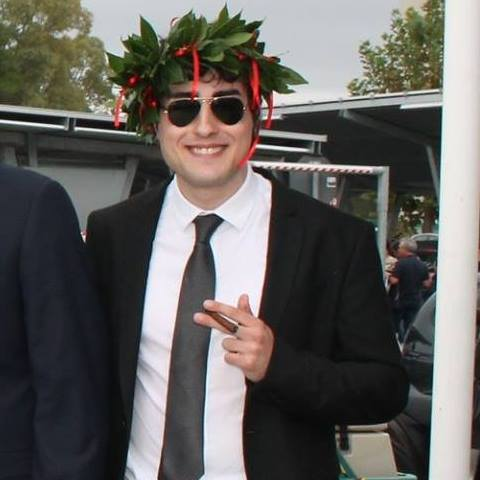
\includegraphics[width=3cm]{figures/marco.jpg}
\vspace{0.3cm}

\raisebox{-0.35ex}{
\includegraphics[width=4ex]{figures/link.png}}%
\hspace{0.05cm} /marcochiarelli

\end{figure}



%BIBLIOGRAFIA - redatta con il relativo ambiente
\begin{thebibliography}{100}
\bibitem{rif1} F. Bullo, J. Cortés, S. Martinez \emph{Distributed Control of Robotic Networks}
\bibitem{rif2} Hassan K. Khalil \emph{Nonlinear System Third Edition}
\bibitem{rif3} Dimitri P. Bertsekas \emph{Nonlinear Programming SECOND EDITION}
\bibitem{rif4} L. Fortuna, M. Frasca \emph{Complementi di Teoria dei Sistemi e di Controlli Automatici}
\end{thebibliography}

\end{document}
